\documentclass[twoside]{book}

% Packages required by doxygen
\usepackage{calc}
\usepackage{doxygen}
\usepackage{graphicx}
\usepackage[utf8]{inputenc}
\usepackage{makeidx}
\usepackage{multicol}
\usepackage{multirow}
\usepackage{textcomp}
\usepackage[table]{xcolor}

% Font selection
\usepackage[T1]{fontenc}
\usepackage{mathptmx}
\usepackage[scaled=.90]{helvet}
\usepackage{courier}
\usepackage{amssymb}
\usepackage{sectsty}
\renewcommand{\familydefault}{\sfdefault}
\allsectionsfont{%
  \fontseries{bc}\selectfont%
  \color{darkgray}%
}
\renewcommand{\DoxyLabelFont}{%
  \fontseries{bc}\selectfont%
  \color{darkgray}%
}

% Page & text layout
\usepackage{geometry}
\geometry{%
  a4paper,%
  top=2.5cm,%
  bottom=2.5cm,%
  left=2.5cm,%
  right=2.5cm%
}
\tolerance=750
\hfuzz=15pt
\hbadness=750
\setlength{\emergencystretch}{15pt}
\setlength{\parindent}{0cm}
\setlength{\parskip}{0.2cm}
\makeatletter
\renewcommand{\paragraph}{%
  \@startsection{paragraph}{4}{0ex}{-1.0ex}{1.0ex}{%
    \normalfont\normalsize\bfseries\SS@parafont%
  }%
}
\renewcommand{\subparagraph}{%
  \@startsection{subparagraph}{5}{0ex}{-1.0ex}{1.0ex}{%
    \normalfont\normalsize\bfseries\SS@subparafont%
  }%
}
\makeatother

% Headers & footers
\usepackage{fancyhdr}
\pagestyle{fancyplain}
\fancyhead[LE]{\fancyplain{}{\bfseries\thepage}}
\fancyhead[CE]{\fancyplain{}{}}
\fancyhead[RE]{\fancyplain{}{\bfseries\leftmark}}
\fancyhead[LO]{\fancyplain{}{\bfseries\rightmark}}
\fancyhead[CO]{\fancyplain{}{}}
\fancyhead[RO]{\fancyplain{}{\bfseries\thepage}}
\fancyfoot[LE]{\fancyplain{}{}}
\fancyfoot[CE]{\fancyplain{}{}}
\fancyfoot[RE]{\fancyplain{}{\bfseries\scriptsize Generated on Tue Sep 15 2015 11\-:05\-:38 for moo-\/java by Doxygen }}
\fancyfoot[LO]{\fancyplain{}{\bfseries\scriptsize Generated on Tue Sep 15 2015 11\-:05\-:38 for moo-\/java by Doxygen }}
\fancyfoot[CO]{\fancyplain{}{}}
\fancyfoot[RO]{\fancyplain{}{}}
\renewcommand{\footrulewidth}{0.4pt}
\renewcommand{\chaptermark}[1]{%
  \markboth{#1}{}%
}
\renewcommand{\sectionmark}[1]{%
  \markright{\thesection\ #1}%
}

% Indices & bibliography
\usepackage{natbib}
\usepackage[titles]{tocloft}
\setcounter{tocdepth}{3}
\setcounter{secnumdepth}{5}
\makeindex

% Hyperlinks (required, but should be loaded last)
\usepackage{ifpdf}
\ifpdf
  \usepackage[pdftex,pagebackref=true]{hyperref}
\else
  \usepackage[ps2pdf,pagebackref=true]{hyperref}
\fi
\hypersetup{%
  colorlinks=true,%
  linkcolor=blue,%
  citecolor=blue,%
  unicode%
}

% Custom commands
\newcommand{\clearemptydoublepage}{%
  \newpage{\pagestyle{empty}\cleardoublepage}%
}


%===== C O N T E N T S =====

\begin{document}

% Titlepage & ToC
\hypersetup{pageanchor=false}
\pagenumbering{roman}
\begin{titlepage}
\vspace*{7cm}
\begin{center}%
{\Large moo-\/java }\\
\vspace*{1cm}
{\large Generated by Doxygen 1.8.6}\\
\vspace*{0.5cm}
{\small Tue Sep 15 2015 11:05:38}\\
\end{center}
\end{titlepage}
\clearemptydoublepage
\tableofcontents
\clearemptydoublepage
\pagenumbering{arabic}
\hypersetup{pageanchor=true}

%--- Begin generated contents ---
\chapter{Hierarchical Index}
\section{Class Hierarchy}
This inheritance list is sorted roughly, but not completely, alphabetically\-:\begin{DoxyCompactList}
\item \contentsline{section}{com.\-msu.\-moo.\-operators.\-Abstract\-Crossover$<$ T $>$}{\pageref{classcom_1_1msu_1_1moo_1_1operators_1_1AbstractCrossover_3_01T_01_4}}{}
\item Abstract\-Experiment\begin{DoxyCompactList}
\item \contentsline{section}{com.\-msu.\-moo.\-experiment.\-N\-Problem\-N\-Algorithm\-Experiment$<$ P extends I\-Problem $>$}{\pageref{classcom_1_1msu_1_1moo_1_1experiment_1_1NProblemNAlgorithmExperiment_3_01P_01extends_01IProblem_01_4}}{}
\item \contentsline{section}{com.\-msu.\-moo.\-experiment.\-One\-Problem\-One\-Algorithm\-Experiment$<$ P extends I\-Problem $>$}{\pageref{classcom_1_1msu_1_1moo_1_1experiment_1_1OneProblemOneAlgorithmExperiment_3_01P_01extends_01IProblem_01_4}}{}
\end{DoxyCompactList}
\item \contentsline{section}{com.\-msu.\-moo.\-experiment.\-Abstract\-Experiment$<$ P extends I\-Problem $>$}{\pageref{classcom_1_1msu_1_1moo_1_1experiment_1_1AbstractExperiment_3_01P_01extends_01IProblem_01_4}}{}
\item \contentsline{section}{com.\-msu.\-moo.\-operators.\-Abstract\-Mutation$<$ T $>$}{\pageref{classcom_1_1msu_1_1moo_1_1operators_1_1AbstractMutation_3_01T_01_4}}{}
\item \contentsline{section}{com.\-msu.\-moo.\-operators.\-Abstract\-Selection}{\pageref{classcom_1_1msu_1_1moo_1_1operators_1_1AbstractSelection}}{}
\begin{DoxyCompactList}
\item \contentsline{section}{com.\-msu.\-moo.\-operators.\-selection.\-Binary\-Tournament\-Selection}{\pageref{classcom_1_1msu_1_1moo_1_1operators_1_1selection_1_1BinaryTournamentSelection}}{}
\end{DoxyCompactList}
\item \contentsline{section}{com.\-msu.\-moo.\-util.\-Bash\-Executor}{\pageref{classcom_1_1msu_1_1moo_1_1util_1_1BashExecutor}}{}
\item \contentsline{section}{com.\-msu.\-moo.\-Configuration}{\pageref{classcom_1_1msu_1_1moo_1_1Configuration}}{}
\item \contentsline{section}{com.\-msu.\-moo.\-operators.\-crossover.\-Crossover\-Util}{\pageref{classcom_1_1msu_1_1moo_1_1operators_1_1crossover_1_1CrossoverUtil}}{}
\item \contentsline{section}{com.\-msu.\-moo.\-fonseca.\-Empirical\-Attainment\-Function}{\pageref{classcom_1_1msu_1_1moo_1_1fonseca_1_1EmpiricalAttainmentFunction}}{}
\item \contentsline{section}{com.\-msu.\-moo.\-experiment.\-Experiment\-Result}{\pageref{classcom_1_1msu_1_1moo_1_1experiment_1_1ExperimentResult}}{}
\item \contentsline{section}{com.\-msu.\-moo.\-fonseca.\-Fonseca\-Util}{\pageref{classcom_1_1msu_1_1moo_1_1fonseca_1_1FonsecaUtil}}{}
\item \contentsline{section}{com.\-msu.\-moo.\-util.\-Front\-Util}{\pageref{classcom_1_1msu_1_1moo_1_1util_1_1FrontUtil}}{}
\item \contentsline{section}{com.\-msu.\-moo.\-fonseca.\-Hypervolume}{\pageref{classcom_1_1msu_1_1moo_1_1fonseca_1_1Hypervolume}}{}
\item \contentsline{section}{com.\-msu.\-moo.\-model.\-interfaces.\-I\-Algorithm$<$ P extends I\-Problem $>$}{\pageref{interfacecom_1_1msu_1_1moo_1_1model_1_1interfaces_1_1IAlgorithm_3_01P_01extends_01IProblem_01_4}}{}
\item \contentsline{section}{com.\-msu.\-moo.\-model.\-interfaces.\-I\-Factory$<$ T extends I\-Variable $>$}{\pageref{interfacecom_1_1msu_1_1moo_1_1model_1_1interfaces_1_1IFactory_3_01T_01extends_01IVariable_01_4}}{}
\item Indicator\begin{DoxyCompactList}
\item \contentsline{section}{com.\-msu.\-moo.\-util.\-indicator.\-Crowding\-Indicator}{\pageref{classcom_1_1msu_1_1moo_1_1util_1_1indicator_1_1CrowdingIndicator}}{}
\item \contentsline{section}{com.\-msu.\-moo.\-util.\-indicator.\-Non\-Dominated\-Rank\-Indicator}{\pageref{classcom_1_1msu_1_1moo_1_1util_1_1indicator_1_1NonDominatedRankIndicator}}{}
\end{DoxyCompactList}
\item \contentsline{section}{com.\-msu.\-moo.\-util.\-indicator.\-Indicator$<$ T $>$}{\pageref{classcom_1_1msu_1_1moo_1_1util_1_1indicator_1_1Indicator_3_01T_01_4}}{}
\item \contentsline{section}{com.\-msu.\-moo.\-visualization.\-I\-Plot}{\pageref{interfacecom_1_1msu_1_1moo_1_1visualization_1_1IPlot}}{}
\begin{DoxyCompactList}
\item \contentsline{section}{com.\-msu.\-moo.\-visualization.\-Abstract2\-D\-Plot}{\pageref{classcom_1_1msu_1_1moo_1_1visualization_1_1Abstract2DPlot}}{}
\begin{DoxyCompactList}
\item \contentsline{section}{com.\-msu.\-moo.\-visualization.\-Box\-Plot}{\pageref{classcom_1_1msu_1_1moo_1_1visualization_1_1BoxPlot}}{}
\item \contentsline{section}{com.\-msu.\-moo.\-visualization.\-Line\-Plot}{\pageref{classcom_1_1msu_1_1moo_1_1visualization_1_1LinePlot}}{}
\item \contentsline{section}{com.\-msu.\-moo.\-visualization.\-Scatter\-Plot}{\pageref{classcom_1_1msu_1_1moo_1_1visualization_1_1ScatterPlot}}{}
\end{DoxyCompactList}
\end{DoxyCompactList}
\item \contentsline{section}{com.\-msu.\-moo.\-model.\-interfaces.\-I\-Problem}{\pageref{interfacecom_1_1msu_1_1moo_1_1model_1_1interfaces_1_1IProblem}}{}
\begin{DoxyCompactList}
\item \contentsline{section}{com.\-msu.\-moo.\-model.\-Abstract\-Problem$<$ V extends I\-Variable $>$}{\pageref{classcom_1_1msu_1_1moo_1_1model_1_1AbstractProblem_3_01V_01extends_01IVariable_01_4}}{}
\end{DoxyCompactList}
\item \contentsline{section}{com.\-msu.\-moo.\-model.\-interfaces.\-I\-Variable}{\pageref{interfacecom_1_1msu_1_1moo_1_1model_1_1interfaces_1_1IVariable}}{}
\begin{DoxyCompactList}
\item \contentsline{section}{com.\-msu.\-moo.\-model.\-Abstract\-Variable$<$ T $>$}{\pageref{classcom_1_1msu_1_1moo_1_1model_1_1AbstractVariable_3_01T_01_4}}{}
\end{DoxyCompactList}
\item List\-Variable\begin{DoxyCompactList}
\item \contentsline{section}{com.\-msu.\-moo.\-model.\-variables.\-Double\-List\-Variable}{\pageref{classcom_1_1msu_1_1moo_1_1model_1_1variables_1_1DoubleListVariable}}{}
\end{DoxyCompactList}
\item \contentsline{section}{com.\-msu.\-moo.\-model.\-solution.\-Non\-Dominated\-Solution\-Set}{\pageref{classcom_1_1msu_1_1moo_1_1model_1_1solution_1_1NonDominatedSolutionSet}}{}
\item \contentsline{section}{com.\-msu.\-moo.\-util.\-sorting.\-Non\-Dominated\-Sorting}{\pageref{interfacecom_1_1msu_1_1moo_1_1util_1_1sorting_1_1NonDominatedSorting}}{}
\begin{DoxyCompactList}
\item \contentsline{section}{com.\-msu.\-moo.\-util.\-sorting.\-Naive\-Non\-Dominated\-Sorting}{\pageref{classcom_1_1msu_1_1moo_1_1util_1_1sorting_1_1NaiveNonDominatedSorting}}{}
\end{DoxyCompactList}
\item N\-Problem\-N\-Algorithm\-Experiment\begin{DoxyCompactList}
\item \contentsline{section}{com.\-msu.\-moo.\-experiment.\-One\-Problem\-N\-Algorithm\-Experiment$<$ P extends I\-Problem $>$}{\pageref{classcom_1_1msu_1_1moo_1_1experiment_1_1OneProblemNAlgorithmExperiment_3_01P_01extends_01IProblem_01_4}}{}
\end{DoxyCompactList}
\item \contentsline{section}{com.\-msu.\-moo.\-algorithms.\-N\-S\-G\-A\-I\-I\-Builder$<$ V extends I\-Variable, P extends I\-Problem $>$}{\pageref{classcom_1_1msu_1_1moo_1_1algorithms_1_1NSGAIIBuilder_3_01V_01extends_01IVariable_00_01P_01extends_01IProblem_01_4}}{}
\item \contentsline{section}{com.\-msu.\-moo.\-util.\-Object\-Factory}{\pageref{classcom_1_1msu_1_1moo_1_1util_1_1ObjectFactory}}{}
\item \contentsline{section}{com.\-msu.\-moo.\-util.\-Pair$<$ F, S $>$}{\pageref{classcom_1_1msu_1_1moo_1_1util_1_1Pair_3_01F_00_01S_01_4}}{}
\item \contentsline{section}{com.\-msu.\-moo.\-util.\-Random}{\pageref{classcom_1_1msu_1_1moo_1_1util_1_1Random}}{}
\item \contentsline{section}{com.\-msu.\-moo.\-util.\-Range$<$ T extends Comparable$<$ T $>$ $>$}{\pageref{classcom_1_1msu_1_1moo_1_1util_1_1Range_3_01T_01extends_01Comparable_3_01T_01_4_01_4}}{}
\item \contentsline{section}{com.\-msu.\-moo.\-model.\-solution.\-Solution}{\pageref{classcom_1_1msu_1_1moo_1_1model_1_1solution_1_1Solution}}{}
\item \contentsline{section}{com.\-msu.\-moo.\-model.\-solution.\-Solution\-Dominator}{\pageref{classcom_1_1msu_1_1moo_1_1model_1_1solution_1_1SolutionDominator}}{}
\item \contentsline{section}{com.\-msu.\-moo.\-util.\-Util}{\pageref{classcom_1_1msu_1_1moo_1_1util_1_1Util}}{}
\item \contentsline{section}{com.\-msu.\-moo.\-model.\-interfaces.\-Variable\-Factory$<$ V extends I\-Variable, P extends I\-Problem $>$}{\pageref{interfacecom_1_1msu_1_1moo_1_1model_1_1interfaces_1_1VariableFactory_3_01V_01extends_01IVariablebc6c2f25a98dd397b069d7e08412a00f}}{}
\item Abstract\-Algorithm\begin{DoxyCompactList}
\item \contentsline{section}{com.\-msu.\-moo.\-algorithms.\-Exhaustive\-Solver$<$ V extends I\-Variable, P extends I\-Problem $>$}{\pageref{classcom_1_1msu_1_1moo_1_1algorithms_1_1ExhaustiveSolver_3_01V_01extends_01IVariable_00_01P_01extends_01IProblem_01_4}}{}
\item \contentsline{section}{com.\-msu.\-moo.\-algorithms.\-N\-S\-G\-A\-I\-I$<$ V extends I\-Variable, P extends I\-Problem $>$}{\pageref{classcom_1_1msu_1_1moo_1_1algorithms_1_1NSGAII_3_01V_01extends_01IVariable_00_01P_01extends_01IProblem_01_4}}{}
\item \contentsline{section}{com.\-msu.\-moo.\-algorithms.\-Random\-Search$<$ V extends I\-Variable, P extends I\-Problem $>$}{\pageref{classcom_1_1msu_1_1moo_1_1algorithms_1_1RandomSearch_3_01V_01extends_01IVariable_00_01P_01extends_01IProblem_01_4}}{}
\end{DoxyCompactList}
\item Abstract\-Crossover\begin{DoxyCompactList}
\item \contentsline{section}{com.\-msu.\-moo.\-operators.\-Abstract\-List\-Crossover$<$ T $>$}{\pageref{classcom_1_1msu_1_1moo_1_1operators_1_1AbstractListCrossover_3_01T_01_4}}{}
\end{DoxyCompactList}
\item Abstract\-List\-Crossover\begin{DoxyCompactList}
\item \contentsline{section}{com.\-msu.\-moo.\-operators.\-crossover.\-Half\-Uniform\-Crossover$<$ T $>$}{\pageref{classcom_1_1msu_1_1moo_1_1operators_1_1crossover_1_1HalfUniformCrossover_3_01T_01_4}}{}
\item \contentsline{section}{com.\-msu.\-moo.\-operators.\-crossover.\-N\-Point\-Crossover$<$ T $>$}{\pageref{classcom_1_1msu_1_1moo_1_1operators_1_1crossover_1_1NPointCrossover_3_01T_01_4}}{}
\item \contentsline{section}{com.\-msu.\-moo.\-operators.\-crossover.\-permutation.\-Cycle\-Crossover$<$ T $>$}{\pageref{classcom_1_1msu_1_1moo_1_1operators_1_1crossover_1_1permutation_1_1CycleCrossover_3_01T_01_4}}{}
\item \contentsline{section}{com.\-msu.\-moo.\-operators.\-crossover.\-permutation.\-Edge\-Recombination\-Crossover$<$ T $>$}{\pageref{classcom_1_1msu_1_1moo_1_1operators_1_1crossover_1_1permutation_1_1EdgeRecombinationCrossover_3_01T_01_4}}{}
\item \contentsline{section}{com.\-msu.\-moo.\-operators.\-crossover.\-permutation.\-Ordered\-Crossover$<$ T $>$}{\pageref{classcom_1_1msu_1_1moo_1_1operators_1_1crossover_1_1permutation_1_1OrderedCrossover_3_01T_01_4}}{}
\item \contentsline{section}{com.\-msu.\-moo.\-operators.\-crossover.\-permutation.\-P\-M\-X\-Crossover$<$ T $>$}{\pageref{classcom_1_1msu_1_1moo_1_1operators_1_1crossover_1_1permutation_1_1PMXCrossover_3_01T_01_4}}{}
\item \contentsline{section}{com.\-msu.\-moo.\-operators.\-crossover.\-Simulated\-Binary\-Crossover}{\pageref{classcom_1_1msu_1_1moo_1_1operators_1_1crossover_1_1SimulatedBinaryCrossover}}{}
\item \contentsline{section}{com.\-msu.\-moo.\-operators.\-crossover.\-Single\-Point\-Crossover$<$ T $>$}{\pageref{classcom_1_1msu_1_1moo_1_1operators_1_1crossover_1_1SinglePointCrossover_3_01T_01_4}}{}
\item \contentsline{section}{com.\-msu.\-moo.\-operators.\-crossover.\-Uniform\-Crossover$<$ T $>$}{\pageref{classcom_1_1msu_1_1moo_1_1operators_1_1crossover_1_1UniformCrossover_3_01T_01_4}}{}
\end{DoxyCompactList}
\item Abstract\-Mutation\begin{DoxyCompactList}
\item \contentsline{section}{com.\-msu.\-moo.\-operators.\-mutation.\-Bit\-Flip\-Mutation}{\pageref{classcom_1_1msu_1_1moo_1_1operators_1_1mutation_1_1BitFlipMutation}}{}
\item \contentsline{section}{com.\-msu.\-moo.\-operators.\-mutation.\-Polynomial\-Mutation}{\pageref{classcom_1_1msu_1_1moo_1_1operators_1_1mutation_1_1PolynomialMutation}}{}
\item \contentsline{section}{com.\-msu.\-moo.\-operators.\-mutation.\-Real\-Mutation}{\pageref{classcom_1_1msu_1_1moo_1_1operators_1_1mutation_1_1RealMutation}}{}
\item \contentsline{section}{com.\-msu.\-moo.\-operators.\-mutation.\-Restricted\-Polynomial\-Mutation}{\pageref{classcom_1_1msu_1_1moo_1_1operators_1_1mutation_1_1RestrictedPolynomialMutation}}{}
\item \contentsline{section}{com.\-msu.\-moo.\-operators.\-mutation.\-Swap\-Mutation$<$ T $>$}{\pageref{classcom_1_1msu_1_1moo_1_1operators_1_1mutation_1_1SwapMutation_3_01T_01_4}}{}
\end{DoxyCompactList}
\item Abstract\-Problem\begin{DoxyCompactList}
\item \contentsline{section}{com.\-msu.\-moo.\-problems.\-Kursawe}{\pageref{classcom_1_1msu_1_1moo_1_1problems_1_1Kursawe}}{}
\item \contentsline{section}{com.\-msu.\-moo.\-problems.\-Z\-D\-T1}{\pageref{classcom_1_1msu_1_1moo_1_1problems_1_1ZDT1}}{}
\end{DoxyCompactList}
\item Abstract\-Variable\begin{DoxyCompactList}
\item \contentsline{section}{com.\-msu.\-moo.\-model.\-variables.\-List\-Variable$<$ T $>$}{\pageref{classcom_1_1msu_1_1moo_1_1model_1_1variables_1_1ListVariable_3_01T_01_4}}{}
\end{DoxyCompactList}
\item Array\-List\begin{DoxyCompactList}
\item \contentsline{section}{com.\-msu.\-moo.\-model.\-solution.\-Solution\-Set}{\pageref{classcom_1_1msu_1_1moo_1_1model_1_1solution_1_1SolutionSet}}{}
\end{DoxyCompactList}
\item Comparator\begin{DoxyCompactList}
\item \contentsline{section}{com.\-msu.\-moo.\-util.\-comparator.\-Rank\-And\-Crowding\-Comparator}{\pageref{classcom_1_1msu_1_1moo_1_1util_1_1comparator_1_1RankAndCrowdingComparator}}{}
\end{DoxyCompactList}
\item I\-Algorithm\begin{DoxyCompactList}
\item \contentsline{section}{com.\-msu.\-moo.\-model.\-Abstract\-Algorithm$<$ V extends I\-Variable, P extends I\-Problem $>$}{\pageref{classcom_1_1msu_1_1moo_1_1model_1_1AbstractAlgorithm_3_01V_01extends_01IVariable_00_01P_01extends_01IProblem_01_4}}{}
\end{DoxyCompactList}
\item One\-Problem\-N\-Algorithm\-Experiment\begin{DoxyCompactList}
\item \contentsline{section}{com.\-msu.\-moo.\-experiment.\-impl.\-Kursawe\-Experiment}{\pageref{classcom_1_1msu_1_1moo_1_1experiment_1_1impl_1_1KursaweExperiment}}{}
\end{DoxyCompactList}
\item One\-Problem\-One\-Algorithm\-Experiment\begin{DoxyCompactList}
\item \contentsline{section}{com.\-msu.\-moo.\-experiment.\-impl.\-Z\-D\-T1\-Experiment}{\pageref{classcom_1_1msu_1_1moo_1_1experiment_1_1impl_1_1ZDT1Experiment}}{}
\end{DoxyCompactList}
\item Variable\-Factory\begin{DoxyCompactList}
\item \contentsline{section}{com.\-msu.\-moo.\-model.\-variables.\-Double\-List\-Variable\-Factory$<$ P extends I\-Problem $>$}{\pageref{classcom_1_1msu_1_1moo_1_1model_1_1variables_1_1DoubleListVariableFactory_3_01P_01extends_01IProblem_01_4}}{}
\end{DoxyCompactList}
\end{DoxyCompactList}

\chapter{Class Index}
\section{Class List}
Here are the classes, structs, unions and interfaces with brief descriptions\-:\begin{DoxyCompactList}
\item\contentsline{section}{\hyperlink{classcom_1_1msu_1_1moo_1_1visualization_1_1Abstract2DPlot}{com.\-msu.\-moo.\-visualization.\-Abstract2\-D\-Plot} }{\pageref{classcom_1_1msu_1_1moo_1_1visualization_1_1Abstract2DPlot}}{}
\item\contentsline{section}{\hyperlink{classcom_1_1msu_1_1moo_1_1model_1_1AbstractAlgorithm_3_01V_01extends_01IVariable_00_01P_01extends_01IProblem_01_4}{com.\-msu.\-moo.\-model.\-Abstract\-Algorithm$<$ V extends I\-Variable, P extends I\-Problem $>$} }{\pageref{classcom_1_1msu_1_1moo_1_1model_1_1AbstractAlgorithm_3_01V_01extends_01IVariable_00_01P_01extends_01IProblem_01_4}}{}
\item\contentsline{section}{\hyperlink{classcom_1_1msu_1_1moo_1_1operators_1_1AbstractCrossover_3_01T_01_4}{com.\-msu.\-moo.\-operators.\-Abstract\-Crossover$<$ T $>$} }{\pageref{classcom_1_1msu_1_1moo_1_1operators_1_1AbstractCrossover_3_01T_01_4}}{}
\item\contentsline{section}{\hyperlink{classcom_1_1msu_1_1moo_1_1experiment_1_1AbstractExperiment_3_01P_01extends_01IProblem_01_4}{com.\-msu.\-moo.\-experiment.\-Abstract\-Experiment$<$ P extends I\-Problem $>$} }{\pageref{classcom_1_1msu_1_1moo_1_1experiment_1_1AbstractExperiment_3_01P_01extends_01IProblem_01_4}}{}
\item\contentsline{section}{\hyperlink{classcom_1_1msu_1_1moo_1_1operators_1_1AbstractListCrossover_3_01T_01_4}{com.\-msu.\-moo.\-operators.\-Abstract\-List\-Crossover$<$ T $>$} }{\pageref{classcom_1_1msu_1_1moo_1_1operators_1_1AbstractListCrossover_3_01T_01_4}}{}
\item\contentsline{section}{\hyperlink{classcom_1_1msu_1_1moo_1_1operators_1_1AbstractMutation_3_01T_01_4}{com.\-msu.\-moo.\-operators.\-Abstract\-Mutation$<$ T $>$} }{\pageref{classcom_1_1msu_1_1moo_1_1operators_1_1AbstractMutation_3_01T_01_4}}{}
\item\contentsline{section}{\hyperlink{classcom_1_1msu_1_1moo_1_1model_1_1AbstractProblem_3_01V_01extends_01IVariable_01_4}{com.\-msu.\-moo.\-model.\-Abstract\-Problem$<$ V extends I\-Variable $>$} }{\pageref{classcom_1_1msu_1_1moo_1_1model_1_1AbstractProblem_3_01V_01extends_01IVariable_01_4}}{}
\item\contentsline{section}{\hyperlink{classcom_1_1msu_1_1moo_1_1operators_1_1AbstractSelection}{com.\-msu.\-moo.\-operators.\-Abstract\-Selection} }{\pageref{classcom_1_1msu_1_1moo_1_1operators_1_1AbstractSelection}}{}
\item\contentsline{section}{\hyperlink{classcom_1_1msu_1_1moo_1_1model_1_1AbstractVariable_3_01T_01_4}{com.\-msu.\-moo.\-model.\-Abstract\-Variable$<$ T $>$} }{\pageref{classcom_1_1msu_1_1moo_1_1model_1_1AbstractVariable_3_01T_01_4}}{}
\item\contentsline{section}{\hyperlink{classcom_1_1msu_1_1moo_1_1util_1_1BashExecutor}{com.\-msu.\-moo.\-util.\-Bash\-Executor} }{\pageref{classcom_1_1msu_1_1moo_1_1util_1_1BashExecutor}}{}
\item\contentsline{section}{\hyperlink{classcom_1_1msu_1_1moo_1_1operators_1_1selection_1_1BinaryTournamentSelection}{com.\-msu.\-moo.\-operators.\-selection.\-Binary\-Tournament\-Selection} }{\pageref{classcom_1_1msu_1_1moo_1_1operators_1_1selection_1_1BinaryTournamentSelection}}{}
\item\contentsline{section}{\hyperlink{classcom_1_1msu_1_1moo_1_1operators_1_1mutation_1_1BitFlipMutation}{com.\-msu.\-moo.\-operators.\-mutation.\-Bit\-Flip\-Mutation} }{\pageref{classcom_1_1msu_1_1moo_1_1operators_1_1mutation_1_1BitFlipMutation}}{}
\item\contentsline{section}{\hyperlink{classcom_1_1msu_1_1moo_1_1visualization_1_1BoxPlot}{com.\-msu.\-moo.\-visualization.\-Box\-Plot} }{\pageref{classcom_1_1msu_1_1moo_1_1visualization_1_1BoxPlot}}{}
\item\contentsline{section}{\hyperlink{classcom_1_1msu_1_1moo_1_1Configuration}{com.\-msu.\-moo.\-Configuration} }{\pageref{classcom_1_1msu_1_1moo_1_1Configuration}}{}
\item\contentsline{section}{\hyperlink{classcom_1_1msu_1_1moo_1_1operators_1_1crossover_1_1CrossoverUtil}{com.\-msu.\-moo.\-operators.\-crossover.\-Crossover\-Util} }{\pageref{classcom_1_1msu_1_1moo_1_1operators_1_1crossover_1_1CrossoverUtil}}{}
\item\contentsline{section}{\hyperlink{classcom_1_1msu_1_1moo_1_1util_1_1indicator_1_1CrowdingIndicator}{com.\-msu.\-moo.\-util.\-indicator.\-Crowding\-Indicator} }{\pageref{classcom_1_1msu_1_1moo_1_1util_1_1indicator_1_1CrowdingIndicator}}{}
\item\contentsline{section}{\hyperlink{classcom_1_1msu_1_1moo_1_1operators_1_1crossover_1_1permutation_1_1CycleCrossover_3_01T_01_4}{com.\-msu.\-moo.\-operators.\-crossover.\-permutation.\-Cycle\-Crossover$<$ T $>$} }{\pageref{classcom_1_1msu_1_1moo_1_1operators_1_1crossover_1_1permutation_1_1CycleCrossover_3_01T_01_4}}{}
\item\contentsline{section}{\hyperlink{classcom_1_1msu_1_1moo_1_1model_1_1variables_1_1DoubleListVariable}{com.\-msu.\-moo.\-model.\-variables.\-Double\-List\-Variable} }{\pageref{classcom_1_1msu_1_1moo_1_1model_1_1variables_1_1DoubleListVariable}}{}
\item\contentsline{section}{\hyperlink{classcom_1_1msu_1_1moo_1_1model_1_1variables_1_1DoubleListVariableFactory_3_01P_01extends_01IProblem_01_4}{com.\-msu.\-moo.\-model.\-variables.\-Double\-List\-Variable\-Factory$<$ P extends I\-Problem $>$} }{\pageref{classcom_1_1msu_1_1moo_1_1model_1_1variables_1_1DoubleListVariableFactory_3_01P_01extends_01IProblem_01_4}}{}
\item\contentsline{section}{\hyperlink{classcom_1_1msu_1_1moo_1_1operators_1_1crossover_1_1permutation_1_1EdgeRecombinationCrossover_3_01T_01_4}{com.\-msu.\-moo.\-operators.\-crossover.\-permutation.\-Edge\-Recombination\-Crossover$<$ T $>$} }{\pageref{classcom_1_1msu_1_1moo_1_1operators_1_1crossover_1_1permutation_1_1EdgeRecombinationCrossover_3_01T_01_4}}{}
\item\contentsline{section}{\hyperlink{classcom_1_1msu_1_1moo_1_1fonseca_1_1EmpiricalAttainmentFunction}{com.\-msu.\-moo.\-fonseca.\-Empirical\-Attainment\-Function} }{\pageref{classcom_1_1msu_1_1moo_1_1fonseca_1_1EmpiricalAttainmentFunction}}{}
\item\contentsline{section}{\hyperlink{classcom_1_1msu_1_1moo_1_1algorithms_1_1ExhaustiveSolver_3_01V_01extends_01IVariable_00_01P_01extends_01IProblem_01_4}{com.\-msu.\-moo.\-algorithms.\-Exhaustive\-Solver$<$ V extends I\-Variable, P extends I\-Problem $>$} }{\pageref{classcom_1_1msu_1_1moo_1_1algorithms_1_1ExhaustiveSolver_3_01V_01extends_01IVariable_00_01P_01extends_01IProblem_01_4}}{}
\item\contentsline{section}{\hyperlink{classcom_1_1msu_1_1moo_1_1experiment_1_1ExperimentResult}{com.\-msu.\-moo.\-experiment.\-Experiment\-Result} }{\pageref{classcom_1_1msu_1_1moo_1_1experiment_1_1ExperimentResult}}{}
\item\contentsline{section}{\hyperlink{classcom_1_1msu_1_1moo_1_1fonseca_1_1FonsecaUtil}{com.\-msu.\-moo.\-fonseca.\-Fonseca\-Util} }{\pageref{classcom_1_1msu_1_1moo_1_1fonseca_1_1FonsecaUtil}}{}
\item\contentsline{section}{\hyperlink{classcom_1_1msu_1_1moo_1_1util_1_1FrontUtil}{com.\-msu.\-moo.\-util.\-Front\-Util} }{\pageref{classcom_1_1msu_1_1moo_1_1util_1_1FrontUtil}}{}
\item\contentsline{section}{\hyperlink{classcom_1_1msu_1_1moo_1_1operators_1_1crossover_1_1HalfUniformCrossover_3_01T_01_4}{com.\-msu.\-moo.\-operators.\-crossover.\-Half\-Uniform\-Crossover$<$ T $>$} }{\pageref{classcom_1_1msu_1_1moo_1_1operators_1_1crossover_1_1HalfUniformCrossover_3_01T_01_4}}{}
\item\contentsline{section}{\hyperlink{classcom_1_1msu_1_1moo_1_1fonseca_1_1Hypervolume}{com.\-msu.\-moo.\-fonseca.\-Hypervolume} }{\pageref{classcom_1_1msu_1_1moo_1_1fonseca_1_1Hypervolume}}{}
\item\contentsline{section}{\hyperlink{interfacecom_1_1msu_1_1moo_1_1model_1_1interfaces_1_1IAlgorithm_3_01P_01extends_01IProblem_01_4}{com.\-msu.\-moo.\-model.\-interfaces.\-I\-Algorithm$<$ P extends I\-Problem $>$} }{\pageref{interfacecom_1_1msu_1_1moo_1_1model_1_1interfaces_1_1IAlgorithm_3_01P_01extends_01IProblem_01_4}}{}
\item\contentsline{section}{\hyperlink{interfacecom_1_1msu_1_1moo_1_1model_1_1interfaces_1_1IFactory_3_01T_01extends_01IVariable_01_4}{com.\-msu.\-moo.\-model.\-interfaces.\-I\-Factory$<$ T extends I\-Variable $>$} }{\pageref{interfacecom_1_1msu_1_1moo_1_1model_1_1interfaces_1_1IFactory_3_01T_01extends_01IVariable_01_4}}{}
\item\contentsline{section}{\hyperlink{classcom_1_1msu_1_1moo_1_1util_1_1indicator_1_1Indicator_3_01T_01_4}{com.\-msu.\-moo.\-util.\-indicator.\-Indicator$<$ T $>$} }{\pageref{classcom_1_1msu_1_1moo_1_1util_1_1indicator_1_1Indicator_3_01T_01_4}}{}
\item\contentsline{section}{\hyperlink{interfacecom_1_1msu_1_1moo_1_1visualization_1_1IPlot}{com.\-msu.\-moo.\-visualization.\-I\-Plot} }{\pageref{interfacecom_1_1msu_1_1moo_1_1visualization_1_1IPlot}}{}
\item\contentsline{section}{\hyperlink{interfacecom_1_1msu_1_1moo_1_1model_1_1interfaces_1_1IProblem}{com.\-msu.\-moo.\-model.\-interfaces.\-I\-Problem} }{\pageref{interfacecom_1_1msu_1_1moo_1_1model_1_1interfaces_1_1IProblem}}{}
\item\contentsline{section}{\hyperlink{interfacecom_1_1msu_1_1moo_1_1model_1_1interfaces_1_1IVariable}{com.\-msu.\-moo.\-model.\-interfaces.\-I\-Variable} }{\pageref{interfacecom_1_1msu_1_1moo_1_1model_1_1interfaces_1_1IVariable}}{}
\item\contentsline{section}{\hyperlink{classcom_1_1msu_1_1moo_1_1problems_1_1Kursawe}{com.\-msu.\-moo.\-problems.\-Kursawe} }{\pageref{classcom_1_1msu_1_1moo_1_1problems_1_1Kursawe}}{}
\item\contentsline{section}{\hyperlink{classcom_1_1msu_1_1moo_1_1experiment_1_1impl_1_1KursaweExperiment}{com.\-msu.\-moo.\-experiment.\-impl.\-Kursawe\-Experiment} }{\pageref{classcom_1_1msu_1_1moo_1_1experiment_1_1impl_1_1KursaweExperiment}}{}
\item\contentsline{section}{\hyperlink{classcom_1_1msu_1_1moo_1_1visualization_1_1LinePlot}{com.\-msu.\-moo.\-visualization.\-Line\-Plot} }{\pageref{classcom_1_1msu_1_1moo_1_1visualization_1_1LinePlot}}{}
\item\contentsline{section}{\hyperlink{classcom_1_1msu_1_1moo_1_1model_1_1variables_1_1ListVariable_3_01T_01_4}{com.\-msu.\-moo.\-model.\-variables.\-List\-Variable$<$ T $>$} }{\pageref{classcom_1_1msu_1_1moo_1_1model_1_1variables_1_1ListVariable_3_01T_01_4}}{}
\item\contentsline{section}{\hyperlink{classcom_1_1msu_1_1moo_1_1util_1_1sorting_1_1NaiveNonDominatedSorting}{com.\-msu.\-moo.\-util.\-sorting.\-Naive\-Non\-Dominated\-Sorting} }{\pageref{classcom_1_1msu_1_1moo_1_1util_1_1sorting_1_1NaiveNonDominatedSorting}}{}
\item\contentsline{section}{\hyperlink{classcom_1_1msu_1_1moo_1_1util_1_1indicator_1_1NonDominatedRankIndicator}{com.\-msu.\-moo.\-util.\-indicator.\-Non\-Dominated\-Rank\-Indicator} }{\pageref{classcom_1_1msu_1_1moo_1_1util_1_1indicator_1_1NonDominatedRankIndicator}}{}
\item\contentsline{section}{\hyperlink{classcom_1_1msu_1_1moo_1_1model_1_1solution_1_1NonDominatedSolutionSet}{com.\-msu.\-moo.\-model.\-solution.\-Non\-Dominated\-Solution\-Set} }{\pageref{classcom_1_1msu_1_1moo_1_1model_1_1solution_1_1NonDominatedSolutionSet}}{}
\item\contentsline{section}{\hyperlink{interfacecom_1_1msu_1_1moo_1_1util_1_1sorting_1_1NonDominatedSorting}{com.\-msu.\-moo.\-util.\-sorting.\-Non\-Dominated\-Sorting} }{\pageref{interfacecom_1_1msu_1_1moo_1_1util_1_1sorting_1_1NonDominatedSorting}}{}
\item\contentsline{section}{\hyperlink{classcom_1_1msu_1_1moo_1_1operators_1_1crossover_1_1NPointCrossover_3_01T_01_4}{com.\-msu.\-moo.\-operators.\-crossover.\-N\-Point\-Crossover$<$ T $>$} }{\pageref{classcom_1_1msu_1_1moo_1_1operators_1_1crossover_1_1NPointCrossover_3_01T_01_4}}{}
\item\contentsline{section}{\hyperlink{classcom_1_1msu_1_1moo_1_1experiment_1_1NProblemNAlgorithmExperiment_3_01P_01extends_01IProblem_01_4}{com.\-msu.\-moo.\-experiment.\-N\-Problem\-N\-Algorithm\-Experiment$<$ P extends I\-Problem $>$} }{\pageref{classcom_1_1msu_1_1moo_1_1experiment_1_1NProblemNAlgorithmExperiment_3_01P_01extends_01IProblem_01_4}}{}
\item\contentsline{section}{\hyperlink{classcom_1_1msu_1_1moo_1_1algorithms_1_1NSGAII_3_01V_01extends_01IVariable_00_01P_01extends_01IProblem_01_4}{com.\-msu.\-moo.\-algorithms.\-N\-S\-G\-A\-I\-I$<$ V extends I\-Variable, P extends I\-Problem $>$} }{\pageref{classcom_1_1msu_1_1moo_1_1algorithms_1_1NSGAII_3_01V_01extends_01IVariable_00_01P_01extends_01IProblem_01_4}}{}
\item\contentsline{section}{\hyperlink{classcom_1_1msu_1_1moo_1_1algorithms_1_1NSGAIIBuilder_3_01V_01extends_01IVariable_00_01P_01extends_01IProblem_01_4}{com.\-msu.\-moo.\-algorithms.\-N\-S\-G\-A\-I\-I\-Builder$<$ V extends I\-Variable, P extends I\-Problem $>$} }{\pageref{classcom_1_1msu_1_1moo_1_1algorithms_1_1NSGAIIBuilder_3_01V_01extends_01IVariable_00_01P_01extends_01IProblem_01_4}}{}
\item\contentsline{section}{\hyperlink{classcom_1_1msu_1_1moo_1_1util_1_1ObjectFactory}{com.\-msu.\-moo.\-util.\-Object\-Factory} }{\pageref{classcom_1_1msu_1_1moo_1_1util_1_1ObjectFactory}}{}
\item\contentsline{section}{\hyperlink{classcom_1_1msu_1_1moo_1_1experiment_1_1OneProblemNAlgorithmExperiment_3_01P_01extends_01IProblem_01_4}{com.\-msu.\-moo.\-experiment.\-One\-Problem\-N\-Algorithm\-Experiment$<$ P extends I\-Problem $>$} }{\pageref{classcom_1_1msu_1_1moo_1_1experiment_1_1OneProblemNAlgorithmExperiment_3_01P_01extends_01IProblem_01_4}}{}
\item\contentsline{section}{\hyperlink{classcom_1_1msu_1_1moo_1_1experiment_1_1OneProblemOneAlgorithmExperiment_3_01P_01extends_01IProblem_01_4}{com.\-msu.\-moo.\-experiment.\-One\-Problem\-One\-Algorithm\-Experiment$<$ P extends I\-Problem $>$} }{\pageref{classcom_1_1msu_1_1moo_1_1experiment_1_1OneProblemOneAlgorithmExperiment_3_01P_01extends_01IProblem_01_4}}{}
\item\contentsline{section}{\hyperlink{classcom_1_1msu_1_1moo_1_1operators_1_1crossover_1_1permutation_1_1OrderedCrossover_3_01T_01_4}{com.\-msu.\-moo.\-operators.\-crossover.\-permutation.\-Ordered\-Crossover$<$ T $>$} }{\pageref{classcom_1_1msu_1_1moo_1_1operators_1_1crossover_1_1permutation_1_1OrderedCrossover_3_01T_01_4}}{}
\item\contentsline{section}{\hyperlink{classcom_1_1msu_1_1moo_1_1util_1_1Pair_3_01F_00_01S_01_4}{com.\-msu.\-moo.\-util.\-Pair$<$ F, S $>$} }{\pageref{classcom_1_1msu_1_1moo_1_1util_1_1Pair_3_01F_00_01S_01_4}}{}
\item\contentsline{section}{\hyperlink{classcom_1_1msu_1_1moo_1_1operators_1_1crossover_1_1permutation_1_1PMXCrossover_3_01T_01_4}{com.\-msu.\-moo.\-operators.\-crossover.\-permutation.\-P\-M\-X\-Crossover$<$ T $>$} }{\pageref{classcom_1_1msu_1_1moo_1_1operators_1_1crossover_1_1permutation_1_1PMXCrossover_3_01T_01_4}}{}
\item\contentsline{section}{\hyperlink{classcom_1_1msu_1_1moo_1_1operators_1_1mutation_1_1PolynomialMutation}{com.\-msu.\-moo.\-operators.\-mutation.\-Polynomial\-Mutation} }{\pageref{classcom_1_1msu_1_1moo_1_1operators_1_1mutation_1_1PolynomialMutation}}{}
\item\contentsline{section}{\hyperlink{classcom_1_1msu_1_1moo_1_1util_1_1Random}{com.\-msu.\-moo.\-util.\-Random} }{\pageref{classcom_1_1msu_1_1moo_1_1util_1_1Random}}{}
\item\contentsline{section}{\hyperlink{classcom_1_1msu_1_1moo_1_1algorithms_1_1RandomSearch_3_01V_01extends_01IVariable_00_01P_01extends_01IProblem_01_4}{com.\-msu.\-moo.\-algorithms.\-Random\-Search$<$ V extends I\-Variable, P extends I\-Problem $>$} }{\pageref{classcom_1_1msu_1_1moo_1_1algorithms_1_1RandomSearch_3_01V_01extends_01IVariable_00_01P_01extends_01IProblem_01_4}}{}
\item\contentsline{section}{\hyperlink{classcom_1_1msu_1_1moo_1_1util_1_1Range_3_01T_01extends_01Comparable_3_01T_01_4_01_4}{com.\-msu.\-moo.\-util.\-Range$<$ T extends Comparable$<$ T $>$ $>$} }{\pageref{classcom_1_1msu_1_1moo_1_1util_1_1Range_3_01T_01extends_01Comparable_3_01T_01_4_01_4}}{}
\item\contentsline{section}{\hyperlink{classcom_1_1msu_1_1moo_1_1util_1_1comparator_1_1RankAndCrowdingComparator}{com.\-msu.\-moo.\-util.\-comparator.\-Rank\-And\-Crowding\-Comparator} }{\pageref{classcom_1_1msu_1_1moo_1_1util_1_1comparator_1_1RankAndCrowdingComparator}}{}
\item\contentsline{section}{\hyperlink{classcom_1_1msu_1_1moo_1_1operators_1_1mutation_1_1RealMutation}{com.\-msu.\-moo.\-operators.\-mutation.\-Real\-Mutation} }{\pageref{classcom_1_1msu_1_1moo_1_1operators_1_1mutation_1_1RealMutation}}{}
\item\contentsline{section}{\hyperlink{classcom_1_1msu_1_1moo_1_1operators_1_1mutation_1_1RestrictedPolynomialMutation}{com.\-msu.\-moo.\-operators.\-mutation.\-Restricted\-Polynomial\-Mutation} }{\pageref{classcom_1_1msu_1_1moo_1_1operators_1_1mutation_1_1RestrictedPolynomialMutation}}{}
\item\contentsline{section}{\hyperlink{classcom_1_1msu_1_1moo_1_1visualization_1_1ScatterPlot}{com.\-msu.\-moo.\-visualization.\-Scatter\-Plot} }{\pageref{classcom_1_1msu_1_1moo_1_1visualization_1_1ScatterPlot}}{}
\item\contentsline{section}{\hyperlink{classcom_1_1msu_1_1moo_1_1operators_1_1crossover_1_1SimulatedBinaryCrossover}{com.\-msu.\-moo.\-operators.\-crossover.\-Simulated\-Binary\-Crossover} }{\pageref{classcom_1_1msu_1_1moo_1_1operators_1_1crossover_1_1SimulatedBinaryCrossover}}{}
\item\contentsline{section}{\hyperlink{classcom_1_1msu_1_1moo_1_1operators_1_1crossover_1_1SinglePointCrossover_3_01T_01_4}{com.\-msu.\-moo.\-operators.\-crossover.\-Single\-Point\-Crossover$<$ T $>$} }{\pageref{classcom_1_1msu_1_1moo_1_1operators_1_1crossover_1_1SinglePointCrossover_3_01T_01_4}}{}
\item\contentsline{section}{\hyperlink{classcom_1_1msu_1_1moo_1_1model_1_1solution_1_1Solution}{com.\-msu.\-moo.\-model.\-solution.\-Solution} }{\pageref{classcom_1_1msu_1_1moo_1_1model_1_1solution_1_1Solution}}{}
\item\contentsline{section}{\hyperlink{classcom_1_1msu_1_1moo_1_1model_1_1solution_1_1SolutionDominator}{com.\-msu.\-moo.\-model.\-solution.\-Solution\-Dominator} }{\pageref{classcom_1_1msu_1_1moo_1_1model_1_1solution_1_1SolutionDominator}}{}
\item\contentsline{section}{\hyperlink{classcom_1_1msu_1_1moo_1_1model_1_1solution_1_1SolutionSet}{com.\-msu.\-moo.\-model.\-solution.\-Solution\-Set} }{\pageref{classcom_1_1msu_1_1moo_1_1model_1_1solution_1_1SolutionSet}}{}
\item\contentsline{section}{\hyperlink{classcom_1_1msu_1_1moo_1_1operators_1_1mutation_1_1SwapMutation_3_01T_01_4}{com.\-msu.\-moo.\-operators.\-mutation.\-Swap\-Mutation$<$ T $>$} }{\pageref{classcom_1_1msu_1_1moo_1_1operators_1_1mutation_1_1SwapMutation_3_01T_01_4}}{}
\item\contentsline{section}{\hyperlink{classcom_1_1msu_1_1moo_1_1operators_1_1crossover_1_1UniformCrossover_3_01T_01_4}{com.\-msu.\-moo.\-operators.\-crossover.\-Uniform\-Crossover$<$ T $>$} }{\pageref{classcom_1_1msu_1_1moo_1_1operators_1_1crossover_1_1UniformCrossover_3_01T_01_4}}{}
\item\contentsline{section}{\hyperlink{classcom_1_1msu_1_1moo_1_1util_1_1Util}{com.\-msu.\-moo.\-util.\-Util} }{\pageref{classcom_1_1msu_1_1moo_1_1util_1_1Util}}{}
\item\contentsline{section}{\hyperlink{interfacecom_1_1msu_1_1moo_1_1model_1_1interfaces_1_1VariableFactory_3_01V_01extends_01IVariablebc6c2f25a98dd397b069d7e08412a00f}{com.\-msu.\-moo.\-model.\-interfaces.\-Variable\-Factory$<$ V extends I\-Variable, P extends I\-Problem $>$} }{\pageref{interfacecom_1_1msu_1_1moo_1_1model_1_1interfaces_1_1VariableFactory_3_01V_01extends_01IVariablebc6c2f25a98dd397b069d7e08412a00f}}{}
\item\contentsline{section}{\hyperlink{classcom_1_1msu_1_1moo_1_1problems_1_1ZDT1}{com.\-msu.\-moo.\-problems.\-Z\-D\-T1} }{\pageref{classcom_1_1msu_1_1moo_1_1problems_1_1ZDT1}}{}
\item\contentsline{section}{\hyperlink{classcom_1_1msu_1_1moo_1_1experiment_1_1impl_1_1ZDT1Experiment}{com.\-msu.\-moo.\-experiment.\-impl.\-Z\-D\-T1\-Experiment} }{\pageref{classcom_1_1msu_1_1moo_1_1experiment_1_1impl_1_1ZDT1Experiment}}{}
\end{DoxyCompactList}

\chapter{Class Documentation}
\hypertarget{classcom_1_1msu_1_1moo_1_1visualization_1_1Abstract2DPlot}{\section{com.\-msu.\-moo.\-visualization.\-Abstract2\-D\-Plot Class Reference}
\label{classcom_1_1msu_1_1moo_1_1visualization_1_1Abstract2DPlot}\index{com.\-msu.\-moo.\-visualization.\-Abstract2\-D\-Plot@{com.\-msu.\-moo.\-visualization.\-Abstract2\-D\-Plot}}
}
Inheritance diagram for com.\-msu.\-moo.\-visualization.\-Abstract2\-D\-Plot\-:\begin{figure}[H]
\begin{center}
\leavevmode
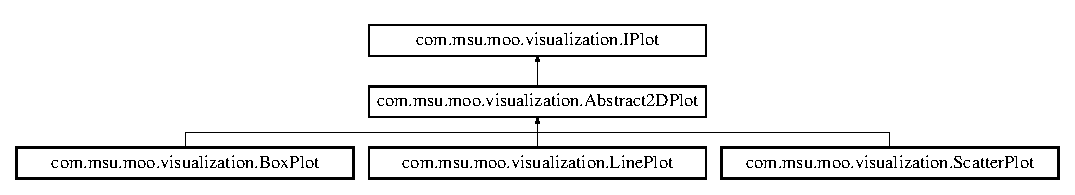
\includegraphics[height=2.178988cm]{classcom_1_1msu_1_1moo_1_1visualization_1_1Abstract2DPlot}
\end{center}
\end{figure}
\subsection*{Public Member Functions}
\begin{DoxyCompactItemize}
\item 
\hypertarget{classcom_1_1msu_1_1moo_1_1visualization_1_1Abstract2DPlot_af20d6a02952b9b49e4b44f98a2855dc3}{{\bfseries Abstract2\-D\-Plot} (String title)}\label{classcom_1_1msu_1_1moo_1_1visualization_1_1Abstract2DPlot_af20d6a02952b9b49e4b44f98a2855dc3}

\item 
\hypertarget{classcom_1_1msu_1_1moo_1_1visualization_1_1Abstract2DPlot_af5135db46cd94a13fcd97473e62651ac}{{\bfseries Abstract2\-D\-Plot} (String title, String x\-Label, String y\-Label)}\label{classcom_1_1msu_1_1moo_1_1visualization_1_1Abstract2DPlot_af5135db46cd94a13fcd97473e62651ac}

\item 
\hypertarget{classcom_1_1msu_1_1moo_1_1visualization_1_1Abstract2DPlot_a1b2666e725e73d52d01928fbc129b189}{void {\bfseries save} (String name)}\label{classcom_1_1msu_1_1moo_1_1visualization_1_1Abstract2DPlot_a1b2666e725e73d52d01928fbc129b189}

\item 
\hypertarget{classcom_1_1msu_1_1moo_1_1visualization_1_1Abstract2DPlot_a75fa89c65b4a3c5e71cccf5fd9c39286}{void {\bfseries show} ()}\label{classcom_1_1msu_1_1moo_1_1visualization_1_1Abstract2DPlot_a75fa89c65b4a3c5e71cccf5fd9c39286}

\end{DoxyCompactItemize}
\subsection*{Protected Attributes}
\begin{DoxyCompactItemize}
\item 
\hypertarget{classcom_1_1msu_1_1moo_1_1visualization_1_1Abstract2DPlot_ac147640f3cb063905aa1e197d3bef23a}{String {\bfseries title} = \char`\"{}Title\char`\"{}}\label{classcom_1_1msu_1_1moo_1_1visualization_1_1Abstract2DPlot_ac147640f3cb063905aa1e197d3bef23a}

\item 
\hypertarget{classcom_1_1msu_1_1moo_1_1visualization_1_1Abstract2DPlot_ac7d30afeecc28908074b9acb0dee7fba}{String {\bfseries x\-Label} = \char`\"{}X\char`\"{}}\label{classcom_1_1msu_1_1moo_1_1visualization_1_1Abstract2DPlot_ac7d30afeecc28908074b9acb0dee7fba}

\item 
\hypertarget{classcom_1_1msu_1_1moo_1_1visualization_1_1Abstract2DPlot_a7c1266b57c84433f3a56a1b29c7956b9}{String {\bfseries y\-Label} = \char`\"{}Y\char`\"{}}\label{classcom_1_1msu_1_1moo_1_1visualization_1_1Abstract2DPlot_a7c1266b57c84433f3a56a1b29c7956b9}

\end{DoxyCompactItemize}


The documentation for this class was generated from the following file\-:\begin{DoxyCompactItemize}
\item 
src/main/java/com/msu/moo/visualization/Abstract2\-D\-Plot.\-java\end{DoxyCompactItemize}

\hypertarget{classcom_1_1msu_1_1moo_1_1model_1_1AbstractAlgorithm_3_01V_01extends_01IVariable_00_01P_01extends_01IProblem_01_4}{\section{com.\-msu.\-moo.\-model.\-Abstract\-Algorithm$<$ V extends I\-Variable, P extends I\-Problem $>$ Class Reference}
\label{classcom_1_1msu_1_1moo_1_1model_1_1AbstractAlgorithm_3_01V_01extends_01IVariable_00_01P_01extends_01IProblem_01_4}\index{com.\-msu.\-moo.\-model.\-Abstract\-Algorithm$<$ V extends I\-Variable, P extends I\-Problem $>$@{com.\-msu.\-moo.\-model.\-Abstract\-Algorithm$<$ V extends I\-Variable, P extends I\-Problem $>$}}
}
Inheritance diagram for com.\-msu.\-moo.\-model.\-Abstract\-Algorithm$<$ V extends I\-Variable, P extends I\-Problem $>$\-:\begin{figure}[H]
\begin{center}
\leavevmode
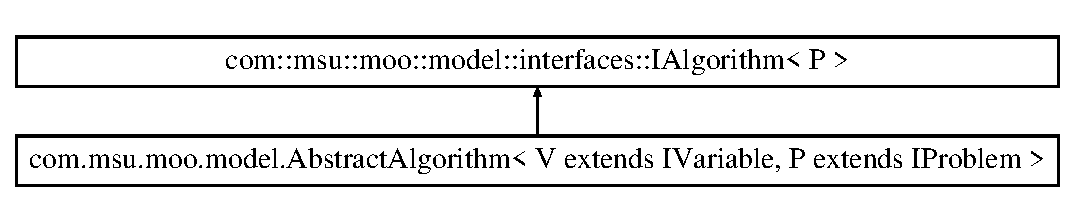
\includegraphics[height=2.000000cm]{classcom_1_1msu_1_1moo_1_1model_1_1AbstractAlgorithm_3_01V_01extends_01IVariable_00_01P_01extends_01IProblem_01_4}
\end{center}
\end{figure}
\subsection*{Public Member Functions}
\begin{DoxyCompactItemize}
\item 
\hypertarget{classcom_1_1msu_1_1moo_1_1model_1_1AbstractAlgorithm_3_01V_01extends_01IVariable_00_01P_01extends_01IProblem_01_4_a51d41c295a949704b82208e9c48500f6}{{\bfseries Abstract\-Algorithm} (Variable\-Factory$<$ V, P $>$ factory)}\label{classcom_1_1msu_1_1moo_1_1model_1_1AbstractAlgorithm_3_01V_01extends_01IVariable_00_01P_01extends_01IProblem_01_4_a51d41c295a949704b82208e9c48500f6}

\item 
\hypertarget{classcom_1_1msu_1_1moo_1_1model_1_1AbstractAlgorithm_3_01V_01extends_01IVariable_00_01P_01extends_01IProblem_01_4_ae2ece446048281cbb3c241df4bd85f22}{\hyperlink{classcom_1_1msu_1_1moo_1_1model_1_1solution_1_1NonDominatedSolutionSet}{Non\-Dominated\-Solution\-Set} {\bfseries run} (P \hyperlink{classcom_1_1msu_1_1moo_1_1model_1_1AbstractAlgorithm_3_01V_01extends_01IVariable_00_01P_01extends_01IProblem_01_4_a0fe30f89d43d13046d955b5cd2ce2cfb}{problem})}\label{classcom_1_1msu_1_1moo_1_1model_1_1AbstractAlgorithm_3_01V_01extends_01IVariable_00_01P_01extends_01IProblem_01_4_ae2ece446048281cbb3c241df4bd85f22}

\item 
\hypertarget{classcom_1_1msu_1_1moo_1_1model_1_1AbstractAlgorithm_3_01V_01extends_01IVariable_00_01P_01extends_01IProblem_01_4_a97f9e8061a47943916f87759c9ef2223}{boolean {\bfseries has\-Finished} ()}\label{classcom_1_1msu_1_1moo_1_1model_1_1AbstractAlgorithm_3_01V_01extends_01IVariable_00_01P_01extends_01IProblem_01_4_a97f9e8061a47943916f87759c9ef2223}

\item 
\hypertarget{classcom_1_1msu_1_1moo_1_1model_1_1AbstractAlgorithm_3_01V_01extends_01IVariable_00_01P_01extends_01IProblem_01_4_a1f063330fbdaba32f0085ee3bbc6753c}{void {\bfseries set\-Max\-Evaluations} (long n)}\label{classcom_1_1msu_1_1moo_1_1model_1_1AbstractAlgorithm_3_01V_01extends_01IVariable_00_01P_01extends_01IProblem_01_4_a1f063330fbdaba32f0085ee3bbc6753c}

\item 
\hypertarget{classcom_1_1msu_1_1moo_1_1model_1_1AbstractAlgorithm_3_01V_01extends_01IVariable_00_01P_01extends_01IProblem_01_4_ac646d823214bec2258910a440341daf0}{String {\bfseries get\-Name} ()}\label{classcom_1_1msu_1_1moo_1_1model_1_1AbstractAlgorithm_3_01V_01extends_01IVariable_00_01P_01extends_01IProblem_01_4_ac646d823214bec2258910a440341daf0}

\item 
\hypertarget{classcom_1_1msu_1_1moo_1_1model_1_1AbstractAlgorithm_3_01V_01extends_01IVariable_00_01P_01extends_01IProblem_01_4_ab7079d127af5c5c9781ad167f52add4b}{void {\bfseries set\-Name} (String name)}\label{classcom_1_1msu_1_1moo_1_1model_1_1AbstractAlgorithm_3_01V_01extends_01IVariable_00_01P_01extends_01IProblem_01_4_ab7079d127af5c5c9781ad167f52add4b}

\item 
\hypertarget{classcom_1_1msu_1_1moo_1_1model_1_1AbstractAlgorithm_3_01V_01extends_01IVariable_00_01P_01extends_01IProblem_01_4_a1d2933c112754b006c84a0377c136cc9}{String {\bfseries to\-String} ()}\label{classcom_1_1msu_1_1moo_1_1model_1_1AbstractAlgorithm_3_01V_01extends_01IVariable_00_01P_01extends_01IProblem_01_4_a1d2933c112754b006c84a0377c136cc9}

\item 
\hypertarget{classcom_1_1msu_1_1moo_1_1model_1_1AbstractAlgorithm_3_01V_01extends_01IVariable_00_01P_01extends_01IProblem_01_4_a3522c7a9db62a1fcfd9454472467d0b8}{Variable\-Factory$<$ V, P $>$ {\bfseries get\-Factory} ()}\label{classcom_1_1msu_1_1moo_1_1model_1_1AbstractAlgorithm_3_01V_01extends_01IVariable_00_01P_01extends_01IProblem_01_4_a3522c7a9db62a1fcfd9454472467d0b8}

\item 
\hypertarget{classcom_1_1msu_1_1moo_1_1model_1_1AbstractAlgorithm_3_01V_01extends_01IVariable_00_01P_01extends_01IProblem_01_4_ae65899825c221aa6a991dc327793b5d8}{void {\bfseries set\-Factory} (Variable\-Factory$<$ V, P $>$ factory)}\label{classcom_1_1msu_1_1moo_1_1model_1_1AbstractAlgorithm_3_01V_01extends_01IVariable_00_01P_01extends_01IProblem_01_4_ae65899825c221aa6a991dc327793b5d8}

\item 
\hypertarget{classcom_1_1msu_1_1moo_1_1model_1_1AbstractAlgorithm_3_01V_01extends_01IVariable_00_01P_01extends_01IProblem_01_4_ac9b5c48530b0df0ae4cab8299ba5bb96}{long {\bfseries get\-Max\-Evaluations} ()}\label{classcom_1_1msu_1_1moo_1_1model_1_1AbstractAlgorithm_3_01V_01extends_01IVariable_00_01P_01extends_01IProblem_01_4_ac9b5c48530b0df0ae4cab8299ba5bb96}

\item 
\hypertarget{classcom_1_1msu_1_1moo_1_1model_1_1AbstractAlgorithm_3_01V_01extends_01IVariable_00_01P_01extends_01IProblem_01_4_ad2d50c30de2a644c56ae7cc3bbbb695d}{Map$<$ Long, \\*
\hyperlink{classcom_1_1msu_1_1moo_1_1model_1_1solution_1_1NonDominatedSolutionSet}{Non\-Dominated\-Solution\-Set} $>$ {\bfseries get\-History} ()}\label{classcom_1_1msu_1_1moo_1_1model_1_1AbstractAlgorithm_3_01V_01extends_01IVariable_00_01P_01extends_01IProblem_01_4_ad2d50c30de2a644c56ae7cc3bbbb695d}

\end{DoxyCompactItemize}
\subsection*{Protected Member Functions}
\begin{DoxyCompactItemize}
\item 
\hypertarget{classcom_1_1msu_1_1moo_1_1model_1_1AbstractAlgorithm_3_01V_01extends_01IVariable_00_01P_01extends_01IProblem_01_4_a0b87e611c820dcc7b34b9b91b15b0714}{abstract void {\bfseries initialize} ()}\label{classcom_1_1msu_1_1moo_1_1model_1_1AbstractAlgorithm_3_01V_01extends_01IVariable_00_01P_01extends_01IProblem_01_4_a0b87e611c820dcc7b34b9b91b15b0714}

\item 
\hypertarget{classcom_1_1msu_1_1moo_1_1model_1_1AbstractAlgorithm_3_01V_01extends_01IVariable_00_01P_01extends_01IProblem_01_4_a49e9ac6000131b2036ed08b579754a47}{abstract void {\bfseries next} ()}\label{classcom_1_1msu_1_1moo_1_1model_1_1AbstractAlgorithm_3_01V_01extends_01IVariable_00_01P_01extends_01IProblem_01_4_a49e9ac6000131b2036ed08b579754a47}

\item 
\hypertarget{classcom_1_1msu_1_1moo_1_1model_1_1AbstractAlgorithm_3_01V_01extends_01IVariable_00_01P_01extends_01IProblem_01_4_a0c4ee488b21a671a897eda4a999d4246}{abstract \hyperlink{classcom_1_1msu_1_1moo_1_1model_1_1solution_1_1NonDominatedSolutionSet}{Non\-Dominated\-Solution\-Set} \hyperlink{classcom_1_1msu_1_1moo_1_1model_1_1AbstractAlgorithm_3_01V_01extends_01IVariable_00_01P_01extends_01IProblem_01_4_a0c4ee488b21a671a897eda4a999d4246}{get\-Result} ()}\label{classcom_1_1msu_1_1moo_1_1model_1_1AbstractAlgorithm_3_01V_01extends_01IVariable_00_01P_01extends_01IProblem_01_4_a0c4ee488b21a671a897eda4a999d4246}

\begin{DoxyCompactList}\small\item\em return the front as a result -\/$>$ should be available every generation \end{DoxyCompactList}\end{DoxyCompactItemize}
\subsection*{Protected Attributes}
\begin{DoxyCompactItemize}
\item 
\hypertarget{classcom_1_1msu_1_1moo_1_1model_1_1AbstractAlgorithm_3_01V_01extends_01IVariable_00_01P_01extends_01IProblem_01_4_a0fe30f89d43d13046d955b5cd2ce2cfb}{P \hyperlink{classcom_1_1msu_1_1moo_1_1model_1_1AbstractAlgorithm_3_01V_01extends_01IVariable_00_01P_01extends_01IProblem_01_4_a0fe30f89d43d13046d955b5cd2ce2cfb}{problem} = null}\label{classcom_1_1msu_1_1moo_1_1model_1_1AbstractAlgorithm_3_01V_01extends_01IVariable_00_01P_01extends_01IProblem_01_4_a0fe30f89d43d13046d955b5cd2ce2cfb}

\begin{DoxyCompactList}\small\item\em the current problem \end{DoxyCompactList}\item 
\hypertarget{classcom_1_1msu_1_1moo_1_1model_1_1AbstractAlgorithm_3_01V_01extends_01IVariable_00_01P_01extends_01IProblem_01_4_a1cd991b70748d61c6eca9779d8cba8bb}{Variable\-Factory$<$ V, P $>$ {\bfseries factory} = null}\label{classcom_1_1msu_1_1moo_1_1model_1_1AbstractAlgorithm_3_01V_01extends_01IVariable_00_01P_01extends_01IProblem_01_4_a1cd991b70748d61c6eca9779d8cba8bb}

\item 
\hypertarget{classcom_1_1msu_1_1moo_1_1model_1_1AbstractAlgorithm_3_01V_01extends_01IVariable_00_01P_01extends_01IProblem_01_4_a60dfcbe7207238835d637128c2a234fa}{long {\bfseries max\-Evaluations} = 50000\-L}\label{classcom_1_1msu_1_1moo_1_1model_1_1AbstractAlgorithm_3_01V_01extends_01IVariable_00_01P_01extends_01IProblem_01_4_a60dfcbe7207238835d637128c2a234fa}

\item 
\hypertarget{classcom_1_1msu_1_1moo_1_1model_1_1AbstractAlgorithm_3_01V_01extends_01IVariable_00_01P_01extends_01IProblem_01_4_a31eed2b6e932ca5085e7fd126866ce60}{String {\bfseries name} = get\-Class().get\-Simple\-Name()}\label{classcom_1_1msu_1_1moo_1_1model_1_1AbstractAlgorithm_3_01V_01extends_01IVariable_00_01P_01extends_01IProblem_01_4_a31eed2b6e932ca5085e7fd126866ce60}

\item 
\hypertarget{classcom_1_1msu_1_1moo_1_1model_1_1AbstractAlgorithm_3_01V_01extends_01IVariable_00_01P_01extends_01IProblem_01_4_a99eccfca17f5dd0685d385cab0e87bc2}{boolean {\bfseries record\-History} = true}\label{classcom_1_1msu_1_1moo_1_1model_1_1AbstractAlgorithm_3_01V_01extends_01IVariable_00_01P_01extends_01IProblem_01_4_a99eccfca17f5dd0685d385cab0e87bc2}

\item 
\hypertarget{classcom_1_1msu_1_1moo_1_1model_1_1AbstractAlgorithm_3_01V_01extends_01IVariable_00_01P_01extends_01IProblem_01_4_aea4d1c1dd0ff1ae33abef984402d1529}{Map$<$ Long, \\*
\hyperlink{classcom_1_1msu_1_1moo_1_1model_1_1solution_1_1NonDominatedSolutionSet}{Non\-Dominated\-Solution\-Set} $>$ {\bfseries history} = new Tree\-Map$<$$>$()}\label{classcom_1_1msu_1_1moo_1_1model_1_1AbstractAlgorithm_3_01V_01extends_01IVariable_00_01P_01extends_01IProblem_01_4_aea4d1c1dd0ff1ae33abef984402d1529}

\end{DoxyCompactItemize}


The documentation for this class was generated from the following file\-:\begin{DoxyCompactItemize}
\item 
src/main/java/com/msu/moo/model/Abstract\-Algorithm.\-java\end{DoxyCompactItemize}

\hypertarget{classcom_1_1msu_1_1moo_1_1operators_1_1AbstractCrossover_3_01T_01_4}{\section{com.\-msu.\-moo.\-operators.\-Abstract\-Crossover$<$ T $>$ Class Reference}
\label{classcom_1_1msu_1_1moo_1_1operators_1_1AbstractCrossover_3_01T_01_4}\index{com.\-msu.\-moo.\-operators.\-Abstract\-Crossover$<$ T $>$@{com.\-msu.\-moo.\-operators.\-Abstract\-Crossover$<$ T $>$}}
}
\subsection*{Public Member Functions}
\begin{DoxyCompactItemize}
\item 
\hypertarget{classcom_1_1msu_1_1moo_1_1operators_1_1AbstractCrossover_3_01T_01_4_a8b517aa8452e5962e751af3392b79538}{List$<$ \hyperlink{interfacecom_1_1msu_1_1moo_1_1model_1_1interfaces_1_1IVariable}{I\-Variable} $>$ {\bfseries crossover} (\hyperlink{interfacecom_1_1msu_1_1moo_1_1model_1_1interfaces_1_1IVariable}{I\-Variable} a, \hyperlink{interfacecom_1_1msu_1_1moo_1_1model_1_1interfaces_1_1IVariable}{I\-Variable} b)}\label{classcom_1_1msu_1_1moo_1_1operators_1_1AbstractCrossover_3_01T_01_4_a8b517aa8452e5962e751af3392b79538}

\end{DoxyCompactItemize}
\subsection*{Protected Member Functions}
\begin{DoxyCompactItemize}
\item 
\hypertarget{classcom_1_1msu_1_1moo_1_1operators_1_1AbstractCrossover_3_01T_01_4_a2e78a307f6c18698927da579acdfbfbf}{abstract List$<$ T $>$ {\bfseries crossover\-\_\-} (T a, T b)}\label{classcom_1_1msu_1_1moo_1_1operators_1_1AbstractCrossover_3_01T_01_4_a2e78a307f6c18698927da579acdfbfbf}

\end{DoxyCompactItemize}


\subsection{Detailed Description}
This is an abstract Crossover of an object. This class which inherits from this one could specify which type is expected to be used to crossover. Otherwise there will be an error thrown.


\begin{DoxyParams}{Parameters}
{\em $<$\-T$>$} & type which could be mutated! \\
\hline
\end{DoxyParams}


The documentation for this class was generated from the following file\-:\begin{DoxyCompactItemize}
\item 
src/main/java/com/msu/moo/operators/Abstract\-Crossover.\-java\end{DoxyCompactItemize}

\hypertarget{classcom_1_1msu_1_1moo_1_1experiment_1_1AbstractExperiment_3_01P_01extends_01IProblem_01_4}{\section{com.\-msu.\-moo.\-experiment.\-Abstract\-Experiment$<$ P extends I\-Problem $>$ Class Reference}
\label{classcom_1_1msu_1_1moo_1_1experiment_1_1AbstractExperiment_3_01P_01extends_01IProblem_01_4}\index{com.\-msu.\-moo.\-experiment.\-Abstract\-Experiment$<$ P extends I\-Problem $>$@{com.\-msu.\-moo.\-experiment.\-Abstract\-Experiment$<$ P extends I\-Problem $>$}}
}
\subsection*{Public Member Functions}
\begin{DoxyCompactItemize}
\item 
\hypertarget{classcom_1_1msu_1_1moo_1_1experiment_1_1AbstractExperiment_3_01P_01extends_01IProblem_01_4_a6da0cc245c9ec4eff288b73fdff8a4c9}{abstract void {\bfseries report} ()}\label{classcom_1_1msu_1_1moo_1_1experiment_1_1AbstractExperiment_3_01P_01extends_01IProblem_01_4_a6da0cc245c9ec4eff288b73fdff8a4c9}

\item 
\hypertarget{classcom_1_1msu_1_1moo_1_1experiment_1_1AbstractExperiment_3_01P_01extends_01IProblem_01_4_a56a01b557b3f59d10a1f22659882b705}{void {\bfseries run} (long max\-Evaluations, int iterations, long seed)}\label{classcom_1_1msu_1_1moo_1_1experiment_1_1AbstractExperiment_3_01P_01extends_01IProblem_01_4_a56a01b557b3f59d10a1f22659882b705}

\item 
\hyperlink{classcom_1_1msu_1_1moo_1_1experiment_1_1ExperimentResult}{Experiment\-Result} \hyperlink{classcom_1_1msu_1_1moo_1_1experiment_1_1AbstractExperiment_3_01P_01extends_01IProblem_01_4_ade7890252c0b9e5e523d5c19b289dbb0}{get\-Result} ()
\end{DoxyCompactItemize}
\subsection*{Static Public Member Functions}
\begin{DoxyCompactItemize}
\item 
\hypertarget{classcom_1_1msu_1_1moo_1_1experiment_1_1AbstractExperiment_3_01P_01extends_01IProblem_01_4_a8096c2b69a833a9692726e14dda9bc6e}{static \hyperlink{classcom_1_1msu_1_1moo_1_1model_1_1solution_1_1NonDominatedSolutionSet}{Non\-Dominated\-Solution\-Set} {\bfseries estimate\-True\-Front} (Collection$<$ \hyperlink{classcom_1_1msu_1_1moo_1_1model_1_1solution_1_1NonDominatedSolutionSet}{Non\-Dominated\-Solution\-Set} $>$ sets)}\label{classcom_1_1msu_1_1moo_1_1experiment_1_1AbstractExperiment_3_01P_01extends_01IProblem_01_4_a8096c2b69a833a9692726e14dda9bc6e}

\end{DoxyCompactItemize}
\subsection*{Protected Member Functions}
\begin{DoxyCompactItemize}
\item 
\hypertarget{classcom_1_1msu_1_1moo_1_1experiment_1_1AbstractExperiment_3_01P_01extends_01IProblem_01_4_a9eeddd6dff34d9f11b4391ba1e5f7ee7}{abstract List$<$ I\-Algorithm$<$ P $>$ $>$ {\bfseries get\-Algorithms} ()}\label{classcom_1_1msu_1_1moo_1_1experiment_1_1AbstractExperiment_3_01P_01extends_01IProblem_01_4_a9eeddd6dff34d9f11b4391ba1e5f7ee7}

\item 
\hypertarget{classcom_1_1msu_1_1moo_1_1experiment_1_1AbstractExperiment_3_01P_01extends_01IProblem_01_4_a234b093f07b1ef31305979f1ffb8ca58}{abstract Map$<$ P, \\*
\hyperlink{classcom_1_1msu_1_1moo_1_1model_1_1solution_1_1NonDominatedSolutionSet}{Non\-Dominated\-Solution\-Set} $>$ {\bfseries get\-Problems} ()}\label{classcom_1_1msu_1_1moo_1_1experiment_1_1AbstractExperiment_3_01P_01extends_01IProblem_01_4_a234b093f07b1ef31305979f1ffb8ca58}

\end{DoxyCompactItemize}
\subsection*{Protected Attributes}
\begin{DoxyCompactItemize}
\item 
\hypertarget{classcom_1_1msu_1_1moo_1_1experiment_1_1AbstractExperiment_3_01P_01extends_01IProblem_01_4_a6fbedc4936842a96644da8c9692f8721}{List$<$ I\-Algorithm$<$ P $>$ $>$ {\bfseries algorithms} = null}\label{classcom_1_1msu_1_1moo_1_1experiment_1_1AbstractExperiment_3_01P_01extends_01IProblem_01_4_a6fbedc4936842a96644da8c9692f8721}

\item 
\hypertarget{classcom_1_1msu_1_1moo_1_1experiment_1_1AbstractExperiment_3_01P_01extends_01IProblem_01_4_adb67884bef8f5afcf5c1679834cd5158}{Map$<$ P, \hyperlink{classcom_1_1msu_1_1moo_1_1model_1_1solution_1_1NonDominatedSolutionSet}{Non\-Dominated\-Solution\-Set} $>$ {\bfseries problems} = null}\label{classcom_1_1msu_1_1moo_1_1experiment_1_1AbstractExperiment_3_01P_01extends_01IProblem_01_4_adb67884bef8f5afcf5c1679834cd5158}

\item 
\hypertarget{classcom_1_1msu_1_1moo_1_1experiment_1_1AbstractExperiment_3_01P_01extends_01IProblem_01_4_a58c7d7d29537684f275d2e27c5edd7bb}{\hyperlink{classcom_1_1msu_1_1moo_1_1experiment_1_1ExperimentResult}{Experiment\-Result} {\bfseries exp\-Result} = null}\label{classcom_1_1msu_1_1moo_1_1experiment_1_1AbstractExperiment_3_01P_01extends_01IProblem_01_4_a58c7d7d29537684f275d2e27c5edd7bb}

\end{DoxyCompactItemize}


\subsection{Member Function Documentation}
\hypertarget{classcom_1_1msu_1_1moo_1_1experiment_1_1AbstractExperiment_3_01P_01extends_01IProblem_01_4_ade7890252c0b9e5e523d5c19b289dbb0}{\index{com\-::msu\-::moo\-::experiment\-::\-Abstract\-Experiment$<$ P extends I\-Problem $>$@{com\-::msu\-::moo\-::experiment\-::\-Abstract\-Experiment$<$ P extends I\-Problem $>$}!get\-Result@{get\-Result}}
\index{get\-Result@{get\-Result}!com::msu::moo::experiment::AbstractExperiment< P extends IProblem >@{com\-::msu\-::moo\-::experiment\-::\-Abstract\-Experiment$<$ P extends I\-Problem $>$}}
\subsubsection[{get\-Result}]{\setlength{\rightskip}{0pt plus 5cm}{\bf Experiment\-Result} com.\-msu.\-moo.\-experiment.\-Abstract\-Experiment$<$ P extends {\bf I\-Problem} $>$.get\-Result (
\begin{DoxyParamCaption}
{}
\end{DoxyParamCaption}
)\hspace{0.3cm}{\ttfamily [inline]}}}\label{classcom_1_1msu_1_1moo_1_1experiment_1_1AbstractExperiment_3_01P_01extends_01IProblem_01_4_ade7890252c0b9e5e523d5c19b289dbb0}
\begin{DoxyReturn}{Returns}
the result of the experiment. if not executed it will be null. 
\end{DoxyReturn}


The documentation for this class was generated from the following file\-:\begin{DoxyCompactItemize}
\item 
src/main/java/com/msu/moo/experiment/Abstract\-Experiment.\-java\end{DoxyCompactItemize}

\hypertarget{classcom_1_1msu_1_1moo_1_1operators_1_1AbstractListCrossover_3_01T_01_4}{\section{com.\-msu.\-moo.\-operators.\-Abstract\-List\-Crossover$<$ T $>$ Class Reference}
\label{classcom_1_1msu_1_1moo_1_1operators_1_1AbstractListCrossover_3_01T_01_4}\index{com.\-msu.\-moo.\-operators.\-Abstract\-List\-Crossover$<$ T $>$@{com.\-msu.\-moo.\-operators.\-Abstract\-List\-Crossover$<$ T $>$}}
}
Inheritance diagram for com.\-msu.\-moo.\-operators.\-Abstract\-List\-Crossover$<$ T $>$\-:\begin{figure}[H]
\begin{center}
\leavevmode
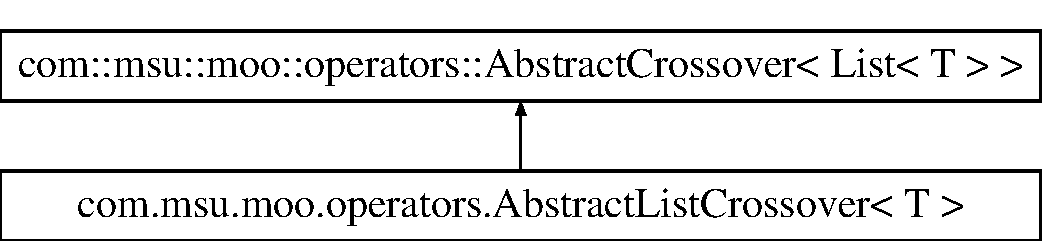
\includegraphics[height=2.000000cm]{classcom_1_1msu_1_1moo_1_1operators_1_1AbstractListCrossover_3_01T_01_4}
\end{center}
\end{figure}
\subsection*{Protected Member Functions}
\begin{DoxyCompactItemize}
\item 
\hypertarget{classcom_1_1msu_1_1moo_1_1operators_1_1AbstractListCrossover_3_01T_01_4_a3ef3d15e49fe5d5a6ffa7488c2d39a34}{List$<$ List$<$ T $>$ $>$ {\bfseries crossover\-\_\-} (List$<$ T $>$ a, List$<$ T $>$ b)}\label{classcom_1_1msu_1_1moo_1_1operators_1_1AbstractListCrossover_3_01T_01_4_a3ef3d15e49fe5d5a6ffa7488c2d39a34}

\item 
\hypertarget{classcom_1_1msu_1_1moo_1_1operators_1_1AbstractListCrossover_3_01T_01_4_aa6507d9fbe91745b023ec164d341e767}{abstract List$<$ List$<$ T $>$ $>$ {\bfseries crossover\-Lists} (List$<$ T $>$ a, List$<$ T $>$ b)}\label{classcom_1_1msu_1_1moo_1_1operators_1_1AbstractListCrossover_3_01T_01_4_aa6507d9fbe91745b023ec164d341e767}

\end{DoxyCompactItemize}


The documentation for this class was generated from the following file\-:\begin{DoxyCompactItemize}
\item 
src/main/java/com/msu/moo/operators/Abstract\-List\-Crossover.\-java\end{DoxyCompactItemize}

\hypertarget{classcom_1_1msu_1_1moo_1_1operators_1_1AbstractMutation_3_01T_01_4}{\section{com.\-msu.\-moo.\-operators.\-Abstract\-Mutation$<$ T $>$ Class Reference}
\label{classcom_1_1msu_1_1moo_1_1operators_1_1AbstractMutation_3_01T_01_4}\index{com.\-msu.\-moo.\-operators.\-Abstract\-Mutation$<$ T $>$@{com.\-msu.\-moo.\-operators.\-Abstract\-Mutation$<$ T $>$}}
}
\subsection*{Public Member Functions}
\begin{DoxyCompactItemize}
\item 
\hypertarget{classcom_1_1msu_1_1moo_1_1operators_1_1AbstractMutation_3_01T_01_4_a71b24427e5e7a377893158d84ad69179}{\hyperlink{interfacecom_1_1msu_1_1moo_1_1model_1_1interfaces_1_1IVariable}{I\-Variable} {\bfseries mutate} (\hyperlink{interfacecom_1_1msu_1_1moo_1_1model_1_1interfaces_1_1IVariable}{I\-Variable} a)}\label{classcom_1_1msu_1_1moo_1_1operators_1_1AbstractMutation_3_01T_01_4_a71b24427e5e7a377893158d84ad69179}

\end{DoxyCompactItemize}
\subsection*{Protected Member Functions}
\begin{DoxyCompactItemize}
\item 
\hypertarget{classcom_1_1msu_1_1moo_1_1operators_1_1AbstractMutation_3_01T_01_4_a91fc93fc85d9b67767545fd6490d0fc0}{abstract void {\bfseries mutate\-\_\-} (T element)}\label{classcom_1_1msu_1_1moo_1_1operators_1_1AbstractMutation_3_01T_01_4_a91fc93fc85d9b67767545fd6490d0fc0}

\end{DoxyCompactItemize}


\subsection{Detailed Description}
This is an abstract Mutation of an object. This class which inherits from this one could specify which type is expected to mutate. Otherwise there will be an error thrown.


\begin{DoxyParams}{Parameters}
{\em $<$\-T$>$} & type which could be mutated! \\
\hline
\end{DoxyParams}


The documentation for this class was generated from the following file\-:\begin{DoxyCompactItemize}
\item 
src/main/java/com/msu/moo/operators/Abstract\-Mutation.\-java\end{DoxyCompactItemize}

\hypertarget{classcom_1_1msu_1_1moo_1_1model_1_1AbstractProblem_3_01V_01extends_01IVariable_01_4}{\section{com.\-msu.\-moo.\-model.\-Abstract\-Problem$<$ V extends I\-Variable $>$ Class Reference}
\label{classcom_1_1msu_1_1moo_1_1model_1_1AbstractProblem_3_01V_01extends_01IVariable_01_4}\index{com.\-msu.\-moo.\-model.\-Abstract\-Problem$<$ V extends I\-Variable $>$@{com.\-msu.\-moo.\-model.\-Abstract\-Problem$<$ V extends I\-Variable $>$}}
}
Inheritance diagram for com.\-msu.\-moo.\-model.\-Abstract\-Problem$<$ V extends I\-Variable $>$\-:\begin{figure}[H]
\begin{center}
\leavevmode
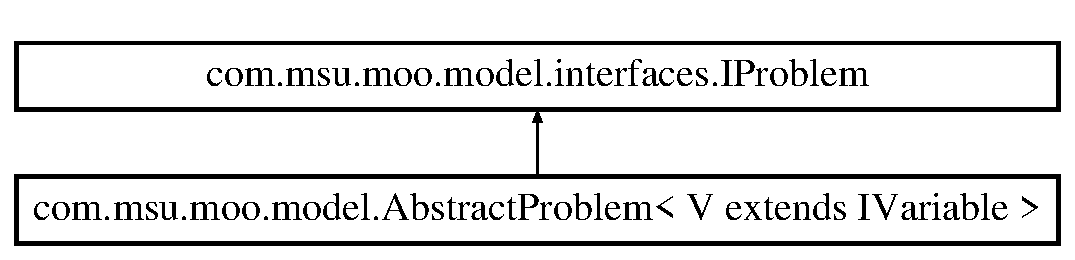
\includegraphics[height=2.000000cm]{classcom_1_1msu_1_1moo_1_1model_1_1AbstractProblem_3_01V_01extends_01IVariable_01_4}
\end{center}
\end{figure}
\subsection*{Public Member Functions}
\begin{DoxyCompactItemize}
\item 
long \hyperlink{classcom_1_1msu_1_1moo_1_1model_1_1AbstractProblem_3_01V_01extends_01IVariable_01_4_a6d774087779671d0478dcc5beb25c7b9}{get\-Num\-Of\-Evaluations} ()
\item 
void \hyperlink{classcom_1_1msu_1_1moo_1_1model_1_1AbstractProblem_3_01V_01extends_01IVariable_01_4_ae3d2d54f9ada94985968dc96a03d22df}{reset} ()
\item 
\hyperlink{classcom_1_1msu_1_1moo_1_1model_1_1solution_1_1Solution}{Solution} \hyperlink{classcom_1_1msu_1_1moo_1_1model_1_1AbstractProblem_3_01V_01extends_01IVariable_01_4_a9ed0a86fb3bb92cda13cd331013dcc00}{evaluate} (\hyperlink{interfacecom_1_1msu_1_1moo_1_1model_1_1interfaces_1_1IVariable}{I\-Variable} variable)
\item 
\hypertarget{classcom_1_1msu_1_1moo_1_1model_1_1AbstractProblem_3_01V_01extends_01IVariable_01_4_a5574c3ea3a28a568915c01ca05e8f01d}{String {\bfseries to\-String} ()}\label{classcom_1_1msu_1_1moo_1_1model_1_1AbstractProblem_3_01V_01extends_01IVariable_01_4_a5574c3ea3a28a568915c01ca05e8f01d}

\end{DoxyCompactItemize}
\subsection*{Protected Member Functions}
\begin{DoxyCompactItemize}
\item 
abstract List$<$ Double $>$ \hyperlink{classcom_1_1msu_1_1moo_1_1model_1_1AbstractProblem_3_01V_01extends_01IVariable_01_4_ae71651f19f19117959d846be540d9331}{evaluate\-\_\-} (V variable)
\end{DoxyCompactItemize}
\subsection*{Protected Attributes}
\begin{DoxyCompactItemize}
\item 
\hypertarget{classcom_1_1msu_1_1moo_1_1model_1_1AbstractProblem_3_01V_01extends_01IVariable_01_4_a55efd9266ee5e7e6affa618ba532e7ce}{long {\bfseries num\-Of\-Evaluations} = 0}\label{classcom_1_1msu_1_1moo_1_1model_1_1AbstractProblem_3_01V_01extends_01IVariable_01_4_a55efd9266ee5e7e6affa618ba532e7ce}

\end{DoxyCompactItemize}


\subsection{Member Function Documentation}
\hypertarget{classcom_1_1msu_1_1moo_1_1model_1_1AbstractProblem_3_01V_01extends_01IVariable_01_4_a9ed0a86fb3bb92cda13cd331013dcc00}{\index{com\-::msu\-::moo\-::model\-::\-Abstract\-Problem$<$ V extends I\-Variable $>$@{com\-::msu\-::moo\-::model\-::\-Abstract\-Problem$<$ V extends I\-Variable $>$}!evaluate@{evaluate}}
\index{evaluate@{evaluate}!com::msu::moo::model::AbstractProblem< V extends IVariable >@{com\-::msu\-::moo\-::model\-::\-Abstract\-Problem$<$ V extends I\-Variable $>$}}
\subsubsection[{evaluate}]{\setlength{\rightskip}{0pt plus 5cm}{\bf Solution} com.\-msu.\-moo.\-model.\-Abstract\-Problem$<$ V extends {\bf I\-Variable} $>$.evaluate (
\begin{DoxyParamCaption}
\item[{{\bf I\-Variable}}]{variable}
\end{DoxyParamCaption}
)\hspace{0.3cm}{\ttfamily [inline]}}}\label{classcom_1_1msu_1_1moo_1_1model_1_1AbstractProblem_3_01V_01extends_01IVariable_01_4_a9ed0a86fb3bb92cda13cd331013dcc00}
Returns the result of the problem according to the variable 
\begin{DoxyParams}{Parameters}
{\em variable} & extends I\-Variable and could be problem specific. \\
\hline
\end{DoxyParams}
\begin{DoxyReturn}{Returns}
Solution object which contains the result. 
\end{DoxyReturn}


Implements \hyperlink{interfacecom_1_1msu_1_1moo_1_1model_1_1interfaces_1_1IProblem_a1ac7c52476b19b10a1e167551b9ead19}{com.\-msu.\-moo.\-model.\-interfaces.\-I\-Problem}.

\hypertarget{classcom_1_1msu_1_1moo_1_1model_1_1AbstractProblem_3_01V_01extends_01IVariable_01_4_ae71651f19f19117959d846be540d9331}{\index{com\-::msu\-::moo\-::model\-::\-Abstract\-Problem$<$ V extends I\-Variable $>$@{com\-::msu\-::moo\-::model\-::\-Abstract\-Problem$<$ V extends I\-Variable $>$}!evaluate\-\_\-@{evaluate\-\_\-}}
\index{evaluate\-\_\-@{evaluate\-\_\-}!com::msu::moo::model::AbstractProblem< V extends IVariable >@{com\-::msu\-::moo\-::model\-::\-Abstract\-Problem$<$ V extends I\-Variable $>$}}
\subsubsection[{evaluate\-\_\-}]{\setlength{\rightskip}{0pt plus 5cm}abstract List$<$Double$>$ com.\-msu.\-moo.\-model.\-Abstract\-Problem$<$ V extends {\bf I\-Variable} $>$.evaluate\-\_\- (
\begin{DoxyParamCaption}
\item[{V}]{variable}
\end{DoxyParamCaption}
)\hspace{0.3cm}{\ttfamily [abstract]}, {\ttfamily [protected]}}}\label{classcom_1_1msu_1_1moo_1_1model_1_1AbstractProblem_3_01V_01extends_01IVariable_01_4_ae71651f19f19117959d846be540d9331}
Evaluation method that must be implemented by all subclasses. 
\begin{DoxyParams}{Parameters}
{\em variable} & input value \\
\hline
\end{DoxyParams}
\begin{DoxyReturn}{Returns}
objective results 
\end{DoxyReturn}
\hypertarget{classcom_1_1msu_1_1moo_1_1model_1_1AbstractProblem_3_01V_01extends_01IVariable_01_4_a6d774087779671d0478dcc5beb25c7b9}{\index{com\-::msu\-::moo\-::model\-::\-Abstract\-Problem$<$ V extends I\-Variable $>$@{com\-::msu\-::moo\-::model\-::\-Abstract\-Problem$<$ V extends I\-Variable $>$}!get\-Num\-Of\-Evaluations@{get\-Num\-Of\-Evaluations}}
\index{get\-Num\-Of\-Evaluations@{get\-Num\-Of\-Evaluations}!com::msu::moo::model::AbstractProblem< V extends IVariable >@{com\-::msu\-::moo\-::model\-::\-Abstract\-Problem$<$ V extends I\-Variable $>$}}
\subsubsection[{get\-Num\-Of\-Evaluations}]{\setlength{\rightskip}{0pt plus 5cm}long com.\-msu.\-moo.\-model.\-Abstract\-Problem$<$ V extends {\bf I\-Variable} $>$.get\-Num\-Of\-Evaluations (
\begin{DoxyParamCaption}
{}
\end{DoxyParamCaption}
)\hspace{0.3cm}{\ttfamily [inline]}}}\label{classcom_1_1msu_1_1moo_1_1model_1_1AbstractProblem_3_01V_01extends_01IVariable_01_4_a6d774087779671d0478dcc5beb25c7b9}
\begin{DoxyReturn}{Returns}
number of evaluations so far. 
\end{DoxyReturn}


Implements \hyperlink{interfacecom_1_1msu_1_1moo_1_1model_1_1interfaces_1_1IProblem_ad7dba60e3a3412017890543d3a0250b8}{com.\-msu.\-moo.\-model.\-interfaces.\-I\-Problem}.

\hypertarget{classcom_1_1msu_1_1moo_1_1model_1_1AbstractProblem_3_01V_01extends_01IVariable_01_4_ae3d2d54f9ada94985968dc96a03d22df}{\index{com\-::msu\-::moo\-::model\-::\-Abstract\-Problem$<$ V extends I\-Variable $>$@{com\-::msu\-::moo\-::model\-::\-Abstract\-Problem$<$ V extends I\-Variable $>$}!reset@{reset}}
\index{reset@{reset}!com::msu::moo::model::AbstractProblem< V extends IVariable >@{com\-::msu\-::moo\-::model\-::\-Abstract\-Problem$<$ V extends I\-Variable $>$}}
\subsubsection[{reset}]{\setlength{\rightskip}{0pt plus 5cm}void com.\-msu.\-moo.\-model.\-Abstract\-Problem$<$ V extends {\bf I\-Variable} $>$.reset (
\begin{DoxyParamCaption}
{}
\end{DoxyParamCaption}
)\hspace{0.3cm}{\ttfamily [inline]}}}\label{classcom_1_1msu_1_1moo_1_1model_1_1AbstractProblem_3_01V_01extends_01IVariable_01_4_ae3d2d54f9ada94985968dc96a03d22df}
Reset all evaluations, hashes and so on! 

Implements \hyperlink{interfacecom_1_1msu_1_1moo_1_1model_1_1interfaces_1_1IProblem_aca88ee486dcb7d96a218e76ea5034522}{com.\-msu.\-moo.\-model.\-interfaces.\-I\-Problem}.



The documentation for this class was generated from the following file\-:\begin{DoxyCompactItemize}
\item 
src/main/java/com/msu/moo/model/Abstract\-Problem.\-java\end{DoxyCompactItemize}

\hypertarget{classcom_1_1msu_1_1moo_1_1operators_1_1AbstractSelection}{\section{com.\-msu.\-moo.\-operators.\-Abstract\-Selection Class Reference}
\label{classcom_1_1msu_1_1moo_1_1operators_1_1AbstractSelection}\index{com.\-msu.\-moo.\-operators.\-Abstract\-Selection@{com.\-msu.\-moo.\-operators.\-Abstract\-Selection}}
}
Inheritance diagram for com.\-msu.\-moo.\-operators.\-Abstract\-Selection\-:\begin{figure}[H]
\begin{center}
\leavevmode
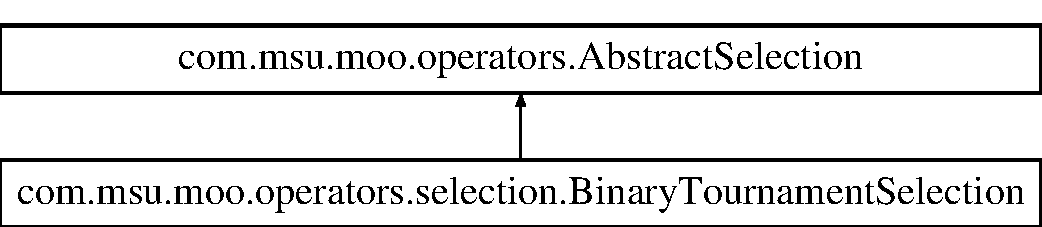
\includegraphics[height=2.000000cm]{classcom_1_1msu_1_1moo_1_1operators_1_1AbstractSelection}
\end{center}
\end{figure}
\subsection*{Public Member Functions}
\begin{DoxyCompactItemize}
\item 
\hypertarget{classcom_1_1msu_1_1moo_1_1operators_1_1AbstractSelection_aad5346960ec2e9d8c7d1b5068ed2ea49}{{\bfseries Abstract\-Selection} (\hyperlink{classcom_1_1msu_1_1moo_1_1model_1_1solution_1_1SolutionSet}{Solution\-Set} \hyperlink{classcom_1_1msu_1_1moo_1_1operators_1_1AbstractSelection_ade84bd57f9d26c9d9b2e90bb6591b79c}{set})}\label{classcom_1_1msu_1_1moo_1_1operators_1_1AbstractSelection_aad5346960ec2e9d8c7d1b5068ed2ea49}

\item 
abstract \hyperlink{classcom_1_1msu_1_1moo_1_1model_1_1solution_1_1Solution}{Solution} \hyperlink{classcom_1_1msu_1_1moo_1_1operators_1_1AbstractSelection_aa76e453252464eaca1d9337a41e4ade0}{next} ()
\item 
\hyperlink{classcom_1_1msu_1_1moo_1_1model_1_1solution_1_1SolutionSet}{Solution\-Set} \hyperlink{classcom_1_1msu_1_1moo_1_1operators_1_1AbstractSelection_a5b460b6d8320e9dd02fa8f12bd2e1e75}{next} (int n)
\end{DoxyCompactItemize}
\subsection*{Protected Attributes}
\begin{DoxyCompactItemize}
\item 
\hypertarget{classcom_1_1msu_1_1moo_1_1operators_1_1AbstractSelection_ade84bd57f9d26c9d9b2e90bb6591b79c}{\hyperlink{classcom_1_1msu_1_1moo_1_1model_1_1solution_1_1SolutionSet}{Solution\-Set} \hyperlink{classcom_1_1msu_1_1moo_1_1operators_1_1AbstractSelection_ade84bd57f9d26c9d9b2e90bb6591b79c}{set}}\label{classcom_1_1msu_1_1moo_1_1operators_1_1AbstractSelection_ade84bd57f9d26c9d9b2e90bb6591b79c}

\begin{DoxyCompactList}\small\item\em the solution set from which individuals will be selected \end{DoxyCompactList}\end{DoxyCompactItemize}


\subsection{Member Function Documentation}
\hypertarget{classcom_1_1msu_1_1moo_1_1operators_1_1AbstractSelection_aa76e453252464eaca1d9337a41e4ade0}{\index{com\-::msu\-::moo\-::operators\-::\-Abstract\-Selection@{com\-::msu\-::moo\-::operators\-::\-Abstract\-Selection}!next@{next}}
\index{next@{next}!com::msu::moo::operators::AbstractSelection@{com\-::msu\-::moo\-::operators\-::\-Abstract\-Selection}}
\subsubsection[{next}]{\setlength{\rightskip}{0pt plus 5cm}abstract {\bf Solution} com.\-msu.\-moo.\-operators.\-Abstract\-Selection.\-next (
\begin{DoxyParamCaption}
{}
\end{DoxyParamCaption}
)\hspace{0.3cm}{\ttfamily [abstract]}}}\label{classcom_1_1msu_1_1moo_1_1operators_1_1AbstractSelection_aa76e453252464eaca1d9337a41e4ade0}
\begin{DoxyReturn}{Returns}
next solution by selection implementation 
\end{DoxyReturn}
\hypertarget{classcom_1_1msu_1_1moo_1_1operators_1_1AbstractSelection_a5b460b6d8320e9dd02fa8f12bd2e1e75}{\index{com\-::msu\-::moo\-::operators\-::\-Abstract\-Selection@{com\-::msu\-::moo\-::operators\-::\-Abstract\-Selection}!next@{next}}
\index{next@{next}!com::msu::moo::operators::AbstractSelection@{com\-::msu\-::moo\-::operators\-::\-Abstract\-Selection}}
\subsubsection[{next}]{\setlength{\rightskip}{0pt plus 5cm}{\bf Solution\-Set} com.\-msu.\-moo.\-operators.\-Abstract\-Selection.\-next (
\begin{DoxyParamCaption}
\item[{int}]{n}
\end{DoxyParamCaption}
)\hspace{0.3cm}{\ttfamily [inline]}}}\label{classcom_1_1msu_1_1moo_1_1operators_1_1AbstractSelection_a5b460b6d8320e9dd02fa8f12bd2e1e75}

\begin{DoxyParams}{Parameters}
{\em n} & number of solutions \\
\hline
\end{DoxyParams}
\begin{DoxyReturn}{Returns}
multiple solutions in base of the given set. 
\end{DoxyReturn}


The documentation for this class was generated from the following file\-:\begin{DoxyCompactItemize}
\item 
src/main/java/com/msu/moo/operators/Abstract\-Selection.\-java\end{DoxyCompactItemize}

\hypertarget{classcom_1_1msu_1_1moo_1_1model_1_1AbstractVariable_3_01T_01_4}{\section{com.\-msu.\-moo.\-model.\-Abstract\-Variable$<$ T $>$ Class Reference}
\label{classcom_1_1msu_1_1moo_1_1model_1_1AbstractVariable_3_01T_01_4}\index{com.\-msu.\-moo.\-model.\-Abstract\-Variable$<$ T $>$@{com.\-msu.\-moo.\-model.\-Abstract\-Variable$<$ T $>$}}
}
Inheritance diagram for com.\-msu.\-moo.\-model.\-Abstract\-Variable$<$ T $>$\-:\begin{figure}[H]
\begin{center}
\leavevmode
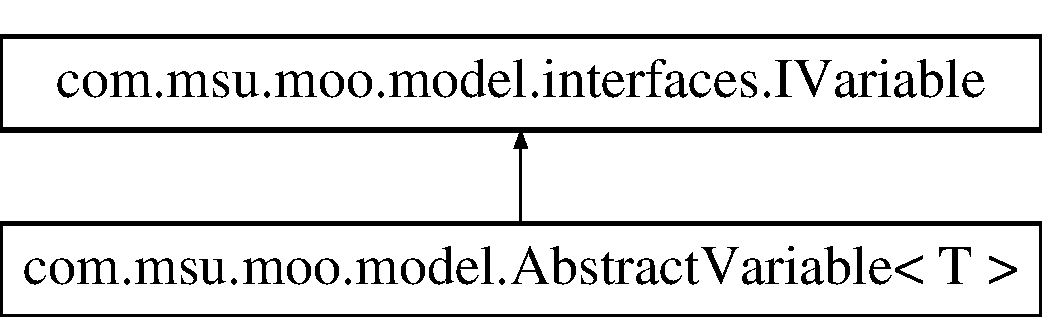
\includegraphics[height=2.000000cm]{classcom_1_1msu_1_1moo_1_1model_1_1AbstractVariable_3_01T_01_4}
\end{center}
\end{figure}
\subsection*{Public Member Functions}
\begin{DoxyCompactItemize}
\item 
abstract \hyperlink{interfacecom_1_1msu_1_1moo_1_1model_1_1interfaces_1_1IVariable}{I\-Variable} \hyperlink{classcom_1_1msu_1_1moo_1_1model_1_1AbstractVariable_3_01T_01_4_ab11df1a0613f42b0f1aed2226c666da2}{copy} ()
\item 
\hypertarget{classcom_1_1msu_1_1moo_1_1model_1_1AbstractVariable_3_01T_01_4_a12d90648f8d83ad81de5f807140fcf62}{{\bfseries Abstract\-Variable} (T \hyperlink{classcom_1_1msu_1_1moo_1_1model_1_1AbstractVariable_3_01T_01_4_ad584ca2577d331fbf04449fdcf2b6ed9}{obj})}\label{classcom_1_1msu_1_1moo_1_1model_1_1AbstractVariable_3_01T_01_4_a12d90648f8d83ad81de5f807140fcf62}

\item 
T \hyperlink{classcom_1_1msu_1_1moo_1_1model_1_1AbstractVariable_3_01T_01_4_a4c969f78e29f71436eb1f2db62fd43c5}{get} ()
\item 
void \hyperlink{classcom_1_1msu_1_1moo_1_1model_1_1AbstractVariable_3_01T_01_4_ad3b3dfcb1027411ca8adc0a2e82a42d2}{set} (Object \hyperlink{classcom_1_1msu_1_1moo_1_1model_1_1AbstractVariable_3_01T_01_4_ad584ca2577d331fbf04449fdcf2b6ed9}{obj})
\item 
\hypertarget{classcom_1_1msu_1_1moo_1_1model_1_1AbstractVariable_3_01T_01_4_a541a74317afb7a5296df1be518ca007b}{String {\bfseries to\-String} ()}\label{classcom_1_1msu_1_1moo_1_1model_1_1AbstractVariable_3_01T_01_4_a541a74317afb7a5296df1be518ca007b}

\end{DoxyCompactItemize}
\subsection*{Protected Attributes}
\begin{DoxyCompactItemize}
\item 
\hypertarget{classcom_1_1msu_1_1moo_1_1model_1_1AbstractVariable_3_01T_01_4_ad584ca2577d331fbf04449fdcf2b6ed9}{T \hyperlink{classcom_1_1msu_1_1moo_1_1model_1_1AbstractVariable_3_01T_01_4_ad584ca2577d331fbf04449fdcf2b6ed9}{obj}}\label{classcom_1_1msu_1_1moo_1_1model_1_1AbstractVariable_3_01T_01_4_ad584ca2577d331fbf04449fdcf2b6ed9}

\begin{DoxyCompactList}\small\item\em list that contains all the values \end{DoxyCompactList}\end{DoxyCompactItemize}


\subsection{Member Function Documentation}
\hypertarget{classcom_1_1msu_1_1moo_1_1model_1_1AbstractVariable_3_01T_01_4_ab11df1a0613f42b0f1aed2226c666da2}{\index{com\-::msu\-::moo\-::model\-::\-Abstract\-Variable$<$ T $>$@{com\-::msu\-::moo\-::model\-::\-Abstract\-Variable$<$ T $>$}!copy@{copy}}
\index{copy@{copy}!com::msu::moo::model::AbstractVariable< T >@{com\-::msu\-::moo\-::model\-::\-Abstract\-Variable$<$ T $>$}}
\subsubsection[{copy}]{\setlength{\rightskip}{0pt plus 5cm}abstract {\bf I\-Variable} com.\-msu.\-moo.\-model.\-Abstract\-Variable$<$ T $>$.copy (
\begin{DoxyParamCaption}
{}
\end{DoxyParamCaption}
)\hspace{0.3cm}{\ttfamily [abstract]}}}\label{classcom_1_1msu_1_1moo_1_1model_1_1AbstractVariable_3_01T_01_4_ab11df1a0613f42b0f1aed2226c666da2}
\begin{DoxyReturn}{Returns}
copy of the current variable 
\end{DoxyReturn}


Implements \hyperlink{interfacecom_1_1msu_1_1moo_1_1model_1_1interfaces_1_1IVariable_aca748275c7293a63283ada1a665c6c28}{com.\-msu.\-moo.\-model.\-interfaces.\-I\-Variable}.

\hypertarget{classcom_1_1msu_1_1moo_1_1model_1_1AbstractVariable_3_01T_01_4_a4c969f78e29f71436eb1f2db62fd43c5}{\index{com\-::msu\-::moo\-::model\-::\-Abstract\-Variable$<$ T $>$@{com\-::msu\-::moo\-::model\-::\-Abstract\-Variable$<$ T $>$}!get@{get}}
\index{get@{get}!com::msu::moo::model::AbstractVariable< T >@{com\-::msu\-::moo\-::model\-::\-Abstract\-Variable$<$ T $>$}}
\subsubsection[{get}]{\setlength{\rightskip}{0pt plus 5cm}T com.\-msu.\-moo.\-model.\-Abstract\-Variable$<$ T $>$.get (
\begin{DoxyParamCaption}
{}
\end{DoxyParamCaption}
)\hspace{0.3cm}{\ttfamily [inline]}}}\label{classcom_1_1msu_1_1moo_1_1model_1_1AbstractVariable_3_01T_01_4_a4c969f78e29f71436eb1f2db62fd43c5}
\begin{DoxyReturn}{Returns}
the variable by it self 
\end{DoxyReturn}


Implements \hyperlink{interfacecom_1_1msu_1_1moo_1_1model_1_1interfaces_1_1IVariable_a5d91fb013a9135144d975aa05b5f1b29}{com.\-msu.\-moo.\-model.\-interfaces.\-I\-Variable}.

\hypertarget{classcom_1_1msu_1_1moo_1_1model_1_1AbstractVariable_3_01T_01_4_ad3b3dfcb1027411ca8adc0a2e82a42d2}{\index{com\-::msu\-::moo\-::model\-::\-Abstract\-Variable$<$ T $>$@{com\-::msu\-::moo\-::model\-::\-Abstract\-Variable$<$ T $>$}!set@{set}}
\index{set@{set}!com::msu::moo::model::AbstractVariable< T >@{com\-::msu\-::moo\-::model\-::\-Abstract\-Variable$<$ T $>$}}
\subsubsection[{set}]{\setlength{\rightskip}{0pt plus 5cm}void com.\-msu.\-moo.\-model.\-Abstract\-Variable$<$ T $>$.set (
\begin{DoxyParamCaption}
\item[{Object}]{obj}
\end{DoxyParamCaption}
)\hspace{0.3cm}{\ttfamily [inline]}}}\label{classcom_1_1msu_1_1moo_1_1model_1_1AbstractVariable_3_01T_01_4_ad3b3dfcb1027411ca8adc0a2e82a42d2}
Set the value for the variable 

Implements \hyperlink{interfacecom_1_1msu_1_1moo_1_1model_1_1interfaces_1_1IVariable_a3bc30a747b2ee3c161fa3f6af8a9a061}{com.\-msu.\-moo.\-model.\-interfaces.\-I\-Variable}.



The documentation for this class was generated from the following file\-:\begin{DoxyCompactItemize}
\item 
src/main/java/com/msu/moo/model/Abstract\-Variable.\-java\end{DoxyCompactItemize}

\hypertarget{classcom_1_1msu_1_1moo_1_1util_1_1BashExecutor}{\section{com.\-msu.\-moo.\-util.\-Bash\-Executor Class Reference}
\label{classcom_1_1msu_1_1moo_1_1util_1_1BashExecutor}\index{com.\-msu.\-moo.\-util.\-Bash\-Executor@{com.\-msu.\-moo.\-util.\-Bash\-Executor}}
}
\subsection*{Static Public Member Functions}
\begin{DoxyCompactItemize}
\item 
\hypertarget{classcom_1_1msu_1_1moo_1_1util_1_1BashExecutor_ae22f572f361bf166ac37bd59d239799e}{static String {\bfseries execute} (String command)}\label{classcom_1_1msu_1_1moo_1_1util_1_1BashExecutor_ae22f572f361bf166ac37bd59d239799e}

\item 
\hypertarget{classcom_1_1msu_1_1moo_1_1util_1_1BashExecutor_a80c3b04f25b6c06b8f68a9e6dbc018bc}{static String {\bfseries from\-Stream} (Input\-Stream is)}\label{classcom_1_1msu_1_1moo_1_1util_1_1BashExecutor_a80c3b04f25b6c06b8f68a9e6dbc018bc}

\end{DoxyCompactItemize}


The documentation for this class was generated from the following file\-:\begin{DoxyCompactItemize}
\item 
src/main/java/com/msu/moo/util/Bash\-Executor.\-java\end{DoxyCompactItemize}

\hypertarget{classcom_1_1msu_1_1moo_1_1operators_1_1selection_1_1BinaryTournamentSelection}{\section{com.\-msu.\-moo.\-operators.\-selection.\-Binary\-Tournament\-Selection Class Reference}
\label{classcom_1_1msu_1_1moo_1_1operators_1_1selection_1_1BinaryTournamentSelection}\index{com.\-msu.\-moo.\-operators.\-selection.\-Binary\-Tournament\-Selection@{com.\-msu.\-moo.\-operators.\-selection.\-Binary\-Tournament\-Selection}}
}
Inheritance diagram for com.\-msu.\-moo.\-operators.\-selection.\-Binary\-Tournament\-Selection\-:\begin{figure}[H]
\begin{center}
\leavevmode
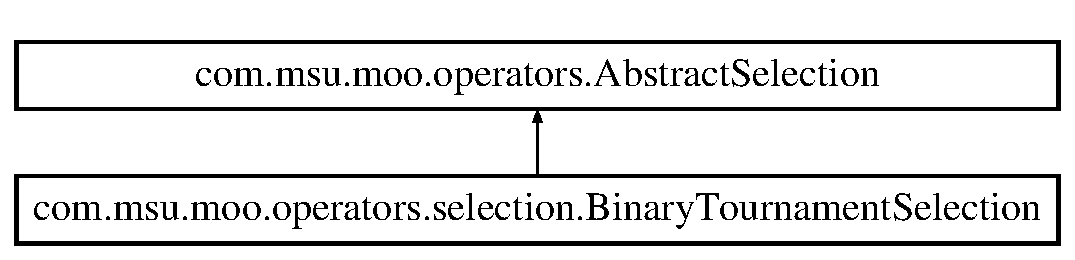
\includegraphics[height=2.000000cm]{classcom_1_1msu_1_1moo_1_1operators_1_1selection_1_1BinaryTournamentSelection}
\end{center}
\end{figure}
\subsection*{Public Member Functions}
\begin{DoxyCompactItemize}
\item 
\hyperlink{classcom_1_1msu_1_1moo_1_1operators_1_1selection_1_1BinaryTournamentSelection_a278003df852eb1ec89e0b41d313fcd01}{Binary\-Tournament\-Selection} (\hyperlink{classcom_1_1msu_1_1moo_1_1model_1_1solution_1_1SolutionSet}{Solution\-Set} \hyperlink{classcom_1_1msu_1_1moo_1_1operators_1_1AbstractSelection_ade84bd57f9d26c9d9b2e90bb6591b79c}{set}, Comparator$<$ \hyperlink{classcom_1_1msu_1_1moo_1_1model_1_1solution_1_1Solution}{Solution} $>$ \hyperlink{classcom_1_1msu_1_1moo_1_1operators_1_1selection_1_1BinaryTournamentSelection_ad167c5ef80c4ad0a0f1741bea8be5117}{cmp})
\item 
\hyperlink{classcom_1_1msu_1_1moo_1_1model_1_1solution_1_1Solution}{Solution} \hyperlink{classcom_1_1msu_1_1moo_1_1operators_1_1selection_1_1BinaryTournamentSelection_a061f5f41208fcecb04a559e7ed6e32d7}{next} ()
\end{DoxyCompactItemize}
\subsection*{Protected Member Functions}
\begin{DoxyCompactItemize}
\item 
\hypertarget{classcom_1_1msu_1_1moo_1_1operators_1_1selection_1_1BinaryTournamentSelection_a05157f4022e4c1785b25f8028a7e3e79}{void {\bfseries rnd\-Pool} ()}\label{classcom_1_1msu_1_1moo_1_1operators_1_1selection_1_1BinaryTournamentSelection_a05157f4022e4c1785b25f8028a7e3e79}

\end{DoxyCompactItemize}
\subsection*{Protected Attributes}
\begin{DoxyCompactItemize}
\item 
\hypertarget{classcom_1_1msu_1_1moo_1_1operators_1_1selection_1_1BinaryTournamentSelection_ad167c5ef80c4ad0a0f1741bea8be5117}{Comparator$<$ \hyperlink{classcom_1_1msu_1_1moo_1_1model_1_1solution_1_1Solution}{Solution} $>$ \hyperlink{classcom_1_1msu_1_1moo_1_1operators_1_1selection_1_1BinaryTournamentSelection_ad167c5ef80c4ad0a0f1741bea8be5117}{cmp}}\label{classcom_1_1msu_1_1moo_1_1operators_1_1selection_1_1BinaryTournamentSelection_ad167c5ef80c4ad0a0f1741bea8be5117}

\begin{DoxyCompactList}\small\item\em Comparator for choosing which solution is better. \end{DoxyCompactList}\item 
\hypertarget{classcom_1_1msu_1_1moo_1_1operators_1_1selection_1_1BinaryTournamentSelection_a1df311edb47efc73fc8401436c821168}{Queue$<$ \hyperlink{classcom_1_1msu_1_1moo_1_1model_1_1solution_1_1Solution}{Solution} $>$ \hyperlink{classcom_1_1msu_1_1moo_1_1operators_1_1selection_1_1BinaryTournamentSelection_a1df311edb47efc73fc8401436c821168}{q} = null}\label{classcom_1_1msu_1_1moo_1_1operators_1_1selection_1_1BinaryTournamentSelection_a1df311edb47efc73fc8401436c821168}

\begin{DoxyCompactList}\small\item\em current pool which is used for the selection \end{DoxyCompactList}\end{DoxyCompactItemize}


\subsection{Detailed Description}
This is a binary tournament select which could be used for sending always to individuals to a tournament and choose the winner by using a comparator! 

\subsection{Constructor \& Destructor Documentation}
\hypertarget{classcom_1_1msu_1_1moo_1_1operators_1_1selection_1_1BinaryTournamentSelection_a278003df852eb1ec89e0b41d313fcd01}{\index{com\-::msu\-::moo\-::operators\-::selection\-::\-Binary\-Tournament\-Selection@{com\-::msu\-::moo\-::operators\-::selection\-::\-Binary\-Tournament\-Selection}!Binary\-Tournament\-Selection@{Binary\-Tournament\-Selection}}
\index{Binary\-Tournament\-Selection@{Binary\-Tournament\-Selection}!com::msu::moo::operators::selection::BinaryTournamentSelection@{com\-::msu\-::moo\-::operators\-::selection\-::\-Binary\-Tournament\-Selection}}
\subsubsection[{Binary\-Tournament\-Selection}]{\setlength{\rightskip}{0pt plus 5cm}com.\-msu.\-moo.\-operators.\-selection.\-Binary\-Tournament\-Selection.\-Binary\-Tournament\-Selection (
\begin{DoxyParamCaption}
\item[{{\bf Solution\-Set}}]{set, }
\item[{Comparator$<$ {\bf Solution} $>$}]{cmp}
\end{DoxyParamCaption}
)\hspace{0.3cm}{\ttfamily [inline]}}}\label{classcom_1_1msu_1_1moo_1_1operators_1_1selection_1_1BinaryTournamentSelection_a278003df852eb1ec89e0b41d313fcd01}
Construct a binary tournament selector 
\begin{DoxyParams}{Parameters}
{\em set} & which should be used for selection \\
\hline
{\em cmp} & comparator which defines the winner of the tournament \\
\hline
\end{DoxyParams}


\subsection{Member Function Documentation}
\hypertarget{classcom_1_1msu_1_1moo_1_1operators_1_1selection_1_1BinaryTournamentSelection_a061f5f41208fcecb04a559e7ed6e32d7}{\index{com\-::msu\-::moo\-::operators\-::selection\-::\-Binary\-Tournament\-Selection@{com\-::msu\-::moo\-::operators\-::selection\-::\-Binary\-Tournament\-Selection}!next@{next}}
\index{next@{next}!com::msu::moo::operators::selection::BinaryTournamentSelection@{com\-::msu\-::moo\-::operators\-::selection\-::\-Binary\-Tournament\-Selection}}
\subsubsection[{next}]{\setlength{\rightskip}{0pt plus 5cm}{\bf Solution} com.\-msu.\-moo.\-operators.\-selection.\-Binary\-Tournament\-Selection.\-next (
\begin{DoxyParamCaption}
{}
\end{DoxyParamCaption}
)\hspace{0.3cm}{\ttfamily [inline]}}}\label{classcom_1_1msu_1_1moo_1_1operators_1_1selection_1_1BinaryTournamentSelection_a061f5f41208fcecb04a559e7ed6e32d7}
Create a binary tournament, choose the winner. If the pool is empty there is created a new one! \begin{DoxyReturn}{Returns}
winner of the tournament 
\end{DoxyReturn}


The documentation for this class was generated from the following file\-:\begin{DoxyCompactItemize}
\item 
src/main/java/com/msu/moo/operators/selection/Binary\-Tournament\-Selection.\-java\end{DoxyCompactItemize}

\hypertarget{classcom_1_1msu_1_1moo_1_1operators_1_1mutation_1_1BitFlipMutation}{\section{com.\-msu.\-moo.\-operators.\-mutation.\-Bit\-Flip\-Mutation Class Reference}
\label{classcom_1_1msu_1_1moo_1_1operators_1_1mutation_1_1BitFlipMutation}\index{com.\-msu.\-moo.\-operators.\-mutation.\-Bit\-Flip\-Mutation@{com.\-msu.\-moo.\-operators.\-mutation.\-Bit\-Flip\-Mutation}}
}
Inheritance diagram for com.\-msu.\-moo.\-operators.\-mutation.\-Bit\-Flip\-Mutation\-:\begin{figure}[H]
\begin{center}
\leavevmode
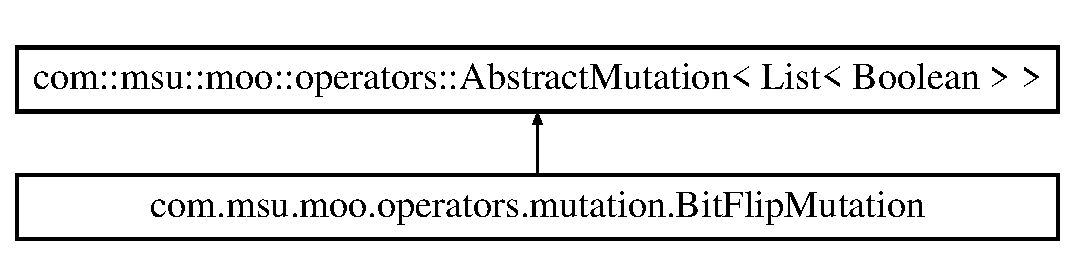
\includegraphics[height=2.000000cm]{classcom_1_1msu_1_1moo_1_1operators_1_1mutation_1_1BitFlipMutation}
\end{center}
\end{figure}
\subsection*{Public Member Functions}
\begin{DoxyCompactItemize}
\item 
\hyperlink{classcom_1_1msu_1_1moo_1_1operators_1_1mutation_1_1BitFlipMutation_a1acc2ca05bdc3e678e3614199ef5f619}{Bit\-Flip\-Mutation} ()
\item 
\hyperlink{classcom_1_1msu_1_1moo_1_1operators_1_1mutation_1_1BitFlipMutation_a15bc402d2403f5980fc7b246420175b8}{Bit\-Flip\-Mutation} (Double \hyperlink{classcom_1_1msu_1_1moo_1_1operators_1_1mutation_1_1BitFlipMutation_a171f6a7c34816318f48116e75eca4b7c}{probability})
\end{DoxyCompactItemize}
\subsection*{Protected Member Functions}
\begin{DoxyCompactItemize}
\item 
\hypertarget{classcom_1_1msu_1_1moo_1_1operators_1_1mutation_1_1BitFlipMutation_aa239884ac2562908ae65b5f129623e27}{void {\bfseries mutate\-\_\-} (List$<$ Boolean $>$ b)}\label{classcom_1_1msu_1_1moo_1_1operators_1_1mutation_1_1BitFlipMutation_aa239884ac2562908ae65b5f129623e27}

\end{DoxyCompactItemize}
\subsection*{Protected Attributes}
\begin{DoxyCompactItemize}
\item 
\hypertarget{classcom_1_1msu_1_1moo_1_1operators_1_1mutation_1_1BitFlipMutation_a171f6a7c34816318f48116e75eca4b7c}{Double \hyperlink{classcom_1_1msu_1_1moo_1_1operators_1_1mutation_1_1BitFlipMutation_a171f6a7c34816318f48116e75eca4b7c}{probability} = null}\label{classcom_1_1msu_1_1moo_1_1operators_1_1mutation_1_1BitFlipMutation_a171f6a7c34816318f48116e75eca4b7c}

\begin{DoxyCompactList}\small\item\em the probability that a bit is changed \end{DoxyCompactList}\end{DoxyCompactItemize}


\subsection{Detailed Description}
This is a basic \hyperlink{classcom_1_1msu_1_1moo_1_1operators_1_1mutation_1_1BitFlipMutation}{Bit\-Flip\-Mutation} which is allowed on all List$<$\-Boolean$>$ objects. There are two objects\-: there could be a fix probability or it is 1/length of object.

\mbox{[}0,0,1,0\mbox{]} -\/---$>$ \mbox{[}1,0,1,0\mbox{]} 

\subsection{Constructor \& Destructor Documentation}
\hypertarget{classcom_1_1msu_1_1moo_1_1operators_1_1mutation_1_1BitFlipMutation_a1acc2ca05bdc3e678e3614199ef5f619}{\index{com\-::msu\-::moo\-::operators\-::mutation\-::\-Bit\-Flip\-Mutation@{com\-::msu\-::moo\-::operators\-::mutation\-::\-Bit\-Flip\-Mutation}!Bit\-Flip\-Mutation@{Bit\-Flip\-Mutation}}
\index{Bit\-Flip\-Mutation@{Bit\-Flip\-Mutation}!com::msu::moo::operators::mutation::BitFlipMutation@{com\-::msu\-::moo\-::operators\-::mutation\-::\-Bit\-Flip\-Mutation}}
\subsubsection[{Bit\-Flip\-Mutation}]{\setlength{\rightskip}{0pt plus 5cm}com.\-msu.\-moo.\-operators.\-mutation.\-Bit\-Flip\-Mutation.\-Bit\-Flip\-Mutation (
\begin{DoxyParamCaption}
{}
\end{DoxyParamCaption}
)\hspace{0.3cm}{\ttfamily [inline]}}}\label{classcom_1_1msu_1_1moo_1_1operators_1_1mutation_1_1BitFlipMutation_a1acc2ca05bdc3e678e3614199ef5f619}
Normal constructor with dynamic probability \hypertarget{classcom_1_1msu_1_1moo_1_1operators_1_1mutation_1_1BitFlipMutation_a15bc402d2403f5980fc7b246420175b8}{\index{com\-::msu\-::moo\-::operators\-::mutation\-::\-Bit\-Flip\-Mutation@{com\-::msu\-::moo\-::operators\-::mutation\-::\-Bit\-Flip\-Mutation}!Bit\-Flip\-Mutation@{Bit\-Flip\-Mutation}}
\index{Bit\-Flip\-Mutation@{Bit\-Flip\-Mutation}!com::msu::moo::operators::mutation::BitFlipMutation@{com\-::msu\-::moo\-::operators\-::mutation\-::\-Bit\-Flip\-Mutation}}
\subsubsection[{Bit\-Flip\-Mutation}]{\setlength{\rightskip}{0pt plus 5cm}com.\-msu.\-moo.\-operators.\-mutation.\-Bit\-Flip\-Mutation.\-Bit\-Flip\-Mutation (
\begin{DoxyParamCaption}
\item[{Double}]{probability}
\end{DoxyParamCaption}
)\hspace{0.3cm}{\ttfamily [inline]}}}\label{classcom_1_1msu_1_1moo_1_1operators_1_1mutation_1_1BitFlipMutation_a15bc402d2403f5980fc7b246420175b8}
Constructor which fixes the probability for all inputs. 
\begin{DoxyParams}{Parameters}
{\em probability} & that a bit is changed \\
\hline
\end{DoxyParams}


The documentation for this class was generated from the following file\-:\begin{DoxyCompactItemize}
\item 
src/main/java/com/msu/moo/operators/mutation/Bit\-Flip\-Mutation.\-java\end{DoxyCompactItemize}

\hypertarget{classcom_1_1msu_1_1moo_1_1visualization_1_1BoxPlot}{\section{com.\-msu.\-moo.\-visualization.\-Box\-Plot Class Reference}
\label{classcom_1_1msu_1_1moo_1_1visualization_1_1BoxPlot}\index{com.\-msu.\-moo.\-visualization.\-Box\-Plot@{com.\-msu.\-moo.\-visualization.\-Box\-Plot}}
}
Inheritance diagram for com.\-msu.\-moo.\-visualization.\-Box\-Plot\-:\begin{figure}[H]
\begin{center}
\leavevmode
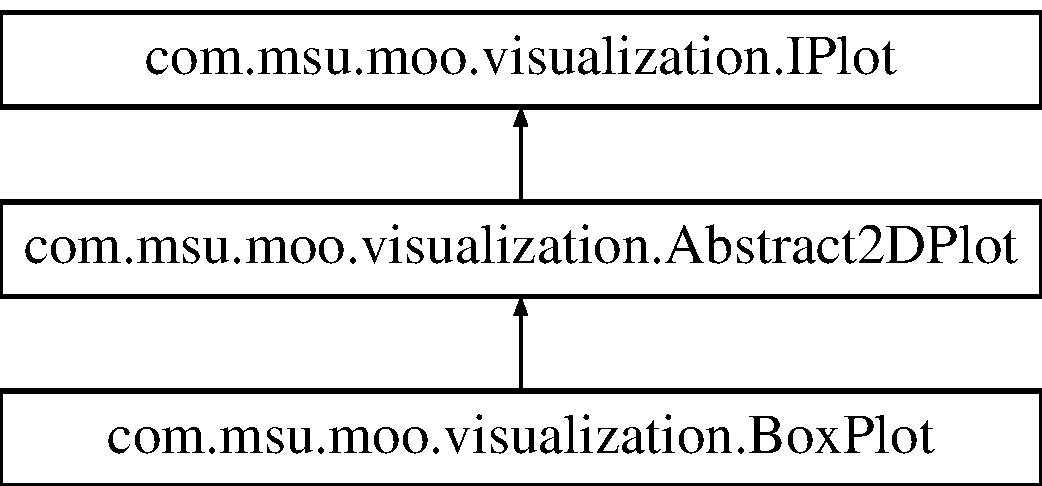
\includegraphics[height=3.000000cm]{classcom_1_1msu_1_1moo_1_1visualization_1_1BoxPlot}
\end{center}
\end{figure}
\subsection*{Public Member Functions}
\begin{DoxyCompactItemize}
\item 
\hypertarget{classcom_1_1msu_1_1moo_1_1visualization_1_1BoxPlot_a55aa11ce9cc53f6eb15c2aa652d104a5}{{\bfseries Box\-Plot} (String title)}\label{classcom_1_1msu_1_1moo_1_1visualization_1_1BoxPlot_a55aa11ce9cc53f6eb15c2aa652d104a5}

\item 
\hypertarget{classcom_1_1msu_1_1moo_1_1visualization_1_1BoxPlot_ab03b603543005ad2490338eed1f36401}{void {\bfseries add} (List$<$ Double $>$ l, String name)}\label{classcom_1_1msu_1_1moo_1_1visualization_1_1BoxPlot_ab03b603543005ad2490338eed1f36401}

\item 
J\-Free\-Chart \hyperlink{classcom_1_1msu_1_1moo_1_1visualization_1_1BoxPlot_acfbffc8df459e92c6b39108371fd462c}{get\-Chart} ()
\end{DoxyCompactItemize}
\subsection*{Protected Attributes}
\begin{DoxyCompactItemize}
\item 
\hypertarget{classcom_1_1msu_1_1moo_1_1visualization_1_1BoxPlot_a73e78f7007cbce86e9b45ced47b2797b}{Default\-Box\-And\-Whisker\-Category\-Dataset {\bfseries set} = new Default\-Box\-And\-Whisker\-Category\-Dataset()}\label{classcom_1_1msu_1_1moo_1_1visualization_1_1BoxPlot_a73e78f7007cbce86e9b45ced47b2797b}

\end{DoxyCompactItemize}


\subsection{Member Function Documentation}
\hypertarget{classcom_1_1msu_1_1moo_1_1visualization_1_1BoxPlot_acfbffc8df459e92c6b39108371fd462c}{\index{com\-::msu\-::moo\-::visualization\-::\-Box\-Plot@{com\-::msu\-::moo\-::visualization\-::\-Box\-Plot}!get\-Chart@{get\-Chart}}
\index{get\-Chart@{get\-Chart}!com::msu::moo::visualization::BoxPlot@{com\-::msu\-::moo\-::visualization\-::\-Box\-Plot}}
\subsubsection[{get\-Chart}]{\setlength{\rightskip}{0pt plus 5cm}J\-Free\-Chart com.\-msu.\-moo.\-visualization.\-Box\-Plot.\-get\-Chart (
\begin{DoxyParamCaption}
{}
\end{DoxyParamCaption}
)\hspace{0.3cm}{\ttfamily [inline]}}}\label{classcom_1_1msu_1_1moo_1_1visualization_1_1BoxPlot_acfbffc8df459e92c6b39108371fd462c}
Every Plot needs the chart frame to visualize the results \begin{DoxyReturn}{Returns}
chart frame to make it visible 
\end{DoxyReturn}


Implements \hyperlink{interfacecom_1_1msu_1_1moo_1_1visualization_1_1IPlot_ae45c2987d112fbf5bc5af7864fb50ecd}{com.\-msu.\-moo.\-visualization.\-I\-Plot}.



The documentation for this class was generated from the following file\-:\begin{DoxyCompactItemize}
\item 
src/main/java/com/msu/moo/visualization/Box\-Plot.\-java\end{DoxyCompactItemize}

\hypertarget{classcom_1_1msu_1_1moo_1_1Configuration}{\section{com.\-msu.\-moo.\-Configuration Class Reference}
\label{classcom_1_1msu_1_1moo_1_1Configuration}\index{com.\-msu.\-moo.\-Configuration@{com.\-msu.\-moo.\-Configuration}}
}
\subsection*{Static Public Attributes}
\begin{DoxyCompactItemize}
\item 
\hypertarget{classcom_1_1msu_1_1moo_1_1Configuration_a2750209761c81fda824cafb4ad0bf198}{static String \hyperlink{classcom_1_1msu_1_1moo_1_1Configuration_a2750209761c81fda824cafb4ad0bf198}{path\-To\-E\-A\-F} = \char`\"{}vendor/aft-\/0.\-95/eaf\char`\"{}}\label{classcom_1_1msu_1_1moo_1_1Configuration_a2750209761c81fda824cafb4ad0bf198}

\begin{DoxyCompactList}\small\item\em path to Fonseca's E\-A\-F C Implementation \end{DoxyCompactList}\item 
\hypertarget{classcom_1_1msu_1_1moo_1_1Configuration_a312152f3e35cc90f11345a3be3b64231}{static String \hyperlink{classcom_1_1msu_1_1moo_1_1Configuration_a312152f3e35cc90f11345a3be3b64231}{path\-To\-H\-V} = \char`\"{}vendor/hv-\/1.\-3-\/src/hv\char`\"{}}\label{classcom_1_1msu_1_1moo_1_1Configuration_a312152f3e35cc90f11345a3be3b64231}

\begin{DoxyCompactList}\small\item\em path to Fonseca's Hypervolume C Implementation \end{DoxyCompactList}\end{DoxyCompactItemize}


The documentation for this class was generated from the following file\-:\begin{DoxyCompactItemize}
\item 
src/main/java/com/msu/moo/Configuration.\-java\end{DoxyCompactItemize}

\hypertarget{classcom_1_1msu_1_1moo_1_1operators_1_1crossover_1_1CrossoverUtil}{\section{com.\-msu.\-moo.\-operators.\-crossover.\-Crossover\-Util Class Reference}
\label{classcom_1_1msu_1_1moo_1_1operators_1_1crossover_1_1CrossoverUtil}\index{com.\-msu.\-moo.\-operators.\-crossover.\-Crossover\-Util@{com.\-msu.\-moo.\-operators.\-crossover.\-Crossover\-Util}}
}
\subsection*{Static Public Member Functions}
\begin{DoxyCompactItemize}
\item 
static Pair$<$ Integer, Integer $>$ \hyperlink{classcom_1_1msu_1_1moo_1_1operators_1_1crossover_1_1CrossoverUtil_a3f5d27607b9ebc9d5a860d326cacba75}{get\-Section} (int length)
\end{DoxyCompactItemize}


\subsection{Member Function Documentation}
\hypertarget{classcom_1_1msu_1_1moo_1_1operators_1_1crossover_1_1CrossoverUtil_a3f5d27607b9ebc9d5a860d326cacba75}{\index{com\-::msu\-::moo\-::operators\-::crossover\-::\-Crossover\-Util@{com\-::msu\-::moo\-::operators\-::crossover\-::\-Crossover\-Util}!get\-Section@{get\-Section}}
\index{get\-Section@{get\-Section}!com::msu::moo::operators::crossover::CrossoverUtil@{com\-::msu\-::moo\-::operators\-::crossover\-::\-Crossover\-Util}}
\subsubsection[{get\-Section}]{\setlength{\rightskip}{0pt plus 5cm}static Pair$<$Integer, Integer$>$ com.\-msu.\-moo.\-operators.\-crossover.\-Crossover\-Util.\-get\-Section (
\begin{DoxyParamCaption}
\item[{int}]{length}
\end{DoxyParamCaption}
)\hspace{0.3cm}{\ttfamily [inline]}, {\ttfamily [static]}}}\label{classcom_1_1msu_1_1moo_1_1operators_1_1crossover_1_1CrossoverUtil_a3f5d27607b9ebc9d5a860d326cacba75}
Return always a section from a allele, which means a lower and a upper bound. 
\begin{DoxyParams}{Parameters}
{\em length} & maximal length \\
\hline
\end{DoxyParams}
\begin{DoxyReturn}{Returns}
pair of integer. lb and ub. 
\end{DoxyReturn}


The documentation for this class was generated from the following file\-:\begin{DoxyCompactItemize}
\item 
src/main/java/com/msu/moo/operators/crossover/Crossover\-Util.\-java\end{DoxyCompactItemize}

\hypertarget{classcom_1_1msu_1_1moo_1_1util_1_1indicator_1_1CrowdingIndicator}{\section{com.\-msu.\-moo.\-util.\-indicator.\-Crowding\-Indicator Class Reference}
\label{classcom_1_1msu_1_1moo_1_1util_1_1indicator_1_1CrowdingIndicator}\index{com.\-msu.\-moo.\-util.\-indicator.\-Crowding\-Indicator@{com.\-msu.\-moo.\-util.\-indicator.\-Crowding\-Indicator}}
}
Inheritance diagram for com.\-msu.\-moo.\-util.\-indicator.\-Crowding\-Indicator\-:\begin{figure}[H]
\begin{center}
\leavevmode
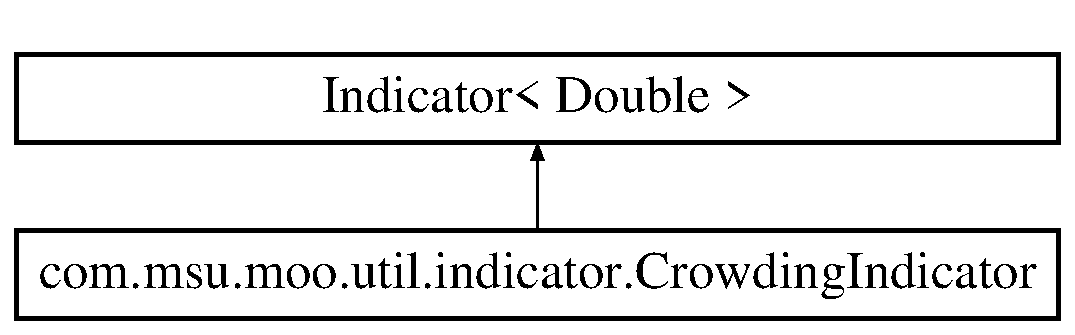
\includegraphics[height=2.000000cm]{classcom_1_1msu_1_1moo_1_1util_1_1indicator_1_1CrowdingIndicator}
\end{center}
\end{figure}
\subsection*{Public Member Functions}
\begin{DoxyCompactItemize}
\item 
\hypertarget{classcom_1_1msu_1_1moo_1_1util_1_1indicator_1_1CrowdingIndicator_a2a08f9285b560a4fd2213022672d100a}{void {\bfseries calculate} (Map$<$ \hyperlink{classcom_1_1msu_1_1moo_1_1model_1_1solution_1_1Solution}{Solution}, Double $>$ map, \hyperlink{classcom_1_1msu_1_1moo_1_1model_1_1solution_1_1SolutionSet}{Solution\-Set} solutions)}\label{classcom_1_1msu_1_1moo_1_1util_1_1indicator_1_1CrowdingIndicator_a2a08f9285b560a4fd2213022672d100a}

\end{DoxyCompactItemize}


The documentation for this class was generated from the following file\-:\begin{DoxyCompactItemize}
\item 
src/main/java/com/msu/moo/util/indicator/Crowding\-Indicator.\-java\end{DoxyCompactItemize}

\hypertarget{classcom_1_1msu_1_1moo_1_1operators_1_1crossover_1_1permutation_1_1CycleCrossover_3_01T_01_4}{\section{com.\-msu.\-moo.\-operators.\-crossover.\-permutation.\-Cycle\-Crossover$<$ T $>$ Class Reference}
\label{classcom_1_1msu_1_1moo_1_1operators_1_1crossover_1_1permutation_1_1CycleCrossover_3_01T_01_4}\index{com.\-msu.\-moo.\-operators.\-crossover.\-permutation.\-Cycle\-Crossover$<$ T $>$@{com.\-msu.\-moo.\-operators.\-crossover.\-permutation.\-Cycle\-Crossover$<$ T $>$}}
}
Inheritance diagram for com.\-msu.\-moo.\-operators.\-crossover.\-permutation.\-Cycle\-Crossover$<$ T $>$\-:\begin{figure}[H]
\begin{center}
\leavevmode
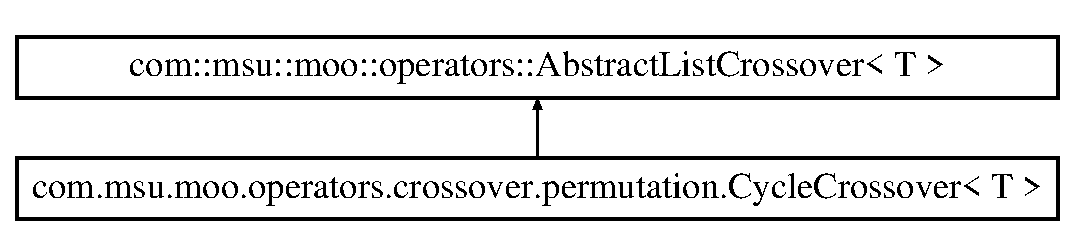
\includegraphics[height=2.000000cm]{classcom_1_1msu_1_1moo_1_1operators_1_1crossover_1_1permutation_1_1CycleCrossover_3_01T_01_4}
\end{center}
\end{figure}
\subsection*{Protected Member Functions}
\begin{DoxyCompactItemize}
\item 
\hypertarget{classcom_1_1msu_1_1moo_1_1operators_1_1crossover_1_1permutation_1_1CycleCrossover_3_01T_01_4_aac01361127e47317afa35f8b4e88e5f2}{List$<$ List$<$ T $>$ $>$ {\bfseries crossover\-Lists} (List$<$ T $>$ a, List$<$ T $>$ b)}\label{classcom_1_1msu_1_1moo_1_1operators_1_1crossover_1_1permutation_1_1CycleCrossover_3_01T_01_4_aac01361127e47317afa35f8b4e88e5f2}

\item 
\hypertarget{classcom_1_1msu_1_1moo_1_1operators_1_1crossover_1_1permutation_1_1CycleCrossover_3_01T_01_4_aad24f0f50a05a39157165d045f97dc41}{List$<$ List$<$ T $>$ $>$ {\bfseries crossover\-\_\-} (List$<$ T $>$ a, List$<$ T $>$ b, int idx)}\label{classcom_1_1msu_1_1moo_1_1operators_1_1crossover_1_1permutation_1_1CycleCrossover_3_01T_01_4_aad24f0f50a05a39157165d045f97dc41}

\end{DoxyCompactItemize}


\subsection{Detailed Description}
This is the single point crossover where a list with any type could but cut in a half and recombined with another half.

\mbox{[}0,1,2,3,4\mbox{]} and \mbox{[}4,3,2,1,0\mbox{]} and point is one leads to

\mbox{[}0\mbox{]} + \mbox{[}3,2,1,0\mbox{]} = \mbox{[}0,3,2,1,0\mbox{]} and \mbox{[}4\mbox{]} + \mbox{[}1,2,3,4\mbox{]} = \mbox{[}4,1,2,3,4\mbox{]} 

The documentation for this class was generated from the following file\-:\begin{DoxyCompactItemize}
\item 
src/main/java/com/msu/moo/operators/crossover/permutation/Cycle\-Crossover.\-java\end{DoxyCompactItemize}

\hypertarget{classcom_1_1msu_1_1moo_1_1model_1_1variables_1_1DoubleListVariable}{\section{com.\-msu.\-moo.\-model.\-variables.\-Double\-List\-Variable Class Reference}
\label{classcom_1_1msu_1_1moo_1_1model_1_1variables_1_1DoubleListVariable}\index{com.\-msu.\-moo.\-model.\-variables.\-Double\-List\-Variable@{com.\-msu.\-moo.\-model.\-variables.\-Double\-List\-Variable}}
}
Inheritance diagram for com.\-msu.\-moo.\-model.\-variables.\-Double\-List\-Variable\-:\begin{figure}[H]
\begin{center}
\leavevmode
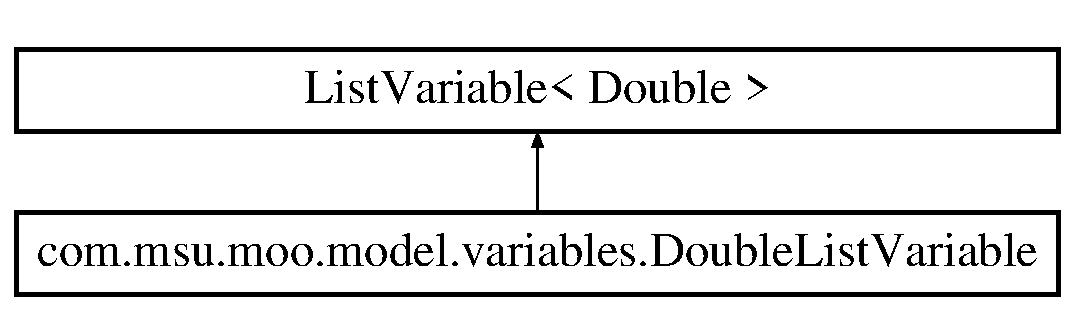
\includegraphics[height=2.000000cm]{classcom_1_1msu_1_1moo_1_1model_1_1variables_1_1DoubleListVariable}
\end{center}
\end{figure}
\subsection*{Public Member Functions}
\begin{DoxyCompactItemize}
\item 
\hypertarget{classcom_1_1msu_1_1moo_1_1model_1_1variables_1_1DoubleListVariable_a89e8cdbe9a215ffa3946a2ededbf01ab}{{\bfseries Double\-List\-Variable} (List$<$ Double $>$ list)}\label{classcom_1_1msu_1_1moo_1_1model_1_1variables_1_1DoubleListVariable_a89e8cdbe9a215ffa3946a2ededbf01ab}

\item 
\hypertarget{classcom_1_1msu_1_1moo_1_1model_1_1variables_1_1DoubleListVariable_adee645c8b18616dffccbb9ce0f34ce84}{\hyperlink{interfacecom_1_1msu_1_1moo_1_1model_1_1interfaces_1_1IVariable}{I\-Variable} {\bfseries copy} ()}\label{classcom_1_1msu_1_1moo_1_1model_1_1variables_1_1DoubleListVariable_adee645c8b18616dffccbb9ce0f34ce84}

\end{DoxyCompactItemize}


The documentation for this class was generated from the following file\-:\begin{DoxyCompactItemize}
\item 
src/main/java/com/msu/moo/model/variables/Double\-List\-Variable.\-java\end{DoxyCompactItemize}

\hypertarget{classcom_1_1msu_1_1moo_1_1model_1_1variables_1_1DoubleListVariableFactory_3_01P_01extends_01IProblem_01_4}{\section{com.\-msu.\-moo.\-model.\-variables.\-Double\-List\-Variable\-Factory$<$ P extends I\-Problem $>$ Class Reference}
\label{classcom_1_1msu_1_1moo_1_1model_1_1variables_1_1DoubleListVariableFactory_3_01P_01extends_01IProblem_01_4}\index{com.\-msu.\-moo.\-model.\-variables.\-Double\-List\-Variable\-Factory$<$ P extends I\-Problem $>$@{com.\-msu.\-moo.\-model.\-variables.\-Double\-List\-Variable\-Factory$<$ P extends I\-Problem $>$}}
}
Inheritance diagram for com.\-msu.\-moo.\-model.\-variables.\-Double\-List\-Variable\-Factory$<$ P extends I\-Problem $>$\-:\begin{figure}[H]
\begin{center}
\leavevmode
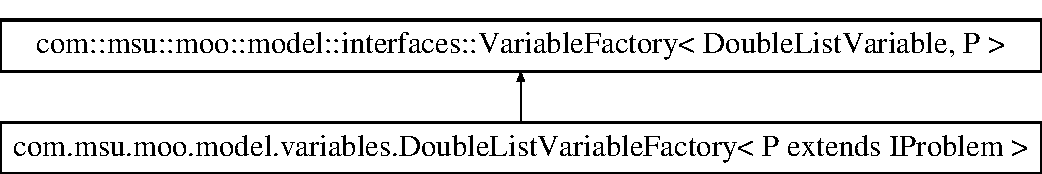
\includegraphics[height=2.000000cm]{classcom_1_1msu_1_1moo_1_1model_1_1variables_1_1DoubleListVariableFactory_3_01P_01extends_01IProblem_01_4}
\end{center}
\end{figure}
\subsection*{Public Member Functions}
\begin{DoxyCompactItemize}
\item 
\hypertarget{classcom_1_1msu_1_1moo_1_1model_1_1variables_1_1DoubleListVariableFactory_3_01P_01extends_01IProblem_01_4_a2ebfc6de5bb1dcb0ea17fc99e7ace5a2}{{\bfseries Double\-List\-Variable\-Factory} (int \hyperlink{classcom_1_1msu_1_1moo_1_1model_1_1variables_1_1DoubleListVariableFactory_3_01P_01extends_01IProblem_01_4_aebad65c096025aac60ce75e18ffedb89}{length})}\label{classcom_1_1msu_1_1moo_1_1model_1_1variables_1_1DoubleListVariableFactory_3_01P_01extends_01IProblem_01_4_a2ebfc6de5bb1dcb0ea17fc99e7ace5a2}

\item 
\hypertarget{classcom_1_1msu_1_1moo_1_1model_1_1variables_1_1DoubleListVariableFactory_3_01P_01extends_01IProblem_01_4_a2db71ce6af7784f9ce5973e0cba8e772}{{\bfseries Double\-List\-Variable\-Factory} (int \hyperlink{classcom_1_1msu_1_1moo_1_1model_1_1variables_1_1DoubleListVariableFactory_3_01P_01extends_01IProblem_01_4_aebad65c096025aac60ce75e18ffedb89}{length}, double\mbox{[}$\,$\mbox{]} \hyperlink{classcom_1_1msu_1_1moo_1_1model_1_1variables_1_1DoubleListVariableFactory_3_01P_01extends_01IProblem_01_4_ab60f1b1a92893ae3fa571b3374471a52}{range})}\label{classcom_1_1msu_1_1moo_1_1model_1_1variables_1_1DoubleListVariableFactory_3_01P_01extends_01IProblem_01_4_a2db71ce6af7784f9ce5973e0cba8e772}

\item 
\hypertarget{classcom_1_1msu_1_1moo_1_1model_1_1variables_1_1DoubleListVariableFactory_3_01P_01extends_01IProblem_01_4_a546ae37d9583af9efe111d00863009c9}{\hyperlink{classcom_1_1msu_1_1moo_1_1model_1_1variables_1_1DoubleListVariable}{Double\-List\-Variable} {\bfseries create} (P problem)}\label{classcom_1_1msu_1_1moo_1_1model_1_1variables_1_1DoubleListVariableFactory_3_01P_01extends_01IProblem_01_4_a546ae37d9583af9efe111d00863009c9}

\end{DoxyCompactItemize}
\subsection*{Protected Attributes}
\begin{DoxyCompactItemize}
\item 
\hypertarget{classcom_1_1msu_1_1moo_1_1model_1_1variables_1_1DoubleListVariableFactory_3_01P_01extends_01IProblem_01_4_aebad65c096025aac60ce75e18ffedb89}{int \hyperlink{classcom_1_1msu_1_1moo_1_1model_1_1variables_1_1DoubleListVariableFactory_3_01P_01extends_01IProblem_01_4_aebad65c096025aac60ce75e18ffedb89}{length}}\label{classcom_1_1msu_1_1moo_1_1model_1_1variables_1_1DoubleListVariableFactory_3_01P_01extends_01IProblem_01_4_aebad65c096025aac60ce75e18ffedb89}

\begin{DoxyCompactList}\small\item\em length of the vector \end{DoxyCompactList}\item 
\hypertarget{classcom_1_1msu_1_1moo_1_1model_1_1variables_1_1DoubleListVariableFactory_3_01P_01extends_01IProblem_01_4_ab60f1b1a92893ae3fa571b3374471a52}{double\mbox{[}$\,$\mbox{]} \hyperlink{classcom_1_1msu_1_1moo_1_1model_1_1variables_1_1DoubleListVariableFactory_3_01P_01extends_01IProblem_01_4_ab60f1b1a92893ae3fa571b3374471a52}{range} = new double\mbox{[}$\,$\mbox{]}\{ Double.\-M\-I\-N\-\_\-\-V\-A\-L\-U\-E, Double.\-M\-A\-X\-\_\-\-V\-A\-L\-U\-E\}}\label{classcom_1_1msu_1_1moo_1_1model_1_1variables_1_1DoubleListVariableFactory_3_01P_01extends_01IProblem_01_4_ab60f1b1a92893ae3fa571b3374471a52}

\begin{DoxyCompactList}\small\item\em length of the vector \end{DoxyCompactList}\end{DoxyCompactItemize}


The documentation for this class was generated from the following file\-:\begin{DoxyCompactItemize}
\item 
src/main/java/com/msu/moo/model/variables/Double\-List\-Variable\-Factory.\-java\end{DoxyCompactItemize}

\hypertarget{classcom_1_1msu_1_1moo_1_1operators_1_1crossover_1_1permutation_1_1EdgeRecombinationCrossover_3_01T_01_4}{\section{com.\-msu.\-moo.\-operators.\-crossover.\-permutation.\-Edge\-Recombination\-Crossover$<$ T $>$ Class Reference}
\label{classcom_1_1msu_1_1moo_1_1operators_1_1crossover_1_1permutation_1_1EdgeRecombinationCrossover_3_01T_01_4}\index{com.\-msu.\-moo.\-operators.\-crossover.\-permutation.\-Edge\-Recombination\-Crossover$<$ T $>$@{com.\-msu.\-moo.\-operators.\-crossover.\-permutation.\-Edge\-Recombination\-Crossover$<$ T $>$}}
}
Inheritance diagram for com.\-msu.\-moo.\-operators.\-crossover.\-permutation.\-Edge\-Recombination\-Crossover$<$ T $>$\-:\begin{figure}[H]
\begin{center}
\leavevmode
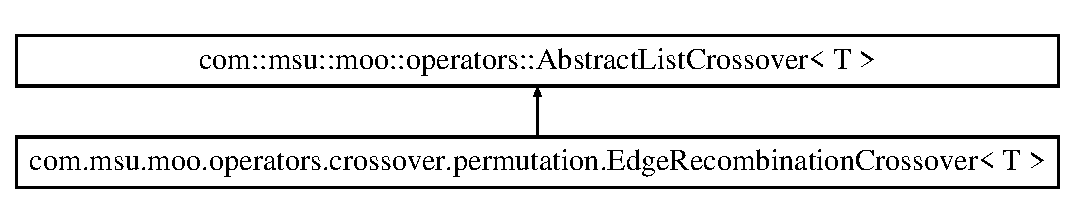
\includegraphics[height=2.000000cm]{classcom_1_1msu_1_1moo_1_1operators_1_1crossover_1_1permutation_1_1EdgeRecombinationCrossover_3_01T_01_4}
\end{center}
\end{figure}
\subsection*{Protected Member Functions}
\begin{DoxyCompactItemize}
\item 
\hypertarget{classcom_1_1msu_1_1moo_1_1operators_1_1crossover_1_1permutation_1_1EdgeRecombinationCrossover_3_01T_01_4_a99458e63b59009a585d6b4cf1799d80e}{List$<$ T $>$ {\bfseries crossover\-\_\-} (Map$<$ T, Hash\-Set$<$ T $>$$>$ map, List$<$ T $>$ l, int point)}\label{classcom_1_1msu_1_1moo_1_1operators_1_1crossover_1_1permutation_1_1EdgeRecombinationCrossover_3_01T_01_4_a99458e63b59009a585d6b4cf1799d80e}

\item 
\hypertarget{classcom_1_1msu_1_1moo_1_1operators_1_1crossover_1_1permutation_1_1EdgeRecombinationCrossover_3_01T_01_4_abd4e62911d49e28b2844cfbf01d673b9}{List$<$ List$<$ T $>$ $>$ {\bfseries crossover\-Lists} (List$<$ T $>$ a, List$<$ T $>$ b)}\label{classcom_1_1msu_1_1moo_1_1operators_1_1crossover_1_1permutation_1_1EdgeRecombinationCrossover_3_01T_01_4_abd4e62911d49e28b2844cfbf01d673b9}

\end{DoxyCompactItemize}


The documentation for this class was generated from the following file\-:\begin{DoxyCompactItemize}
\item 
src/main/java/com/msu/moo/operators/crossover/permutation/Edge\-Recombination\-Crossover.\-java\end{DoxyCompactItemize}

\hypertarget{classcom_1_1msu_1_1moo_1_1fonseca_1_1EmpiricalAttainmentFunction}{\section{com.\-msu.\-moo.\-fonseca.\-Empirical\-Attainment\-Function Class Reference}
\label{classcom_1_1msu_1_1moo_1_1fonseca_1_1EmpiricalAttainmentFunction}\index{com.\-msu.\-moo.\-fonseca.\-Empirical\-Attainment\-Function@{com.\-msu.\-moo.\-fonseca.\-Empirical\-Attainment\-Function}}
}
\subsection*{Public Member Functions}
\begin{DoxyCompactItemize}
\item 
\hypertarget{classcom_1_1msu_1_1moo_1_1fonseca_1_1EmpiricalAttainmentFunction_a7aac430886347ff6210a851088bf909f}{{\bfseries Empirical\-Attainment\-Function} (String path\-To\-Eaf)}\label{classcom_1_1msu_1_1moo_1_1fonseca_1_1EmpiricalAttainmentFunction_a7aac430886347ff6210a851088bf909f}

\item 
\hypertarget{classcom_1_1msu_1_1moo_1_1fonseca_1_1EmpiricalAttainmentFunction_a7e269db8ed22c9cbfa3b0d363ef559e4}{\hyperlink{classcom_1_1msu_1_1moo_1_1model_1_1solution_1_1NonDominatedSolutionSet}{Non\-Dominated\-Solution\-Set} {\bfseries calculate} (Collection$<$ \hyperlink{classcom_1_1msu_1_1moo_1_1model_1_1solution_1_1NonDominatedSolutionSet}{Non\-Dominated\-Solution\-Set} $>$ sets)}\label{classcom_1_1msu_1_1moo_1_1fonseca_1_1EmpiricalAttainmentFunction_a7e269db8ed22c9cbfa3b0d363ef559e4}

\item 
\hypertarget{classcom_1_1msu_1_1moo_1_1fonseca_1_1EmpiricalAttainmentFunction_a5b92af550ec7b9478d9350ca6a14edf8}{\hyperlink{classcom_1_1msu_1_1moo_1_1model_1_1solution_1_1NonDominatedSolutionSet}{Non\-Dominated\-Solution\-Set} {\bfseries calculate} (Collection$<$ \hyperlink{classcom_1_1msu_1_1moo_1_1model_1_1solution_1_1NonDominatedSolutionSet}{Non\-Dominated\-Solution\-Set} $>$ sets, int level)}\label{classcom_1_1msu_1_1moo_1_1fonseca_1_1EmpiricalAttainmentFunction_a5b92af550ec7b9478d9350ca6a14edf8}

\end{DoxyCompactItemize}
\subsection*{Protected Member Functions}
\begin{DoxyCompactItemize}
\item 
\hypertarget{classcom_1_1msu_1_1moo_1_1fonseca_1_1EmpiricalAttainmentFunction_a2de51b05b6e7db249d40a45c868b7d53}{String {\bfseries get\-Command} (Collection$<$ \hyperlink{classcom_1_1msu_1_1moo_1_1model_1_1solution_1_1NonDominatedSolutionSet}{Non\-Dominated\-Solution\-Set} $>$ sets, int level)}\label{classcom_1_1msu_1_1moo_1_1fonseca_1_1EmpiricalAttainmentFunction_a2de51b05b6e7db249d40a45c868b7d53}

\end{DoxyCompactItemize}
\subsection*{Protected Attributes}
\begin{DoxyCompactItemize}
\item 
\hypertarget{classcom_1_1msu_1_1moo_1_1fonseca_1_1EmpiricalAttainmentFunction_abd2994d78f446abb2920988c29c9a7bf}{String {\bfseries path\-To\-Eaf} = null}\label{classcom_1_1msu_1_1moo_1_1fonseca_1_1EmpiricalAttainmentFunction_abd2994d78f446abb2920988c29c9a7bf}

\end{DoxyCompactItemize}


The documentation for this class was generated from the following file\-:\begin{DoxyCompactItemize}
\item 
src/main/java/com/msu/moo/fonseca/Empirical\-Attainment\-Function.\-java\end{DoxyCompactItemize}

\hypertarget{classcom_1_1msu_1_1moo_1_1algorithms_1_1ExhaustiveSolver_3_01V_01extends_01IVariable_00_01P_01extends_01IProblem_01_4}{\section{com.\-msu.\-moo.\-algorithms.\-Exhaustive\-Solver$<$ V extends I\-Variable, P extends I\-Problem $>$ Class Reference}
\label{classcom_1_1msu_1_1moo_1_1algorithms_1_1ExhaustiveSolver_3_01V_01extends_01IVariable_00_01P_01extends_01IProblem_01_4}\index{com.\-msu.\-moo.\-algorithms.\-Exhaustive\-Solver$<$ V extends I\-Variable, P extends I\-Problem $>$@{com.\-msu.\-moo.\-algorithms.\-Exhaustive\-Solver$<$ V extends I\-Variable, P extends I\-Problem $>$}}
}
Inheritance diagram for com.\-msu.\-moo.\-algorithms.\-Exhaustive\-Solver$<$ V extends I\-Variable, P extends I\-Problem $>$\-:\begin{figure}[H]
\begin{center}
\leavevmode
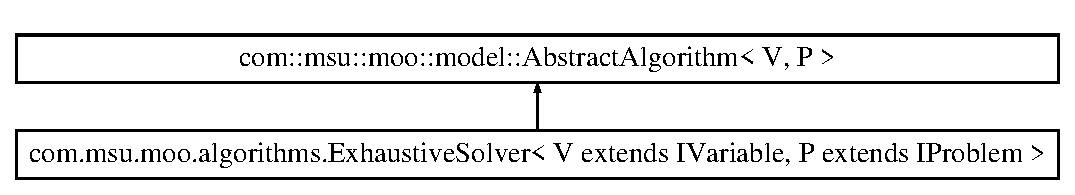
\includegraphics[height=2.000000cm]{classcom_1_1msu_1_1moo_1_1algorithms_1_1ExhaustiveSolver_3_01V_01extends_01IVariable_00_01P_01extends_01IProblem_01_4}
\end{center}
\end{figure}
\subsection*{Public Member Functions}
\begin{DoxyCompactItemize}
\item 
\hypertarget{classcom_1_1msu_1_1moo_1_1algorithms_1_1ExhaustiveSolver_3_01V_01extends_01IVariable_00_01P_01extends_01IProblem_01_4_adecccb0b347653f660431490c7256c00}{{\bfseries Exhaustive\-Solver} (Variable\-Factory$<$ V, P $>$ factory)}\label{classcom_1_1msu_1_1moo_1_1algorithms_1_1ExhaustiveSolver_3_01V_01extends_01IVariable_00_01P_01extends_01IProblem_01_4_adecccb0b347653f660431490c7256c00}

\item 
\hypertarget{classcom_1_1msu_1_1moo_1_1algorithms_1_1ExhaustiveSolver_3_01V_01extends_01IVariable_00_01P_01extends_01IProblem_01_4_ae8001f969408d4b41260ae762ea65169}{boolean {\bfseries has\-Finished} ()}\label{classcom_1_1msu_1_1moo_1_1algorithms_1_1ExhaustiveSolver_3_01V_01extends_01IVariable_00_01P_01extends_01IProblem_01_4_ae8001f969408d4b41260ae762ea65169}

\end{DoxyCompactItemize}
\subsection*{Protected Member Functions}
\begin{DoxyCompactItemize}
\item 
\hypertarget{classcom_1_1msu_1_1moo_1_1algorithms_1_1ExhaustiveSolver_3_01V_01extends_01IVariable_00_01P_01extends_01IProblem_01_4_a77e2ee35b6ec2be09f4ce566a56918a7}{void {\bfseries initialize} ()}\label{classcom_1_1msu_1_1moo_1_1algorithms_1_1ExhaustiveSolver_3_01V_01extends_01IVariable_00_01P_01extends_01IProblem_01_4_a77e2ee35b6ec2be09f4ce566a56918a7}

\item 
\hypertarget{classcom_1_1msu_1_1moo_1_1algorithms_1_1ExhaustiveSolver_3_01V_01extends_01IVariable_00_01P_01extends_01IProblem_01_4_af8152a2f383101cdb341c8e528c063e8}{void {\bfseries next} ()}\label{classcom_1_1msu_1_1moo_1_1algorithms_1_1ExhaustiveSolver_3_01V_01extends_01IVariable_00_01P_01extends_01IProblem_01_4_af8152a2f383101cdb341c8e528c063e8}

\item 
\hypertarget{classcom_1_1msu_1_1moo_1_1algorithms_1_1ExhaustiveSolver_3_01V_01extends_01IVariable_00_01P_01extends_01IProblem_01_4_a83de3f91fed2f57446488864b481e4b5}{\hyperlink{classcom_1_1msu_1_1moo_1_1model_1_1solution_1_1NonDominatedSolutionSet}{Non\-Dominated\-Solution\-Set} {\bfseries get\-Result} ()}\label{classcom_1_1msu_1_1moo_1_1algorithms_1_1ExhaustiveSolver_3_01V_01extends_01IVariable_00_01P_01extends_01IProblem_01_4_a83de3f91fed2f57446488864b481e4b5}

\end{DoxyCompactItemize}
\subsection*{Protected Attributes}
\begin{DoxyCompactItemize}
\item 
\hypertarget{classcom_1_1msu_1_1moo_1_1algorithms_1_1ExhaustiveSolver_3_01V_01extends_01IVariable_00_01P_01extends_01IProblem_01_4_a71615fa157f4d181101547c59d553e81}{\hyperlink{classcom_1_1msu_1_1moo_1_1model_1_1solution_1_1NonDominatedSolutionSet}{Non\-Dominated\-Solution\-Set} \hyperlink{classcom_1_1msu_1_1moo_1_1algorithms_1_1ExhaustiveSolver_3_01V_01extends_01IVariable_00_01P_01extends_01IProblem_01_4_a71615fa157f4d181101547c59d553e81}{set}}\label{classcom_1_1msu_1_1moo_1_1algorithms_1_1ExhaustiveSolver_3_01V_01extends_01IVariable_00_01P_01extends_01IProblem_01_4_a71615fa157f4d181101547c59d553e81}

\begin{DoxyCompactList}\small\item\em the final result set \end{DoxyCompactList}\item 
\hypertarget{classcom_1_1msu_1_1moo_1_1algorithms_1_1ExhaustiveSolver_3_01V_01extends_01IVariable_00_01P_01extends_01IProblem_01_4_a43dc999ee116079db5279c329eac8d82}{int \hyperlink{classcom_1_1msu_1_1moo_1_1algorithms_1_1ExhaustiveSolver_3_01V_01extends_01IVariable_00_01P_01extends_01IProblem_01_4_a43dc999ee116079db5279c329eac8d82}{evals\-Per\-Next} = 100}\label{classcom_1_1msu_1_1moo_1_1algorithms_1_1ExhaustiveSolver_3_01V_01extends_01IVariable_00_01P_01extends_01IProblem_01_4_a43dc999ee116079db5279c329eac8d82}

\begin{DoxyCompactList}\small\item\em how many evaluations per next \end{DoxyCompactList}\item 
\hypertarget{classcom_1_1msu_1_1moo_1_1algorithms_1_1ExhaustiveSolver_3_01V_01extends_01IVariable_00_01P_01extends_01IProblem_01_4_a13de3b464a86a794e2177a16cf24fe07}{boolean {\bfseries has\-Finished} = false}\label{classcom_1_1msu_1_1moo_1_1algorithms_1_1ExhaustiveSolver_3_01V_01extends_01IVariable_00_01P_01extends_01IProblem_01_4_a13de3b464a86a794e2177a16cf24fe07}

\end{DoxyCompactItemize}


\subsection{Detailed Description}
This solver iterates as long as the factory is not able to provide a new solution. It is up to the factory to exhaustive the whole search space! 

The documentation for this class was generated from the following file\-:\begin{DoxyCompactItemize}
\item 
src/main/java/com/msu/moo/algorithms/Exhaustive\-Solver.\-java\end{DoxyCompactItemize}

\hypertarget{classcom_1_1msu_1_1moo_1_1experiment_1_1ExperimentResult}{\section{com.\-msu.\-moo.\-experiment.\-Experiment\-Result Class Reference}
\label{classcom_1_1msu_1_1moo_1_1experiment_1_1ExperimentResult}\index{com.\-msu.\-moo.\-experiment.\-Experiment\-Result@{com.\-msu.\-moo.\-experiment.\-Experiment\-Result}}
}
\subsection*{Public Member Functions}
\begin{DoxyCompactItemize}
\item 
\hypertarget{classcom_1_1msu_1_1moo_1_1experiment_1_1ExperimentResult_a225f98f23ab87253bd91f037517aa43d}{void {\bfseries add} (\hyperlink{interfacecom_1_1msu_1_1moo_1_1model_1_1interfaces_1_1IProblem}{I\-Problem} problem, I\-Algorithm$<$?$>$ algorithm, \hyperlink{classcom_1_1msu_1_1moo_1_1model_1_1solution_1_1NonDominatedSolutionSet}{Non\-Dominated\-Solution\-Set} set)}\label{classcom_1_1msu_1_1moo_1_1experiment_1_1ExperimentResult_a225f98f23ab87253bd91f037517aa43d}

\item 
\hypertarget{classcom_1_1msu_1_1moo_1_1experiment_1_1ExperimentResult_ad5e42824165c0405debca2182e9cd8a6}{void {\bfseries add\-True\-Front} (\hyperlink{interfacecom_1_1msu_1_1moo_1_1model_1_1interfaces_1_1IProblem}{I\-Problem} problem, \hyperlink{classcom_1_1msu_1_1moo_1_1model_1_1solution_1_1NonDominatedSolutionSet}{Non\-Dominated\-Solution\-Set} set)}\label{classcom_1_1msu_1_1moo_1_1experiment_1_1ExperimentResult_ad5e42824165c0405debca2182e9cd8a6}

\item 
\hypertarget{classcom_1_1msu_1_1moo_1_1experiment_1_1ExperimentResult_afb01e5643dd559c8e8d59fa96d691572}{\hyperlink{classcom_1_1msu_1_1moo_1_1model_1_1solution_1_1NonDominatedSolutionSet}{Non\-Dominated\-Solution\-Set} {\bfseries get\-True\-Front} (\hyperlink{interfacecom_1_1msu_1_1moo_1_1model_1_1interfaces_1_1IProblem}{I\-Problem} problem)}\label{classcom_1_1msu_1_1moo_1_1experiment_1_1ExperimentResult_afb01e5643dd559c8e8d59fa96d691572}

\item 
\hypertarget{classcom_1_1msu_1_1moo_1_1experiment_1_1ExperimentResult_a4d691c059cd70f300640f4d25000e906}{String {\bfseries to\-String} ()}\label{classcom_1_1msu_1_1moo_1_1experiment_1_1ExperimentResult_a4d691c059cd70f300640f4d25000e906}

\item 
\hypertarget{classcom_1_1msu_1_1moo_1_1experiment_1_1ExperimentResult_a194d3ea8a71e110c658aed14854e1aad}{Multimap$<$ String, \\*
\hyperlink{classcom_1_1msu_1_1moo_1_1model_1_1solution_1_1NonDominatedSolutionSet}{Non\-Dominated\-Solution\-Set} $>$ {\bfseries get} ()}\label{classcom_1_1msu_1_1moo_1_1experiment_1_1ExperimentResult_a194d3ea8a71e110c658aed14854e1aad}

\item 
\hypertarget{classcom_1_1msu_1_1moo_1_1experiment_1_1ExperimentResult_a3a4d41e0bf3f059631ebab864b53b436}{Collection\\*
$<$ \hyperlink{classcom_1_1msu_1_1moo_1_1model_1_1solution_1_1NonDominatedSolutionSet}{Non\-Dominated\-Solution\-Set} $>$ {\bfseries get} (\hyperlink{interfacecom_1_1msu_1_1moo_1_1model_1_1interfaces_1_1IProblem}{I\-Problem} problem, I\-Algorithm$<$?$>$ algorithm)}\label{classcom_1_1msu_1_1moo_1_1experiment_1_1ExperimentResult_a3a4d41e0bf3f059631ebab864b53b436}

\end{DoxyCompactItemize}
\subsection*{Protected Attributes}
\begin{DoxyCompactItemize}
\item 
\hypertarget{classcom_1_1msu_1_1moo_1_1experiment_1_1ExperimentResult_afaccbbdd221d2fbbe9f2d7d7915b26c8}{Multimap$<$ String, \\*
\hyperlink{classcom_1_1msu_1_1moo_1_1model_1_1solution_1_1NonDominatedSolutionSet}{Non\-Dominated\-Solution\-Set} $>$ {\bfseries map} = Hash\-Multimap.\-create()}\label{classcom_1_1msu_1_1moo_1_1experiment_1_1ExperimentResult_afaccbbdd221d2fbbe9f2d7d7915b26c8}

\item 
\hypertarget{classcom_1_1msu_1_1moo_1_1experiment_1_1ExperimentResult_aa617707bfa9f7eb1766276a7cdd22413}{Map$<$ \hyperlink{interfacecom_1_1msu_1_1moo_1_1model_1_1interfaces_1_1IProblem}{I\-Problem}, \\*
\hyperlink{classcom_1_1msu_1_1moo_1_1model_1_1solution_1_1NonDominatedSolutionSet}{Non\-Dominated\-Solution\-Set} $>$ {\bfseries m\-True\-Fronts} = new Hash\-Map$<$$>$()}\label{classcom_1_1msu_1_1moo_1_1experiment_1_1ExperimentResult_aa617707bfa9f7eb1766276a7cdd22413}

\end{DoxyCompactItemize}


\subsection{Detailed Description}
This class is responsible to store all the fronts from the algorithms. Also during the max\-Evaluations time. 

The documentation for this class was generated from the following file\-:\begin{DoxyCompactItemize}
\item 
src/main/java/com/msu/moo/experiment/Experiment\-Result.\-java\end{DoxyCompactItemize}

\hypertarget{classcom_1_1msu_1_1moo_1_1fonseca_1_1FonsecaUtil}{\section{com.\-msu.\-moo.\-fonseca.\-Fonseca\-Util Class Reference}
\label{classcom_1_1msu_1_1moo_1_1fonseca_1_1FonsecaUtil}\index{com.\-msu.\-moo.\-fonseca.\-Fonseca\-Util@{com.\-msu.\-moo.\-fonseca.\-Fonseca\-Util}}
}
\subsection*{Static Public Member Functions}
\begin{DoxyCompactItemize}
\item 
\hypertarget{classcom_1_1msu_1_1moo_1_1fonseca_1_1FonsecaUtil_a4b8bdc4e76542bde4bfeba4a6fbbab63}{static String {\bfseries to\-String} (List$<$ Double $>$ l)}\label{classcom_1_1msu_1_1moo_1_1fonseca_1_1FonsecaUtil_a4b8bdc4e76542bde4bfeba4a6fbbab63}

\item 
\hypertarget{classcom_1_1msu_1_1moo_1_1fonseca_1_1FonsecaUtil_a7325063e612b58977b75f1d2a37cc5bb}{static String {\bfseries to\-String} (\hyperlink{classcom_1_1msu_1_1moo_1_1model_1_1solution_1_1SolutionSet}{Solution\-Set} set)}\label{classcom_1_1msu_1_1moo_1_1fonseca_1_1FonsecaUtil_a7325063e612b58977b75f1d2a37cc5bb}

\end{DoxyCompactItemize}


The documentation for this class was generated from the following file\-:\begin{DoxyCompactItemize}
\item 
src/main/java/com/msu/moo/fonseca/Fonseca\-Util.\-java\end{DoxyCompactItemize}

\hypertarget{classcom_1_1msu_1_1moo_1_1util_1_1FrontUtil}{\section{com.\-msu.\-moo.\-util.\-Front\-Util Class Reference}
\label{classcom_1_1msu_1_1moo_1_1util_1_1FrontUtil}\index{com.\-msu.\-moo.\-util.\-Front\-Util@{com.\-msu.\-moo.\-util.\-Front\-Util}}
}
\subsection*{Static Public Member Functions}
\begin{DoxyCompactItemize}
\item 
\hypertarget{classcom_1_1msu_1_1moo_1_1util_1_1FrontUtil_a1c7ece73360392eff06a2c4f1a45da86}{static$<$ Pextends\-I\-Problem $>$\\*
 \hyperlink{classcom_1_1msu_1_1moo_1_1model_1_1solution_1_1NonDominatedSolutionSet}{Non\-Dominated\-Solution\-Set} {\bfseries estimate\-True\-Front} (Map$<$ I\-Algorithm$<$ P $>$, List$<$ \hyperlink{classcom_1_1msu_1_1moo_1_1model_1_1solution_1_1NonDominatedSolutionSet}{Non\-Dominated\-Solution\-Set} $>$$>$ fronts)}\label{classcom_1_1msu_1_1moo_1_1util_1_1FrontUtil_a1c7ece73360392eff06a2c4f1a45da86}

\item 
\hypertarget{classcom_1_1msu_1_1moo_1_1util_1_1FrontUtil_a232bcf75274796befbc241c1dcc30889}{static$<$ Pextends\-I\-Problem $>$\\*
 \hyperlink{classcom_1_1msu_1_1moo_1_1visualization_1_1ScatterPlot}{Scatter\-Plot} {\bfseries create\-Scatter\-Plot} (String title, Map$<$ I\-Algorithm$<$ P $>$, \hyperlink{classcom_1_1msu_1_1moo_1_1model_1_1solution_1_1NonDominatedSolutionSet}{Non\-Dominated\-Solution\-Set} $>$ fronts)}\label{classcom_1_1msu_1_1moo_1_1util_1_1FrontUtil_a232bcf75274796befbc241c1dcc30889}

\item 
\hypertarget{classcom_1_1msu_1_1moo_1_1util_1_1FrontUtil_ae6be14fc492457191afc6c9d5af0383e}{static$<$ Pextends\-I\-Problem $>$ \hyperlink{classcom_1_1msu_1_1moo_1_1visualization_1_1BoxPlot}{Box\-Plot} {\bfseries create\-Box\-Plot} (String title, Map$<$ I\-Algorithm$<$ P $>$, List$<$ Double $>$$>$ hv\-Map)}\label{classcom_1_1msu_1_1moo_1_1util_1_1FrontUtil_ae6be14fc492457191afc6c9d5af0383e}

\item 
\hypertarget{classcom_1_1msu_1_1moo_1_1util_1_1FrontUtil_a88acca7b870b4fbff9b31d16f2a03e38}{static$<$ Pextends\-I\-Problem $>$ Map\\*
$<$ I\-Algorithm$<$ P $>$\\*
, \hyperlink{classcom_1_1msu_1_1moo_1_1model_1_1solution_1_1NonDominatedSolutionSet}{Non\-Dominated\-Solution\-Set} $>$ {\bfseries calc\-Median\-Fronts} (Map$<$ I\-Algorithm$<$ P $>$, List$<$ \hyperlink{classcom_1_1msu_1_1moo_1_1model_1_1solution_1_1NonDominatedSolutionSet}{Non\-Dominated\-Solution\-Set} $>$$>$ fronts, String path\-To\-E\-A\-F)}\label{classcom_1_1msu_1_1moo_1_1util_1_1FrontUtil_a88acca7b870b4fbff9b31d16f2a03e38}

\item 
\hypertarget{classcom_1_1msu_1_1moo_1_1util_1_1FrontUtil_aa26ee0f69a08dcd6026bd27c6194e214}{static$<$ Pextends\-I\-Problem $>$ Map\\*
$<$ I\-Algorithm$<$ P $>$, List\\*
$<$ Double $>$ $>$ {\bfseries calc\-Hypervolume} (\hyperlink{classcom_1_1msu_1_1moo_1_1model_1_1solution_1_1NonDominatedSolutionSet}{Non\-Dominated\-Solution\-Set} true\-Front, Map$<$ I\-Algorithm$<$ P $>$, List$<$ \hyperlink{classcom_1_1msu_1_1moo_1_1model_1_1solution_1_1NonDominatedSolutionSet}{Non\-Dominated\-Solution\-Set} $>$$>$ all\-Fronts, String path\-To\-H\-V)}\label{classcom_1_1msu_1_1moo_1_1util_1_1FrontUtil_aa26ee0f69a08dcd6026bd27c6194e214}

\end{DoxyCompactItemize}


The documentation for this class was generated from the following file\-:\begin{DoxyCompactItemize}
\item 
src/main/java/com/msu/moo/util/Front\-Util.\-java\end{DoxyCompactItemize}

\hypertarget{classcom_1_1msu_1_1moo_1_1operators_1_1crossover_1_1HalfUniformCrossover_3_01T_01_4}{\section{com.\-msu.\-moo.\-operators.\-crossover.\-Half\-Uniform\-Crossover$<$ T $>$ Class Reference}
\label{classcom_1_1msu_1_1moo_1_1operators_1_1crossover_1_1HalfUniformCrossover_3_01T_01_4}\index{com.\-msu.\-moo.\-operators.\-crossover.\-Half\-Uniform\-Crossover$<$ T $>$@{com.\-msu.\-moo.\-operators.\-crossover.\-Half\-Uniform\-Crossover$<$ T $>$}}
}
Inheritance diagram for com.\-msu.\-moo.\-operators.\-crossover.\-Half\-Uniform\-Crossover$<$ T $>$\-:\begin{figure}[H]
\begin{center}
\leavevmode
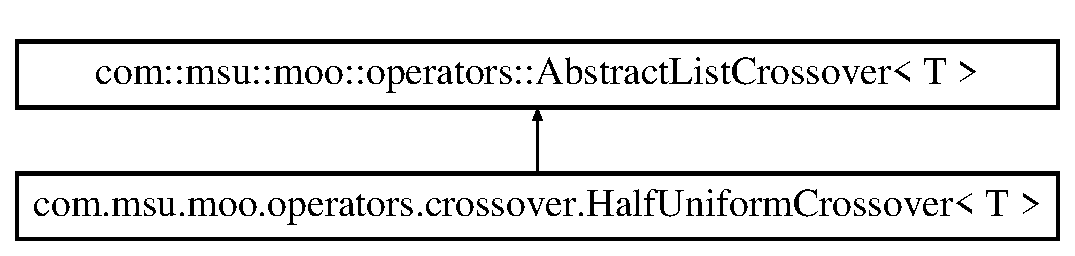
\includegraphics[height=2.000000cm]{classcom_1_1msu_1_1moo_1_1operators_1_1crossover_1_1HalfUniformCrossover_3_01T_01_4}
\end{center}
\end{figure}
\subsection*{Protected Member Functions}
\begin{DoxyCompactItemize}
\item 
List$<$ Integer $>$ \hyperlink{classcom_1_1msu_1_1moo_1_1operators_1_1crossover_1_1HalfUniformCrossover_3_01T_01_4_af0ecb25efc748432acac34064f146b9a}{get\-Not\-Equal\-Indices} (List$<$ T $>$ a, List$<$ T $>$ b)
\item 
\hypertarget{classcom_1_1msu_1_1moo_1_1operators_1_1crossover_1_1HalfUniformCrossover_3_01T_01_4_acbc99967d8180a9ed309686b54f418dd}{List$<$ List$<$ T $>$ $>$ {\bfseries crossover\-Lists} (List$<$ T $>$ a, List$<$ T $>$ b)}\label{classcom_1_1msu_1_1moo_1_1operators_1_1crossover_1_1HalfUniformCrossover_3_01T_01_4_acbc99967d8180a9ed309686b54f418dd}

\end{DoxyCompactItemize}


\subsection{Member Function Documentation}
\hypertarget{classcom_1_1msu_1_1moo_1_1operators_1_1crossover_1_1HalfUniformCrossover_3_01T_01_4_af0ecb25efc748432acac34064f146b9a}{\index{com\-::msu\-::moo\-::operators\-::crossover\-::\-Half\-Uniform\-Crossover$<$ T $>$@{com\-::msu\-::moo\-::operators\-::crossover\-::\-Half\-Uniform\-Crossover$<$ T $>$}!get\-Not\-Equal\-Indices@{get\-Not\-Equal\-Indices}}
\index{get\-Not\-Equal\-Indices@{get\-Not\-Equal\-Indices}!com::msu::moo::operators::crossover::HalfUniformCrossover< T >@{com\-::msu\-::moo\-::operators\-::crossover\-::\-Half\-Uniform\-Crossover$<$ T $>$}}
\subsubsection[{get\-Not\-Equal\-Indices}]{\setlength{\rightskip}{0pt plus 5cm}List$<$Integer$>$ com.\-msu.\-moo.\-operators.\-crossover.\-Half\-Uniform\-Crossover$<$ T $>$.get\-Not\-Equal\-Indices (
\begin{DoxyParamCaption}
\item[{List$<$ T $>$}]{a, }
\item[{List$<$ T $>$}]{b}
\end{DoxyParamCaption}
)\hspace{0.3cm}{\ttfamily [inline]}, {\ttfamily [protected]}}}\label{classcom_1_1msu_1_1moo_1_1operators_1_1crossover_1_1HalfUniformCrossover_3_01T_01_4_af0ecb25efc748432acac34064f146b9a}
Returns all the positions that are different at the two parents.

\begin{DoxyReturn}{Returns}
all indices that are different! 
\end{DoxyReturn}


The documentation for this class was generated from the following file\-:\begin{DoxyCompactItemize}
\item 
src/main/java/com/msu/moo/operators/crossover/Half\-Uniform\-Crossover.\-java\end{DoxyCompactItemize}

\hypertarget{classcom_1_1msu_1_1moo_1_1fonseca_1_1Hypervolume}{\section{com.\-msu.\-moo.\-fonseca.\-Hypervolume Class Reference}
\label{classcom_1_1msu_1_1moo_1_1fonseca_1_1Hypervolume}\index{com.\-msu.\-moo.\-fonseca.\-Hypervolume@{com.\-msu.\-moo.\-fonseca.\-Hypervolume}}
}
\subsection*{Public Member Functions}
\begin{DoxyCompactItemize}
\item 
\hypertarget{classcom_1_1msu_1_1moo_1_1fonseca_1_1Hypervolume_af3065d83378f830c67e6353aa639bed2}{{\bfseries Hypervolume} (String path\-To\-H\-V)}\label{classcom_1_1msu_1_1moo_1_1fonseca_1_1Hypervolume_af3065d83378f830c67e6353aa639bed2}

\item 
\hypertarget{classcom_1_1msu_1_1moo_1_1fonseca_1_1Hypervolume_ae96f9b9409bc84cef00ef85ce7620c90}{Double {\bfseries calculate} (\hyperlink{classcom_1_1msu_1_1moo_1_1model_1_1solution_1_1NonDominatedSolutionSet}{Non\-Dominated\-Solution\-Set} set)}\label{classcom_1_1msu_1_1moo_1_1fonseca_1_1Hypervolume_ae96f9b9409bc84cef00ef85ce7620c90}

\item 
\hypertarget{classcom_1_1msu_1_1moo_1_1fonseca_1_1Hypervolume_aa983676f2bb3b019c55f1f640b0755e7}{Double {\bfseries calculate} (\hyperlink{classcom_1_1msu_1_1moo_1_1model_1_1solution_1_1NonDominatedSolutionSet}{Non\-Dominated\-Solution\-Set} set, List$<$ Double $>$ reference\-Point)}\label{classcom_1_1msu_1_1moo_1_1fonseca_1_1Hypervolume_aa983676f2bb3b019c55f1f640b0755e7}

\end{DoxyCompactItemize}
\subsection*{Protected Member Functions}
\begin{DoxyCompactItemize}
\item 
\hypertarget{classcom_1_1msu_1_1moo_1_1fonseca_1_1Hypervolume_af5fd4d955941d911bad0884bab5ccaaf}{String {\bfseries get\-Command} (\hyperlink{classcom_1_1msu_1_1moo_1_1model_1_1solution_1_1NonDominatedSolutionSet}{Non\-Dominated\-Solution\-Set} set)}\label{classcom_1_1msu_1_1moo_1_1fonseca_1_1Hypervolume_af5fd4d955941d911bad0884bab5ccaaf}

\end{DoxyCompactItemize}
\subsection*{Protected Attributes}
\begin{DoxyCompactItemize}
\item 
\hypertarget{classcom_1_1msu_1_1moo_1_1fonseca_1_1Hypervolume_ab46095cd7c8a905b334478665996ce1f}{String {\bfseries path\-To\-H\-V} = null}\label{classcom_1_1msu_1_1moo_1_1fonseca_1_1Hypervolume_ab46095cd7c8a905b334478665996ce1f}

\end{DoxyCompactItemize}


The documentation for this class was generated from the following file\-:\begin{DoxyCompactItemize}
\item 
src/main/java/com/msu/moo/fonseca/Hypervolume.\-java\end{DoxyCompactItemize}

\hypertarget{interfacecom_1_1msu_1_1moo_1_1model_1_1interfaces_1_1IAlgorithm_3_01P_01extends_01IProblem_01_4}{\section{com.\-msu.\-moo.\-model.\-interfaces.\-I\-Algorithm$<$ P extends I\-Problem $>$ Interface Reference}
\label{interfacecom_1_1msu_1_1moo_1_1model_1_1interfaces_1_1IAlgorithm_3_01P_01extends_01IProblem_01_4}\index{com.\-msu.\-moo.\-model.\-interfaces.\-I\-Algorithm$<$ P extends I\-Problem $>$@{com.\-msu.\-moo.\-model.\-interfaces.\-I\-Algorithm$<$ P extends I\-Problem $>$}}
}
\subsection*{Public Member Functions}
\begin{DoxyCompactItemize}
\item 
\hyperlink{classcom_1_1msu_1_1moo_1_1model_1_1solution_1_1NonDominatedSolutionSet}{Non\-Dominated\-Solution\-Set} \hyperlink{interfacecom_1_1msu_1_1moo_1_1model_1_1interfaces_1_1IAlgorithm_3_01P_01extends_01IProblem_01_4_ad53bbbe3ea9a341b7bbf3a0104ca5315}{run} (P problem)
\item 
void \hyperlink{interfacecom_1_1msu_1_1moo_1_1model_1_1interfaces_1_1IAlgorithm_3_01P_01extends_01IProblem_01_4_a3114ec28cb5b0d2c4a8b5adef1932226}{set\-Max\-Evaluations} (long n)
\item 
Map$<$ Long, \\*
\hyperlink{classcom_1_1msu_1_1moo_1_1model_1_1solution_1_1NonDominatedSolutionSet}{Non\-Dominated\-Solution\-Set} $>$ \hyperlink{interfacecom_1_1msu_1_1moo_1_1model_1_1interfaces_1_1IAlgorithm_3_01P_01extends_01IProblem_01_4_a7b74b82fd1813895e5e741c9bb254c7b}{get\-History} ()
\item 
String \hyperlink{interfacecom_1_1msu_1_1moo_1_1model_1_1interfaces_1_1IAlgorithm_3_01P_01extends_01IProblem_01_4_a9b2e6160ffd2274fa75018c18b6580d2}{get\-Name} ()
\item 
void \hyperlink{interfacecom_1_1msu_1_1moo_1_1model_1_1interfaces_1_1IAlgorithm_3_01P_01extends_01IProblem_01_4_ab6d0d14d4349dedcad8eb083b0ce5f75}{set\-Name} (String name)
\end{DoxyCompactItemize}


\subsection{Member Function Documentation}
\hypertarget{interfacecom_1_1msu_1_1moo_1_1model_1_1interfaces_1_1IAlgorithm_3_01P_01extends_01IProblem_01_4_a7b74b82fd1813895e5e741c9bb254c7b}{\index{com\-::msu\-::moo\-::model\-::interfaces\-::\-I\-Algorithm$<$ P extends I\-Problem $>$@{com\-::msu\-::moo\-::model\-::interfaces\-::\-I\-Algorithm$<$ P extends I\-Problem $>$}!get\-History@{get\-History}}
\index{get\-History@{get\-History}!com::msu::moo::model::interfaces::IAlgorithm< P extends IProblem >@{com\-::msu\-::moo\-::model\-::interfaces\-::\-I\-Algorithm$<$ P extends I\-Problem $>$}}
\subsubsection[{get\-History}]{\setlength{\rightskip}{0pt plus 5cm}Map$<$Long, {\bf Non\-Dominated\-Solution\-Set}$>$ com.\-msu.\-moo.\-model.\-interfaces.\-I\-Algorithm$<$ P extends {\bf I\-Problem} $>$.get\-History (
\begin{DoxyParamCaption}
{}
\end{DoxyParamCaption}
)}}\label{interfacecom_1_1msu_1_1moo_1_1model_1_1interfaces_1_1IAlgorithm_3_01P_01extends_01IProblem_01_4_a7b74b82fd1813895e5e741c9bb254c7b}
\begin{DoxyReturn}{Returns}
all the history values of the algorithms 
\end{DoxyReturn}
\hypertarget{interfacecom_1_1msu_1_1moo_1_1model_1_1interfaces_1_1IAlgorithm_3_01P_01extends_01IProblem_01_4_a9b2e6160ffd2274fa75018c18b6580d2}{\index{com\-::msu\-::moo\-::model\-::interfaces\-::\-I\-Algorithm$<$ P extends I\-Problem $>$@{com\-::msu\-::moo\-::model\-::interfaces\-::\-I\-Algorithm$<$ P extends I\-Problem $>$}!get\-Name@{get\-Name}}
\index{get\-Name@{get\-Name}!com::msu::moo::model::interfaces::IAlgorithm< P extends IProblem >@{com\-::msu\-::moo\-::model\-::interfaces\-::\-I\-Algorithm$<$ P extends I\-Problem $>$}}
\subsubsection[{get\-Name}]{\setlength{\rightskip}{0pt plus 5cm}String com.\-msu.\-moo.\-model.\-interfaces.\-I\-Algorithm$<$ P extends {\bf I\-Problem} $>$.get\-Name (
\begin{DoxyParamCaption}
{}
\end{DoxyParamCaption}
)}}\label{interfacecom_1_1msu_1_1moo_1_1model_1_1interfaces_1_1IAlgorithm_3_01P_01extends_01IProblem_01_4_a9b2e6160ffd2274fa75018c18b6580d2}
\begin{DoxyReturn}{Returns}
the name of this algorithm or instance with different parameters 
\end{DoxyReturn}
\hypertarget{interfacecom_1_1msu_1_1moo_1_1model_1_1interfaces_1_1IAlgorithm_3_01P_01extends_01IProblem_01_4_ad53bbbe3ea9a341b7bbf3a0104ca5315}{\index{com\-::msu\-::moo\-::model\-::interfaces\-::\-I\-Algorithm$<$ P extends I\-Problem $>$@{com\-::msu\-::moo\-::model\-::interfaces\-::\-I\-Algorithm$<$ P extends I\-Problem $>$}!run@{run}}
\index{run@{run}!com::msu::moo::model::interfaces::IAlgorithm< P extends IProblem >@{com\-::msu\-::moo\-::model\-::interfaces\-::\-I\-Algorithm$<$ P extends I\-Problem $>$}}
\subsubsection[{run}]{\setlength{\rightskip}{0pt plus 5cm}{\bf Non\-Dominated\-Solution\-Set} com.\-msu.\-moo.\-model.\-interfaces.\-I\-Algorithm$<$ P extends {\bf I\-Problem} $>$.run (
\begin{DoxyParamCaption}
\item[{P}]{problem}
\end{DoxyParamCaption}
)}}\label{interfacecom_1_1msu_1_1moo_1_1model_1_1interfaces_1_1IAlgorithm_3_01P_01extends_01IProblem_01_4_ad53bbbe3ea9a341b7bbf3a0104ca5315}
Execute the algorithm.


\begin{DoxyParams}{Parameters}
{\em problem} & instance of the problem \\
\hline
\end{DoxyParams}
\begin{DoxyReturn}{Returns}
Non\-Dominted\-Set which was calculated 
\end{DoxyReturn}
\hypertarget{interfacecom_1_1msu_1_1moo_1_1model_1_1interfaces_1_1IAlgorithm_3_01P_01extends_01IProblem_01_4_a3114ec28cb5b0d2c4a8b5adef1932226}{\index{com\-::msu\-::moo\-::model\-::interfaces\-::\-I\-Algorithm$<$ P extends I\-Problem $>$@{com\-::msu\-::moo\-::model\-::interfaces\-::\-I\-Algorithm$<$ P extends I\-Problem $>$}!set\-Max\-Evaluations@{set\-Max\-Evaluations}}
\index{set\-Max\-Evaluations@{set\-Max\-Evaluations}!com::msu::moo::model::interfaces::IAlgorithm< P extends IProblem >@{com\-::msu\-::moo\-::model\-::interfaces\-::\-I\-Algorithm$<$ P extends I\-Problem $>$}}
\subsubsection[{set\-Max\-Evaluations}]{\setlength{\rightskip}{0pt plus 5cm}void com.\-msu.\-moo.\-model.\-interfaces.\-I\-Algorithm$<$ P extends {\bf I\-Problem} $>$.set\-Max\-Evaluations (
\begin{DoxyParamCaption}
\item[{long}]{n}
\end{DoxyParamCaption}
)}}\label{interfacecom_1_1msu_1_1moo_1_1model_1_1interfaces_1_1IAlgorithm_3_01P_01extends_01IProblem_01_4_a3114ec28cb5b0d2c4a8b5adef1932226}
\begin{DoxyReturn}{Returns}
maximal number of evaluations that should be allowed 
\end{DoxyReturn}
\hypertarget{interfacecom_1_1msu_1_1moo_1_1model_1_1interfaces_1_1IAlgorithm_3_01P_01extends_01IProblem_01_4_ab6d0d14d4349dedcad8eb083b0ce5f75}{\index{com\-::msu\-::moo\-::model\-::interfaces\-::\-I\-Algorithm$<$ P extends I\-Problem $>$@{com\-::msu\-::moo\-::model\-::interfaces\-::\-I\-Algorithm$<$ P extends I\-Problem $>$}!set\-Name@{set\-Name}}
\index{set\-Name@{set\-Name}!com::msu::moo::model::interfaces::IAlgorithm< P extends IProblem >@{com\-::msu\-::moo\-::model\-::interfaces\-::\-I\-Algorithm$<$ P extends I\-Problem $>$}}
\subsubsection[{set\-Name}]{\setlength{\rightskip}{0pt plus 5cm}void com.\-msu.\-moo.\-model.\-interfaces.\-I\-Algorithm$<$ P extends {\bf I\-Problem} $>$.set\-Name (
\begin{DoxyParamCaption}
\item[{String}]{name}
\end{DoxyParamCaption}
)}}\label{interfacecom_1_1msu_1_1moo_1_1model_1_1interfaces_1_1IAlgorithm_3_01P_01extends_01IProblem_01_4_ab6d0d14d4349dedcad8eb083b0ce5f75}

\begin{DoxyParams}{Parameters}
{\em name} & for this algorithm \\
\hline
\end{DoxyParams}


The documentation for this interface was generated from the following file\-:\begin{DoxyCompactItemize}
\item 
src/main/java/com/msu/moo/model/interfaces/I\-Algorithm.\-java\end{DoxyCompactItemize}

\hypertarget{interfacecom_1_1msu_1_1moo_1_1model_1_1interfaces_1_1IFactory_3_01T_01extends_01IVariable_01_4}{\section{com.\-msu.\-moo.\-model.\-interfaces.\-I\-Factory$<$ T extends I\-Variable $>$ Interface Reference}
\label{interfacecom_1_1msu_1_1moo_1_1model_1_1interfaces_1_1IFactory_3_01T_01extends_01IVariable_01_4}\index{com.\-msu.\-moo.\-model.\-interfaces.\-I\-Factory$<$ T extends I\-Variable $>$@{com.\-msu.\-moo.\-model.\-interfaces.\-I\-Factory$<$ T extends I\-Variable $>$}}
}
\subsection*{Public Member Functions}
\begin{DoxyCompactItemize}
\item 
T \hyperlink{interfacecom_1_1msu_1_1moo_1_1model_1_1interfaces_1_1IFactory_3_01T_01extends_01IVariable_01_4_a6e9e257f9a813fed3795b42198e15255}{create} ()
\end{DoxyCompactItemize}


\subsection{Detailed Description}
This class represents a factory class that could construct new variable randomly.


\begin{DoxyParams}{Parameters}
{\em $<$\-T$>$} & variable type \\
\hline
\end{DoxyParams}


\subsection{Member Function Documentation}
\hypertarget{interfacecom_1_1msu_1_1moo_1_1model_1_1interfaces_1_1IFactory_3_01T_01extends_01IVariable_01_4_a6e9e257f9a813fed3795b42198e15255}{\index{com\-::msu\-::moo\-::model\-::interfaces\-::\-I\-Factory$<$ T extends I\-Variable $>$@{com\-::msu\-::moo\-::model\-::interfaces\-::\-I\-Factory$<$ T extends I\-Variable $>$}!create@{create}}
\index{create@{create}!com::msu::moo::model::interfaces::IFactory< T extends IVariable >@{com\-::msu\-::moo\-::model\-::interfaces\-::\-I\-Factory$<$ T extends I\-Variable $>$}}
\subsubsection[{create}]{\setlength{\rightskip}{0pt plus 5cm}T com.\-msu.\-moo.\-model.\-interfaces.\-I\-Factory$<$ T extends {\bf I\-Variable} $>$.create (
\begin{DoxyParamCaption}
{}
\end{DoxyParamCaption}
)}}\label{interfacecom_1_1msu_1_1moo_1_1model_1_1interfaces_1_1IFactory_3_01T_01extends_01IVariable_01_4_a6e9e257f9a813fed3795b42198e15255}
Create a new object from the class. \begin{DoxyReturn}{Returns}
new random instance. 
\end{DoxyReturn}


The documentation for this interface was generated from the following file\-:\begin{DoxyCompactItemize}
\item 
src/main/java/com/msu/moo/model/interfaces/I\-Factory.\-java\end{DoxyCompactItemize}

\hypertarget{classcom_1_1msu_1_1moo_1_1util_1_1indicator_1_1Indicator_3_01T_01_4}{\section{com.\-msu.\-moo.\-util.\-indicator.\-Indicator$<$ T $>$ Class Reference}
\label{classcom_1_1msu_1_1moo_1_1util_1_1indicator_1_1Indicator_3_01T_01_4}\index{com.\-msu.\-moo.\-util.\-indicator.\-Indicator$<$ T $>$@{com.\-msu.\-moo.\-util.\-indicator.\-Indicator$<$ T $>$}}
}
\subsection*{Public Member Functions}
\begin{DoxyCompactItemize}
\item 
Map$<$ \hyperlink{classcom_1_1msu_1_1moo_1_1model_1_1solution_1_1Solution}{Solution}, T $>$ \hyperlink{classcom_1_1msu_1_1moo_1_1util_1_1indicator_1_1Indicator_3_01T_01_4_ae3ab82087a1693527e8efb67d505d9c9}{calculate} (\hyperlink{classcom_1_1msu_1_1moo_1_1model_1_1solution_1_1SolutionSet}{Solution\-Set} solutions)
\item 
abstract void \hyperlink{classcom_1_1msu_1_1moo_1_1util_1_1indicator_1_1Indicator_3_01T_01_4_abcaeb04edbfd93448aacd930dee06b49}{calculate} (Map$<$ \hyperlink{classcom_1_1msu_1_1moo_1_1model_1_1solution_1_1Solution}{Solution}, T $>$ map, \hyperlink{classcom_1_1msu_1_1moo_1_1model_1_1solution_1_1SolutionSet}{Solution\-Set} solutions)
\end{DoxyCompactItemize}


\subsection{Detailed Description}
This provides a standardized class for indicator that could return in principle any type.


\begin{DoxyParams}{Parameters}
{\em $<$\-T$>$} & type of the result of indicator \\
\hline
\end{DoxyParams}


\subsection{Member Function Documentation}
\hypertarget{classcom_1_1msu_1_1moo_1_1util_1_1indicator_1_1Indicator_3_01T_01_4_ae3ab82087a1693527e8efb67d505d9c9}{\index{com\-::msu\-::moo\-::util\-::indicator\-::\-Indicator$<$ T $>$@{com\-::msu\-::moo\-::util\-::indicator\-::\-Indicator$<$ T $>$}!calculate@{calculate}}
\index{calculate@{calculate}!com::msu::moo::util::indicator::Indicator< T >@{com\-::msu\-::moo\-::util\-::indicator\-::\-Indicator$<$ T $>$}}
\subsubsection[{calculate}]{\setlength{\rightskip}{0pt plus 5cm}Map$<${\bf Solution}, T$>$ com.\-msu.\-moo.\-util.\-indicator.\-Indicator$<$ T $>$.calculate (
\begin{DoxyParamCaption}
\item[{{\bf Solution\-Set}}]{solutions}
\end{DoxyParamCaption}
)\hspace{0.3cm}{\ttfamily [inline]}}}\label{classcom_1_1msu_1_1moo_1_1util_1_1indicator_1_1Indicator_3_01T_01_4_ae3ab82087a1693527e8efb67d505d9c9}
Calculate indicator values and return a map with with result. \hypertarget{classcom_1_1msu_1_1moo_1_1util_1_1indicator_1_1Indicator_3_01T_01_4_abcaeb04edbfd93448aacd930dee06b49}{\index{com\-::msu\-::moo\-::util\-::indicator\-::\-Indicator$<$ T $>$@{com\-::msu\-::moo\-::util\-::indicator\-::\-Indicator$<$ T $>$}!calculate@{calculate}}
\index{calculate@{calculate}!com::msu::moo::util::indicator::Indicator< T >@{com\-::msu\-::moo\-::util\-::indicator\-::\-Indicator$<$ T $>$}}
\subsubsection[{calculate}]{\setlength{\rightskip}{0pt plus 5cm}abstract void com.\-msu.\-moo.\-util.\-indicator.\-Indicator$<$ T $>$.calculate (
\begin{DoxyParamCaption}
\item[{Map$<$ {\bf Solution}, T $>$}]{map, }
\item[{{\bf Solution\-Set}}]{solutions}
\end{DoxyParamCaption}
)\hspace{0.3cm}{\ttfamily [abstract]}}}\label{classcom_1_1msu_1_1moo_1_1util_1_1indicator_1_1Indicator_3_01T_01_4_abcaeb04edbfd93448aacd930dee06b49}
Add the result to the given map. 

The documentation for this class was generated from the following file\-:\begin{DoxyCompactItemize}
\item 
src/main/java/com/msu/moo/util/indicator/Indicator.\-java\end{DoxyCompactItemize}

\hypertarget{interfacecom_1_1msu_1_1moo_1_1visualization_1_1IPlot}{\section{com.\-msu.\-moo.\-visualization.\-I\-Plot Interface Reference}
\label{interfacecom_1_1msu_1_1moo_1_1visualization_1_1IPlot}\index{com.\-msu.\-moo.\-visualization.\-I\-Plot@{com.\-msu.\-moo.\-visualization.\-I\-Plot}}
}
Inheritance diagram for com.\-msu.\-moo.\-visualization.\-I\-Plot\-:\begin{figure}[H]
\begin{center}
\leavevmode
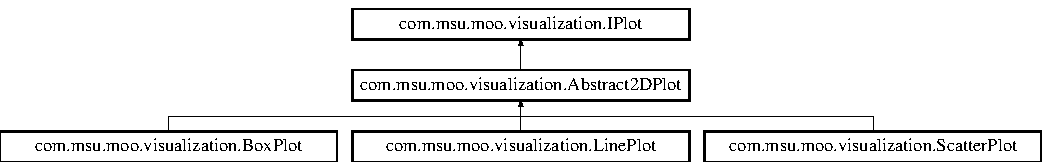
\includegraphics[height=2.178988cm]{interfacecom_1_1msu_1_1moo_1_1visualization_1_1IPlot}
\end{center}
\end{figure}
\subsection*{Public Member Functions}
\begin{DoxyCompactItemize}
\item 
J\-Free\-Chart \hyperlink{interfacecom_1_1msu_1_1moo_1_1visualization_1_1IPlot_ae45c2987d112fbf5bc5af7864fb50ecd}{get\-Chart} ()
\end{DoxyCompactItemize}


\subsection{Member Function Documentation}
\hypertarget{interfacecom_1_1msu_1_1moo_1_1visualization_1_1IPlot_ae45c2987d112fbf5bc5af7864fb50ecd}{\index{com\-::msu\-::moo\-::visualization\-::\-I\-Plot@{com\-::msu\-::moo\-::visualization\-::\-I\-Plot}!get\-Chart@{get\-Chart}}
\index{get\-Chart@{get\-Chart}!com::msu::moo::visualization::IPlot@{com\-::msu\-::moo\-::visualization\-::\-I\-Plot}}
\subsubsection[{get\-Chart}]{\setlength{\rightskip}{0pt plus 5cm}J\-Free\-Chart com.\-msu.\-moo.\-visualization.\-I\-Plot.\-get\-Chart (
\begin{DoxyParamCaption}
{}
\end{DoxyParamCaption}
)}}\label{interfacecom_1_1msu_1_1moo_1_1visualization_1_1IPlot_ae45c2987d112fbf5bc5af7864fb50ecd}
Every Plot needs the chart frame to visualize the results \begin{DoxyReturn}{Returns}
chart frame to make it visible 
\end{DoxyReturn}


Implemented in \hyperlink{classcom_1_1msu_1_1moo_1_1visualization_1_1ScatterPlot_a1c5117bd94b91e9ae2f59c1c025b243b}{com.\-msu.\-moo.\-visualization.\-Scatter\-Plot}, \hyperlink{classcom_1_1msu_1_1moo_1_1visualization_1_1LinePlot_ab6bc90e83277d08e59c3efd82e3b585d}{com.\-msu.\-moo.\-visualization.\-Line\-Plot}, and \hyperlink{classcom_1_1msu_1_1moo_1_1visualization_1_1BoxPlot_acfbffc8df459e92c6b39108371fd462c}{com.\-msu.\-moo.\-visualization.\-Box\-Plot}.



The documentation for this interface was generated from the following file\-:\begin{DoxyCompactItemize}
\item 
src/main/java/com/msu/moo/visualization/I\-Plot.\-java\end{DoxyCompactItemize}

\hypertarget{interfacecom_1_1msu_1_1moo_1_1model_1_1interfaces_1_1IProblem}{\section{com.\-msu.\-moo.\-model.\-interfaces.\-I\-Problem Interface Reference}
\label{interfacecom_1_1msu_1_1moo_1_1model_1_1interfaces_1_1IProblem}\index{com.\-msu.\-moo.\-model.\-interfaces.\-I\-Problem@{com.\-msu.\-moo.\-model.\-interfaces.\-I\-Problem}}
}
Inheritance diagram for com.\-msu.\-moo.\-model.\-interfaces.\-I\-Problem\-:\begin{figure}[H]
\begin{center}
\leavevmode
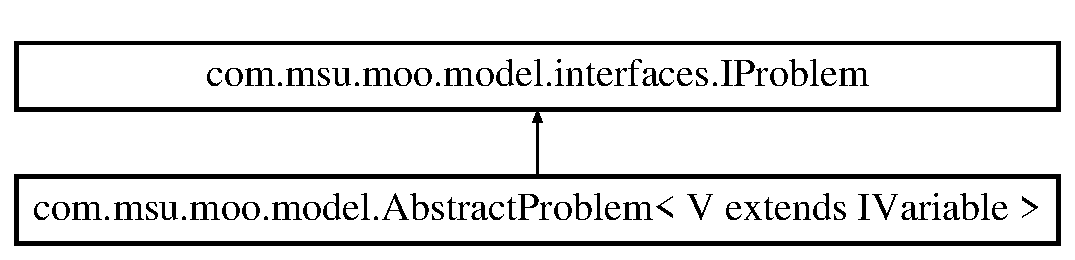
\includegraphics[height=2.000000cm]{interfacecom_1_1msu_1_1moo_1_1model_1_1interfaces_1_1IProblem}
\end{center}
\end{figure}
\subsection*{Public Member Functions}
\begin{DoxyCompactItemize}
\item 
\hyperlink{classcom_1_1msu_1_1moo_1_1model_1_1solution_1_1Solution}{Solution} \hyperlink{interfacecom_1_1msu_1_1moo_1_1model_1_1interfaces_1_1IProblem_a1ac7c52476b19b10a1e167551b9ead19}{evaluate} (\hyperlink{interfacecom_1_1msu_1_1moo_1_1model_1_1interfaces_1_1IVariable}{I\-Variable} variable)
\item 
long \hyperlink{interfacecom_1_1msu_1_1moo_1_1model_1_1interfaces_1_1IProblem_ad7dba60e3a3412017890543d3a0250b8}{get\-Num\-Of\-Evaluations} ()
\item 
void \hyperlink{interfacecom_1_1msu_1_1moo_1_1model_1_1interfaces_1_1IProblem_aca88ee486dcb7d96a218e76ea5034522}{reset} ()
\item 
int \hyperlink{interfacecom_1_1msu_1_1moo_1_1model_1_1interfaces_1_1IProblem_a3cac50c0c388545d9c70ac6893911c9f}{get\-Number\-Of\-Objectives} ()
\end{DoxyCompactItemize}


\subsection{Detailed Description}
This interface defines the values of a problem.

Each problem needs to have a evaluation method that has a predefined input I and output o


\begin{DoxyParams}{Parameters}
{\em $<$\-T$>$} & variable as input \\
\hline
\end{DoxyParams}


\subsection{Member Function Documentation}
\hypertarget{interfacecom_1_1msu_1_1moo_1_1model_1_1interfaces_1_1IProblem_a1ac7c52476b19b10a1e167551b9ead19}{\index{com\-::msu\-::moo\-::model\-::interfaces\-::\-I\-Problem@{com\-::msu\-::moo\-::model\-::interfaces\-::\-I\-Problem}!evaluate@{evaluate}}
\index{evaluate@{evaluate}!com::msu::moo::model::interfaces::IProblem@{com\-::msu\-::moo\-::model\-::interfaces\-::\-I\-Problem}}
\subsubsection[{evaluate}]{\setlength{\rightskip}{0pt plus 5cm}{\bf Solution} com.\-msu.\-moo.\-model.\-interfaces.\-I\-Problem.\-evaluate (
\begin{DoxyParamCaption}
\item[{{\bf I\-Variable}}]{variable}
\end{DoxyParamCaption}
)}}\label{interfacecom_1_1msu_1_1moo_1_1model_1_1interfaces_1_1IProblem_a1ac7c52476b19b10a1e167551b9ead19}
Returns the result of the problem according to the variable 
\begin{DoxyParams}{Parameters}
{\em variable} & extends \hyperlink{interfacecom_1_1msu_1_1moo_1_1model_1_1interfaces_1_1IVariable}{I\-Variable} and could be problem specific. \\
\hline
\end{DoxyParams}
\begin{DoxyReturn}{Returns}
Solution object which contains the result. 
\end{DoxyReturn}


Implemented in \hyperlink{classcom_1_1msu_1_1moo_1_1model_1_1AbstractProblem_3_01V_01extends_01IVariable_01_4_a9ed0a86fb3bb92cda13cd331013dcc00}{com.\-msu.\-moo.\-model.\-Abstract\-Problem$<$ V extends I\-Variable $>$}.

\hypertarget{interfacecom_1_1msu_1_1moo_1_1model_1_1interfaces_1_1IProblem_a3cac50c0c388545d9c70ac6893911c9f}{\index{com\-::msu\-::moo\-::model\-::interfaces\-::\-I\-Problem@{com\-::msu\-::moo\-::model\-::interfaces\-::\-I\-Problem}!get\-Number\-Of\-Objectives@{get\-Number\-Of\-Objectives}}
\index{get\-Number\-Of\-Objectives@{get\-Number\-Of\-Objectives}!com::msu::moo::model::interfaces::IProblem@{com\-::msu\-::moo\-::model\-::interfaces\-::\-I\-Problem}}
\subsubsection[{get\-Number\-Of\-Objectives}]{\setlength{\rightskip}{0pt plus 5cm}int com.\-msu.\-moo.\-model.\-interfaces.\-I\-Problem.\-get\-Number\-Of\-Objectives (
\begin{DoxyParamCaption}
{}
\end{DoxyParamCaption}
)}}\label{interfacecom_1_1msu_1_1moo_1_1model_1_1interfaces_1_1IProblem_a3cac50c0c388545d9c70ac6893911c9f}
\begin{DoxyReturn}{Returns}
number of objectives that should be optimized! 
\end{DoxyReturn}
\hypertarget{interfacecom_1_1msu_1_1moo_1_1model_1_1interfaces_1_1IProblem_ad7dba60e3a3412017890543d3a0250b8}{\index{com\-::msu\-::moo\-::model\-::interfaces\-::\-I\-Problem@{com\-::msu\-::moo\-::model\-::interfaces\-::\-I\-Problem}!get\-Num\-Of\-Evaluations@{get\-Num\-Of\-Evaluations}}
\index{get\-Num\-Of\-Evaluations@{get\-Num\-Of\-Evaluations}!com::msu::moo::model::interfaces::IProblem@{com\-::msu\-::moo\-::model\-::interfaces\-::\-I\-Problem}}
\subsubsection[{get\-Num\-Of\-Evaluations}]{\setlength{\rightskip}{0pt plus 5cm}long com.\-msu.\-moo.\-model.\-interfaces.\-I\-Problem.\-get\-Num\-Of\-Evaluations (
\begin{DoxyParamCaption}
{}
\end{DoxyParamCaption}
)}}\label{interfacecom_1_1msu_1_1moo_1_1model_1_1interfaces_1_1IProblem_ad7dba60e3a3412017890543d3a0250b8}
\begin{DoxyReturn}{Returns}
number of evaluations so far. 
\end{DoxyReturn}


Implemented in \hyperlink{classcom_1_1msu_1_1moo_1_1model_1_1AbstractProblem_3_01V_01extends_01IVariable_01_4_a6d774087779671d0478dcc5beb25c7b9}{com.\-msu.\-moo.\-model.\-Abstract\-Problem$<$ V extends I\-Variable $>$}.

\hypertarget{interfacecom_1_1msu_1_1moo_1_1model_1_1interfaces_1_1IProblem_aca88ee486dcb7d96a218e76ea5034522}{\index{com\-::msu\-::moo\-::model\-::interfaces\-::\-I\-Problem@{com\-::msu\-::moo\-::model\-::interfaces\-::\-I\-Problem}!reset@{reset}}
\index{reset@{reset}!com::msu::moo::model::interfaces::IProblem@{com\-::msu\-::moo\-::model\-::interfaces\-::\-I\-Problem}}
\subsubsection[{reset}]{\setlength{\rightskip}{0pt plus 5cm}void com.\-msu.\-moo.\-model.\-interfaces.\-I\-Problem.\-reset (
\begin{DoxyParamCaption}
{}
\end{DoxyParamCaption}
)}}\label{interfacecom_1_1msu_1_1moo_1_1model_1_1interfaces_1_1IProblem_aca88ee486dcb7d96a218e76ea5034522}
Reset all evaluations, hashes and so on! 

Implemented in \hyperlink{classcom_1_1msu_1_1moo_1_1model_1_1AbstractProblem_3_01V_01extends_01IVariable_01_4_ae3d2d54f9ada94985968dc96a03d22df}{com.\-msu.\-moo.\-model.\-Abstract\-Problem$<$ V extends I\-Variable $>$}.



The documentation for this interface was generated from the following file\-:\begin{DoxyCompactItemize}
\item 
src/main/java/com/msu/moo/model/interfaces/I\-Problem.\-java\end{DoxyCompactItemize}

\hypertarget{interfacecom_1_1msu_1_1moo_1_1model_1_1interfaces_1_1IVariable}{\section{com.\-msu.\-moo.\-model.\-interfaces.\-I\-Variable Interface Reference}
\label{interfacecom_1_1msu_1_1moo_1_1model_1_1interfaces_1_1IVariable}\index{com.\-msu.\-moo.\-model.\-interfaces.\-I\-Variable@{com.\-msu.\-moo.\-model.\-interfaces.\-I\-Variable}}
}
Inheritance diagram for com.\-msu.\-moo.\-model.\-interfaces.\-I\-Variable\-:\begin{figure}[H]
\begin{center}
\leavevmode
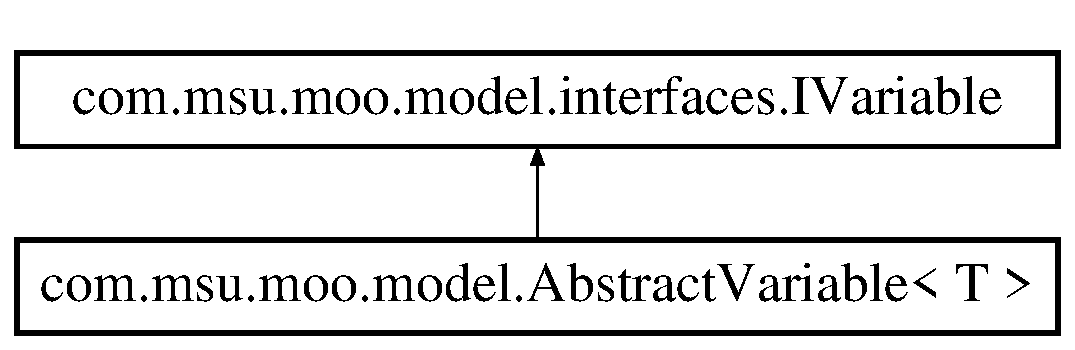
\includegraphics[height=2.000000cm]{interfacecom_1_1msu_1_1moo_1_1model_1_1interfaces_1_1IVariable}
\end{center}
\end{figure}
\subsection*{Public Member Functions}
\begin{DoxyCompactItemize}
\item 
Object \hyperlink{interfacecom_1_1msu_1_1moo_1_1model_1_1interfaces_1_1IVariable_a5d91fb013a9135144d975aa05b5f1b29}{get} ()
\item 
void \hyperlink{interfacecom_1_1msu_1_1moo_1_1model_1_1interfaces_1_1IVariable_a3bc30a747b2ee3c161fa3f6af8a9a061}{set} (Object obj)
\item 
\hyperlink{interfacecom_1_1msu_1_1moo_1_1model_1_1interfaces_1_1IVariable}{I\-Variable} \hyperlink{interfacecom_1_1msu_1_1moo_1_1model_1_1interfaces_1_1IVariable_aca748275c7293a63283ada1a665c6c28}{copy} ()
\end{DoxyCompactItemize}


\subsection{Detailed Description}
Interface for any variable that could be used. 

\subsection{Member Function Documentation}
\hypertarget{interfacecom_1_1msu_1_1moo_1_1model_1_1interfaces_1_1IVariable_aca748275c7293a63283ada1a665c6c28}{\index{com\-::msu\-::moo\-::model\-::interfaces\-::\-I\-Variable@{com\-::msu\-::moo\-::model\-::interfaces\-::\-I\-Variable}!copy@{copy}}
\index{copy@{copy}!com::msu::moo::model::interfaces::IVariable@{com\-::msu\-::moo\-::model\-::interfaces\-::\-I\-Variable}}
\subsubsection[{copy}]{\setlength{\rightskip}{0pt plus 5cm}{\bf I\-Variable} com.\-msu.\-moo.\-model.\-interfaces.\-I\-Variable.\-copy (
\begin{DoxyParamCaption}
{}
\end{DoxyParamCaption}
)}}\label{interfacecom_1_1msu_1_1moo_1_1model_1_1interfaces_1_1IVariable_aca748275c7293a63283ada1a665c6c28}
\begin{DoxyReturn}{Returns}
copy of the current variable 
\end{DoxyReturn}


Implemented in \hyperlink{classcom_1_1msu_1_1moo_1_1model_1_1AbstractVariable_3_01T_01_4_ab11df1a0613f42b0f1aed2226c666da2}{com.\-msu.\-moo.\-model.\-Abstract\-Variable$<$ T $>$}.

\hypertarget{interfacecom_1_1msu_1_1moo_1_1model_1_1interfaces_1_1IVariable_a5d91fb013a9135144d975aa05b5f1b29}{\index{com\-::msu\-::moo\-::model\-::interfaces\-::\-I\-Variable@{com\-::msu\-::moo\-::model\-::interfaces\-::\-I\-Variable}!get@{get}}
\index{get@{get}!com::msu::moo::model::interfaces::IVariable@{com\-::msu\-::moo\-::model\-::interfaces\-::\-I\-Variable}}
\subsubsection[{get}]{\setlength{\rightskip}{0pt plus 5cm}Object com.\-msu.\-moo.\-model.\-interfaces.\-I\-Variable.\-get (
\begin{DoxyParamCaption}
{}
\end{DoxyParamCaption}
)}}\label{interfacecom_1_1msu_1_1moo_1_1model_1_1interfaces_1_1IVariable_a5d91fb013a9135144d975aa05b5f1b29}
\begin{DoxyReturn}{Returns}
the variable by it self 
\end{DoxyReturn}


Implemented in \hyperlink{classcom_1_1msu_1_1moo_1_1model_1_1AbstractVariable_3_01T_01_4_a4c969f78e29f71436eb1f2db62fd43c5}{com.\-msu.\-moo.\-model.\-Abstract\-Variable$<$ T $>$}.

\hypertarget{interfacecom_1_1msu_1_1moo_1_1model_1_1interfaces_1_1IVariable_a3bc30a747b2ee3c161fa3f6af8a9a061}{\index{com\-::msu\-::moo\-::model\-::interfaces\-::\-I\-Variable@{com\-::msu\-::moo\-::model\-::interfaces\-::\-I\-Variable}!set@{set}}
\index{set@{set}!com::msu::moo::model::interfaces::IVariable@{com\-::msu\-::moo\-::model\-::interfaces\-::\-I\-Variable}}
\subsubsection[{set}]{\setlength{\rightskip}{0pt plus 5cm}void com.\-msu.\-moo.\-model.\-interfaces.\-I\-Variable.\-set (
\begin{DoxyParamCaption}
\item[{Object}]{obj}
\end{DoxyParamCaption}
)}}\label{interfacecom_1_1msu_1_1moo_1_1model_1_1interfaces_1_1IVariable_a3bc30a747b2ee3c161fa3f6af8a9a061}
Set the value for the variable 

Implemented in \hyperlink{classcom_1_1msu_1_1moo_1_1model_1_1AbstractVariable_3_01T_01_4_ad3b3dfcb1027411ca8adc0a2e82a42d2}{com.\-msu.\-moo.\-model.\-Abstract\-Variable$<$ T $>$}.



The documentation for this interface was generated from the following file\-:\begin{DoxyCompactItemize}
\item 
src/main/java/com/msu/moo/model/interfaces/I\-Variable.\-java\end{DoxyCompactItemize}

\hypertarget{classcom_1_1msu_1_1moo_1_1problems_1_1Kursawe}{\section{com.\-msu.\-moo.\-problems.\-Kursawe Class Reference}
\label{classcom_1_1msu_1_1moo_1_1problems_1_1Kursawe}\index{com.\-msu.\-moo.\-problems.\-Kursawe@{com.\-msu.\-moo.\-problems.\-Kursawe}}
}
Inheritance diagram for com.\-msu.\-moo.\-problems.\-Kursawe\-:\begin{figure}[H]
\begin{center}
\leavevmode
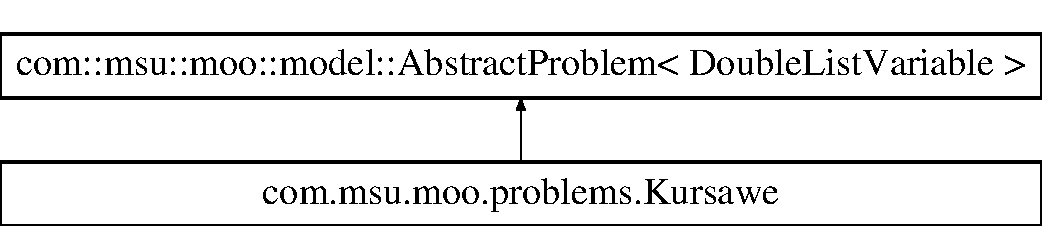
\includegraphics[height=2.000000cm]{classcom_1_1msu_1_1moo_1_1problems_1_1Kursawe}
\end{center}
\end{figure}
\subsection*{Public Member Functions}
\begin{DoxyCompactItemize}
\item 
\hypertarget{classcom_1_1msu_1_1moo_1_1problems_1_1Kursawe_a0ec3c4c0209e1d26179832f4a40a4f2f}{int {\bfseries get\-Number\-Of\-Objectives} ()}\label{classcom_1_1msu_1_1moo_1_1problems_1_1Kursawe_a0ec3c4c0209e1d26179832f4a40a4f2f}

\end{DoxyCompactItemize}
\subsection*{Protected Member Functions}
\begin{DoxyCompactItemize}
\item 
\hypertarget{classcom_1_1msu_1_1moo_1_1problems_1_1Kursawe_ae7fc8a190a7ce2ae30ef0c6c2689bc78}{List$<$ Double $>$ {\bfseries evaluate\-\_\-} (\hyperlink{classcom_1_1msu_1_1moo_1_1model_1_1variables_1_1DoubleListVariable}{Double\-List\-Variable} var)}\label{classcom_1_1msu_1_1moo_1_1problems_1_1Kursawe_ae7fc8a190a7ce2ae30ef0c6c2689bc78}

\end{DoxyCompactItemize}


The documentation for this class was generated from the following file\-:\begin{DoxyCompactItemize}
\item 
src/main/java/com/msu/moo/problems/Kursawe.\-java\end{DoxyCompactItemize}

\hypertarget{classcom_1_1msu_1_1moo_1_1experiment_1_1impl_1_1KursaweExperiment}{\section{com.\-msu.\-moo.\-experiment.\-impl.\-Kursawe\-Experiment Class Reference}
\label{classcom_1_1msu_1_1moo_1_1experiment_1_1impl_1_1KursaweExperiment}\index{com.\-msu.\-moo.\-experiment.\-impl.\-Kursawe\-Experiment@{com.\-msu.\-moo.\-experiment.\-impl.\-Kursawe\-Experiment}}
}
Inheritance diagram for com.\-msu.\-moo.\-experiment.\-impl.\-Kursawe\-Experiment\-:\begin{figure}[H]
\begin{center}
\leavevmode
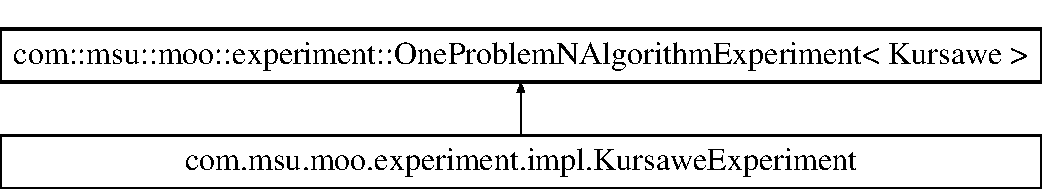
\includegraphics[height=2.000000cm]{classcom_1_1msu_1_1moo_1_1experiment_1_1impl_1_1KursaweExperiment}
\end{center}
\end{figure}
\subsection*{Static Public Member Functions}
\begin{DoxyCompactItemize}
\item 
\hypertarget{classcom_1_1msu_1_1moo_1_1experiment_1_1impl_1_1KursaweExperiment_a744c1633e78105230b74215066628c7b}{static void {\bfseries main} (String\mbox{[}$\,$\mbox{]} args)}\label{classcom_1_1msu_1_1moo_1_1experiment_1_1impl_1_1KursaweExperiment_a744c1633e78105230b74215066628c7b}

\end{DoxyCompactItemize}
\subsection*{Protected Member Functions}
\begin{DoxyCompactItemize}
\item 
\hypertarget{classcom_1_1msu_1_1moo_1_1experiment_1_1impl_1_1KursaweExperiment_a43e511805fc6818fcb914b5e61a7c9b4}{\hyperlink{classcom_1_1msu_1_1moo_1_1problems_1_1Kursawe}{Kursawe} {\bfseries get\-Problem} ()}\label{classcom_1_1msu_1_1moo_1_1experiment_1_1impl_1_1KursaweExperiment_a43e511805fc6818fcb914b5e61a7c9b4}

\item 
\hypertarget{classcom_1_1msu_1_1moo_1_1experiment_1_1impl_1_1KursaweExperiment_ae4f11e4be9bc76ecaf316ceb836b4cc4}{\hyperlink{classcom_1_1msu_1_1moo_1_1model_1_1solution_1_1NonDominatedSolutionSet}{Non\-Dominated\-Solution\-Set} {\bfseries get\-True\-Front} ()}\label{classcom_1_1msu_1_1moo_1_1experiment_1_1impl_1_1KursaweExperiment_ae4f11e4be9bc76ecaf316ceb836b4cc4}

\item 
\hypertarget{classcom_1_1msu_1_1moo_1_1experiment_1_1impl_1_1KursaweExperiment_a308ef56d8356092caf2a2fd96a0c709b}{List$<$ I\-Algorithm$<$ \hyperlink{classcom_1_1msu_1_1moo_1_1problems_1_1Kursawe}{Kursawe} $>$ $>$ {\bfseries get\-Algorithms} ()}\label{classcom_1_1msu_1_1moo_1_1experiment_1_1impl_1_1KursaweExperiment_a308ef56d8356092caf2a2fd96a0c709b}

\end{DoxyCompactItemize}


The documentation for this class was generated from the following file\-:\begin{DoxyCompactItemize}
\item 
src/main/java/com/msu/moo/experiment/impl/Kursawe\-Experiment.\-java\end{DoxyCompactItemize}

\hypertarget{classcom_1_1msu_1_1moo_1_1visualization_1_1LinePlot}{\section{com.\-msu.\-moo.\-visualization.\-Line\-Plot Class Reference}
\label{classcom_1_1msu_1_1moo_1_1visualization_1_1LinePlot}\index{com.\-msu.\-moo.\-visualization.\-Line\-Plot@{com.\-msu.\-moo.\-visualization.\-Line\-Plot}}
}
Inheritance diagram for com.\-msu.\-moo.\-visualization.\-Line\-Plot\-:\begin{figure}[H]
\begin{center}
\leavevmode
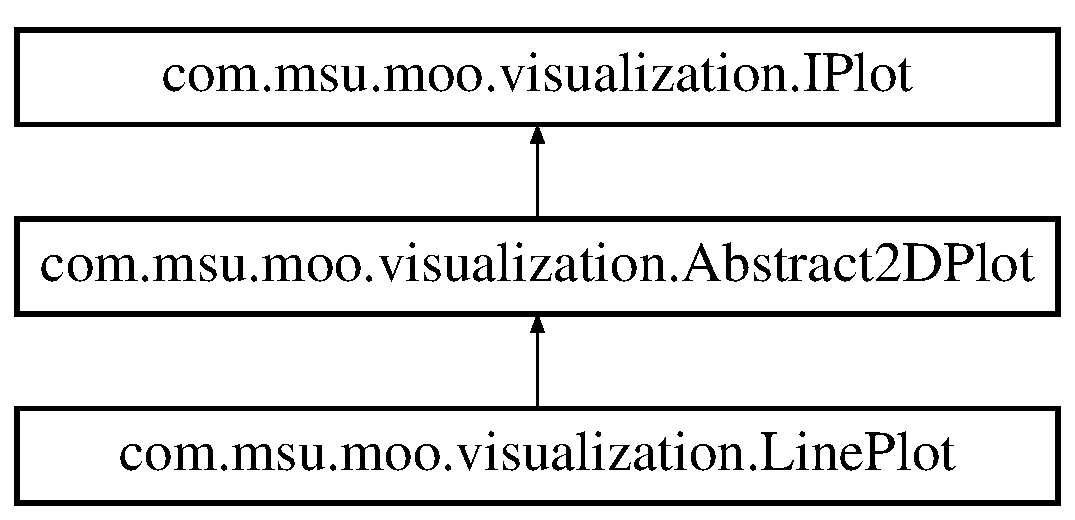
\includegraphics[height=3.000000cm]{classcom_1_1msu_1_1moo_1_1visualization_1_1LinePlot}
\end{center}
\end{figure}
\subsection*{Public Member Functions}
\begin{DoxyCompactItemize}
\item 
\hypertarget{classcom_1_1msu_1_1moo_1_1visualization_1_1LinePlot_a0942321b06078b0658d72150b94edb68}{{\bfseries Line\-Plot} (String title)}\label{classcom_1_1msu_1_1moo_1_1visualization_1_1LinePlot_a0942321b06078b0658d72150b94edb68}

\item 
\hypertarget{classcom_1_1msu_1_1moo_1_1visualization_1_1LinePlot_a15588aebe9683b1338de9b79b6d88caa}{void {\bfseries add} (List$<$ List$<$ Double $>$$>$ l, String name)}\label{classcom_1_1msu_1_1moo_1_1visualization_1_1LinePlot_a15588aebe9683b1338de9b79b6d88caa}

\item 
J\-Free\-Chart \hyperlink{classcom_1_1msu_1_1moo_1_1visualization_1_1LinePlot_ab6bc90e83277d08e59c3efd82e3b585d}{get\-Chart} ()
\end{DoxyCompactItemize}
\subsection*{Protected Attributes}
\begin{DoxyCompactItemize}
\item 
\hypertarget{classcom_1_1msu_1_1moo_1_1visualization_1_1LinePlot_ab718a71f3ea42c7811f8f25dd2b2fd3b}{X\-Y\-Series\-Collection {\bfseries set} = new X\-Y\-Series\-Collection()}\label{classcom_1_1msu_1_1moo_1_1visualization_1_1LinePlot_ab718a71f3ea42c7811f8f25dd2b2fd3b}

\end{DoxyCompactItemize}


\subsection{Member Function Documentation}
\hypertarget{classcom_1_1msu_1_1moo_1_1visualization_1_1LinePlot_ab6bc90e83277d08e59c3efd82e3b585d}{\index{com\-::msu\-::moo\-::visualization\-::\-Line\-Plot@{com\-::msu\-::moo\-::visualization\-::\-Line\-Plot}!get\-Chart@{get\-Chart}}
\index{get\-Chart@{get\-Chart}!com::msu::moo::visualization::LinePlot@{com\-::msu\-::moo\-::visualization\-::\-Line\-Plot}}
\subsubsection[{get\-Chart}]{\setlength{\rightskip}{0pt plus 5cm}J\-Free\-Chart com.\-msu.\-moo.\-visualization.\-Line\-Plot.\-get\-Chart (
\begin{DoxyParamCaption}
{}
\end{DoxyParamCaption}
)\hspace{0.3cm}{\ttfamily [inline]}}}\label{classcom_1_1msu_1_1moo_1_1visualization_1_1LinePlot_ab6bc90e83277d08e59c3efd82e3b585d}
Every Plot needs the chart frame to visualize the results \begin{DoxyReturn}{Returns}
chart frame to make it visible 
\end{DoxyReturn}


Implements \hyperlink{interfacecom_1_1msu_1_1moo_1_1visualization_1_1IPlot_ae45c2987d112fbf5bc5af7864fb50ecd}{com.\-msu.\-moo.\-visualization.\-I\-Plot}.



The documentation for this class was generated from the following file\-:\begin{DoxyCompactItemize}
\item 
src/main/java/com/msu/moo/visualization/Line\-Plot.\-java\end{DoxyCompactItemize}

\hypertarget{classcom_1_1msu_1_1moo_1_1model_1_1variables_1_1ListVariable_3_01T_01_4}{\section{com.\-msu.\-moo.\-model.\-variables.\-List\-Variable$<$ T $>$ Class Reference}
\label{classcom_1_1msu_1_1moo_1_1model_1_1variables_1_1ListVariable_3_01T_01_4}\index{com.\-msu.\-moo.\-model.\-variables.\-List\-Variable$<$ T $>$@{com.\-msu.\-moo.\-model.\-variables.\-List\-Variable$<$ T $>$}}
}
Inheritance diagram for com.\-msu.\-moo.\-model.\-variables.\-List\-Variable$<$ T $>$\-:\begin{figure}[H]
\begin{center}
\leavevmode
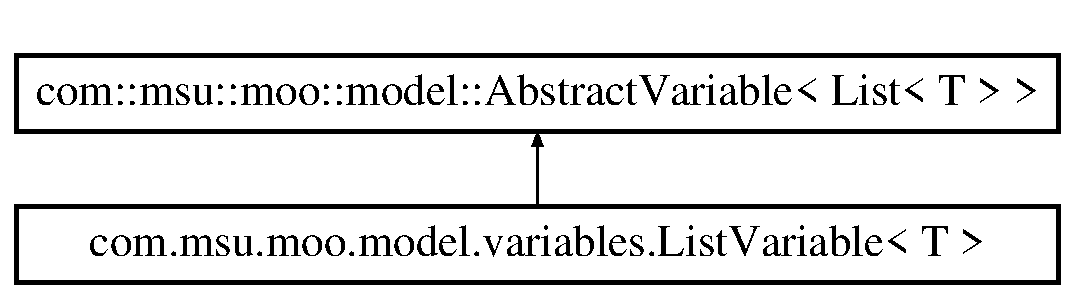
\includegraphics[height=2.000000cm]{classcom_1_1msu_1_1moo_1_1model_1_1variables_1_1ListVariable_3_01T_01_4}
\end{center}
\end{figure}
\subsection*{Public Member Functions}
\begin{DoxyCompactItemize}
\item 
\hypertarget{classcom_1_1msu_1_1moo_1_1model_1_1variables_1_1ListVariable_3_01T_01_4_ad428328d5633adb151e789e8eaa41781}{{\bfseries List\-Variable} (List$<$ T $>$ obj)}\label{classcom_1_1msu_1_1moo_1_1model_1_1variables_1_1ListVariable_3_01T_01_4_ad428328d5633adb151e789e8eaa41781}

\item 
\hypertarget{classcom_1_1msu_1_1moo_1_1model_1_1variables_1_1ListVariable_3_01T_01_4_a421be3d632446e271af32b99614d202b}{String {\bfseries to\-String} ()}\label{classcom_1_1msu_1_1moo_1_1model_1_1variables_1_1ListVariable_3_01T_01_4_a421be3d632446e271af32b99614d202b}

\item 
\hypertarget{classcom_1_1msu_1_1moo_1_1model_1_1variables_1_1ListVariable_3_01T_01_4_aaed85224a18f220ebafc07c112230ff6}{\hyperlink{interfacecom_1_1msu_1_1moo_1_1model_1_1interfaces_1_1IVariable}{I\-Variable} {\bfseries copy} ()}\label{classcom_1_1msu_1_1moo_1_1model_1_1variables_1_1ListVariable_3_01T_01_4_aaed85224a18f220ebafc07c112230ff6}

\end{DoxyCompactItemize}


The documentation for this class was generated from the following file\-:\begin{DoxyCompactItemize}
\item 
src/main/java/com/msu/moo/model/variables/List\-Variable.\-java\end{DoxyCompactItemize}

\hypertarget{classcom_1_1msu_1_1moo_1_1util_1_1sorting_1_1NaiveNonDominatedSorting}{\section{com.\-msu.\-moo.\-util.\-sorting.\-Naive\-Non\-Dominated\-Sorting Class Reference}
\label{classcom_1_1msu_1_1moo_1_1util_1_1sorting_1_1NaiveNonDominatedSorting}\index{com.\-msu.\-moo.\-util.\-sorting.\-Naive\-Non\-Dominated\-Sorting@{com.\-msu.\-moo.\-util.\-sorting.\-Naive\-Non\-Dominated\-Sorting}}
}
Inheritance diagram for com.\-msu.\-moo.\-util.\-sorting.\-Naive\-Non\-Dominated\-Sorting\-:\begin{figure}[H]
\begin{center}
\leavevmode
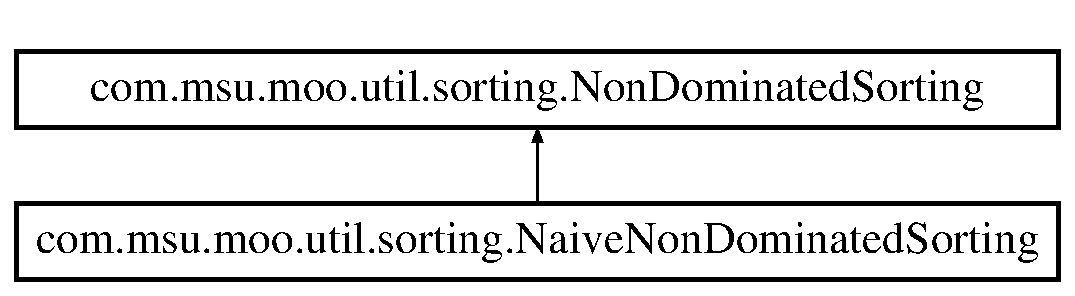
\includegraphics[height=2.000000cm]{classcom_1_1msu_1_1moo_1_1util_1_1sorting_1_1NaiveNonDominatedSorting}
\end{center}
\end{figure}
\subsection*{Public Member Functions}
\begin{DoxyCompactItemize}
\item 
\hypertarget{classcom_1_1msu_1_1moo_1_1util_1_1sorting_1_1NaiveNonDominatedSorting_a803cd43127e54f700b217ff02f1f396c}{List$<$ \hyperlink{classcom_1_1msu_1_1moo_1_1model_1_1solution_1_1NonDominatedSolutionSet}{Non\-Dominated\-Solution\-Set} $>$ {\bfseries run} (List$<$ \hyperlink{classcom_1_1msu_1_1moo_1_1model_1_1solution_1_1Solution}{Solution} $>$ solutions)}\label{classcom_1_1msu_1_1moo_1_1util_1_1sorting_1_1NaiveNonDominatedSorting_a803cd43127e54f700b217ff02f1f396c}

\end{DoxyCompactItemize}


\subsection{Detailed Description}
Implementation of a naive approach which searching for the current front off all individuals. Then the front is removed from the set and the step is repeated until there are no elements. 

The documentation for this class was generated from the following file\-:\begin{DoxyCompactItemize}
\item 
src/main/java/com/msu/moo/util/sorting/Naive\-Non\-Dominated\-Sorting.\-java\end{DoxyCompactItemize}

\hypertarget{classcom_1_1msu_1_1moo_1_1util_1_1indicator_1_1NonDominatedRankIndicator}{\section{com.\-msu.\-moo.\-util.\-indicator.\-Non\-Dominated\-Rank\-Indicator Class Reference}
\label{classcom_1_1msu_1_1moo_1_1util_1_1indicator_1_1NonDominatedRankIndicator}\index{com.\-msu.\-moo.\-util.\-indicator.\-Non\-Dominated\-Rank\-Indicator@{com.\-msu.\-moo.\-util.\-indicator.\-Non\-Dominated\-Rank\-Indicator}}
}
Inheritance diagram for com.\-msu.\-moo.\-util.\-indicator.\-Non\-Dominated\-Rank\-Indicator\-:\begin{figure}[H]
\begin{center}
\leavevmode
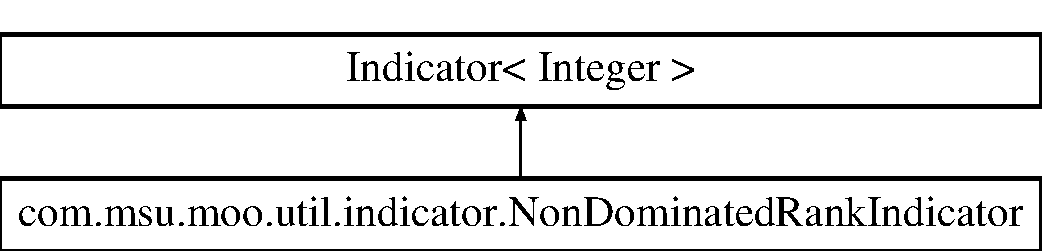
\includegraphics[height=2.000000cm]{classcom_1_1msu_1_1moo_1_1util_1_1indicator_1_1NonDominatedRankIndicator}
\end{center}
\end{figure}
\subsection*{Public Member Functions}
\begin{DoxyCompactItemize}
\item 
\hypertarget{classcom_1_1msu_1_1moo_1_1util_1_1indicator_1_1NonDominatedRankIndicator_a04eacae8ef154e5593e09c7555e1fbaf}{{\bfseries Non\-Dominated\-Rank\-Indicator} (\hyperlink{interfacecom_1_1msu_1_1moo_1_1util_1_1sorting_1_1NonDominatedSorting}{Non\-Dominated\-Sorting} sort)}\label{classcom_1_1msu_1_1moo_1_1util_1_1indicator_1_1NonDominatedRankIndicator_a04eacae8ef154e5593e09c7555e1fbaf}

\item 
\hypertarget{classcom_1_1msu_1_1moo_1_1util_1_1indicator_1_1NonDominatedRankIndicator_ac8b518291937a08166a49ddf378f4d25}{void {\bfseries calculate} (Map$<$ \hyperlink{classcom_1_1msu_1_1moo_1_1model_1_1solution_1_1Solution}{Solution}, Integer $>$ map, \hyperlink{classcom_1_1msu_1_1moo_1_1model_1_1solution_1_1SolutionSet}{Solution\-Set} solutions)}\label{classcom_1_1msu_1_1moo_1_1util_1_1indicator_1_1NonDominatedRankIndicator_ac8b518291937a08166a49ddf378f4d25}

\item 
List$<$ \hyperlink{classcom_1_1msu_1_1moo_1_1model_1_1solution_1_1NonDominatedSolutionSet}{Non\-Dominated\-Solution\-Set} $>$ \hyperlink{classcom_1_1msu_1_1moo_1_1util_1_1indicator_1_1NonDominatedRankIndicator_a01b03eefb37e8b671fb00ef0a605d340}{get\-Non\-Dominated\-Sets} ()
\end{DoxyCompactItemize}
\subsection*{Protected Attributes}
\begin{DoxyCompactItemize}
\item 
\hypertarget{classcom_1_1msu_1_1moo_1_1util_1_1indicator_1_1NonDominatedRankIndicator_af6ad2ed42de0ccdb8a9c13b54a9ff0a1}{\hyperlink{interfacecom_1_1msu_1_1moo_1_1util_1_1sorting_1_1NonDominatedSorting}{Non\-Dominated\-Sorting} {\bfseries sort} = new \hyperlink{classcom_1_1msu_1_1moo_1_1util_1_1sorting_1_1NaiveNonDominatedSorting}{Naive\-Non\-Dominated\-Sorting}()}\label{classcom_1_1msu_1_1moo_1_1util_1_1indicator_1_1NonDominatedRankIndicator_af6ad2ed42de0ccdb8a9c13b54a9ff0a1}

\item 
\hypertarget{classcom_1_1msu_1_1moo_1_1util_1_1indicator_1_1NonDominatedRankIndicator_abc1e889225e500ab0b5e3478b4521c32}{List$<$ \hyperlink{classcom_1_1msu_1_1moo_1_1model_1_1solution_1_1NonDominatedSolutionSet}{Non\-Dominated\-Solution\-Set} $>$ \hyperlink{classcom_1_1msu_1_1moo_1_1util_1_1indicator_1_1NonDominatedRankIndicator_abc1e889225e500ab0b5e3478b4521c32}{sets} = null}\label{classcom_1_1msu_1_1moo_1_1util_1_1indicator_1_1NonDominatedRankIndicator_abc1e889225e500ab0b5e3478b4521c32}

\begin{DoxyCompactList}\small\item\em when you have calculated the fronts you have access to the list of fronts. \end{DoxyCompactList}\end{DoxyCompactItemize}


\subsection{Member Function Documentation}
\hypertarget{classcom_1_1msu_1_1moo_1_1util_1_1indicator_1_1NonDominatedRankIndicator_a01b03eefb37e8b671fb00ef0a605d340}{\index{com\-::msu\-::moo\-::util\-::indicator\-::\-Non\-Dominated\-Rank\-Indicator@{com\-::msu\-::moo\-::util\-::indicator\-::\-Non\-Dominated\-Rank\-Indicator}!get\-Non\-Dominated\-Sets@{get\-Non\-Dominated\-Sets}}
\index{get\-Non\-Dominated\-Sets@{get\-Non\-Dominated\-Sets}!com::msu::moo::util::indicator::NonDominatedRankIndicator@{com\-::msu\-::moo\-::util\-::indicator\-::\-Non\-Dominated\-Rank\-Indicator}}
\subsubsection[{get\-Non\-Dominated\-Sets}]{\setlength{\rightskip}{0pt plus 5cm}List$<${\bf Non\-Dominated\-Solution\-Set}$>$ com.\-msu.\-moo.\-util.\-indicator.\-Non\-Dominated\-Rank\-Indicator.\-get\-Non\-Dominated\-Sets (
\begin{DoxyParamCaption}
{}
\end{DoxyParamCaption}
)\hspace{0.3cm}{\ttfamily [inline]}}}\label{classcom_1_1msu_1_1moo_1_1util_1_1indicator_1_1NonDominatedRankIndicator_a01b03eefb37e8b671fb00ef0a605d340}
\begin{DoxyReturn}{Returns}
all the fronts that were used to determine the rank of each solution 
\end{DoxyReturn}


The documentation for this class was generated from the following file\-:\begin{DoxyCompactItemize}
\item 
src/main/java/com/msu/moo/util/indicator/Non\-Dominated\-Rank\-Indicator.\-java\end{DoxyCompactItemize}

\hypertarget{classcom_1_1msu_1_1moo_1_1model_1_1solution_1_1NonDominatedSolutionSet}{\section{com.\-msu.\-moo.\-model.\-solution.\-Non\-Dominated\-Solution\-Set Class Reference}
\label{classcom_1_1msu_1_1moo_1_1model_1_1solution_1_1NonDominatedSolutionSet}\index{com.\-msu.\-moo.\-model.\-solution.\-Non\-Dominated\-Solution\-Set@{com.\-msu.\-moo.\-model.\-solution.\-Non\-Dominated\-Solution\-Set}}
}
\subsection*{Public Member Functions}
\begin{DoxyCompactItemize}
\item 
\hypertarget{classcom_1_1msu_1_1moo_1_1model_1_1solution_1_1NonDominatedSolutionSet_a4c3b6cdd3d13eec16962105474d4b6ca}{{\bfseries Non\-Dominated\-Solution\-Set} (\hyperlink{classcom_1_1msu_1_1moo_1_1model_1_1solution_1_1NonDominatedSolutionSet}{Non\-Dominated\-Solution\-Set} set)}\label{classcom_1_1msu_1_1moo_1_1model_1_1solution_1_1NonDominatedSolutionSet_a4c3b6cdd3d13eec16962105474d4b6ca}

\item 
\hypertarget{classcom_1_1msu_1_1moo_1_1model_1_1solution_1_1NonDominatedSolutionSet_a1a9f64544c83cff6b7caab2de1689505}{{\bfseries Non\-Dominated\-Solution\-Set} (List$<$ \hyperlink{classcom_1_1msu_1_1moo_1_1model_1_1solution_1_1Solution}{Solution} $>$ \hyperlink{classcom_1_1msu_1_1moo_1_1model_1_1solution_1_1NonDominatedSolutionSet_a9c1ad52b072eabc7faff33b81f86c4d4}{solutions})}\label{classcom_1_1msu_1_1moo_1_1model_1_1solution_1_1NonDominatedSolutionSet_a1a9f64544c83cff6b7caab2de1689505}

\item 
\hypertarget{classcom_1_1msu_1_1moo_1_1model_1_1solution_1_1NonDominatedSolutionSet_a3658a7572377ba1ba0055e01de918034}{boolean {\bfseries add} (\hyperlink{classcom_1_1msu_1_1moo_1_1model_1_1solution_1_1Solution}{Solution} solution\-To\-Add)}\label{classcom_1_1msu_1_1moo_1_1model_1_1solution_1_1NonDominatedSolutionSet_a3658a7572377ba1ba0055e01de918034}

\item 
int \hyperlink{classcom_1_1msu_1_1moo_1_1model_1_1solution_1_1NonDominatedSolutionSet_a8a408462f28e01a2f32c292daeb68ac9}{size} ()
\item 
\hyperlink{classcom_1_1msu_1_1moo_1_1model_1_1solution_1_1SolutionSet}{Solution\-Set} \hyperlink{classcom_1_1msu_1_1moo_1_1model_1_1solution_1_1NonDominatedSolutionSet_a1fcaff0392af7b98d4dc6c9016829a49}{get\-Solutions} ()
\item 
\hypertarget{classcom_1_1msu_1_1moo_1_1model_1_1solution_1_1NonDominatedSolutionSet_a914b87fe2969b3d7f24f7bf018b5ee9f}{String {\bfseries to\-String} ()}\label{classcom_1_1msu_1_1moo_1_1model_1_1solution_1_1NonDominatedSolutionSet_a914b87fe2969b3d7f24f7bf018b5ee9f}

\item 
\hypertarget{classcom_1_1msu_1_1moo_1_1model_1_1solution_1_1NonDominatedSolutionSet_add2bfeb7adec377a5b335fb640fa9752}{Range$<$ Double $>$ {\bfseries get\-Range} ()}\label{classcom_1_1msu_1_1moo_1_1model_1_1solution_1_1NonDominatedSolutionSet_add2bfeb7adec377a5b335fb640fa9752}

\end{DoxyCompactItemize}
\subsection*{Protected Attributes}
\begin{DoxyCompactItemize}
\item 
\hypertarget{classcom_1_1msu_1_1moo_1_1model_1_1solution_1_1NonDominatedSolutionSet_a9c1ad52b072eabc7faff33b81f86c4d4}{\hyperlink{classcom_1_1msu_1_1moo_1_1model_1_1solution_1_1SolutionSet}{Solution\-Set} \hyperlink{classcom_1_1msu_1_1moo_1_1model_1_1solution_1_1NonDominatedSolutionSet_a9c1ad52b072eabc7faff33b81f86c4d4}{solutions} = new \hyperlink{classcom_1_1msu_1_1moo_1_1model_1_1solution_1_1SolutionSet}{Solution\-Set}()}\label{classcom_1_1msu_1_1moo_1_1model_1_1solution_1_1NonDominatedSolutionSet_a9c1ad52b072eabc7faff33b81f86c4d4}

\begin{DoxyCompactList}\small\item\em list which contains all the solutions \end{DoxyCompactList}\item 
\hypertarget{classcom_1_1msu_1_1moo_1_1model_1_1solution_1_1NonDominatedSolutionSet_a8cb3e256571393ce5d6b3226e8b2be6b}{\hyperlink{classcom_1_1msu_1_1moo_1_1model_1_1solution_1_1SolutionDominator}{Solution\-Dominator} \hyperlink{classcom_1_1msu_1_1moo_1_1model_1_1solution_1_1NonDominatedSolutionSet_a8cb3e256571393ce5d6b3226e8b2be6b}{cmp} = new \hyperlink{classcom_1_1msu_1_1moo_1_1model_1_1solution_1_1SolutionDominator}{Solution\-Dominator}()}\label{classcom_1_1msu_1_1moo_1_1model_1_1solution_1_1NonDominatedSolutionSet_a8cb3e256571393ce5d6b3226e8b2be6b}

\begin{DoxyCompactList}\small\item\em solution comparator for testing domination \end{DoxyCompactList}\end{DoxyCompactItemize}


\subsection{Member Function Documentation}
\hypertarget{classcom_1_1msu_1_1moo_1_1model_1_1solution_1_1NonDominatedSolutionSet_a1fcaff0392af7b98d4dc6c9016829a49}{\index{com\-::msu\-::moo\-::model\-::solution\-::\-Non\-Dominated\-Solution\-Set@{com\-::msu\-::moo\-::model\-::solution\-::\-Non\-Dominated\-Solution\-Set}!get\-Solutions@{get\-Solutions}}
\index{get\-Solutions@{get\-Solutions}!com::msu::moo::model::solution::NonDominatedSolutionSet@{com\-::msu\-::moo\-::model\-::solution\-::\-Non\-Dominated\-Solution\-Set}}
\subsubsection[{get\-Solutions}]{\setlength{\rightskip}{0pt plus 5cm}{\bf Solution\-Set} com.\-msu.\-moo.\-model.\-solution.\-Non\-Dominated\-Solution\-Set.\-get\-Solutions (
\begin{DoxyParamCaption}
{}
\end{DoxyParamCaption}
)\hspace{0.3cm}{\ttfamily [inline]}}}\label{classcom_1_1msu_1_1moo_1_1model_1_1solution_1_1NonDominatedSolutionSet_a1fcaff0392af7b98d4dc6c9016829a49}
\begin{DoxyReturn}{Returns}
all the solutions in a list! 
\end{DoxyReturn}
\hypertarget{classcom_1_1msu_1_1moo_1_1model_1_1solution_1_1NonDominatedSolutionSet_a8a408462f28e01a2f32c292daeb68ac9}{\index{com\-::msu\-::moo\-::model\-::solution\-::\-Non\-Dominated\-Solution\-Set@{com\-::msu\-::moo\-::model\-::solution\-::\-Non\-Dominated\-Solution\-Set}!size@{size}}
\index{size@{size}!com::msu::moo::model::solution::NonDominatedSolutionSet@{com\-::msu\-::moo\-::model\-::solution\-::\-Non\-Dominated\-Solution\-Set}}
\subsubsection[{size}]{\setlength{\rightskip}{0pt plus 5cm}int com.\-msu.\-moo.\-model.\-solution.\-Non\-Dominated\-Solution\-Set.\-size (
\begin{DoxyParamCaption}
{}
\end{DoxyParamCaption}
)\hspace{0.3cm}{\ttfamily [inline]}}}\label{classcom_1_1msu_1_1moo_1_1model_1_1solution_1_1NonDominatedSolutionSet_a8a408462f28e01a2f32c292daeb68ac9}
\begin{DoxyReturn}{Returns}
the current size of the set. 
\end{DoxyReturn}


The documentation for this class was generated from the following file\-:\begin{DoxyCompactItemize}
\item 
src/main/java/com/msu/moo/model/solution/Non\-Dominated\-Solution\-Set.\-java\end{DoxyCompactItemize}

\hypertarget{interfacecom_1_1msu_1_1moo_1_1util_1_1sorting_1_1NonDominatedSorting}{\section{com.\-msu.\-moo.\-util.\-sorting.\-Non\-Dominated\-Sorting Interface Reference}
\label{interfacecom_1_1msu_1_1moo_1_1util_1_1sorting_1_1NonDominatedSorting}\index{com.\-msu.\-moo.\-util.\-sorting.\-Non\-Dominated\-Sorting@{com.\-msu.\-moo.\-util.\-sorting.\-Non\-Dominated\-Sorting}}
}
Inheritance diagram for com.\-msu.\-moo.\-util.\-sorting.\-Non\-Dominated\-Sorting\-:\begin{figure}[H]
\begin{center}
\leavevmode
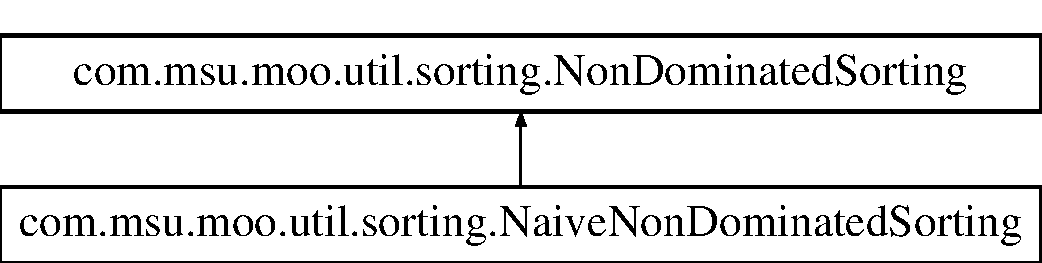
\includegraphics[height=2.000000cm]{interfacecom_1_1msu_1_1moo_1_1util_1_1sorting_1_1NonDominatedSorting}
\end{center}
\end{figure}
\subsection*{Public Member Functions}
\begin{DoxyCompactItemize}
\item 
\hypertarget{interfacecom_1_1msu_1_1moo_1_1util_1_1sorting_1_1NonDominatedSorting_a0d6a8e9261e231598a4f8aa45970bd5a}{List$<$ \hyperlink{classcom_1_1msu_1_1moo_1_1model_1_1solution_1_1NonDominatedSolutionSet}{Non\-Dominated\-Solution\-Set} $>$ {\bfseries run} (List$<$ \hyperlink{classcom_1_1msu_1_1moo_1_1model_1_1solution_1_1Solution}{Solution} $>$ solutions)}\label{interfacecom_1_1msu_1_1moo_1_1util_1_1sorting_1_1NonDominatedSorting_a0d6a8e9261e231598a4f8aa45970bd5a}

\end{DoxyCompactItemize}


\subsection{Detailed Description}
This interface provides general sorting approach which means to get the different fronts of many solutions. 

The documentation for this interface was generated from the following file\-:\begin{DoxyCompactItemize}
\item 
src/main/java/com/msu/moo/util/sorting/Non\-Dominated\-Sorting.\-java\end{DoxyCompactItemize}

\hypertarget{classcom_1_1msu_1_1moo_1_1operators_1_1crossover_1_1NPointCrossover_3_01T_01_4}{\section{com.\-msu.\-moo.\-operators.\-crossover.\-N\-Point\-Crossover$<$ T $>$ Class Reference}
\label{classcom_1_1msu_1_1moo_1_1operators_1_1crossover_1_1NPointCrossover_3_01T_01_4}\index{com.\-msu.\-moo.\-operators.\-crossover.\-N\-Point\-Crossover$<$ T $>$@{com.\-msu.\-moo.\-operators.\-crossover.\-N\-Point\-Crossover$<$ T $>$}}
}
Inheritance diagram for com.\-msu.\-moo.\-operators.\-crossover.\-N\-Point\-Crossover$<$ T $>$\-:\begin{figure}[H]
\begin{center}
\leavevmode
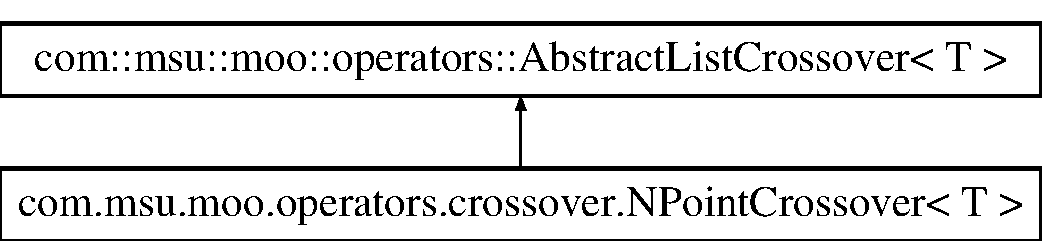
\includegraphics[height=2.000000cm]{classcom_1_1msu_1_1moo_1_1operators_1_1crossover_1_1NPointCrossover_3_01T_01_4}
\end{center}
\end{figure}
\subsection*{Public Member Functions}
\begin{DoxyCompactItemize}
\item 
\hypertarget{classcom_1_1msu_1_1moo_1_1operators_1_1crossover_1_1NPointCrossover_3_01T_01_4_a0843f9c0c4c1771aa6e7a87fba6b65d5}{{\bfseries N\-Point\-Crossover} (int crossover\-Points)}\label{classcom_1_1msu_1_1moo_1_1operators_1_1crossover_1_1NPointCrossover_3_01T_01_4_a0843f9c0c4c1771aa6e7a87fba6b65d5}

\end{DoxyCompactItemize}
\subsection*{Protected Member Functions}
\begin{DoxyCompactItemize}
\item 
\hypertarget{classcom_1_1msu_1_1moo_1_1operators_1_1crossover_1_1NPointCrossover_3_01T_01_4_abc6162ab69e933f36ce4cd06b3d5fbbe}{List$<$ List$<$ T $>$ $>$ {\bfseries crossover\-Lists} (List$<$ T $>$ p1, List$<$ T $>$ p2)}\label{classcom_1_1msu_1_1moo_1_1operators_1_1crossover_1_1NPointCrossover_3_01T_01_4_abc6162ab69e933f36ce4cd06b3d5fbbe}

\end{DoxyCompactItemize}
\subsection*{Protected Attributes}
\begin{DoxyCompactItemize}
\item 
\hypertarget{classcom_1_1msu_1_1moo_1_1operators_1_1crossover_1_1NPointCrossover_3_01T_01_4_a39425dd875d76ad48be0b3af8f50f0a2}{int {\bfseries crossover\-Points} = 2}\label{classcom_1_1msu_1_1moo_1_1operators_1_1crossover_1_1NPointCrossover_3_01T_01_4_a39425dd875d76ad48be0b3af8f50f0a2}

\end{DoxyCompactItemize}


The documentation for this class was generated from the following file\-:\begin{DoxyCompactItemize}
\item 
src/main/java/com/msu/moo/operators/crossover/N\-Point\-Crossover.\-java\end{DoxyCompactItemize}

\hypertarget{classcom_1_1msu_1_1moo_1_1experiment_1_1NProblemNAlgorithmExperiment_3_01P_01extends_01IProblem_01_4}{\section{com.\-msu.\-moo.\-experiment.\-N\-Problem\-N\-Algorithm\-Experiment$<$ P extends I\-Problem $>$ Class Reference}
\label{classcom_1_1msu_1_1moo_1_1experiment_1_1NProblemNAlgorithmExperiment_3_01P_01extends_01IProblem_01_4}\index{com.\-msu.\-moo.\-experiment.\-N\-Problem\-N\-Algorithm\-Experiment$<$ P extends I\-Problem $>$@{com.\-msu.\-moo.\-experiment.\-N\-Problem\-N\-Algorithm\-Experiment$<$ P extends I\-Problem $>$}}
}
Inheritance diagram for com.\-msu.\-moo.\-experiment.\-N\-Problem\-N\-Algorithm\-Experiment$<$ P extends I\-Problem $>$\-:\begin{figure}[H]
\begin{center}
\leavevmode
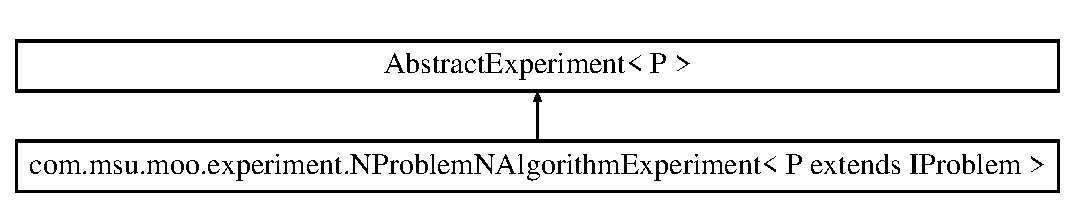
\includegraphics[height=2.000000cm]{classcom_1_1msu_1_1moo_1_1experiment_1_1NProblemNAlgorithmExperiment_3_01P_01extends_01IProblem_01_4}
\end{center}
\end{figure}
\subsection*{Public Member Functions}
\begin{DoxyCompactItemize}
\item 
\hypertarget{classcom_1_1msu_1_1moo_1_1experiment_1_1NProblemNAlgorithmExperiment_3_01P_01extends_01IProblem_01_4_ad241c0877d63849163f7a66c5723bc29}{void {\bfseries report} ()}\label{classcom_1_1msu_1_1moo_1_1experiment_1_1NProblemNAlgorithmExperiment_3_01P_01extends_01IProblem_01_4_ad241c0877d63849163f7a66c5723bc29}

\end{DoxyCompactItemize}
\subsection*{Protected Member Functions}
\begin{DoxyCompactItemize}
\item 
\hypertarget{classcom_1_1msu_1_1moo_1_1experiment_1_1NProblemNAlgorithmExperiment_3_01P_01extends_01IProblem_01_4_ababd618896299060ebe776f1c6249bb2}{void {\bfseries visualize} (P problem)}\label{classcom_1_1msu_1_1moo_1_1experiment_1_1NProblemNAlgorithmExperiment_3_01P_01extends_01IProblem_01_4_ababd618896299060ebe776f1c6249bb2}

\end{DoxyCompactItemize}


The documentation for this class was generated from the following file\-:\begin{DoxyCompactItemize}
\item 
src/main/java/com/msu/moo/experiment/N\-Problem\-N\-Algorithm\-Experiment.\-java\end{DoxyCompactItemize}

\hypertarget{classcom_1_1msu_1_1moo_1_1algorithms_1_1NSGAII_3_01V_01extends_01IVariable_00_01P_01extends_01IProblem_01_4}{\section{com.\-msu.\-moo.\-algorithms.\-N\-S\-G\-A\-I\-I$<$ V extends I\-Variable, P extends I\-Problem $>$ Class Reference}
\label{classcom_1_1msu_1_1moo_1_1algorithms_1_1NSGAII_3_01V_01extends_01IVariable_00_01P_01extends_01IProblem_01_4}\index{com.\-msu.\-moo.\-algorithms.\-N\-S\-G\-A\-I\-I$<$ V extends I\-Variable, P extends I\-Problem $>$@{com.\-msu.\-moo.\-algorithms.\-N\-S\-G\-A\-I\-I$<$ V extends I\-Variable, P extends I\-Problem $>$}}
}
Inheritance diagram for com.\-msu.\-moo.\-algorithms.\-N\-S\-G\-A\-I\-I$<$ V extends I\-Variable, P extends I\-Problem $>$\-:\begin{figure}[H]
\begin{center}
\leavevmode
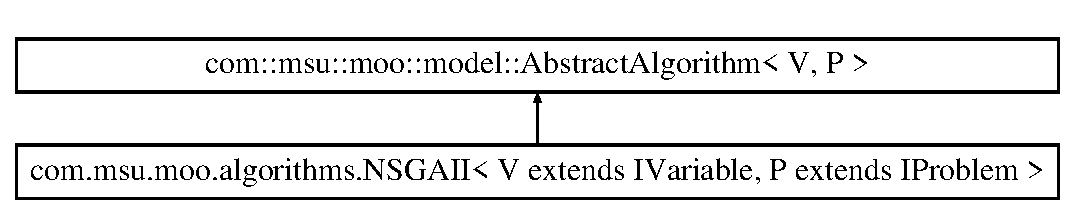
\includegraphics[height=2.000000cm]{classcom_1_1msu_1_1moo_1_1algorithms_1_1NSGAII_3_01V_01extends_01IVariable_00_01P_01extends_01IProblem_01_4}
\end{center}
\end{figure}
\subsection*{Public Member Functions}
\begin{DoxyCompactItemize}
\item 
\hypertarget{classcom_1_1msu_1_1moo_1_1algorithms_1_1NSGAII_3_01V_01extends_01IVariable_00_01P_01extends_01IProblem_01_4_abb6445eb2cb93423bbce94a33d18ef50}{{\bfseries N\-S\-G\-A\-I\-I} (Variable\-Factory$<$ V, P $>$ factory, Abstract\-Crossover$<$?$>$ \hyperlink{classcom_1_1msu_1_1moo_1_1algorithms_1_1NSGAII_3_01V_01extends_01IVariable_00_01P_01extends_01IProblem_01_4_a6f26592bf8c09db4e9eff203d6b830a1}{crossover}, Abstract\-Mutation$<$?$>$ \hyperlink{classcom_1_1msu_1_1moo_1_1algorithms_1_1NSGAII_3_01V_01extends_01IVariable_00_01P_01extends_01IProblem_01_4_a21edd4d5e0bf3a168b5f04f4df835ada}{mutation})}\label{classcom_1_1msu_1_1moo_1_1algorithms_1_1NSGAII_3_01V_01extends_01IVariable_00_01P_01extends_01IProblem_01_4_abb6445eb2cb93423bbce94a33d18ef50}

\item 
\hypertarget{classcom_1_1msu_1_1moo_1_1algorithms_1_1NSGAII_3_01V_01extends_01IVariable_00_01P_01extends_01IProblem_01_4_a0777d25d343c7c9ec24ca1516d29dcc4}{int {\bfseries get\-Population\-Size} ()}\label{classcom_1_1msu_1_1moo_1_1algorithms_1_1NSGAII_3_01V_01extends_01IVariable_00_01P_01extends_01IProblem_01_4_a0777d25d343c7c9ec24ca1516d29dcc4}

\item 
\hypertarget{classcom_1_1msu_1_1moo_1_1algorithms_1_1NSGAII_3_01V_01extends_01IVariable_00_01P_01extends_01IProblem_01_4_a6cfd4aa4c9d14954ef955a7cbb49096f}{void {\bfseries set\-Population\-Size} (int population\-Size)}\label{classcom_1_1msu_1_1moo_1_1algorithms_1_1NSGAII_3_01V_01extends_01IVariable_00_01P_01extends_01IProblem_01_4_a6cfd4aa4c9d14954ef955a7cbb49096f}

\end{DoxyCompactItemize}
\subsection*{Protected Member Functions}
\begin{DoxyCompactItemize}
\item 
\hypertarget{classcom_1_1msu_1_1moo_1_1algorithms_1_1NSGAII_3_01V_01extends_01IVariable_00_01P_01extends_01IProblem_01_4_a5c4e04a433a37a183801fe91ec2a9b52}{void {\bfseries calc\-Rank\-And\-Crowding} (\hyperlink{classcom_1_1msu_1_1moo_1_1model_1_1solution_1_1SolutionSet}{Solution\-Set} \hyperlink{classcom_1_1msu_1_1moo_1_1algorithms_1_1NSGAII_3_01V_01extends_01IVariable_00_01P_01extends_01IProblem_01_4_aa6f2611d1375c281a24bb08209eb6278}{population})}\label{classcom_1_1msu_1_1moo_1_1algorithms_1_1NSGAII_3_01V_01extends_01IVariable_00_01P_01extends_01IProblem_01_4_a5c4e04a433a37a183801fe91ec2a9b52}

\item 
\hypertarget{classcom_1_1msu_1_1moo_1_1algorithms_1_1NSGAII_3_01V_01extends_01IVariable_00_01P_01extends_01IProblem_01_4_ae4cfae255816510fd289f20018f6431d}{void {\bfseries initialize} ()}\label{classcom_1_1msu_1_1moo_1_1algorithms_1_1NSGAII_3_01V_01extends_01IVariable_00_01P_01extends_01IProblem_01_4_ae4cfae255816510fd289f20018f6431d}

\item 
\hypertarget{classcom_1_1msu_1_1moo_1_1algorithms_1_1NSGAII_3_01V_01extends_01IVariable_00_01P_01extends_01IProblem_01_4_ab87975ec6d7a2e07ff1f84fcf37baadd}{void {\bfseries next} ()}\label{classcom_1_1msu_1_1moo_1_1algorithms_1_1NSGAII_3_01V_01extends_01IVariable_00_01P_01extends_01IProblem_01_4_ab87975ec6d7a2e07ff1f84fcf37baadd}

\item 
\hypertarget{classcom_1_1msu_1_1moo_1_1algorithms_1_1NSGAII_3_01V_01extends_01IVariable_00_01P_01extends_01IProblem_01_4_a0c79bccef8bc08f93cda2e7a53edb97b}{\hyperlink{classcom_1_1msu_1_1moo_1_1model_1_1solution_1_1NonDominatedSolutionSet}{Non\-Dominated\-Solution\-Set} {\bfseries get\-Result} ()}\label{classcom_1_1msu_1_1moo_1_1algorithms_1_1NSGAII_3_01V_01extends_01IVariable_00_01P_01extends_01IProblem_01_4_a0c79bccef8bc08f93cda2e7a53edb97b}

\end{DoxyCompactItemize}
\subsection*{Protected Attributes}
\begin{DoxyCompactItemize}
\item 
\hypertarget{classcom_1_1msu_1_1moo_1_1algorithms_1_1NSGAII_3_01V_01extends_01IVariable_00_01P_01extends_01IProblem_01_4_a65cb1e4323f9be7c05e07088035f30eb}{int {\bfseries population\-Size} = 100}\label{classcom_1_1msu_1_1moo_1_1algorithms_1_1NSGAII_3_01V_01extends_01IVariable_00_01P_01extends_01IProblem_01_4_a65cb1e4323f9be7c05e07088035f30eb}

\item 
\hypertarget{classcom_1_1msu_1_1moo_1_1algorithms_1_1NSGAII_3_01V_01extends_01IVariable_00_01P_01extends_01IProblem_01_4_a671f3ed9e85a48eefba8ad74857120e3}{double \hyperlink{classcom_1_1msu_1_1moo_1_1algorithms_1_1NSGAII_3_01V_01extends_01IVariable_00_01P_01extends_01IProblem_01_4_a671f3ed9e85a48eefba8ad74857120e3}{prob\-Mutation} = 0.\-3}\label{classcom_1_1msu_1_1moo_1_1algorithms_1_1NSGAII_3_01V_01extends_01IVariable_00_01P_01extends_01IProblem_01_4_a671f3ed9e85a48eefba8ad74857120e3}

\begin{DoxyCompactList}\small\item\em default mutation probability \end{DoxyCompactList}\item 
\hypertarget{classcom_1_1msu_1_1moo_1_1algorithms_1_1NSGAII_3_01V_01extends_01IVariable_00_01P_01extends_01IProblem_01_4_a6f26592bf8c09db4e9eff203d6b830a1}{Abstract\-Crossover$<$?$>$ \hyperlink{classcom_1_1msu_1_1moo_1_1algorithms_1_1NSGAII_3_01V_01extends_01IVariable_00_01P_01extends_01IProblem_01_4_a6f26592bf8c09db4e9eff203d6b830a1}{crossover}}\label{classcom_1_1msu_1_1moo_1_1algorithms_1_1NSGAII_3_01V_01extends_01IVariable_00_01P_01extends_01IProblem_01_4_a6f26592bf8c09db4e9eff203d6b830a1}

\begin{DoxyCompactList}\small\item\em operator for crossover \end{DoxyCompactList}\item 
\hypertarget{classcom_1_1msu_1_1moo_1_1algorithms_1_1NSGAII_3_01V_01extends_01IVariable_00_01P_01extends_01IProblem_01_4_a21edd4d5e0bf3a168b5f04f4df835ada}{Abstract\-Mutation$<$?$>$ \hyperlink{classcom_1_1msu_1_1moo_1_1algorithms_1_1NSGAII_3_01V_01extends_01IVariable_00_01P_01extends_01IProblem_01_4_a21edd4d5e0bf3a168b5f04f4df835ada}{mutation}}\label{classcom_1_1msu_1_1moo_1_1algorithms_1_1NSGAII_3_01V_01extends_01IVariable_00_01P_01extends_01IProblem_01_4_a21edd4d5e0bf3a168b5f04f4df835ada}

\begin{DoxyCompactList}\small\item\em operator for mutation \end{DoxyCompactList}\item 
\hypertarget{classcom_1_1msu_1_1moo_1_1algorithms_1_1NSGAII_3_01V_01extends_01IVariable_00_01P_01extends_01IProblem_01_4_aa6f2611d1375c281a24bb08209eb6278}{\hyperlink{classcom_1_1msu_1_1moo_1_1model_1_1solution_1_1SolutionSet}{Solution\-Set} \hyperlink{classcom_1_1msu_1_1moo_1_1algorithms_1_1NSGAII_3_01V_01extends_01IVariable_00_01P_01extends_01IProblem_01_4_aa6f2611d1375c281a24bb08209eb6278}{population} = null}\label{classcom_1_1msu_1_1moo_1_1algorithms_1_1NSGAII_3_01V_01extends_01IVariable_00_01P_01extends_01IProblem_01_4_aa6f2611d1375c281a24bb08209eb6278}

\begin{DoxyCompactList}\small\item\em current population \end{DoxyCompactList}\item 
\hypertarget{classcom_1_1msu_1_1moo_1_1algorithms_1_1NSGAII_3_01V_01extends_01IVariable_00_01P_01extends_01IProblem_01_4_a295cd89e2476d609147aeecc77118d34}{Map$<$ \hyperlink{classcom_1_1msu_1_1moo_1_1model_1_1solution_1_1Solution}{Solution}, Integer $>$ \hyperlink{classcom_1_1msu_1_1moo_1_1algorithms_1_1NSGAII_3_01V_01extends_01IVariable_00_01P_01extends_01IProblem_01_4_a295cd89e2476d609147aeecc77118d34}{rank}}\label{classcom_1_1msu_1_1moo_1_1algorithms_1_1NSGAII_3_01V_01extends_01IVariable_00_01P_01extends_01IProblem_01_4_a295cd89e2476d609147aeecc77118d34}

\begin{DoxyCompactList}\small\item\em rank for the whole population \end{DoxyCompactList}\item 
\hypertarget{classcom_1_1msu_1_1moo_1_1algorithms_1_1NSGAII_3_01V_01extends_01IVariable_00_01P_01extends_01IProblem_01_4_a79a5b6f90573b528c174f1d91828a2ff}{Map$<$ \hyperlink{classcom_1_1msu_1_1moo_1_1model_1_1solution_1_1Solution}{Solution}, Double $>$ \hyperlink{classcom_1_1msu_1_1moo_1_1algorithms_1_1NSGAII_3_01V_01extends_01IVariable_00_01P_01extends_01IProblem_01_4_a79a5b6f90573b528c174f1d91828a2ff}{crowding}}\label{classcom_1_1msu_1_1moo_1_1algorithms_1_1NSGAII_3_01V_01extends_01IVariable_00_01P_01extends_01IProblem_01_4_a79a5b6f90573b528c174f1d91828a2ff}

\begin{DoxyCompactList}\small\item\em crowding distance for the whole population \end{DoxyCompactList}\end{DoxyCompactItemize}


The documentation for this class was generated from the following file\-:\begin{DoxyCompactItemize}
\item 
src/main/java/com/msu/moo/algorithms/N\-S\-G\-A\-I\-I.\-java\end{DoxyCompactItemize}

\hypertarget{classcom_1_1msu_1_1moo_1_1algorithms_1_1NSGAIIBuilder_3_01V_01extends_01IVariable_00_01P_01extends_01IProblem_01_4}{\section{com.\-msu.\-moo.\-algorithms.\-N\-S\-G\-A\-I\-I\-Builder$<$ V extends I\-Variable, P extends I\-Problem $>$ Class Reference}
\label{classcom_1_1msu_1_1moo_1_1algorithms_1_1NSGAIIBuilder_3_01V_01extends_01IVariable_00_01P_01extends_01IProblem_01_4}\index{com.\-msu.\-moo.\-algorithms.\-N\-S\-G\-A\-I\-I\-Builder$<$ V extends I\-Variable, P extends I\-Problem $>$@{com.\-msu.\-moo.\-algorithms.\-N\-S\-G\-A\-I\-I\-Builder$<$ V extends I\-Variable, P extends I\-Problem $>$}}
}
\subsection*{Public Member Functions}
\begin{DoxyCompactItemize}
\item 
\hypertarget{classcom_1_1msu_1_1moo_1_1algorithms_1_1NSGAIIBuilder_3_01V_01extends_01IVariable_00_01P_01extends_01IProblem_01_4_aa033a33eb675e88cbee72acff977bf17}{N\-S\-G\-A\-I\-I\-Builder$<$ V, P $>$ {\bfseries set\-Population\-Size} (int population\-Size)}\label{classcom_1_1msu_1_1moo_1_1algorithms_1_1NSGAIIBuilder_3_01V_01extends_01IVariable_00_01P_01extends_01IProblem_01_4_aa033a33eb675e88cbee72acff977bf17}

\item 
\hypertarget{classcom_1_1msu_1_1moo_1_1algorithms_1_1NSGAIIBuilder_3_01V_01extends_01IVariable_00_01P_01extends_01IProblem_01_4_a3861fbc5e90d0796c10299a679b90f80}{N\-S\-G\-A\-I\-I\-Builder$<$ V, P $>$ {\bfseries set\-Prob\-Mutation} (double prob\-Mutation)}\label{classcom_1_1msu_1_1moo_1_1algorithms_1_1NSGAIIBuilder_3_01V_01extends_01IVariable_00_01P_01extends_01IProblem_01_4_a3861fbc5e90d0796c10299a679b90f80}

\item 
\hypertarget{classcom_1_1msu_1_1moo_1_1algorithms_1_1NSGAIIBuilder_3_01V_01extends_01IVariable_00_01P_01extends_01IProblem_01_4_a959c0a1bdb5b9a60c58f063db57a596e}{N\-S\-G\-A\-I\-I\-Builder$<$ V, P $>$ {\bfseries set\-Crossover} (Abstract\-Crossover$<$?$>$ crossover)}\label{classcom_1_1msu_1_1moo_1_1algorithms_1_1NSGAIIBuilder_3_01V_01extends_01IVariable_00_01P_01extends_01IProblem_01_4_a959c0a1bdb5b9a60c58f063db57a596e}

\item 
\hypertarget{classcom_1_1msu_1_1moo_1_1algorithms_1_1NSGAIIBuilder_3_01V_01extends_01IVariable_00_01P_01extends_01IProblem_01_4_ab17eb23d7c972f46b3d90b7a4003873c}{N\-S\-G\-A\-I\-I\-Builder$<$ V, P $>$ {\bfseries set\-Mutation} (Abstract\-Mutation$<$?$>$ mutation)}\label{classcom_1_1msu_1_1moo_1_1algorithms_1_1NSGAIIBuilder_3_01V_01extends_01IVariable_00_01P_01extends_01IProblem_01_4_ab17eb23d7c972f46b3d90b7a4003873c}

\item 
\hypertarget{classcom_1_1msu_1_1moo_1_1algorithms_1_1NSGAIIBuilder_3_01V_01extends_01IVariable_00_01P_01extends_01IProblem_01_4_a0f71fc697502d4b87936c3181d8b474e}{N\-S\-G\-A\-I\-I\-Builder$<$ V, P $>$ {\bfseries set\-Factory} (Variable\-Factory$<$ V, P $>$ factory)}\label{classcom_1_1msu_1_1moo_1_1algorithms_1_1NSGAIIBuilder_3_01V_01extends_01IVariable_00_01P_01extends_01IProblem_01_4_a0f71fc697502d4b87936c3181d8b474e}

\item 
\hypertarget{classcom_1_1msu_1_1moo_1_1algorithms_1_1NSGAIIBuilder_3_01V_01extends_01IVariable_00_01P_01extends_01IProblem_01_4_a1f9e7bcdf4ea583b6b786871259d1b9e}{N\-S\-G\-A\-I\-I\-Builder$<$ V, P $>$ {\bfseries set\-Name} (String name)}\label{classcom_1_1msu_1_1moo_1_1algorithms_1_1NSGAIIBuilder_3_01V_01extends_01IVariable_00_01P_01extends_01IProblem_01_4_a1f9e7bcdf4ea583b6b786871259d1b9e}

\item 
\hypertarget{classcom_1_1msu_1_1moo_1_1algorithms_1_1NSGAIIBuilder_3_01V_01extends_01IVariable_00_01P_01extends_01IProblem_01_4_ae18769db4f27bdd0395373806ecec1de}{N\-S\-G\-A\-I\-I\-Builder$<$ V, P $>$ {\bfseries set\-Max\-Evaluations} (long n)}\label{classcom_1_1msu_1_1moo_1_1algorithms_1_1NSGAIIBuilder_3_01V_01extends_01IVariable_00_01P_01extends_01IProblem_01_4_ae18769db4f27bdd0395373806ecec1de}

\item 
\hypertarget{classcom_1_1msu_1_1moo_1_1algorithms_1_1NSGAIIBuilder_3_01V_01extends_01IVariable_00_01P_01extends_01IProblem_01_4_acba0a1cf884629912d1f9fb824b77a11}{N\-S\-G\-A\-I\-I$<$ V, P $>$ {\bfseries create} ()}\label{classcom_1_1msu_1_1moo_1_1algorithms_1_1NSGAIIBuilder_3_01V_01extends_01IVariable_00_01P_01extends_01IProblem_01_4_acba0a1cf884629912d1f9fb824b77a11}

\end{DoxyCompactItemize}
\subsection*{Protected Attributes}
\begin{DoxyCompactItemize}
\item 
\hypertarget{classcom_1_1msu_1_1moo_1_1algorithms_1_1NSGAIIBuilder_3_01V_01extends_01IVariable_00_01P_01extends_01IProblem_01_4_aa83d69bf87d2724817a53b108dc1677c}{int {\bfseries population\-Size} = 100}\label{classcom_1_1msu_1_1moo_1_1algorithms_1_1NSGAIIBuilder_3_01V_01extends_01IVariable_00_01P_01extends_01IProblem_01_4_aa83d69bf87d2724817a53b108dc1677c}

\item 
\hypertarget{classcom_1_1msu_1_1moo_1_1algorithms_1_1NSGAIIBuilder_3_01V_01extends_01IVariable_00_01P_01extends_01IProblem_01_4_ae1573f707f48cde55e019f2eb596d8b1}{double {\bfseries prob\-Mutation} = 0.\-3}\label{classcom_1_1msu_1_1moo_1_1algorithms_1_1NSGAIIBuilder_3_01V_01extends_01IVariable_00_01P_01extends_01IProblem_01_4_ae1573f707f48cde55e019f2eb596d8b1}

\item 
\hypertarget{classcom_1_1msu_1_1moo_1_1algorithms_1_1NSGAIIBuilder_3_01V_01extends_01IVariable_00_01P_01extends_01IProblem_01_4_a24987f59c23262fdb4fc991357b252d7}{Abstract\-Crossover$<$?$>$ {\bfseries crossover}}\label{classcom_1_1msu_1_1moo_1_1algorithms_1_1NSGAIIBuilder_3_01V_01extends_01IVariable_00_01P_01extends_01IProblem_01_4_a24987f59c23262fdb4fc991357b252d7}

\item 
\hypertarget{classcom_1_1msu_1_1moo_1_1algorithms_1_1NSGAIIBuilder_3_01V_01extends_01IVariable_00_01P_01extends_01IProblem_01_4_a94a4d49761c563c1fd70437e138133be}{Abstract\-Mutation$<$?$>$ {\bfseries mutation}}\label{classcom_1_1msu_1_1moo_1_1algorithms_1_1NSGAIIBuilder_3_01V_01extends_01IVariable_00_01P_01extends_01IProblem_01_4_a94a4d49761c563c1fd70437e138133be}

\item 
\hypertarget{classcom_1_1msu_1_1moo_1_1algorithms_1_1NSGAIIBuilder_3_01V_01extends_01IVariable_00_01P_01extends_01IProblem_01_4_ad7a53e8a07137f6e0bf8a779ac11964d}{Variable\-Factory$<$ V, P $>$ {\bfseries factory}}\label{classcom_1_1msu_1_1moo_1_1algorithms_1_1NSGAIIBuilder_3_01V_01extends_01IVariable_00_01P_01extends_01IProblem_01_4_ad7a53e8a07137f6e0bf8a779ac11964d}

\item 
\hypertarget{classcom_1_1msu_1_1moo_1_1algorithms_1_1NSGAIIBuilder_3_01V_01extends_01IVariable_00_01P_01extends_01IProblem_01_4_a4a83a6dadb6d6a7970a62cfda045f323}{long {\bfseries max\-Evaluations}}\label{classcom_1_1msu_1_1moo_1_1algorithms_1_1NSGAIIBuilder_3_01V_01extends_01IVariable_00_01P_01extends_01IProblem_01_4_a4a83a6dadb6d6a7970a62cfda045f323}

\item 
\hypertarget{classcom_1_1msu_1_1moo_1_1algorithms_1_1NSGAIIBuilder_3_01V_01extends_01IVariable_00_01P_01extends_01IProblem_01_4_a208684a0f473c521a41f7349f27fa228}{String {\bfseries name}}\label{classcom_1_1msu_1_1moo_1_1algorithms_1_1NSGAIIBuilder_3_01V_01extends_01IVariable_00_01P_01extends_01IProblem_01_4_a208684a0f473c521a41f7349f27fa228}

\end{DoxyCompactItemize}


The documentation for this class was generated from the following file\-:\begin{DoxyCompactItemize}
\item 
src/main/java/com/msu/moo/algorithms/N\-S\-G\-A\-I\-I\-Builder.\-java\end{DoxyCompactItemize}

\hypertarget{classcom_1_1msu_1_1moo_1_1util_1_1ObjectFactory}{\section{com.\-msu.\-moo.\-util.\-Object\-Factory Class Reference}
\label{classcom_1_1msu_1_1moo_1_1util_1_1ObjectFactory}\index{com.\-msu.\-moo.\-util.\-Object\-Factory@{com.\-msu.\-moo.\-util.\-Object\-Factory}}
}
\subsection*{Static Public Member Functions}
\begin{DoxyCompactItemize}
\item 
\hypertarget{classcom_1_1msu_1_1moo_1_1util_1_1ObjectFactory_a9435fa07dcde54aae15c1db8678dc24b}{static Object {\bfseries create} (String full\-Type)}\label{classcom_1_1msu_1_1moo_1_1util_1_1ObjectFactory_a9435fa07dcde54aae15c1db8678dc24b}

\item 
\hypertarget{classcom_1_1msu_1_1moo_1_1util_1_1ObjectFactory_a1d34f28e06e1e7427be270b72a0c53ae}{static$<$ T $>$ T {\bfseries create} (Class$<$ T $>$ c, String full\-Type)}\label{classcom_1_1msu_1_1moo_1_1util_1_1ObjectFactory_a1d34f28e06e1e7427be270b72a0c53ae}

\end{DoxyCompactItemize}


The documentation for this class was generated from the following file\-:\begin{DoxyCompactItemize}
\item 
src/main/java/com/msu/moo/util/Object\-Factory.\-java\end{DoxyCompactItemize}

\hypertarget{classcom_1_1msu_1_1moo_1_1experiment_1_1OneProblemNAlgorithmExperiment_3_01P_01extends_01IProblem_01_4}{\section{com.\-msu.\-moo.\-experiment.\-One\-Problem\-N\-Algorithm\-Experiment$<$ P extends I\-Problem $>$ Class Reference}
\label{classcom_1_1msu_1_1moo_1_1experiment_1_1OneProblemNAlgorithmExperiment_3_01P_01extends_01IProblem_01_4}\index{com.\-msu.\-moo.\-experiment.\-One\-Problem\-N\-Algorithm\-Experiment$<$ P extends I\-Problem $>$@{com.\-msu.\-moo.\-experiment.\-One\-Problem\-N\-Algorithm\-Experiment$<$ P extends I\-Problem $>$}}
}
Inheritance diagram for com.\-msu.\-moo.\-experiment.\-One\-Problem\-N\-Algorithm\-Experiment$<$ P extends I\-Problem $>$\-:\begin{figure}[H]
\begin{center}
\leavevmode
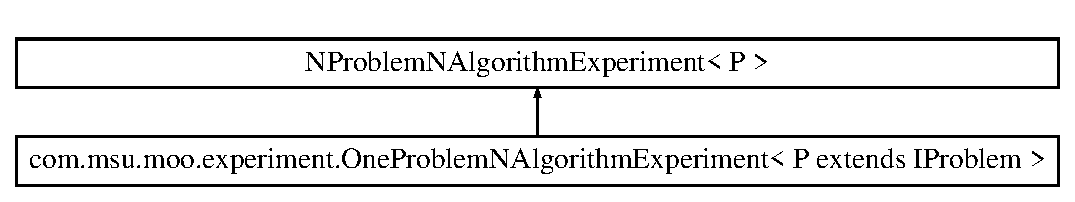
\includegraphics[height=2.000000cm]{classcom_1_1msu_1_1moo_1_1experiment_1_1OneProblemNAlgorithmExperiment_3_01P_01extends_01IProblem_01_4}
\end{center}
\end{figure}
\subsection*{Public Member Functions}
\begin{DoxyCompactItemize}
\item 
\hypertarget{classcom_1_1msu_1_1moo_1_1experiment_1_1OneProblemNAlgorithmExperiment_3_01P_01extends_01IProblem_01_4_ab0cb3c2001b86806de15944bdc796b48}{void {\bfseries report} ()}\label{classcom_1_1msu_1_1moo_1_1experiment_1_1OneProblemNAlgorithmExperiment_3_01P_01extends_01IProblem_01_4_ab0cb3c2001b86806de15944bdc796b48}

\end{DoxyCompactItemize}
\subsection*{Protected Member Functions}
\begin{DoxyCompactItemize}
\item 
\hypertarget{classcom_1_1msu_1_1moo_1_1experiment_1_1OneProblemNAlgorithmExperiment_3_01P_01extends_01IProblem_01_4_a44ade28cf960ba97dc5000335a284030}{abstract P {\bfseries get\-Problem} ()}\label{classcom_1_1msu_1_1moo_1_1experiment_1_1OneProblemNAlgorithmExperiment_3_01P_01extends_01IProblem_01_4_a44ade28cf960ba97dc5000335a284030}

\item 
\hypertarget{classcom_1_1msu_1_1moo_1_1experiment_1_1OneProblemNAlgorithmExperiment_3_01P_01extends_01IProblem_01_4_a34821a479b9f95094c10be7340b81614}{abstract \hyperlink{classcom_1_1msu_1_1moo_1_1model_1_1solution_1_1NonDominatedSolutionSet}{Non\-Dominated\-Solution\-Set} {\bfseries get\-True\-Front} ()}\label{classcom_1_1msu_1_1moo_1_1experiment_1_1OneProblemNAlgorithmExperiment_3_01P_01extends_01IProblem_01_4_a34821a479b9f95094c10be7340b81614}

\item 
\hypertarget{classcom_1_1msu_1_1moo_1_1experiment_1_1OneProblemNAlgorithmExperiment_3_01P_01extends_01IProblem_01_4_af101c14d9277ae9d947e612456fee50f}{Map$<$ P, \hyperlink{classcom_1_1msu_1_1moo_1_1model_1_1solution_1_1NonDominatedSolutionSet}{Non\-Dominated\-Solution\-Set} $>$ {\bfseries get\-Problems} ()}\label{classcom_1_1msu_1_1moo_1_1experiment_1_1OneProblemNAlgorithmExperiment_3_01P_01extends_01IProblem_01_4_af101c14d9277ae9d947e612456fee50f}

\end{DoxyCompactItemize}
\subsection*{Protected Attributes}
\begin{DoxyCompactItemize}
\item 
\hypertarget{classcom_1_1msu_1_1moo_1_1experiment_1_1OneProblemNAlgorithmExperiment_3_01P_01extends_01IProblem_01_4_aff43f342cc08af54e689b38093c8fac6}{P {\bfseries problem} = null}\label{classcom_1_1msu_1_1moo_1_1experiment_1_1OneProblemNAlgorithmExperiment_3_01P_01extends_01IProblem_01_4_aff43f342cc08af54e689b38093c8fac6}

\item 
\hypertarget{classcom_1_1msu_1_1moo_1_1experiment_1_1OneProblemNAlgorithmExperiment_3_01P_01extends_01IProblem_01_4_ae833679eb8a1a9a848d3fc1fa9eb72bf}{\hyperlink{classcom_1_1msu_1_1moo_1_1model_1_1solution_1_1NonDominatedSolutionSet}{Non\-Dominated\-Solution\-Set} {\bfseries true\-Front} = null}\label{classcom_1_1msu_1_1moo_1_1experiment_1_1OneProblemNAlgorithmExperiment_3_01P_01extends_01IProblem_01_4_ae833679eb8a1a9a848d3fc1fa9eb72bf}

\end{DoxyCompactItemize}


The documentation for this class was generated from the following file\-:\begin{DoxyCompactItemize}
\item 
src/main/java/com/msu/moo/experiment/One\-Problem\-N\-Algorithm\-Experiment.\-java\end{DoxyCompactItemize}

\hypertarget{classcom_1_1msu_1_1moo_1_1experiment_1_1OneProblemOneAlgorithmExperiment_3_01P_01extends_01IProblem_01_4}{\section{com.\-msu.\-moo.\-experiment.\-One\-Problem\-One\-Algorithm\-Experiment$<$ P extends I\-Problem $>$ Class Reference}
\label{classcom_1_1msu_1_1moo_1_1experiment_1_1OneProblemOneAlgorithmExperiment_3_01P_01extends_01IProblem_01_4}\index{com.\-msu.\-moo.\-experiment.\-One\-Problem\-One\-Algorithm\-Experiment$<$ P extends I\-Problem $>$@{com.\-msu.\-moo.\-experiment.\-One\-Problem\-One\-Algorithm\-Experiment$<$ P extends I\-Problem $>$}}
}
Inheritance diagram for com.\-msu.\-moo.\-experiment.\-One\-Problem\-One\-Algorithm\-Experiment$<$ P extends I\-Problem $>$\-:\begin{figure}[H]
\begin{center}
\leavevmode
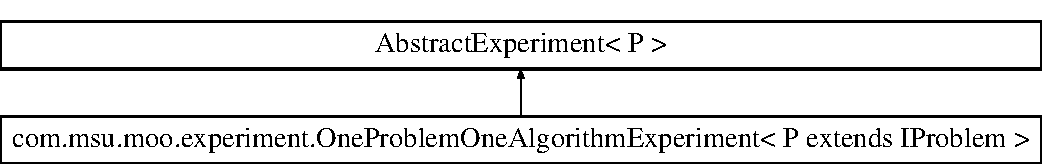
\includegraphics[height=2.000000cm]{classcom_1_1msu_1_1moo_1_1experiment_1_1OneProblemOneAlgorithmExperiment_3_01P_01extends_01IProblem_01_4}
\end{center}
\end{figure}
\subsection*{Public Member Functions}
\begin{DoxyCompactItemize}
\item 
\hypertarget{classcom_1_1msu_1_1moo_1_1experiment_1_1OneProblemOneAlgorithmExperiment_3_01P_01extends_01IProblem_01_4_a27714412a54115a1383557a614a87e8b}{void {\bfseries report} ()}\label{classcom_1_1msu_1_1moo_1_1experiment_1_1OneProblemOneAlgorithmExperiment_3_01P_01extends_01IProblem_01_4_a27714412a54115a1383557a614a87e8b}

\end{DoxyCompactItemize}
\subsection*{Protected Member Functions}
\begin{DoxyCompactItemize}
\item 
\hypertarget{classcom_1_1msu_1_1moo_1_1experiment_1_1OneProblemOneAlgorithmExperiment_3_01P_01extends_01IProblem_01_4_a4be8c0082941b96173984f1be64fdf60}{abstract I\-Algorithm$<$ P $>$ {\bfseries get\-Algorithm} ()}\label{classcom_1_1msu_1_1moo_1_1experiment_1_1OneProblemOneAlgorithmExperiment_3_01P_01extends_01IProblem_01_4_a4be8c0082941b96173984f1be64fdf60}

\item 
\hypertarget{classcom_1_1msu_1_1moo_1_1experiment_1_1OneProblemOneAlgorithmExperiment_3_01P_01extends_01IProblem_01_4_a66a9bca3285414a092d799b81e409e87}{abstract P {\bfseries get\-Problem} ()}\label{classcom_1_1msu_1_1moo_1_1experiment_1_1OneProblemOneAlgorithmExperiment_3_01P_01extends_01IProblem_01_4_a66a9bca3285414a092d799b81e409e87}

\item 
\hypertarget{classcom_1_1msu_1_1moo_1_1experiment_1_1OneProblemOneAlgorithmExperiment_3_01P_01extends_01IProblem_01_4_a51d161f8f6e72e32376879a0e478628c}{abstract \hyperlink{classcom_1_1msu_1_1moo_1_1model_1_1solution_1_1NonDominatedSolutionSet}{Non\-Dominated\-Solution\-Set} {\bfseries get\-True\-Front} ()}\label{classcom_1_1msu_1_1moo_1_1experiment_1_1OneProblemOneAlgorithmExperiment_3_01P_01extends_01IProblem_01_4_a51d161f8f6e72e32376879a0e478628c}

\item 
\hypertarget{classcom_1_1msu_1_1moo_1_1experiment_1_1OneProblemOneAlgorithmExperiment_3_01P_01extends_01IProblem_01_4_a31e2e2ddf1b0481a0d1bdb7b7e7f0153}{List$<$ I\-Algorithm$<$ P $>$ $>$ {\bfseries get\-Algorithms} ()}\label{classcom_1_1msu_1_1moo_1_1experiment_1_1OneProblemOneAlgorithmExperiment_3_01P_01extends_01IProblem_01_4_a31e2e2ddf1b0481a0d1bdb7b7e7f0153}

\item 
\hypertarget{classcom_1_1msu_1_1moo_1_1experiment_1_1OneProblemOneAlgorithmExperiment_3_01P_01extends_01IProblem_01_4_a56f5957cee781bc3ac517ae595d62a5a}{Map$<$ P, \hyperlink{classcom_1_1msu_1_1moo_1_1model_1_1solution_1_1NonDominatedSolutionSet}{Non\-Dominated\-Solution\-Set} $>$ {\bfseries get\-Problems} ()}\label{classcom_1_1msu_1_1moo_1_1experiment_1_1OneProblemOneAlgorithmExperiment_3_01P_01extends_01IProblem_01_4_a56f5957cee781bc3ac517ae595d62a5a}

\end{DoxyCompactItemize}
\subsection*{Protected Attributes}
\begin{DoxyCompactItemize}
\item 
\hypertarget{classcom_1_1msu_1_1moo_1_1experiment_1_1OneProblemOneAlgorithmExperiment_3_01P_01extends_01IProblem_01_4_a5e7eb55ed2fbd594059caa0cfc2286b1}{P {\bfseries problem} = null}\label{classcom_1_1msu_1_1moo_1_1experiment_1_1OneProblemOneAlgorithmExperiment_3_01P_01extends_01IProblem_01_4_a5e7eb55ed2fbd594059caa0cfc2286b1}

\item 
\hypertarget{classcom_1_1msu_1_1moo_1_1experiment_1_1OneProblemOneAlgorithmExperiment_3_01P_01extends_01IProblem_01_4_aa6923a1cfc9aa1d0de6c6b6e5e5de402}{\hyperlink{classcom_1_1msu_1_1moo_1_1model_1_1solution_1_1NonDominatedSolutionSet}{Non\-Dominated\-Solution\-Set} {\bfseries true\-Front} = null}\label{classcom_1_1msu_1_1moo_1_1experiment_1_1OneProblemOneAlgorithmExperiment_3_01P_01extends_01IProblem_01_4_aa6923a1cfc9aa1d0de6c6b6e5e5de402}

\item 
\hypertarget{classcom_1_1msu_1_1moo_1_1experiment_1_1OneProblemOneAlgorithmExperiment_3_01P_01extends_01IProblem_01_4_abab19d6f1451cb1eafd18460293c5d56}{I\-Algorithm$<$ P $>$ {\bfseries algorithm} = null}\label{classcom_1_1msu_1_1moo_1_1experiment_1_1OneProblemOneAlgorithmExperiment_3_01P_01extends_01IProblem_01_4_abab19d6f1451cb1eafd18460293c5d56}

\end{DoxyCompactItemize}


\subsection{Detailed Description}
This experiment is for plotting the resulting pareto fronts of one algorithm to have a look at different shapes or specific results.


\begin{DoxyParams}{Parameters}
{\em $<$\-P$>$} & Defines the kind of problem which should be part of this experiment \\
\hline
\end{DoxyParams}


The documentation for this class was generated from the following file\-:\begin{DoxyCompactItemize}
\item 
src/main/java/com/msu/moo/experiment/One\-Problem\-One\-Algorithm\-Experiment.\-java\end{DoxyCompactItemize}

\hypertarget{classcom_1_1msu_1_1moo_1_1operators_1_1crossover_1_1permutation_1_1OrderedCrossover_3_01T_01_4}{\section{com.\-msu.\-moo.\-operators.\-crossover.\-permutation.\-Ordered\-Crossover$<$ T $>$ Class Reference}
\label{classcom_1_1msu_1_1moo_1_1operators_1_1crossover_1_1permutation_1_1OrderedCrossover_3_01T_01_4}\index{com.\-msu.\-moo.\-operators.\-crossover.\-permutation.\-Ordered\-Crossover$<$ T $>$@{com.\-msu.\-moo.\-operators.\-crossover.\-permutation.\-Ordered\-Crossover$<$ T $>$}}
}
Inheritance diagram for com.\-msu.\-moo.\-operators.\-crossover.\-permutation.\-Ordered\-Crossover$<$ T $>$\-:\begin{figure}[H]
\begin{center}
\leavevmode
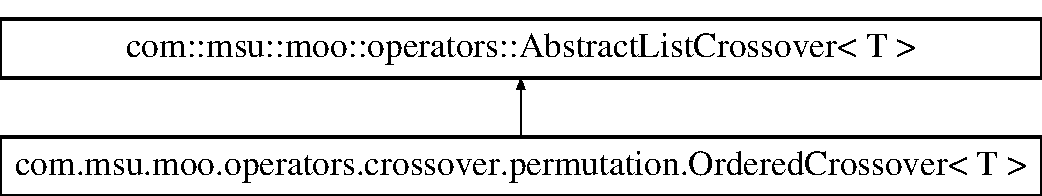
\includegraphics[height=2.000000cm]{classcom_1_1msu_1_1moo_1_1operators_1_1crossover_1_1permutation_1_1OrderedCrossover_3_01T_01_4}
\end{center}
\end{figure}
\subsection*{Protected Member Functions}
\begin{DoxyCompactItemize}
\item 
\hypertarget{classcom_1_1msu_1_1moo_1_1operators_1_1crossover_1_1permutation_1_1OrderedCrossover_3_01T_01_4_a1969cf216880631b581718a1c622f165}{List$<$ T $>$ {\bfseries crossover\-\_\-} (List$<$ T $>$ a, List$<$ T $>$ b, int lb, int ub)}\label{classcom_1_1msu_1_1moo_1_1operators_1_1crossover_1_1permutation_1_1OrderedCrossover_3_01T_01_4_a1969cf216880631b581718a1c622f165}

\item 
\hypertarget{classcom_1_1msu_1_1moo_1_1operators_1_1crossover_1_1permutation_1_1OrderedCrossover_3_01T_01_4_a2d2aa71c9ad0f559409a2fca60ded0b6}{List$<$ List$<$ T $>$ $>$ {\bfseries crossover\-Lists} (List$<$ T $>$ a, List$<$ T $>$ b)}\label{classcom_1_1msu_1_1moo_1_1operators_1_1crossover_1_1permutation_1_1OrderedCrossover_3_01T_01_4_a2d2aa71c9ad0f559409a2fca60ded0b6}

\end{DoxyCompactItemize}


The documentation for this class was generated from the following file\-:\begin{DoxyCompactItemize}
\item 
src/main/java/com/msu/moo/operators/crossover/permutation/Ordered\-Crossover.\-java\end{DoxyCompactItemize}

\hypertarget{classcom_1_1msu_1_1moo_1_1util_1_1Pair_3_01F_00_01S_01_4}{\section{com.\-msu.\-moo.\-util.\-Pair$<$ F, S $>$ Class Reference}
\label{classcom_1_1msu_1_1moo_1_1util_1_1Pair_3_01F_00_01S_01_4}\index{com.\-msu.\-moo.\-util.\-Pair$<$ F, S $>$@{com.\-msu.\-moo.\-util.\-Pair$<$ F, S $>$}}
}
\subsection*{Public Member Functions}
\begin{DoxyCompactItemize}
\item 
\hyperlink{classcom_1_1msu_1_1moo_1_1util_1_1Pair_3_01F_00_01S_01_4_a397b4d82aaefe176d1fb7f11d4f90f36}{Pair} (F first, S second)
\item 
boolean \hyperlink{classcom_1_1msu_1_1moo_1_1util_1_1Pair_3_01F_00_01S_01_4_afc75acfd72556f99a2bb8a95db6730cc}{equals} (Object o)
\item 
int \hyperlink{classcom_1_1msu_1_1moo_1_1util_1_1Pair_3_01F_00_01S_01_4_a8357b8dd6a4dea9b9d9fe3458e202bda}{hash\-Code} ()
\item 
\hypertarget{classcom_1_1msu_1_1moo_1_1util_1_1Pair_3_01F_00_01S_01_4_a588ae39cea02c367f99b619f8300ad4d}{String {\bfseries to\-String} ()}\label{classcom_1_1msu_1_1moo_1_1util_1_1Pair_3_01F_00_01S_01_4_a588ae39cea02c367f99b619f8300ad4d}

\end{DoxyCompactItemize}
\subsection*{Static Public Member Functions}
\begin{DoxyCompactItemize}
\item 
static$<$ A, B $>$ \hyperlink{classcom_1_1msu_1_1moo_1_1util_1_1Pair_3_01F_00_01S_01_4_a397b4d82aaefe176d1fb7f11d4f90f36}{Pair}$<$ A, B $>$ \hyperlink{classcom_1_1msu_1_1moo_1_1util_1_1Pair_3_01F_00_01S_01_4_a2c56a6a21d8d6a667415fc484548fc49}{create} (A a, B b)
\end{DoxyCompactItemize}
\subsection*{Public Attributes}
\begin{DoxyCompactItemize}
\item 
\hypertarget{classcom_1_1msu_1_1moo_1_1util_1_1Pair_3_01F_00_01S_01_4_a2a0d6a70275719bb02c5d5b2bcc3b270}{F {\bfseries first}}\label{classcom_1_1msu_1_1moo_1_1util_1_1Pair_3_01F_00_01S_01_4_a2a0d6a70275719bb02c5d5b2bcc3b270}

\item 
\hypertarget{classcom_1_1msu_1_1moo_1_1util_1_1Pair_3_01F_00_01S_01_4_aadab39e9459347f317aac90e13fda1e0}{S {\bfseries second}}\label{classcom_1_1msu_1_1moo_1_1util_1_1Pair_3_01F_00_01S_01_4_aadab39e9459347f317aac90e13fda1e0}

\end{DoxyCompactItemize}


\subsection{Detailed Description}
Container to ease passing around a tuple of two objects. This object provides a sensible implementation of \hyperlink{classcom_1_1msu_1_1moo_1_1util_1_1Pair_3_01F_00_01S_01_4_afc75acfd72556f99a2bb8a95db6730cc}{equals()}, returning true if \hyperlink{classcom_1_1msu_1_1moo_1_1util_1_1Pair_3_01F_00_01S_01_4_afc75acfd72556f99a2bb8a95db6730cc}{equals()} is true on each of the contained objects. 

\subsection{Constructor \& Destructor Documentation}
\hypertarget{classcom_1_1msu_1_1moo_1_1util_1_1Pair_3_01F_00_01S_01_4_a397b4d82aaefe176d1fb7f11d4f90f36}{\index{com\-::msu\-::moo\-::util\-::\-Pair$<$ F, S $>$@{com\-::msu\-::moo\-::util\-::\-Pair$<$ F, S $>$}!Pair@{Pair}}
\index{Pair@{Pair}!com::msu::moo::util::Pair< F, S >@{com\-::msu\-::moo\-::util\-::\-Pair$<$ F, S $>$}}
\subsubsection[{Pair}]{\setlength{\rightskip}{0pt plus 5cm}com.\-msu.\-moo.\-util.\-Pair$<$ F, S $>$.Pair (
\begin{DoxyParamCaption}
\item[{F}]{first, }
\item[{S}]{second}
\end{DoxyParamCaption}
)\hspace{0.3cm}{\ttfamily [inline]}}}\label{classcom_1_1msu_1_1moo_1_1util_1_1Pair_3_01F_00_01S_01_4_a397b4d82aaefe176d1fb7f11d4f90f36}
Constructor for a Pair. If either are null then \hyperlink{classcom_1_1msu_1_1moo_1_1util_1_1Pair_3_01F_00_01S_01_4_afc75acfd72556f99a2bb8a95db6730cc}{equals()} and \hyperlink{classcom_1_1msu_1_1moo_1_1util_1_1Pair_3_01F_00_01S_01_4_a8357b8dd6a4dea9b9d9fe3458e202bda}{hash\-Code()} will throw a Null\-Pointer\-Exception. 
\begin{DoxyParams}{Parameters}
{\em first} & the first object in the Pair \\
\hline
{\em second} & the second object in the pair \\
\hline
\end{DoxyParams}


\subsection{Member Function Documentation}
\hypertarget{classcom_1_1msu_1_1moo_1_1util_1_1Pair_3_01F_00_01S_01_4_a2c56a6a21d8d6a667415fc484548fc49}{\index{com\-::msu\-::moo\-::util\-::\-Pair$<$ F, S $>$@{com\-::msu\-::moo\-::util\-::\-Pair$<$ F, S $>$}!create@{create}}
\index{create@{create}!com::msu::moo::util::Pair< F, S >@{com\-::msu\-::moo\-::util\-::\-Pair$<$ F, S $>$}}
\subsubsection[{create}]{\setlength{\rightskip}{0pt plus 5cm}static $<$A,B$>$ {\bf Pair}$<$A, B$>$ com.\-msu.\-moo.\-util.\-Pair$<$ F, S $>$.create (
\begin{DoxyParamCaption}
\item[{A}]{a, }
\item[{B}]{b}
\end{DoxyParamCaption}
)\hspace{0.3cm}{\ttfamily [inline]}, {\ttfamily [static]}}}\label{classcom_1_1msu_1_1moo_1_1util_1_1Pair_3_01F_00_01S_01_4_a2c56a6a21d8d6a667415fc484548fc49}
Convenience method for creating an appropriately typed pair. 
\begin{DoxyParams}{Parameters}
{\em a} & the first object in the Pair \\
\hline
{\em b} & the second object in the pair \\
\hline
\end{DoxyParams}
\begin{DoxyReturn}{Returns}
a Pair that is templatized with the types of a and b 
\end{DoxyReturn}
\hypertarget{classcom_1_1msu_1_1moo_1_1util_1_1Pair_3_01F_00_01S_01_4_afc75acfd72556f99a2bb8a95db6730cc}{\index{com\-::msu\-::moo\-::util\-::\-Pair$<$ F, S $>$@{com\-::msu\-::moo\-::util\-::\-Pair$<$ F, S $>$}!equals@{equals}}
\index{equals@{equals}!com::msu::moo::util::Pair< F, S >@{com\-::msu\-::moo\-::util\-::\-Pair$<$ F, S $>$}}
\subsubsection[{equals}]{\setlength{\rightskip}{0pt plus 5cm}boolean com.\-msu.\-moo.\-util.\-Pair$<$ F, S $>$.equals (
\begin{DoxyParamCaption}
\item[{Object}]{o}
\end{DoxyParamCaption}
)\hspace{0.3cm}{\ttfamily [inline]}}}\label{classcom_1_1msu_1_1moo_1_1util_1_1Pair_3_01F_00_01S_01_4_afc75acfd72556f99a2bb8a95db6730cc}
Checks the two objects for equality by delegating to their respective \hyperlink{classcom_1_1msu_1_1moo_1_1util_1_1Pair_3_01F_00_01S_01_4_afc75acfd72556f99a2bb8a95db6730cc}{equals()} methods. 
\begin{DoxyParams}{Parameters}
{\em o} & the Pair to which this one is to be checked for equality \\
\hline
\end{DoxyParams}
\begin{DoxyReturn}{Returns}
true if the underlying objects of the Pair are both considered \hyperlink{classcom_1_1msu_1_1moo_1_1util_1_1Pair_3_01F_00_01S_01_4_afc75acfd72556f99a2bb8a95db6730cc}{equals()} 
\end{DoxyReturn}
\hypertarget{classcom_1_1msu_1_1moo_1_1util_1_1Pair_3_01F_00_01S_01_4_a8357b8dd6a4dea9b9d9fe3458e202bda}{\index{com\-::msu\-::moo\-::util\-::\-Pair$<$ F, S $>$@{com\-::msu\-::moo\-::util\-::\-Pair$<$ F, S $>$}!hash\-Code@{hash\-Code}}
\index{hash\-Code@{hash\-Code}!com::msu::moo::util::Pair< F, S >@{com\-::msu\-::moo\-::util\-::\-Pair$<$ F, S $>$}}
\subsubsection[{hash\-Code}]{\setlength{\rightskip}{0pt plus 5cm}int com.\-msu.\-moo.\-util.\-Pair$<$ F, S $>$.hash\-Code (
\begin{DoxyParamCaption}
{}
\end{DoxyParamCaption}
)\hspace{0.3cm}{\ttfamily [inline]}}}\label{classcom_1_1msu_1_1moo_1_1util_1_1Pair_3_01F_00_01S_01_4_a8357b8dd6a4dea9b9d9fe3458e202bda}
Compute a hash code using the hash codes of the underlying objects \begin{DoxyReturn}{Returns}
a hashcode of the Pair 
\end{DoxyReturn}


The documentation for this class was generated from the following file\-:\begin{DoxyCompactItemize}
\item 
src/main/java/com/msu/moo/util/Pair.\-java\end{DoxyCompactItemize}

\hypertarget{classcom_1_1msu_1_1moo_1_1operators_1_1crossover_1_1permutation_1_1PMXCrossover_3_01T_01_4}{\section{com.\-msu.\-moo.\-operators.\-crossover.\-permutation.\-P\-M\-X\-Crossover$<$ T $>$ Class Reference}
\label{classcom_1_1msu_1_1moo_1_1operators_1_1crossover_1_1permutation_1_1PMXCrossover_3_01T_01_4}\index{com.\-msu.\-moo.\-operators.\-crossover.\-permutation.\-P\-M\-X\-Crossover$<$ T $>$@{com.\-msu.\-moo.\-operators.\-crossover.\-permutation.\-P\-M\-X\-Crossover$<$ T $>$}}
}
Inheritance diagram for com.\-msu.\-moo.\-operators.\-crossover.\-permutation.\-P\-M\-X\-Crossover$<$ T $>$\-:\begin{figure}[H]
\begin{center}
\leavevmode
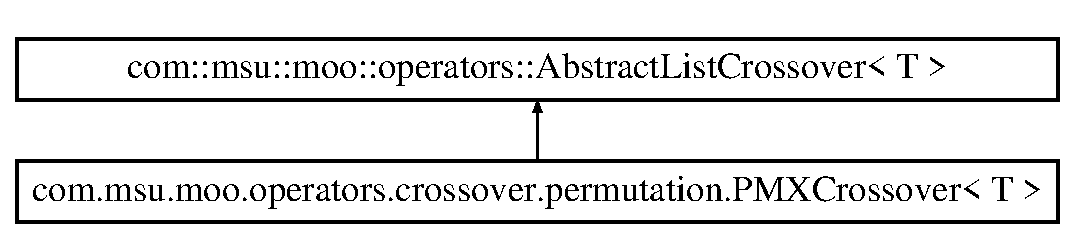
\includegraphics[height=2.000000cm]{classcom_1_1msu_1_1moo_1_1operators_1_1crossover_1_1permutation_1_1PMXCrossover_3_01T_01_4}
\end{center}
\end{figure}
\subsection*{Protected Member Functions}
\begin{DoxyCompactItemize}
\item 
\hypertarget{classcom_1_1msu_1_1moo_1_1operators_1_1crossover_1_1permutation_1_1PMXCrossover_3_01T_01_4_a10e8e4b1363f0ce2921ad38b88f81bbe}{List$<$ T $>$ {\bfseries crossover\-\_\-} (List$<$ T $>$ a, List$<$ T $>$ b, int lb, int ub)}\label{classcom_1_1msu_1_1moo_1_1operators_1_1crossover_1_1permutation_1_1PMXCrossover_3_01T_01_4_a10e8e4b1363f0ce2921ad38b88f81bbe}

\item 
\hypertarget{classcom_1_1msu_1_1moo_1_1operators_1_1crossover_1_1permutation_1_1PMXCrossover_3_01T_01_4_a099893f6f25f515ea94e9042ca87f515}{List$<$ List$<$ T $>$ $>$ {\bfseries crossover\-Lists} (List$<$ T $>$ a, List$<$ T $>$ b)}\label{classcom_1_1msu_1_1moo_1_1operators_1_1crossover_1_1permutation_1_1PMXCrossover_3_01T_01_4_a099893f6f25f515ea94e9042ca87f515}

\end{DoxyCompactItemize}


The documentation for this class was generated from the following file\-:\begin{DoxyCompactItemize}
\item 
src/main/java/com/msu/moo/operators/crossover/permutation/P\-M\-X\-Crossover.\-java\end{DoxyCompactItemize}

\hypertarget{classcom_1_1msu_1_1moo_1_1operators_1_1mutation_1_1PolynomialMutation}{\section{com.\-msu.\-moo.\-operators.\-mutation.\-Polynomial\-Mutation Class Reference}
\label{classcom_1_1msu_1_1moo_1_1operators_1_1mutation_1_1PolynomialMutation}\index{com.\-msu.\-moo.\-operators.\-mutation.\-Polynomial\-Mutation@{com.\-msu.\-moo.\-operators.\-mutation.\-Polynomial\-Mutation}}
}
Inheritance diagram for com.\-msu.\-moo.\-operators.\-mutation.\-Polynomial\-Mutation\-:\begin{figure}[H]
\begin{center}
\leavevmode
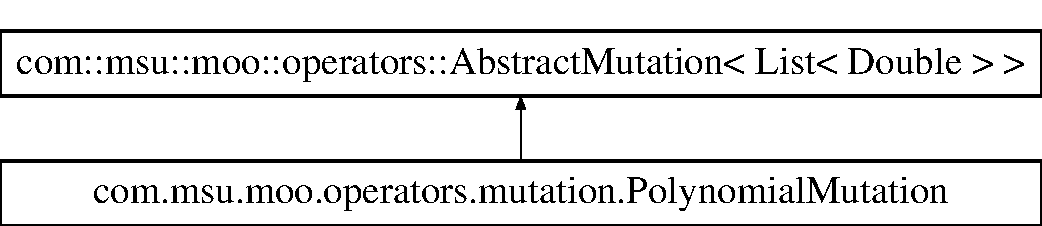
\includegraphics[height=2.000000cm]{classcom_1_1msu_1_1moo_1_1operators_1_1mutation_1_1PolynomialMutation}
\end{center}
\end{figure}
\subsection*{Public Member Functions}
\begin{DoxyCompactItemize}
\item 
\hyperlink{classcom_1_1msu_1_1moo_1_1operators_1_1mutation_1_1PolynomialMutation_ae8ba9e14d445f820b53b04e4b1e644fc}{Polynomial\-Mutation} ()
\item 
\hyperlink{classcom_1_1msu_1_1moo_1_1operators_1_1mutation_1_1PolynomialMutation_a265b9ed40d686047a56521bbed462c96}{Polynomial\-Mutation} (Double \hyperlink{classcom_1_1msu_1_1moo_1_1operators_1_1mutation_1_1PolynomialMutation_ac70d8ffc1d71d3d3c28554eecebf69db}{probability})
\item 
\hypertarget{classcom_1_1msu_1_1moo_1_1operators_1_1mutation_1_1PolynomialMutation_a8432510b01750db3c0b412f38ce984dd}{{\bfseries Polynomial\-Mutation} (Double\mbox{[}$\,$\mbox{]} \hyperlink{classcom_1_1msu_1_1moo_1_1operators_1_1mutation_1_1PolynomialMutation_ab96c1108fc7a705fa962bdc611fcf152}{range})}\label{classcom_1_1msu_1_1moo_1_1operators_1_1mutation_1_1PolynomialMutation_a8432510b01750db3c0b412f38ce984dd}

\item 
\hypertarget{classcom_1_1msu_1_1moo_1_1operators_1_1mutation_1_1PolynomialMutation_aef773cf9e54603246e065c4fd4931633}{void {\bfseries set\-Range} (Double\mbox{[}$\,$\mbox{]} \hyperlink{classcom_1_1msu_1_1moo_1_1operators_1_1mutation_1_1PolynomialMutation_ab96c1108fc7a705fa962bdc611fcf152}{range})}\label{classcom_1_1msu_1_1moo_1_1operators_1_1mutation_1_1PolynomialMutation_aef773cf9e54603246e065c4fd4931633}

\end{DoxyCompactItemize}
\subsection*{Protected Member Functions}
\begin{DoxyCompactItemize}
\item 
\hypertarget{classcom_1_1msu_1_1moo_1_1operators_1_1mutation_1_1PolynomialMutation_acd61972e04896b67faa1feba0f1454c5}{void {\bfseries mutate\-\_\-} (List$<$ Double $>$ b)}\label{classcom_1_1msu_1_1moo_1_1operators_1_1mutation_1_1PolynomialMutation_acd61972e04896b67faa1feba0f1454c5}

\end{DoxyCompactItemize}
\subsection*{Protected Attributes}
\begin{DoxyCompactItemize}
\item 
\hypertarget{classcom_1_1msu_1_1moo_1_1operators_1_1mutation_1_1PolynomialMutation_ac70d8ffc1d71d3d3c28554eecebf69db}{Double \hyperlink{classcom_1_1msu_1_1moo_1_1operators_1_1mutation_1_1PolynomialMutation_ac70d8ffc1d71d3d3c28554eecebf69db}{probability} = null}\label{classcom_1_1msu_1_1moo_1_1operators_1_1mutation_1_1PolynomialMutation_ac70d8ffc1d71d3d3c28554eecebf69db}

\begin{DoxyCompactList}\small\item\em the probability that a bit is changed \end{DoxyCompactList}\item 
\hypertarget{classcom_1_1msu_1_1moo_1_1operators_1_1mutation_1_1PolynomialMutation_ab96c1108fc7a705fa962bdc611fcf152}{Double\mbox{[}$\,$\mbox{]} \hyperlink{classcom_1_1msu_1_1moo_1_1operators_1_1mutation_1_1PolynomialMutation_ab96c1108fc7a705fa962bdc611fcf152}{range} = new Double\mbox{[}$\,$\mbox{]} \{Double.\-M\-I\-N\-\_\-\-V\-A\-L\-U\-E, Double.\-M\-A\-X\-\_\-\-V\-A\-L\-U\-E\}}\label{classcom_1_1msu_1_1moo_1_1operators_1_1mutation_1_1PolynomialMutation_ab96c1108fc7a705fa962bdc611fcf152}

\begin{DoxyCompactList}\small\item\em range of the results \end{DoxyCompactList}\end{DoxyCompactItemize}


\subsection{Constructor \& Destructor Documentation}
\hypertarget{classcom_1_1msu_1_1moo_1_1operators_1_1mutation_1_1PolynomialMutation_ae8ba9e14d445f820b53b04e4b1e644fc}{\index{com\-::msu\-::moo\-::operators\-::mutation\-::\-Polynomial\-Mutation@{com\-::msu\-::moo\-::operators\-::mutation\-::\-Polynomial\-Mutation}!Polynomial\-Mutation@{Polynomial\-Mutation}}
\index{Polynomial\-Mutation@{Polynomial\-Mutation}!com::msu::moo::operators::mutation::PolynomialMutation@{com\-::msu\-::moo\-::operators\-::mutation\-::\-Polynomial\-Mutation}}
\subsubsection[{Polynomial\-Mutation}]{\setlength{\rightskip}{0pt plus 5cm}com.\-msu.\-moo.\-operators.\-mutation.\-Polynomial\-Mutation.\-Polynomial\-Mutation (
\begin{DoxyParamCaption}
{}
\end{DoxyParamCaption}
)\hspace{0.3cm}{\ttfamily [inline]}}}\label{classcom_1_1msu_1_1moo_1_1operators_1_1mutation_1_1PolynomialMutation_ae8ba9e14d445f820b53b04e4b1e644fc}
Normal constructor with dynamic probability \hypertarget{classcom_1_1msu_1_1moo_1_1operators_1_1mutation_1_1PolynomialMutation_a265b9ed40d686047a56521bbed462c96}{\index{com\-::msu\-::moo\-::operators\-::mutation\-::\-Polynomial\-Mutation@{com\-::msu\-::moo\-::operators\-::mutation\-::\-Polynomial\-Mutation}!Polynomial\-Mutation@{Polynomial\-Mutation}}
\index{Polynomial\-Mutation@{Polynomial\-Mutation}!com::msu::moo::operators::mutation::PolynomialMutation@{com\-::msu\-::moo\-::operators\-::mutation\-::\-Polynomial\-Mutation}}
\subsubsection[{Polynomial\-Mutation}]{\setlength{\rightskip}{0pt plus 5cm}com.\-msu.\-moo.\-operators.\-mutation.\-Polynomial\-Mutation.\-Polynomial\-Mutation (
\begin{DoxyParamCaption}
\item[{Double}]{probability}
\end{DoxyParamCaption}
)\hspace{0.3cm}{\ttfamily [inline]}}}\label{classcom_1_1msu_1_1moo_1_1operators_1_1mutation_1_1PolynomialMutation_a265b9ed40d686047a56521bbed462c96}
Constructor which fixes the probability for all inputs. 
\begin{DoxyParams}{Parameters}
{\em probability} & that a bit is changed \\
\hline
\end{DoxyParams}


The documentation for this class was generated from the following file\-:\begin{DoxyCompactItemize}
\item 
src/main/java/com/msu/moo/operators/mutation/Polynomial\-Mutation.\-java\end{DoxyCompactItemize}

\hypertarget{classcom_1_1msu_1_1moo_1_1util_1_1Random}{\section{com.\-msu.\-moo.\-util.\-Random Class Reference}
\label{classcom_1_1msu_1_1moo_1_1util_1_1Random}\index{com.\-msu.\-moo.\-util.\-Random@{com.\-msu.\-moo.\-util.\-Random}}
}
\subsection*{Public Member Functions}
\begin{DoxyCompactItemize}
\item 
Integer \hyperlink{classcom_1_1msu_1_1moo_1_1util_1_1Random_af3b71ad155c4513eaaa8b1556767ff26}{next\-Int} (int max)
\item 
Integer \hyperlink{classcom_1_1msu_1_1moo_1_1util_1_1Random_ac9e121017e7630611ecfbc7e440cf7a9}{next\-Int} (int min, int max)
\item 
Double \hyperlink{classcom_1_1msu_1_1moo_1_1util_1_1Random_a32a22b76a2c1daad772e43957dd6dd7a}{next\-Double} ()
\item 
Double \hyperlink{classcom_1_1msu_1_1moo_1_1util_1_1Random_ab5d98f443d08e6809931e62a5fcf83ae}{next\-Double} (double min, double max)
\item 
void \hyperlink{classcom_1_1msu_1_1moo_1_1util_1_1Random_a73872b4d8d1973314c787070c813f33c}{set\-Seed} (long \hyperlink{classcom_1_1msu_1_1moo_1_1util_1_1Random_ae2ac6497beef04b12a28cb6e4706b57c}{seed})
\item 
long \hyperlink{classcom_1_1msu_1_1moo_1_1util_1_1Random_a632e2424c313b2c62019935834aa40e5}{get\-Seed} ()
\item 
\hypertarget{classcom_1_1msu_1_1moo_1_1util_1_1Random_a6ad21bc89260ca065844756e8af52904}{void {\bfseries shuffle} (List$<$?$>$ c)}\label{classcom_1_1msu_1_1moo_1_1util_1_1Random_a6ad21bc89260ca065844756e8af52904}

\end{DoxyCompactItemize}
\subsection*{Static Public Member Functions}
\begin{DoxyCompactItemize}
\item 
static \hyperlink{classcom_1_1msu_1_1moo_1_1util_1_1Random}{Random} \hyperlink{classcom_1_1msu_1_1moo_1_1util_1_1Random_aaa20005ec38b5944262c79c06d92ab62}{get\-Instance} ()
\end{DoxyCompactItemize}
\subsection*{Protected Attributes}
\begin{DoxyCompactItemize}
\item 
\hypertarget{classcom_1_1msu_1_1moo_1_1util_1_1Random_ae2ac6497beef04b12a28cb6e4706b57c}{long \hyperlink{classcom_1_1msu_1_1moo_1_1util_1_1Random_ae2ac6497beef04b12a28cb6e4706b57c}{seed}}\label{classcom_1_1msu_1_1moo_1_1util_1_1Random_ae2ac6497beef04b12a28cb6e4706b57c}

\begin{DoxyCompactList}\small\item\em current seed which is set to the random object \end{DoxyCompactList}\item 
\hypertarget{classcom_1_1msu_1_1moo_1_1util_1_1Random_ae1ad9be1fc9e28ccbcadfa8355fe082f}{java.\-util.\-Random \hyperlink{classcom_1_1msu_1_1moo_1_1util_1_1Random_ae1ad9be1fc9e28ccbcadfa8355fe082f}{r}}\label{classcom_1_1msu_1_1moo_1_1util_1_1Random_ae1ad9be1fc9e28ccbcadfa8355fe082f}

\begin{DoxyCompactList}\small\item\em the current random object \end{DoxyCompactList}\end{DoxyCompactItemize}
\subsection*{Static Protected Attributes}
\begin{DoxyCompactItemize}
\item 
\hypertarget{classcom_1_1msu_1_1moo_1_1util_1_1Random_a711b7af562b8f9f3d1e7ac04a5063aa0}{static \hyperlink{classcom_1_1msu_1_1moo_1_1util_1_1Random}{Random} \hyperlink{classcom_1_1msu_1_1moo_1_1util_1_1Random_a711b7af562b8f9f3d1e7ac04a5063aa0}{instance}}\label{classcom_1_1msu_1_1moo_1_1util_1_1Random_a711b7af562b8f9f3d1e7ac04a5063aa0}

\begin{DoxyCompactList}\small\item\em the current singleton instance \end{DoxyCompactList}\end{DoxyCompactItemize}


\subsection{Detailed Description}
This is a random generator which provides some advanced random methods and uses the Single\-Pattern to be created. 

\subsection{Member Function Documentation}
\hypertarget{classcom_1_1msu_1_1moo_1_1util_1_1Random_aaa20005ec38b5944262c79c06d92ab62}{\index{com\-::msu\-::moo\-::util\-::\-Random@{com\-::msu\-::moo\-::util\-::\-Random}!get\-Instance@{get\-Instance}}
\index{get\-Instance@{get\-Instance}!com::msu::moo::util::Random@{com\-::msu\-::moo\-::util\-::\-Random}}
\subsubsection[{get\-Instance}]{\setlength{\rightskip}{0pt plus 5cm}static {\bf Random} com.\-msu.\-moo.\-util.\-Random.\-get\-Instance (
\begin{DoxyParamCaption}
{}
\end{DoxyParamCaption}
)\hspace{0.3cm}{\ttfamily [inline]}, {\ttfamily [static]}}}\label{classcom_1_1msu_1_1moo_1_1util_1_1Random_aaa20005ec38b5944262c79c06d92ab62}
Method to create or return the singleton object. \begin{DoxyReturn}{Returns}

\end{DoxyReturn}
\hypertarget{classcom_1_1msu_1_1moo_1_1util_1_1Random_a632e2424c313b2c62019935834aa40e5}{\index{com\-::msu\-::moo\-::util\-::\-Random@{com\-::msu\-::moo\-::util\-::\-Random}!get\-Seed@{get\-Seed}}
\index{get\-Seed@{get\-Seed}!com::msu::moo::util::Random@{com\-::msu\-::moo\-::util\-::\-Random}}
\subsubsection[{get\-Seed}]{\setlength{\rightskip}{0pt plus 5cm}long com.\-msu.\-moo.\-util.\-Random.\-get\-Seed (
\begin{DoxyParamCaption}
{}
\end{DoxyParamCaption}
)\hspace{0.3cm}{\ttfamily [inline]}}}\label{classcom_1_1msu_1_1moo_1_1util_1_1Random_a632e2424c313b2c62019935834aa40e5}
Return the seed which was previously set \hypertarget{classcom_1_1msu_1_1moo_1_1util_1_1Random_a32a22b76a2c1daad772e43957dd6dd7a}{\index{com\-::msu\-::moo\-::util\-::\-Random@{com\-::msu\-::moo\-::util\-::\-Random}!next\-Double@{next\-Double}}
\index{next\-Double@{next\-Double}!com::msu::moo::util::Random@{com\-::msu\-::moo\-::util\-::\-Random}}
\subsubsection[{next\-Double}]{\setlength{\rightskip}{0pt plus 5cm}Double com.\-msu.\-moo.\-util.\-Random.\-next\-Double (
\begin{DoxyParamCaption}
{}
\end{DoxyParamCaption}
)\hspace{0.3cm}{\ttfamily [inline]}}}\label{classcom_1_1msu_1_1moo_1_1util_1_1Random_a32a22b76a2c1daad772e43957dd6dd7a}
Create a double value between 0 and 1. \hypertarget{classcom_1_1msu_1_1moo_1_1util_1_1Random_ab5d98f443d08e6809931e62a5fcf83ae}{\index{com\-::msu\-::moo\-::util\-::\-Random@{com\-::msu\-::moo\-::util\-::\-Random}!next\-Double@{next\-Double}}
\index{next\-Double@{next\-Double}!com::msu::moo::util::Random@{com\-::msu\-::moo\-::util\-::\-Random}}
\subsubsection[{next\-Double}]{\setlength{\rightskip}{0pt plus 5cm}Double com.\-msu.\-moo.\-util.\-Random.\-next\-Double (
\begin{DoxyParamCaption}
\item[{double}]{min, }
\item[{double}]{max}
\end{DoxyParamCaption}
)\hspace{0.3cm}{\ttfamily [inline]}}}\label{classcom_1_1msu_1_1moo_1_1util_1_1Random_ab5d98f443d08e6809931e62a5fcf83ae}
Create a double value in range \hypertarget{classcom_1_1msu_1_1moo_1_1util_1_1Random_af3b71ad155c4513eaaa8b1556767ff26}{\index{com\-::msu\-::moo\-::util\-::\-Random@{com\-::msu\-::moo\-::util\-::\-Random}!next\-Int@{next\-Int}}
\index{next\-Int@{next\-Int}!com::msu::moo::util::Random@{com\-::msu\-::moo\-::util\-::\-Random}}
\subsubsection[{next\-Int}]{\setlength{\rightskip}{0pt plus 5cm}Integer com.\-msu.\-moo.\-util.\-Random.\-next\-Int (
\begin{DoxyParamCaption}
\item[{int}]{max}
\end{DoxyParamCaption}
)\hspace{0.3cm}{\ttfamily [inline]}}}\label{classcom_1_1msu_1_1moo_1_1util_1_1Random_af3b71ad155c4513eaaa8b1556767ff26}
Create an Integer without range \hypertarget{classcom_1_1msu_1_1moo_1_1util_1_1Random_ac9e121017e7630611ecfbc7e440cf7a9}{\index{com\-::msu\-::moo\-::util\-::\-Random@{com\-::msu\-::moo\-::util\-::\-Random}!next\-Int@{next\-Int}}
\index{next\-Int@{next\-Int}!com::msu::moo::util::Random@{com\-::msu\-::moo\-::util\-::\-Random}}
\subsubsection[{next\-Int}]{\setlength{\rightskip}{0pt plus 5cm}Integer com.\-msu.\-moo.\-util.\-Random.\-next\-Int (
\begin{DoxyParamCaption}
\item[{int}]{min, }
\item[{int}]{max}
\end{DoxyParamCaption}
)\hspace{0.3cm}{\ttfamily [inline]}}}\label{classcom_1_1msu_1_1moo_1_1util_1_1Random_ac9e121017e7630611ecfbc7e440cf7a9}
Create an Integer in range \hypertarget{classcom_1_1msu_1_1moo_1_1util_1_1Random_a73872b4d8d1973314c787070c813f33c}{\index{com\-::msu\-::moo\-::util\-::\-Random@{com\-::msu\-::moo\-::util\-::\-Random}!set\-Seed@{set\-Seed}}
\index{set\-Seed@{set\-Seed}!com::msu::moo::util::Random@{com\-::msu\-::moo\-::util\-::\-Random}}
\subsubsection[{set\-Seed}]{\setlength{\rightskip}{0pt plus 5cm}void com.\-msu.\-moo.\-util.\-Random.\-set\-Seed (
\begin{DoxyParamCaption}
\item[{long}]{seed}
\end{DoxyParamCaption}
)\hspace{0.3cm}{\ttfamily [inline]}}}\label{classcom_1_1msu_1_1moo_1_1util_1_1Random_a73872b4d8d1973314c787070c813f33c}
Set the seed of the object 

The documentation for this class was generated from the following file\-:\begin{DoxyCompactItemize}
\item 
src/main/java/com/msu/moo/util/Random.\-java\end{DoxyCompactItemize}

\hypertarget{classcom_1_1msu_1_1moo_1_1algorithms_1_1RandomSearch_3_01V_01extends_01IVariable_00_01P_01extends_01IProblem_01_4}{\section{com.\-msu.\-moo.\-algorithms.\-Random\-Search$<$ V extends I\-Variable, P extends I\-Problem $>$ Class Reference}
\label{classcom_1_1msu_1_1moo_1_1algorithms_1_1RandomSearch_3_01V_01extends_01IVariable_00_01P_01extends_01IProblem_01_4}\index{com.\-msu.\-moo.\-algorithms.\-Random\-Search$<$ V extends I\-Variable, P extends I\-Problem $>$@{com.\-msu.\-moo.\-algorithms.\-Random\-Search$<$ V extends I\-Variable, P extends I\-Problem $>$}}
}
Inheritance diagram for com.\-msu.\-moo.\-algorithms.\-Random\-Search$<$ V extends I\-Variable, P extends I\-Problem $>$\-:\begin{figure}[H]
\begin{center}
\leavevmode
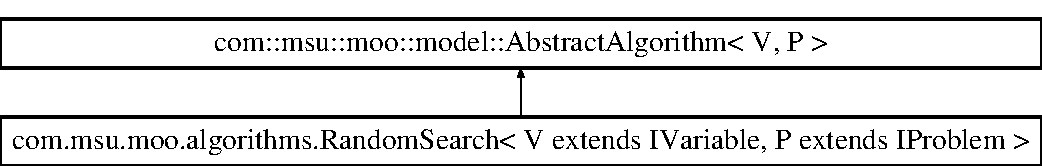
\includegraphics[height=2.000000cm]{classcom_1_1msu_1_1moo_1_1algorithms_1_1RandomSearch_3_01V_01extends_01IVariable_00_01P_01extends_01IProblem_01_4}
\end{center}
\end{figure}
\subsection*{Public Member Functions}
\begin{DoxyCompactItemize}
\item 
\hypertarget{classcom_1_1msu_1_1moo_1_1algorithms_1_1RandomSearch_3_01V_01extends_01IVariable_00_01P_01extends_01IProblem_01_4_a1b39ee9d053467c6a7c98a1f1e2b5fd6}{{\bfseries Random\-Search} (Variable\-Factory$<$ V, P $>$ factory)}\label{classcom_1_1msu_1_1moo_1_1algorithms_1_1RandomSearch_3_01V_01extends_01IVariable_00_01P_01extends_01IProblem_01_4_a1b39ee9d053467c6a7c98a1f1e2b5fd6}

\end{DoxyCompactItemize}
\subsection*{Protected Member Functions}
\begin{DoxyCompactItemize}
\item 
\hypertarget{classcom_1_1msu_1_1moo_1_1algorithms_1_1RandomSearch_3_01V_01extends_01IVariable_00_01P_01extends_01IProblem_01_4_a733715ef809343fd9a55bbeba9124c76}{void {\bfseries initialize} ()}\label{classcom_1_1msu_1_1moo_1_1algorithms_1_1RandomSearch_3_01V_01extends_01IVariable_00_01P_01extends_01IProblem_01_4_a733715ef809343fd9a55bbeba9124c76}

\item 
\hypertarget{classcom_1_1msu_1_1moo_1_1algorithms_1_1RandomSearch_3_01V_01extends_01IVariable_00_01P_01extends_01IProblem_01_4_abd3ce44b2b5cf65601d0291c2280005b}{void {\bfseries next} ()}\label{classcom_1_1msu_1_1moo_1_1algorithms_1_1RandomSearch_3_01V_01extends_01IVariable_00_01P_01extends_01IProblem_01_4_abd3ce44b2b5cf65601d0291c2280005b}

\item 
\hypertarget{classcom_1_1msu_1_1moo_1_1algorithms_1_1RandomSearch_3_01V_01extends_01IVariable_00_01P_01extends_01IProblem_01_4_ae9678352c27c53de569664879dde5353}{\hyperlink{classcom_1_1msu_1_1moo_1_1model_1_1solution_1_1NonDominatedSolutionSet}{Non\-Dominated\-Solution\-Set} {\bfseries get\-Result} ()}\label{classcom_1_1msu_1_1moo_1_1algorithms_1_1RandomSearch_3_01V_01extends_01IVariable_00_01P_01extends_01IProblem_01_4_ae9678352c27c53de569664879dde5353}

\end{DoxyCompactItemize}
\subsection*{Protected Attributes}
\begin{DoxyCompactItemize}
\item 
\hypertarget{classcom_1_1msu_1_1moo_1_1algorithms_1_1RandomSearch_3_01V_01extends_01IVariable_00_01P_01extends_01IProblem_01_4_adb6dda7177bfe4b7e8690d7fd15685d0}{\hyperlink{classcom_1_1msu_1_1moo_1_1model_1_1solution_1_1NonDominatedSolutionSet}{Non\-Dominated\-Solution\-Set} \hyperlink{classcom_1_1msu_1_1moo_1_1algorithms_1_1RandomSearch_3_01V_01extends_01IVariable_00_01P_01extends_01IProblem_01_4_adb6dda7177bfe4b7e8690d7fd15685d0}{set}}\label{classcom_1_1msu_1_1moo_1_1algorithms_1_1RandomSearch_3_01V_01extends_01IVariable_00_01P_01extends_01IProblem_01_4_adb6dda7177bfe4b7e8690d7fd15685d0}

\begin{DoxyCompactList}\small\item\em the final result set \end{DoxyCompactList}\item 
\hypertarget{classcom_1_1msu_1_1moo_1_1algorithms_1_1RandomSearch_3_01V_01extends_01IVariable_00_01P_01extends_01IProblem_01_4_a99e93b6813c3ed7f5c1efccd6b56da90}{int \hyperlink{classcom_1_1msu_1_1moo_1_1algorithms_1_1RandomSearch_3_01V_01extends_01IVariable_00_01P_01extends_01IProblem_01_4_a99e93b6813c3ed7f5c1efccd6b56da90}{evals\-Per\-Next} = 100}\label{classcom_1_1msu_1_1moo_1_1algorithms_1_1RandomSearch_3_01V_01extends_01IVariable_00_01P_01extends_01IProblem_01_4_a99e93b6813c3ed7f5c1efccd6b56da90}

\begin{DoxyCompactList}\small\item\em how many evaluations per next \end{DoxyCompactList}\end{DoxyCompactItemize}


The documentation for this class was generated from the following file\-:\begin{DoxyCompactItemize}
\item 
src/main/java/com/msu/moo/algorithms/Random\-Search.\-java\end{DoxyCompactItemize}

\hypertarget{classcom_1_1msu_1_1moo_1_1util_1_1Range_3_01T_01extends_01Comparable_3_01T_01_4_01_4}{\section{com.\-msu.\-moo.\-util.\-Range$<$ T extends Comparable$<$ T $>$ $>$ Class Reference}
\label{classcom_1_1msu_1_1moo_1_1util_1_1Range_3_01T_01extends_01Comparable_3_01T_01_4_01_4}\index{com.\-msu.\-moo.\-util.\-Range$<$ T extends Comparable$<$ T $>$ $>$@{com.\-msu.\-moo.\-util.\-Range$<$ T extends Comparable$<$ T $>$ $>$}}
}
\subsection*{Public Member Functions}
\begin{DoxyCompactItemize}
\item 
\hypertarget{classcom_1_1msu_1_1moo_1_1util_1_1Range_3_01T_01extends_01Comparable_3_01T_01_4_01_4_a34c556c5672d7b270a8fa0d33b61c97a}{void {\bfseries add} (List$<$ T $>$ l)}\label{classcom_1_1msu_1_1moo_1_1util_1_1Range_3_01T_01extends_01Comparable_3_01T_01_4_01_4_a34c556c5672d7b270a8fa0d33b61c97a}

\item 
\hypertarget{classcom_1_1msu_1_1moo_1_1util_1_1Range_3_01T_01extends_01Comparable_3_01T_01_4_01_4_a0dff5e8281b4940cdcb98803cd34906b}{List$<$ Pair$<$ T, T $>$ $>$ {\bfseries get} ()}\label{classcom_1_1msu_1_1moo_1_1util_1_1Range_3_01T_01extends_01Comparable_3_01T_01_4_01_4_a0dff5e8281b4940cdcb98803cd34906b}

\item 
\hypertarget{classcom_1_1msu_1_1moo_1_1util_1_1Range_3_01T_01extends_01Comparable_3_01T_01_4_01_4_a08c0a4badf7ee0296c2b73a8851af3d7}{T {\bfseries get\-Minimum} (int n)}\label{classcom_1_1msu_1_1moo_1_1util_1_1Range_3_01T_01extends_01Comparable_3_01T_01_4_01_4_a08c0a4badf7ee0296c2b73a8851af3d7}

\item 
\hypertarget{classcom_1_1msu_1_1moo_1_1util_1_1Range_3_01T_01extends_01Comparable_3_01T_01_4_01_4_ade94b2e3fe5ac0df02abd205bf23d90b}{T {\bfseries get\-Maximum} (int n)}\label{classcom_1_1msu_1_1moo_1_1util_1_1Range_3_01T_01extends_01Comparable_3_01T_01_4_01_4_ade94b2e3fe5ac0df02abd205bf23d90b}

\item 
\hypertarget{classcom_1_1msu_1_1moo_1_1util_1_1Range_3_01T_01extends_01Comparable_3_01T_01_4_01_4_ae8071b45d598a8802d7f40e72d376f8d}{int {\bfseries size} ()}\label{classcom_1_1msu_1_1moo_1_1util_1_1Range_3_01T_01extends_01Comparable_3_01T_01_4_01_4_ae8071b45d598a8802d7f40e72d376f8d}

\end{DoxyCompactItemize}
\subsection*{Protected Attributes}
\begin{DoxyCompactItemize}
\item 
\hypertarget{classcom_1_1msu_1_1moo_1_1util_1_1Range_3_01T_01extends_01Comparable_3_01T_01_4_01_4_a5ca963fc0452d874af5fcd4f4f9a14c9}{List$<$ Pair$<$ T, T $>$ $>$ {\bfseries ranges} = null}\label{classcom_1_1msu_1_1moo_1_1util_1_1Range_3_01T_01extends_01Comparable_3_01T_01_4_01_4_a5ca963fc0452d874af5fcd4f4f9a14c9}

\end{DoxyCompactItemize}


\subsection{Detailed Description}
This class allows to save always the range of a collection of points.


\begin{DoxyParams}{Parameters}
{\em $<$\-T$>$} & type of the points. \\
\hline
\end{DoxyParams}


The documentation for this class was generated from the following file\-:\begin{DoxyCompactItemize}
\item 
src/main/java/com/msu/moo/util/Range.\-java\end{DoxyCompactItemize}

\hypertarget{classcom_1_1msu_1_1moo_1_1util_1_1comparator_1_1RankAndCrowdingComparator}{\section{com.\-msu.\-moo.\-util.\-comparator.\-Rank\-And\-Crowding\-Comparator Class Reference}
\label{classcom_1_1msu_1_1moo_1_1util_1_1comparator_1_1RankAndCrowdingComparator}\index{com.\-msu.\-moo.\-util.\-comparator.\-Rank\-And\-Crowding\-Comparator@{com.\-msu.\-moo.\-util.\-comparator.\-Rank\-And\-Crowding\-Comparator}}
}
Inheritance diagram for com.\-msu.\-moo.\-util.\-comparator.\-Rank\-And\-Crowding\-Comparator\-:\begin{figure}[H]
\begin{center}
\leavevmode
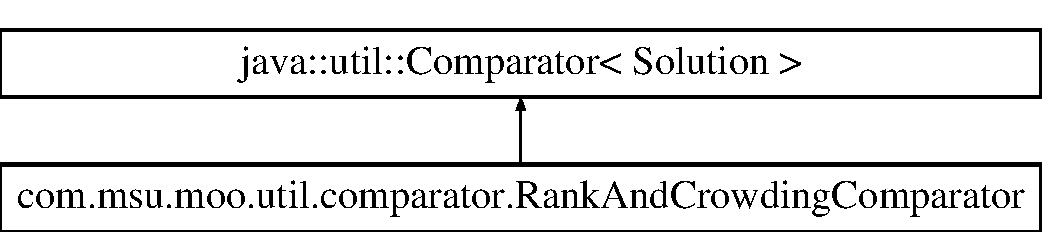
\includegraphics[height=2.000000cm]{classcom_1_1msu_1_1moo_1_1util_1_1comparator_1_1RankAndCrowdingComparator}
\end{center}
\end{figure}
\subsection*{Public Member Functions}
\begin{DoxyCompactItemize}
\item 
\hypertarget{classcom_1_1msu_1_1moo_1_1util_1_1comparator_1_1RankAndCrowdingComparator_a6f5153980f8ef6b4351ac043a13e42ff}{{\bfseries Rank\-And\-Crowding\-Comparator} (Map$<$ \hyperlink{classcom_1_1msu_1_1moo_1_1model_1_1solution_1_1Solution}{Solution}, Integer $>$ rank, Map$<$ \hyperlink{classcom_1_1msu_1_1moo_1_1model_1_1solution_1_1Solution}{Solution}, Double $>$ crowding)}\label{classcom_1_1msu_1_1moo_1_1util_1_1comparator_1_1RankAndCrowdingComparator_a6f5153980f8ef6b4351ac043a13e42ff}

\item 
\hypertarget{classcom_1_1msu_1_1moo_1_1util_1_1comparator_1_1RankAndCrowdingComparator_a78325edd99ed2af6ed2174413d36e162}{int {\bfseries compare} (\hyperlink{classcom_1_1msu_1_1moo_1_1model_1_1solution_1_1Solution}{Solution} o1, \hyperlink{classcom_1_1msu_1_1moo_1_1model_1_1solution_1_1Solution}{Solution} o2)}\label{classcom_1_1msu_1_1moo_1_1util_1_1comparator_1_1RankAndCrowdingComparator_a78325edd99ed2af6ed2174413d36e162}

\end{DoxyCompactItemize}
\subsection*{Protected Attributes}
\begin{DoxyCompactItemize}
\item 
\hypertarget{classcom_1_1msu_1_1moo_1_1util_1_1comparator_1_1RankAndCrowdingComparator_a1c755c06b7e2fbb5c291104be31241ed}{Map$<$ \hyperlink{classcom_1_1msu_1_1moo_1_1model_1_1solution_1_1Solution}{Solution}, Integer $>$ {\bfseries rank}}\label{classcom_1_1msu_1_1moo_1_1util_1_1comparator_1_1RankAndCrowdingComparator_a1c755c06b7e2fbb5c291104be31241ed}

\item 
\hypertarget{classcom_1_1msu_1_1moo_1_1util_1_1comparator_1_1RankAndCrowdingComparator_a313221f41fa182076e22e6ea3f884b76}{Map$<$ \hyperlink{classcom_1_1msu_1_1moo_1_1model_1_1solution_1_1Solution}{Solution}, Double $>$ {\bfseries crowding}}\label{classcom_1_1msu_1_1moo_1_1util_1_1comparator_1_1RankAndCrowdingComparator_a313221f41fa182076e22e6ea3f884b76}

\end{DoxyCompactItemize}


The documentation for this class was generated from the following file\-:\begin{DoxyCompactItemize}
\item 
src/main/java/com/msu/moo/util/comparator/Rank\-And\-Crowding\-Comparator.\-java\end{DoxyCompactItemize}

\hypertarget{classcom_1_1msu_1_1moo_1_1operators_1_1mutation_1_1RealMutation}{\section{com.\-msu.\-moo.\-operators.\-mutation.\-Real\-Mutation Class Reference}
\label{classcom_1_1msu_1_1moo_1_1operators_1_1mutation_1_1RealMutation}\index{com.\-msu.\-moo.\-operators.\-mutation.\-Real\-Mutation@{com.\-msu.\-moo.\-operators.\-mutation.\-Real\-Mutation}}
}
Inheritance diagram for com.\-msu.\-moo.\-operators.\-mutation.\-Real\-Mutation\-:\begin{figure}[H]
\begin{center}
\leavevmode
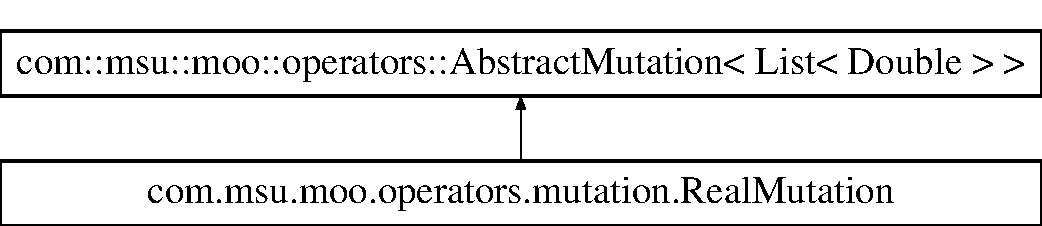
\includegraphics[height=2.000000cm]{classcom_1_1msu_1_1moo_1_1operators_1_1mutation_1_1RealMutation}
\end{center}
\end{figure}
\subsection*{Public Member Functions}
\begin{DoxyCompactItemize}
\item 
\hyperlink{classcom_1_1msu_1_1moo_1_1operators_1_1mutation_1_1RealMutation_a18bba16fa64c7035f702aa45b79fc9d5}{Real\-Mutation} ()
\item 
\hypertarget{classcom_1_1msu_1_1moo_1_1operators_1_1mutation_1_1RealMutation_abac684c5f72a41d9f57c6af409445717}{{\bfseries Real\-Mutation} (Double\mbox{[}$\,$\mbox{]} range)}\label{classcom_1_1msu_1_1moo_1_1operators_1_1mutation_1_1RealMutation_abac684c5f72a41d9f57c6af409445717}

\item 
\hypertarget{classcom_1_1msu_1_1moo_1_1operators_1_1mutation_1_1RealMutation_a507a1e592293383795ba61f0bd9e416a}{void {\bfseries set\-Range} (Double\mbox{[}$\,$\mbox{]} range)}\label{classcom_1_1msu_1_1moo_1_1operators_1_1mutation_1_1RealMutation_a507a1e592293383795ba61f0bd9e416a}

\end{DoxyCompactItemize}
\subsection*{Protected Member Functions}
\begin{DoxyCompactItemize}
\item 
\hypertarget{classcom_1_1msu_1_1moo_1_1operators_1_1mutation_1_1RealMutation_ab8d3fd3eed25e69ce58c55abc5919ed1}{Double {\bfseries sbx\-Mutation} (double p, double lower\-Bound, double upper\-Bound)}\label{classcom_1_1msu_1_1moo_1_1operators_1_1mutation_1_1RealMutation_ab8d3fd3eed25e69ce58c55abc5919ed1}

\item 
\hypertarget{classcom_1_1msu_1_1moo_1_1operators_1_1mutation_1_1RealMutation_a903b6389a21a1804977983a006b8281f}{void {\bfseries mutate\-\_\-} (List$<$ Double $>$ b)}\label{classcom_1_1msu_1_1moo_1_1operators_1_1mutation_1_1RealMutation_a903b6389a21a1804977983a006b8281f}

\end{DoxyCompactItemize}
\subsection*{Protected Attributes}
\begin{DoxyCompactItemize}
\item 
\hypertarget{classcom_1_1msu_1_1moo_1_1operators_1_1mutation_1_1RealMutation_a94d80dbe78bc9cc04669c0b7291017a0}{Double {\bfseries m\-Probability} = null}\label{classcom_1_1msu_1_1moo_1_1operators_1_1mutation_1_1RealMutation_a94d80dbe78bc9cc04669c0b7291017a0}

\item 
\hypertarget{classcom_1_1msu_1_1moo_1_1operators_1_1mutation_1_1RealMutation_a4fc25fa76dc66e075085a391a3d239fc}{Double\mbox{[}$\,$\mbox{]} {\bfseries range} = new Double\mbox{[}$\,$\mbox{]} \{ Double.\-M\-I\-N\-\_\-\-V\-A\-L\-U\-E, Double.\-M\-A\-X\-\_\-\-V\-A\-L\-U\-E \}}\label{classcom_1_1msu_1_1moo_1_1operators_1_1mutation_1_1RealMutation_a4fc25fa76dc66e075085a391a3d239fc}

\item 
\hypertarget{classcom_1_1msu_1_1moo_1_1operators_1_1mutation_1_1RealMutation_ab6364b111e32f84e04360375bc1adeff}{double \hyperlink{classcom_1_1msu_1_1moo_1_1operators_1_1mutation_1_1RealMutation_ab6364b111e32f84e04360375bc1adeff}{eta\-\_\-m} = 20.\-0}\label{classcom_1_1msu_1_1moo_1_1operators_1_1mutation_1_1RealMutation_ab6364b111e32f84e04360375bc1adeff}

\begin{DoxyCompactList}\small\item\em distribution index \end{DoxyCompactList}\item 
\hypertarget{classcom_1_1msu_1_1moo_1_1operators_1_1mutation_1_1RealMutation_ae0bad9fd2250042497a349e4f9b7de85}{\hyperlink{classcom_1_1msu_1_1moo_1_1util_1_1Random}{Random} {\bfseries r} = \hyperlink{classcom_1_1msu_1_1moo_1_1util_1_1Random_aaa20005ec38b5944262c79c06d92ab62}{Random.\-get\-Instance}()}\label{classcom_1_1msu_1_1moo_1_1operators_1_1mutation_1_1RealMutation_ae0bad9fd2250042497a349e4f9b7de85}

\end{DoxyCompactItemize}


\subsection{Constructor \& Destructor Documentation}
\hypertarget{classcom_1_1msu_1_1moo_1_1operators_1_1mutation_1_1RealMutation_a18bba16fa64c7035f702aa45b79fc9d5}{\index{com\-::msu\-::moo\-::operators\-::mutation\-::\-Real\-Mutation@{com\-::msu\-::moo\-::operators\-::mutation\-::\-Real\-Mutation}!Real\-Mutation@{Real\-Mutation}}
\index{Real\-Mutation@{Real\-Mutation}!com::msu::moo::operators::mutation::RealMutation@{com\-::msu\-::moo\-::operators\-::mutation\-::\-Real\-Mutation}}
\subsubsection[{Real\-Mutation}]{\setlength{\rightskip}{0pt plus 5cm}com.\-msu.\-moo.\-operators.\-mutation.\-Real\-Mutation.\-Real\-Mutation (
\begin{DoxyParamCaption}
{}
\end{DoxyParamCaption}
)\hspace{0.3cm}{\ttfamily [inline]}}}\label{classcom_1_1msu_1_1moo_1_1operators_1_1mutation_1_1RealMutation_a18bba16fa64c7035f702aa45b79fc9d5}
Normal constructor with dynamic probability 

The documentation for this class was generated from the following file\-:\begin{DoxyCompactItemize}
\item 
src/main/java/com/msu/moo/operators/mutation/Real\-Mutation.\-java\end{DoxyCompactItemize}

\hypertarget{classcom_1_1msu_1_1moo_1_1operators_1_1mutation_1_1RestrictedPolynomialMutation}{\section{com.\-msu.\-moo.\-operators.\-mutation.\-Restricted\-Polynomial\-Mutation Class Reference}
\label{classcom_1_1msu_1_1moo_1_1operators_1_1mutation_1_1RestrictedPolynomialMutation}\index{com.\-msu.\-moo.\-operators.\-mutation.\-Restricted\-Polynomial\-Mutation@{com.\-msu.\-moo.\-operators.\-mutation.\-Restricted\-Polynomial\-Mutation}}
}
Inheritance diagram for com.\-msu.\-moo.\-operators.\-mutation.\-Restricted\-Polynomial\-Mutation\-:\begin{figure}[H]
\begin{center}
\leavevmode
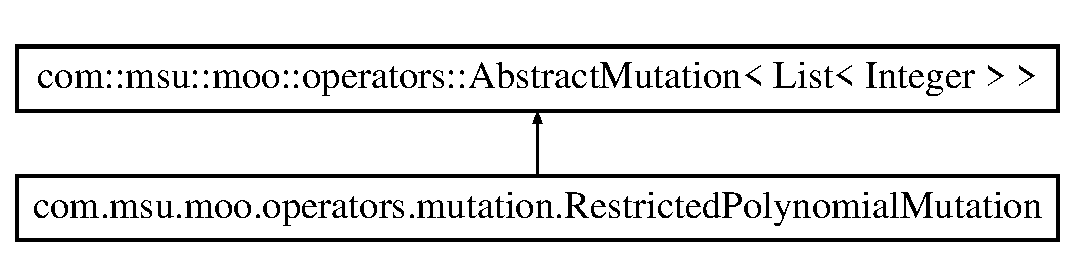
\includegraphics[height=2.000000cm]{classcom_1_1msu_1_1moo_1_1operators_1_1mutation_1_1RestrictedPolynomialMutation}
\end{center}
\end{figure}
\subsection*{Public Member Functions}
\begin{DoxyCompactItemize}
\item 
\hyperlink{classcom_1_1msu_1_1moo_1_1operators_1_1mutation_1_1RestrictedPolynomialMutation_ae9864b40662ace354ddbd9e64679ab81}{Restricted\-Polynomial\-Mutation} ()
\item 
\hyperlink{classcom_1_1msu_1_1moo_1_1operators_1_1mutation_1_1RestrictedPolynomialMutation_ae9be3ac0bef17c893da91a5022394332}{Restricted\-Polynomial\-Mutation} (Double \hyperlink{classcom_1_1msu_1_1moo_1_1operators_1_1mutation_1_1RestrictedPolynomialMutation_a1f8ad0e089b42b3641b6e79ae6a5fcba}{probability})
\end{DoxyCompactItemize}
\subsection*{Protected Member Functions}
\begin{DoxyCompactItemize}
\item 
\hypertarget{classcom_1_1msu_1_1moo_1_1operators_1_1mutation_1_1RestrictedPolynomialMutation_af8c71ae956c098bafc7c55887af940f0}{void {\bfseries mutate\-\_\-} (List$<$ Integer $>$ b)}\label{classcom_1_1msu_1_1moo_1_1operators_1_1mutation_1_1RestrictedPolynomialMutation_af8c71ae956c098bafc7c55887af940f0}

\end{DoxyCompactItemize}
\subsection*{Protected Attributes}
\begin{DoxyCompactItemize}
\item 
\hypertarget{classcom_1_1msu_1_1moo_1_1operators_1_1mutation_1_1RestrictedPolynomialMutation_a1f8ad0e089b42b3641b6e79ae6a5fcba}{Double \hyperlink{classcom_1_1msu_1_1moo_1_1operators_1_1mutation_1_1RestrictedPolynomialMutation_a1f8ad0e089b42b3641b6e79ae6a5fcba}{probability} = null}\label{classcom_1_1msu_1_1moo_1_1operators_1_1mutation_1_1RestrictedPolynomialMutation_a1f8ad0e089b42b3641b6e79ae6a5fcba}

\begin{DoxyCompactList}\small\item\em the probability that a bit is changed \end{DoxyCompactList}\end{DoxyCompactItemize}


\subsection{Detailed Description}
This is a basic \hyperlink{classcom_1_1msu_1_1moo_1_1operators_1_1mutation_1_1BitFlipMutation}{Bit\-Flip\-Mutation} which is allowed on all List$<$\-Boolean$>$ objects. There are two objects\-: there could be a fix probability or it is 1/length of object.

\mbox{[}0,0,1,0\mbox{]} -\/---$>$ \mbox{[}1,0,1,0\mbox{]} 

\subsection{Constructor \& Destructor Documentation}
\hypertarget{classcom_1_1msu_1_1moo_1_1operators_1_1mutation_1_1RestrictedPolynomialMutation_ae9864b40662ace354ddbd9e64679ab81}{\index{com\-::msu\-::moo\-::operators\-::mutation\-::\-Restricted\-Polynomial\-Mutation@{com\-::msu\-::moo\-::operators\-::mutation\-::\-Restricted\-Polynomial\-Mutation}!Restricted\-Polynomial\-Mutation@{Restricted\-Polynomial\-Mutation}}
\index{Restricted\-Polynomial\-Mutation@{Restricted\-Polynomial\-Mutation}!com::msu::moo::operators::mutation::RestrictedPolynomialMutation@{com\-::msu\-::moo\-::operators\-::mutation\-::\-Restricted\-Polynomial\-Mutation}}
\subsubsection[{Restricted\-Polynomial\-Mutation}]{\setlength{\rightskip}{0pt plus 5cm}com.\-msu.\-moo.\-operators.\-mutation.\-Restricted\-Polynomial\-Mutation.\-Restricted\-Polynomial\-Mutation (
\begin{DoxyParamCaption}
{}
\end{DoxyParamCaption}
)\hspace{0.3cm}{\ttfamily [inline]}}}\label{classcom_1_1msu_1_1moo_1_1operators_1_1mutation_1_1RestrictedPolynomialMutation_ae9864b40662ace354ddbd9e64679ab81}
Normal constructor with dynamic probability \hypertarget{classcom_1_1msu_1_1moo_1_1operators_1_1mutation_1_1RestrictedPolynomialMutation_ae9be3ac0bef17c893da91a5022394332}{\index{com\-::msu\-::moo\-::operators\-::mutation\-::\-Restricted\-Polynomial\-Mutation@{com\-::msu\-::moo\-::operators\-::mutation\-::\-Restricted\-Polynomial\-Mutation}!Restricted\-Polynomial\-Mutation@{Restricted\-Polynomial\-Mutation}}
\index{Restricted\-Polynomial\-Mutation@{Restricted\-Polynomial\-Mutation}!com::msu::moo::operators::mutation::RestrictedPolynomialMutation@{com\-::msu\-::moo\-::operators\-::mutation\-::\-Restricted\-Polynomial\-Mutation}}
\subsubsection[{Restricted\-Polynomial\-Mutation}]{\setlength{\rightskip}{0pt plus 5cm}com.\-msu.\-moo.\-operators.\-mutation.\-Restricted\-Polynomial\-Mutation.\-Restricted\-Polynomial\-Mutation (
\begin{DoxyParamCaption}
\item[{Double}]{probability}
\end{DoxyParamCaption}
)\hspace{0.3cm}{\ttfamily [inline]}}}\label{classcom_1_1msu_1_1moo_1_1operators_1_1mutation_1_1RestrictedPolynomialMutation_ae9be3ac0bef17c893da91a5022394332}
Constructor which fixes the probability for all inputs. 
\begin{DoxyParams}{Parameters}
{\em probability} & that a bit is changed \\
\hline
\end{DoxyParams}


The documentation for this class was generated from the following file\-:\begin{DoxyCompactItemize}
\item 
src/main/java/com/msu/moo/operators/mutation/Restricted\-Polynomial\-Mutation.\-java\end{DoxyCompactItemize}

\hypertarget{classcom_1_1msu_1_1moo_1_1visualization_1_1ScatterPlot}{\section{com.\-msu.\-moo.\-visualization.\-Scatter\-Plot Class Reference}
\label{classcom_1_1msu_1_1moo_1_1visualization_1_1ScatterPlot}\index{com.\-msu.\-moo.\-visualization.\-Scatter\-Plot@{com.\-msu.\-moo.\-visualization.\-Scatter\-Plot}}
}
Inheritance diagram for com.\-msu.\-moo.\-visualization.\-Scatter\-Plot\-:\begin{figure}[H]
\begin{center}
\leavevmode
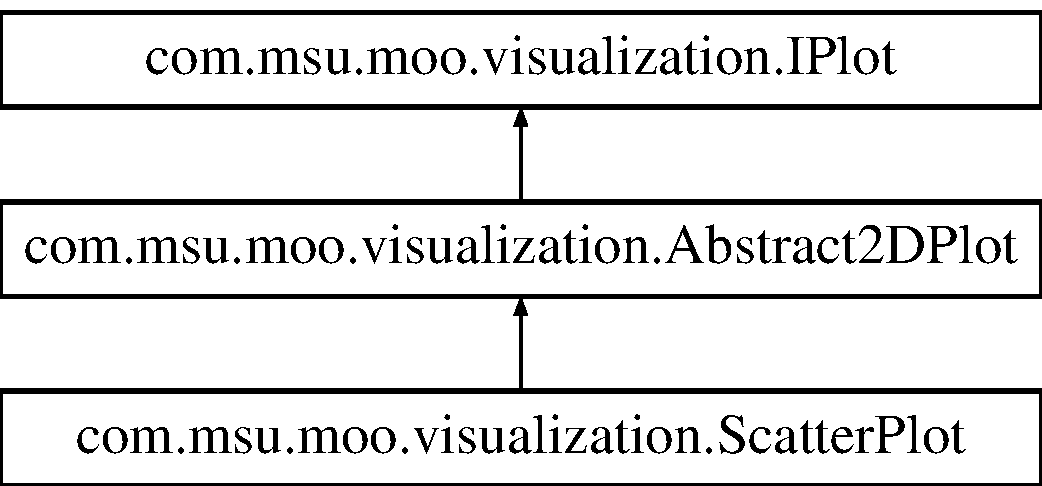
\includegraphics[height=3.000000cm]{classcom_1_1msu_1_1moo_1_1visualization_1_1ScatterPlot}
\end{center}
\end{figure}
\subsection*{Public Member Functions}
\begin{DoxyCompactItemize}
\item 
\hypertarget{classcom_1_1msu_1_1moo_1_1visualization_1_1ScatterPlot_ae1641035e865ac60aa17ec5be881fdf6}{{\bfseries Scatter\-Plot} (String title)}\label{classcom_1_1msu_1_1moo_1_1visualization_1_1ScatterPlot_ae1641035e865ac60aa17ec5be881fdf6}

\item 
\hypertarget{classcom_1_1msu_1_1moo_1_1visualization_1_1ScatterPlot_ad4155b5893e37944768a35b90ede23e4}{{\bfseries Scatter\-Plot} (String title, String x\-Label, String y\-Label)}\label{classcom_1_1msu_1_1moo_1_1visualization_1_1ScatterPlot_ad4155b5893e37944768a35b90ede23e4}

\item 
void \hyperlink{classcom_1_1msu_1_1moo_1_1visualization_1_1ScatterPlot_abf7740669f9017367f5ac05899179854}{add} (\hyperlink{classcom_1_1msu_1_1moo_1_1model_1_1solution_1_1SolutionSet}{Solution\-Set} set, String name)
\item 
\hypertarget{classcom_1_1msu_1_1moo_1_1visualization_1_1ScatterPlot_a00d6f928daa34c96950eb780c8bff4b8}{void {\bfseries add} (\hyperlink{classcom_1_1msu_1_1moo_1_1model_1_1solution_1_1NonDominatedSolutionSet}{Non\-Dominated\-Solution\-Set} set, String name)}\label{classcom_1_1msu_1_1moo_1_1visualization_1_1ScatterPlot_a00d6f928daa34c96950eb780c8bff4b8}

\item 
J\-Free\-Chart \hyperlink{classcom_1_1msu_1_1moo_1_1visualization_1_1ScatterPlot_a1c5117bd94b91e9ae2f59c1c025b243b}{get\-Chart} ()
\end{DoxyCompactItemize}
\subsection*{Protected Attributes}
\begin{DoxyCompactItemize}
\item 
\hypertarget{classcom_1_1msu_1_1moo_1_1visualization_1_1ScatterPlot_aa1dbce1c6b6c7a1a98eca2df5f871d44}{X\-Y\-Series\-Collection {\bfseries collection} = new X\-Y\-Series\-Collection()}\label{classcom_1_1msu_1_1moo_1_1visualization_1_1ScatterPlot_aa1dbce1c6b6c7a1a98eca2df5f871d44}

\end{DoxyCompactItemize}


\subsection{Member Function Documentation}
\hypertarget{classcom_1_1msu_1_1moo_1_1visualization_1_1ScatterPlot_abf7740669f9017367f5ac05899179854}{\index{com\-::msu\-::moo\-::visualization\-::\-Scatter\-Plot@{com\-::msu\-::moo\-::visualization\-::\-Scatter\-Plot}!add@{add}}
\index{add@{add}!com::msu::moo::visualization::ScatterPlot@{com\-::msu\-::moo\-::visualization\-::\-Scatter\-Plot}}
\subsubsection[{add}]{\setlength{\rightskip}{0pt plus 5cm}void com.\-msu.\-moo.\-visualization.\-Scatter\-Plot.\-add (
\begin{DoxyParamCaption}
\item[{{\bf Solution\-Set}}]{set, }
\item[{String}]{name}
\end{DoxyParamCaption}
)\hspace{0.3cm}{\ttfamily [inline]}}}\label{classcom_1_1msu_1_1moo_1_1visualization_1_1ScatterPlot_abf7740669f9017367f5ac05899179854}
Add a solution set to scatter plot! 
\begin{DoxyParams}{Parameters}
{\em set} & with the data points. Must be 2\-D in objective space!! \\
\hline
{\em name} & of the data set \\
\hline
\end{DoxyParams}
\hypertarget{classcom_1_1msu_1_1moo_1_1visualization_1_1ScatterPlot_a1c5117bd94b91e9ae2f59c1c025b243b}{\index{com\-::msu\-::moo\-::visualization\-::\-Scatter\-Plot@{com\-::msu\-::moo\-::visualization\-::\-Scatter\-Plot}!get\-Chart@{get\-Chart}}
\index{get\-Chart@{get\-Chart}!com::msu::moo::visualization::ScatterPlot@{com\-::msu\-::moo\-::visualization\-::\-Scatter\-Plot}}
\subsubsection[{get\-Chart}]{\setlength{\rightskip}{0pt plus 5cm}J\-Free\-Chart com.\-msu.\-moo.\-visualization.\-Scatter\-Plot.\-get\-Chart (
\begin{DoxyParamCaption}
{}
\end{DoxyParamCaption}
)\hspace{0.3cm}{\ttfamily [inline]}}}\label{classcom_1_1msu_1_1moo_1_1visualization_1_1ScatterPlot_a1c5117bd94b91e9ae2f59c1c025b243b}
Every Plot needs the chart frame to visualize the results \begin{DoxyReturn}{Returns}
chart frame to make it visible 
\end{DoxyReturn}


Implements \hyperlink{interfacecom_1_1msu_1_1moo_1_1visualization_1_1IPlot_ae45c2987d112fbf5bc5af7864fb50ecd}{com.\-msu.\-moo.\-visualization.\-I\-Plot}.



The documentation for this class was generated from the following file\-:\begin{DoxyCompactItemize}
\item 
src/main/java/com/msu/moo/visualization/Scatter\-Plot.\-java\end{DoxyCompactItemize}

\hypertarget{classcom_1_1msu_1_1moo_1_1operators_1_1crossover_1_1SimulatedBinaryCrossover}{\section{com.\-msu.\-moo.\-operators.\-crossover.\-Simulated\-Binary\-Crossover Class Reference}
\label{classcom_1_1msu_1_1moo_1_1operators_1_1crossover_1_1SimulatedBinaryCrossover}\index{com.\-msu.\-moo.\-operators.\-crossover.\-Simulated\-Binary\-Crossover@{com.\-msu.\-moo.\-operators.\-crossover.\-Simulated\-Binary\-Crossover}}
}
Inheritance diagram for com.\-msu.\-moo.\-operators.\-crossover.\-Simulated\-Binary\-Crossover\-:\begin{figure}[H]
\begin{center}
\leavevmode
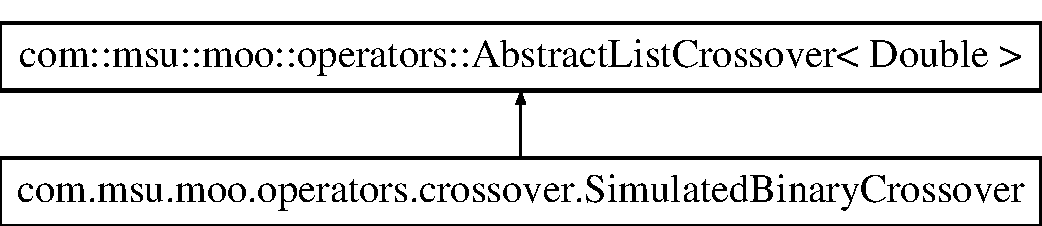
\includegraphics[height=2.000000cm]{classcom_1_1msu_1_1moo_1_1operators_1_1crossover_1_1SimulatedBinaryCrossover}
\end{center}
\end{figure}
\subsection*{Public Member Functions}
\begin{DoxyCompactItemize}
\item 
\hypertarget{classcom_1_1msu_1_1moo_1_1operators_1_1crossover_1_1SimulatedBinaryCrossover_ac53a622aa37bb4b1f600c48c5dec2b1c}{{\bfseries Simulated\-Binary\-Crossover} (double\mbox{[}$\,$\mbox{]} range)}\label{classcom_1_1msu_1_1moo_1_1operators_1_1crossover_1_1SimulatedBinaryCrossover_ac53a622aa37bb4b1f600c48c5dec2b1c}

\end{DoxyCompactItemize}
\subsection*{Protected Member Functions}
\begin{DoxyCompactItemize}
\item 
double \hyperlink{classcom_1_1msu_1_1moo_1_1operators_1_1crossover_1_1SimulatedBinaryCrossover_aae397584c8051c4d1fc84f188a706e37}{calc\-Beta} (double u, double alpha, double \hyperlink{classcom_1_1msu_1_1moo_1_1operators_1_1crossover_1_1SimulatedBinaryCrossover_af0cddf432a1f07e77a59a334caa267d2}{eta\-\_\-c})
\item 
double \hyperlink{classcom_1_1msu_1_1moo_1_1operators_1_1crossover_1_1SimulatedBinaryCrossover_ac584dfe83a0ecfedc90fdb574760b2c7}{calc\-Aplha\-Lower} (double p1, double p2, double lower\-Bound)
\item 
double \hyperlink{classcom_1_1msu_1_1moo_1_1operators_1_1crossover_1_1SimulatedBinaryCrossover_a2630f64686cc61c89549d25735715c68}{calc\-Aplha\-Upper} (double p1, double p2, double upper\-Bound)
\item 
Pair$<$ Double, Double $>$ \hyperlink{classcom_1_1msu_1_1moo_1_1operators_1_1crossover_1_1SimulatedBinaryCrossover_a37fd1bc12cb37b3171e84c9a9b190819}{S\-B\-X} (double d1, double d2, double lower\-Bound, double upper\-Bound)
\item 
\hypertarget{classcom_1_1msu_1_1moo_1_1operators_1_1crossover_1_1SimulatedBinaryCrossover_a958facba6c422920e7e87b46e671de92}{List$<$ List$<$ Double $>$ $>$ {\bfseries crossover\-Lists} (List$<$ Double $>$ parent1, List$<$ Double $>$ parent2)}\label{classcom_1_1msu_1_1moo_1_1operators_1_1crossover_1_1SimulatedBinaryCrossover_a958facba6c422920e7e87b46e671de92}

\end{DoxyCompactItemize}
\subsection*{Protected Attributes}
\begin{DoxyCompactItemize}
\item 
\hypertarget{classcom_1_1msu_1_1moo_1_1operators_1_1crossover_1_1SimulatedBinaryCrossover_a6e8b9e99a9971880417c88e3f9e9cea5}{double {\bfseries E\-P\-S} = 1.\-0e-\/30}\label{classcom_1_1msu_1_1moo_1_1operators_1_1crossover_1_1SimulatedBinaryCrossover_a6e8b9e99a9971880417c88e3f9e9cea5}

\item 
\hypertarget{classcom_1_1msu_1_1moo_1_1operators_1_1crossover_1_1SimulatedBinaryCrossover_a4553b6d3c2b8cbc549e490fbc3a45323}{double\mbox{[}$\,$\mbox{]} {\bfseries range} = new double\mbox{[}$\,$\mbox{]} \{ Double.\-M\-I\-N\-\_\-\-V\-A\-L\-U\-E, Double.\-M\-A\-X\-\_\-\-V\-A\-L\-U\-E \}}\label{classcom_1_1msu_1_1moo_1_1operators_1_1crossover_1_1SimulatedBinaryCrossover_a4553b6d3c2b8cbc549e490fbc3a45323}

\item 
\hypertarget{classcom_1_1msu_1_1moo_1_1operators_1_1crossover_1_1SimulatedBinaryCrossover_af0cddf432a1f07e77a59a334caa267d2}{double \hyperlink{classcom_1_1msu_1_1moo_1_1operators_1_1crossover_1_1SimulatedBinaryCrossover_af0cddf432a1f07e77a59a334caa267d2}{eta\-\_\-c} = 20.\-0}\label{classcom_1_1msu_1_1moo_1_1operators_1_1crossover_1_1SimulatedBinaryCrossover_af0cddf432a1f07e77a59a334caa267d2}

\begin{DoxyCompactList}\small\item\em distribution index \end{DoxyCompactList}\item 
\hypertarget{classcom_1_1msu_1_1moo_1_1operators_1_1crossover_1_1SimulatedBinaryCrossover_ab9b946b17f8129fba3a742ac73429680}{double \hyperlink{classcom_1_1msu_1_1moo_1_1operators_1_1crossover_1_1SimulatedBinaryCrossover_ab9b946b17f8129fba3a742ac73429680}{c\-Probability} = 0.\-5}\label{classcom_1_1msu_1_1moo_1_1operators_1_1crossover_1_1SimulatedBinaryCrossover_ab9b946b17f8129fba3a742ac73429680}

\begin{DoxyCompactList}\small\item\em crossover probability in the list \end{DoxyCompactList}\item 
\hypertarget{classcom_1_1msu_1_1moo_1_1operators_1_1crossover_1_1SimulatedBinaryCrossover_a60baf5b10ddc7bf7fa827ff7dde954a5}{\hyperlink{classcom_1_1msu_1_1moo_1_1util_1_1Random}{Random} {\bfseries r} = \hyperlink{classcom_1_1msu_1_1moo_1_1util_1_1Random_aaa20005ec38b5944262c79c06d92ab62}{Random.\-get\-Instance}()}\label{classcom_1_1msu_1_1moo_1_1operators_1_1crossover_1_1SimulatedBinaryCrossover_a60baf5b10ddc7bf7fa827ff7dde954a5}

\end{DoxyCompactItemize}


\subsection{Member Function Documentation}
\hypertarget{classcom_1_1msu_1_1moo_1_1operators_1_1crossover_1_1SimulatedBinaryCrossover_ac584dfe83a0ecfedc90fdb574760b2c7}{\index{com\-::msu\-::moo\-::operators\-::crossover\-::\-Simulated\-Binary\-Crossover@{com\-::msu\-::moo\-::operators\-::crossover\-::\-Simulated\-Binary\-Crossover}!calc\-Aplha\-Lower@{calc\-Aplha\-Lower}}
\index{calc\-Aplha\-Lower@{calc\-Aplha\-Lower}!com::msu::moo::operators::crossover::SimulatedBinaryCrossover@{com\-::msu\-::moo\-::operators\-::crossover\-::\-Simulated\-Binary\-Crossover}}
\subsubsection[{calc\-Aplha\-Lower}]{\setlength{\rightskip}{0pt plus 5cm}double com.\-msu.\-moo.\-operators.\-crossover.\-Simulated\-Binary\-Crossover.\-calc\-Aplha\-Lower (
\begin{DoxyParamCaption}
\item[{double}]{p1, }
\item[{double}]{p2, }
\item[{double}]{lower\-Bound}
\end{DoxyParamCaption}
)\hspace{0.3cm}{\ttfamily [inline]}, {\ttfamily [protected]}}}\label{classcom_1_1msu_1_1moo_1_1operators_1_1crossover_1_1SimulatedBinaryCrossover_ac584dfe83a0ecfedc90fdb574760b2c7}
p1 $<$ p2 has to be true 
\begin{DoxyParams}{Parameters}
{\em p1} & first parent \\
\hline
{\em p2} & second parent \\
\hline
{\em lower\-Bound} & the lower bound which should hold for the child \\
\hline
\end{DoxyParams}
\begin{DoxyReturn}{Returns}
alpha value for the lower child 
\end{DoxyReturn}
\hypertarget{classcom_1_1msu_1_1moo_1_1operators_1_1crossover_1_1SimulatedBinaryCrossover_a2630f64686cc61c89549d25735715c68}{\index{com\-::msu\-::moo\-::operators\-::crossover\-::\-Simulated\-Binary\-Crossover@{com\-::msu\-::moo\-::operators\-::crossover\-::\-Simulated\-Binary\-Crossover}!calc\-Aplha\-Upper@{calc\-Aplha\-Upper}}
\index{calc\-Aplha\-Upper@{calc\-Aplha\-Upper}!com::msu::moo::operators::crossover::SimulatedBinaryCrossover@{com\-::msu\-::moo\-::operators\-::crossover\-::\-Simulated\-Binary\-Crossover}}
\subsubsection[{calc\-Aplha\-Upper}]{\setlength{\rightskip}{0pt plus 5cm}double com.\-msu.\-moo.\-operators.\-crossover.\-Simulated\-Binary\-Crossover.\-calc\-Aplha\-Upper (
\begin{DoxyParamCaption}
\item[{double}]{p1, }
\item[{double}]{p2, }
\item[{double}]{upper\-Bound}
\end{DoxyParamCaption}
)\hspace{0.3cm}{\ttfamily [inline]}, {\ttfamily [protected]}}}\label{classcom_1_1msu_1_1moo_1_1operators_1_1crossover_1_1SimulatedBinaryCrossover_a2630f64686cc61c89549d25735715c68}
p1 $<$ p2 has to be true \begin{DoxyReturn}{Returns}
alpha value for the upper child 
\end{DoxyReturn}
\hypertarget{classcom_1_1msu_1_1moo_1_1operators_1_1crossover_1_1SimulatedBinaryCrossover_aae397584c8051c4d1fc84f188a706e37}{\index{com\-::msu\-::moo\-::operators\-::crossover\-::\-Simulated\-Binary\-Crossover@{com\-::msu\-::moo\-::operators\-::crossover\-::\-Simulated\-Binary\-Crossover}!calc\-Beta@{calc\-Beta}}
\index{calc\-Beta@{calc\-Beta}!com::msu::moo::operators::crossover::SimulatedBinaryCrossover@{com\-::msu\-::moo\-::operators\-::crossover\-::\-Simulated\-Binary\-Crossover}}
\subsubsection[{calc\-Beta}]{\setlength{\rightskip}{0pt plus 5cm}double com.\-msu.\-moo.\-operators.\-crossover.\-Simulated\-Binary\-Crossover.\-calc\-Beta (
\begin{DoxyParamCaption}
\item[{double}]{u, }
\item[{double}]{alpha, }
\item[{double}]{eta\-\_\-c}
\end{DoxyParamCaption}
)\hspace{0.3cm}{\ttfamily [inline]}, {\ttfamily [protected]}}}\label{classcom_1_1msu_1_1moo_1_1operators_1_1crossover_1_1SimulatedBinaryCrossover_aae397584c8051c4d1fc84f188a706e37}
Calculate like


\begin{DoxyParams}{Parameters}
{\em u} & random variable between \mbox{[}0,1\mbox{]} \\
\hline
{\em alpha} & \\
\hline
\end{DoxyParams}
\begin{DoxyReturn}{Returns}
beta value 
\end{DoxyReturn}
\hypertarget{classcom_1_1msu_1_1moo_1_1operators_1_1crossover_1_1SimulatedBinaryCrossover_a37fd1bc12cb37b3171e84c9a9b190819}{\index{com\-::msu\-::moo\-::operators\-::crossover\-::\-Simulated\-Binary\-Crossover@{com\-::msu\-::moo\-::operators\-::crossover\-::\-Simulated\-Binary\-Crossover}!S\-B\-X@{S\-B\-X}}
\index{S\-B\-X@{S\-B\-X}!com::msu::moo::operators::crossover::SimulatedBinaryCrossover@{com\-::msu\-::moo\-::operators\-::crossover\-::\-Simulated\-Binary\-Crossover}}
\subsubsection[{S\-B\-X}]{\setlength{\rightskip}{0pt plus 5cm}Pair$<$Double, Double$>$ com.\-msu.\-moo.\-operators.\-crossover.\-Simulated\-Binary\-Crossover.\-S\-B\-X (
\begin{DoxyParamCaption}
\item[{double}]{d1, }
\item[{double}]{d2, }
\item[{double}]{lower\-Bound, }
\item[{double}]{upper\-Bound}
\end{DoxyParamCaption}
)\hspace{0.3cm}{\ttfamily [inline]}, {\ttfamily [protected]}}}\label{classcom_1_1msu_1_1moo_1_1operators_1_1crossover_1_1SimulatedBinaryCrossover_a37fd1bc12cb37b3171e84c9a9b190819}
S\-B\-X for two double variables \begin{DoxyReturn}{Returns}
offspring values which are in \mbox{[}lower\-Bound,upper\-Bound\mbox{]} 
\end{DoxyReturn}


The documentation for this class was generated from the following file\-:\begin{DoxyCompactItemize}
\item 
src/main/java/com/msu/moo/operators/crossover/Simulated\-Binary\-Crossover.\-java\end{DoxyCompactItemize}

\hypertarget{classcom_1_1msu_1_1moo_1_1operators_1_1crossover_1_1SinglePointCrossover_3_01T_01_4}{\section{com.\-msu.\-moo.\-operators.\-crossover.\-Single\-Point\-Crossover$<$ T $>$ Class Reference}
\label{classcom_1_1msu_1_1moo_1_1operators_1_1crossover_1_1SinglePointCrossover_3_01T_01_4}\index{com.\-msu.\-moo.\-operators.\-crossover.\-Single\-Point\-Crossover$<$ T $>$@{com.\-msu.\-moo.\-operators.\-crossover.\-Single\-Point\-Crossover$<$ T $>$}}
}
Inheritance diagram for com.\-msu.\-moo.\-operators.\-crossover.\-Single\-Point\-Crossover$<$ T $>$\-:\begin{figure}[H]
\begin{center}
\leavevmode
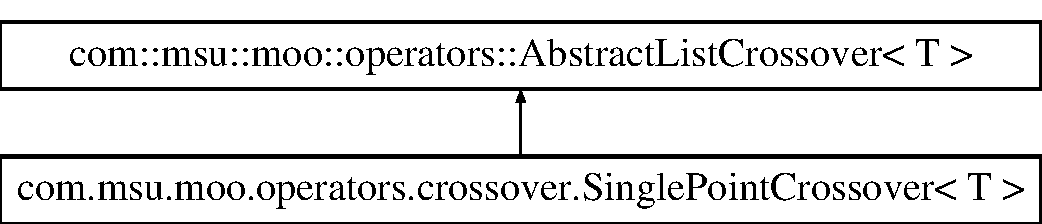
\includegraphics[height=2.000000cm]{classcom_1_1msu_1_1moo_1_1operators_1_1crossover_1_1SinglePointCrossover_3_01T_01_4}
\end{center}
\end{figure}
\subsection*{Protected Member Functions}
\begin{DoxyCompactItemize}
\item 
\hypertarget{classcom_1_1msu_1_1moo_1_1operators_1_1crossover_1_1SinglePointCrossover_3_01T_01_4_ad3b2c7c7e131d6f25060fb6b35d9464a}{List$<$ List$<$ T $>$ $>$ {\bfseries crossover\-\_\-} (List$<$ T $>$ a, List$<$ T $>$ b, int point)}\label{classcom_1_1msu_1_1moo_1_1operators_1_1crossover_1_1SinglePointCrossover_3_01T_01_4_ad3b2c7c7e131d6f25060fb6b35d9464a}

\item 
\hypertarget{classcom_1_1msu_1_1moo_1_1operators_1_1crossover_1_1SinglePointCrossover_3_01T_01_4_abcf803e3fa69e6bdb37c16a4f1c4acba}{List$<$ List$<$ T $>$ $>$ {\bfseries crossover\-Lists} (List$<$ T $>$ a, List$<$ T $>$ b)}\label{classcom_1_1msu_1_1moo_1_1operators_1_1crossover_1_1SinglePointCrossover_3_01T_01_4_abcf803e3fa69e6bdb37c16a4f1c4acba}

\end{DoxyCompactItemize}


\subsection{Detailed Description}
This is the single point crossover where a list with any type could but cut in a half and recombined with another half.

\mbox{[}0,1,2,3,4\mbox{]} and \mbox{[}4,3,2,1,0\mbox{]} and point is one leads to

\mbox{[}0\mbox{]} + \mbox{[}3,2,1,0\mbox{]} = \mbox{[}0,3,2,1,0\mbox{]} and \mbox{[}4\mbox{]} + \mbox{[}1,2,3,4\mbox{]} = \mbox{[}4,1,2,3,4\mbox{]} 

The documentation for this class was generated from the following file\-:\begin{DoxyCompactItemize}
\item 
src/main/java/com/msu/moo/operators/crossover/Single\-Point\-Crossover.\-java\end{DoxyCompactItemize}

\hypertarget{classcom_1_1msu_1_1moo_1_1model_1_1solution_1_1Solution}{\section{com.\-msu.\-moo.\-model.\-solution.\-Solution Class Reference}
\label{classcom_1_1msu_1_1moo_1_1model_1_1solution_1_1Solution}\index{com.\-msu.\-moo.\-model.\-solution.\-Solution@{com.\-msu.\-moo.\-model.\-solution.\-Solution}}
}
\subsection*{Public Member Functions}
\begin{DoxyCompactItemize}
\item 
\hyperlink{classcom_1_1msu_1_1moo_1_1model_1_1solution_1_1Solution_a759abac5dda1b043f5b0e6eda2326fc9}{Solution} (\hyperlink{interfacecom_1_1msu_1_1moo_1_1model_1_1interfaces_1_1IVariable}{I\-Variable} variable, List$<$ Double $>$ objectives)
\item 
List$<$ Double $>$ \hyperlink{classcom_1_1msu_1_1moo_1_1model_1_1solution_1_1Solution_a82ad1dc142a62508d5c18dd17d3eaf1c}{get\-Objectives} ()
\item 
\hyperlink{interfacecom_1_1msu_1_1moo_1_1model_1_1interfaces_1_1IVariable}{I\-Variable} \hyperlink{classcom_1_1msu_1_1moo_1_1model_1_1solution_1_1Solution_ad5bb8160a7db2be6a161683362a13e33}{get\-Variable} ()
\item 
\hypertarget{classcom_1_1msu_1_1moo_1_1model_1_1solution_1_1Solution_a72a3ed4642fd006574ed1790464cfc53}{int {\bfseries count\-Objectives} ()}\label{classcom_1_1msu_1_1moo_1_1model_1_1solution_1_1Solution_a72a3ed4642fd006574ed1790464cfc53}

\item 
String \hyperlink{classcom_1_1msu_1_1moo_1_1model_1_1solution_1_1Solution_a4e9941d11c66d5bf0288c867540b1b19}{to\-String} ()
\end{DoxyCompactItemize}


\subsection{Detailed Description}
This class combines the variable with the result in the objective space. Each instance is I\-M\-M\-U\-T\-A\-B\-L\-E which means a solution that is calculate could not be altered anymore.

This concept ensure to forget to reevaluate a solution which means result and variables does not fit anymore. 

\subsection{Constructor \& Destructor Documentation}
\hypertarget{classcom_1_1msu_1_1moo_1_1model_1_1solution_1_1Solution_a759abac5dda1b043f5b0e6eda2326fc9}{\index{com\-::msu\-::moo\-::model\-::solution\-::\-Solution@{com\-::msu\-::moo\-::model\-::solution\-::\-Solution}!Solution@{Solution}}
\index{Solution@{Solution}!com::msu::moo::model::solution::Solution@{com\-::msu\-::moo\-::model\-::solution\-::\-Solution}}
\subsubsection[{Solution}]{\setlength{\rightskip}{0pt plus 5cm}com.\-msu.\-moo.\-model.\-solution.\-Solution.\-Solution (
\begin{DoxyParamCaption}
\item[{{\bf I\-Variable}}]{variable, }
\item[{List$<$ Double $>$}]{objectives}
\end{DoxyParamCaption}
)\hspace{0.3cm}{\ttfamily [inline]}}}\label{classcom_1_1msu_1_1moo_1_1model_1_1solution_1_1Solution_a759abac5dda1b043f5b0e6eda2326fc9}
Construct an immutable solution object 

\subsection{Member Function Documentation}
\hypertarget{classcom_1_1msu_1_1moo_1_1model_1_1solution_1_1Solution_a82ad1dc142a62508d5c18dd17d3eaf1c}{\index{com\-::msu\-::moo\-::model\-::solution\-::\-Solution@{com\-::msu\-::moo\-::model\-::solution\-::\-Solution}!get\-Objectives@{get\-Objectives}}
\index{get\-Objectives@{get\-Objectives}!com::msu::moo::model::solution::Solution@{com\-::msu\-::moo\-::model\-::solution\-::\-Solution}}
\subsubsection[{get\-Objectives}]{\setlength{\rightskip}{0pt plus 5cm}List$<$Double$>$ com.\-msu.\-moo.\-model.\-solution.\-Solution.\-get\-Objectives (
\begin{DoxyParamCaption}
{}
\end{DoxyParamCaption}
)\hspace{0.3cm}{\ttfamily [inline]}}}\label{classcom_1_1msu_1_1moo_1_1model_1_1solution_1_1Solution_a82ad1dc142a62508d5c18dd17d3eaf1c}
\begin{DoxyReturn}{Returns}
all objectives 
\end{DoxyReturn}
\hypertarget{classcom_1_1msu_1_1moo_1_1model_1_1solution_1_1Solution_ad5bb8160a7db2be6a161683362a13e33}{\index{com\-::msu\-::moo\-::model\-::solution\-::\-Solution@{com\-::msu\-::moo\-::model\-::solution\-::\-Solution}!get\-Variable@{get\-Variable}}
\index{get\-Variable@{get\-Variable}!com::msu::moo::model::solution::Solution@{com\-::msu\-::moo\-::model\-::solution\-::\-Solution}}
\subsubsection[{get\-Variable}]{\setlength{\rightskip}{0pt plus 5cm}{\bf I\-Variable} com.\-msu.\-moo.\-model.\-solution.\-Solution.\-get\-Variable (
\begin{DoxyParamCaption}
{}
\end{DoxyParamCaption}
)\hspace{0.3cm}{\ttfamily [inline]}}}\label{classcom_1_1msu_1_1moo_1_1model_1_1solution_1_1Solution_ad5bb8160a7db2be6a161683362a13e33}
\begin{DoxyReturn}{Returns}
all variables 
\end{DoxyReturn}
\hypertarget{classcom_1_1msu_1_1moo_1_1model_1_1solution_1_1Solution_a4e9941d11c66d5bf0288c867540b1b19}{\index{com\-::msu\-::moo\-::model\-::solution\-::\-Solution@{com\-::msu\-::moo\-::model\-::solution\-::\-Solution}!to\-String@{to\-String}}
\index{to\-String@{to\-String}!com::msu::moo::model::solution::Solution@{com\-::msu\-::moo\-::model\-::solution\-::\-Solution}}
\subsubsection[{to\-String}]{\setlength{\rightskip}{0pt plus 5cm}String com.\-msu.\-moo.\-model.\-solution.\-Solution.\-to\-String (
\begin{DoxyParamCaption}
{}
\end{DoxyParamCaption}
)\hspace{0.3cm}{\ttfamily [inline]}}}\label{classcom_1_1msu_1_1moo_1_1model_1_1solution_1_1Solution_a4e9941d11c66d5bf0288c867540b1b19}
Print only the objectives 

The documentation for this class was generated from the following file\-:\begin{DoxyCompactItemize}
\item 
src/main/java/com/msu/moo/model/solution/Solution.\-java\end{DoxyCompactItemize}

\hypertarget{classcom_1_1msu_1_1moo_1_1model_1_1solution_1_1SolutionDominator}{\section{com.\-msu.\-moo.\-model.\-solution.\-Solution\-Dominator Class Reference}
\label{classcom_1_1msu_1_1moo_1_1model_1_1solution_1_1SolutionDominator}\index{com.\-msu.\-moo.\-model.\-solution.\-Solution\-Dominator@{com.\-msu.\-moo.\-model.\-solution.\-Solution\-Dominator}}
}
\subsection*{Public Member Functions}
\begin{DoxyCompactItemize}
\item 
boolean \hyperlink{classcom_1_1msu_1_1moo_1_1model_1_1solution_1_1SolutionDominator_acd28c6c22e3049f8a92faf5011921603}{is\-Dominating} (\hyperlink{classcom_1_1msu_1_1moo_1_1model_1_1solution_1_1Solution}{Solution} s1, \hyperlink{classcom_1_1msu_1_1moo_1_1model_1_1solution_1_1Solution}{Solution} s2)
\item 
boolean \hyperlink{classcom_1_1msu_1_1moo_1_1model_1_1solution_1_1SolutionDominator_ad946cb0ebc46915b52be8437ed3cf0cb}{is\-Dominated\-By} (\hyperlink{classcom_1_1msu_1_1moo_1_1model_1_1solution_1_1Solution}{Solution} s1, \hyperlink{classcom_1_1msu_1_1moo_1_1model_1_1solution_1_1Solution}{Solution} s2)
\item 
boolean \hyperlink{classcom_1_1msu_1_1moo_1_1model_1_1solution_1_1SolutionDominator_a89704420da7d4b13392e11dfc6fa25f7}{is\-Equal} (\hyperlink{classcom_1_1msu_1_1moo_1_1model_1_1solution_1_1Solution}{Solution} s1, \hyperlink{classcom_1_1msu_1_1moo_1_1model_1_1solution_1_1Solution}{Solution} s2)
\item 
boolean \hyperlink{classcom_1_1msu_1_1moo_1_1model_1_1solution_1_1SolutionDominator_aec7ffa1eadc2b9f2c5102f33eed4be9c}{is\-Indifferent} (\hyperlink{classcom_1_1msu_1_1moo_1_1model_1_1solution_1_1Solution}{Solution} s1, \hyperlink{classcom_1_1msu_1_1moo_1_1model_1_1solution_1_1Solution}{Solution} s2)
\end{DoxyCompactItemize}
\subsection*{Protected Member Functions}
\begin{DoxyCompactItemize}
\item 
Pair$<$ List$<$ Double $>$, List\\*
$<$ Double $>$ $>$ \hyperlink{classcom_1_1msu_1_1moo_1_1model_1_1solution_1_1SolutionDominator_a99dc57e590efafd86490f85bb7d2beb9}{get\-Objectives} (\hyperlink{classcom_1_1msu_1_1moo_1_1model_1_1solution_1_1Solution}{Solution} s1, \hyperlink{classcom_1_1msu_1_1moo_1_1model_1_1solution_1_1Solution}{Solution} s2)
\end{DoxyCompactItemize}


\subsection{Detailed Description}
This interface compares different solutions regarding their domination. Basically, there are the three methods which defines domination, non-\/domination or equality. 

\subsection{Member Function Documentation}
\hypertarget{classcom_1_1msu_1_1moo_1_1model_1_1solution_1_1SolutionDominator_a99dc57e590efafd86490f85bb7d2beb9}{\index{com\-::msu\-::moo\-::model\-::solution\-::\-Solution\-Dominator@{com\-::msu\-::moo\-::model\-::solution\-::\-Solution\-Dominator}!get\-Objectives@{get\-Objectives}}
\index{get\-Objectives@{get\-Objectives}!com::msu::moo::model::solution::SolutionDominator@{com\-::msu\-::moo\-::model\-::solution\-::\-Solution\-Dominator}}
\subsubsection[{get\-Objectives}]{\setlength{\rightskip}{0pt plus 5cm}Pair$<$List$<$Double$>$, List$<$Double$>$ $>$ com.\-msu.\-moo.\-model.\-solution.\-Solution\-Dominator.\-get\-Objectives (
\begin{DoxyParamCaption}
\item[{{\bf Solution}}]{s1, }
\item[{{\bf Solution}}]{s2}
\end{DoxyParamCaption}
)\hspace{0.3cm}{\ttfamily [inline]}, {\ttfamily [protected]}}}\label{classcom_1_1msu_1_1moo_1_1model_1_1solution_1_1SolutionDominator_a99dc57e590efafd86490f85bb7d2beb9}
Check if the objective space is the same \hypertarget{classcom_1_1msu_1_1moo_1_1model_1_1solution_1_1SolutionDominator_ad946cb0ebc46915b52be8437ed3cf0cb}{\index{com\-::msu\-::moo\-::model\-::solution\-::\-Solution\-Dominator@{com\-::msu\-::moo\-::model\-::solution\-::\-Solution\-Dominator}!is\-Dominated\-By@{is\-Dominated\-By}}
\index{is\-Dominated\-By@{is\-Dominated\-By}!com::msu::moo::model::solution::SolutionDominator@{com\-::msu\-::moo\-::model\-::solution\-::\-Solution\-Dominator}}
\subsubsection[{is\-Dominated\-By}]{\setlength{\rightskip}{0pt plus 5cm}boolean com.\-msu.\-moo.\-model.\-solution.\-Solution\-Dominator.\-is\-Dominated\-By (
\begin{DoxyParamCaption}
\item[{{\bf Solution}}]{s1, }
\item[{{\bf Solution}}]{s2}
\end{DoxyParamCaption}
)\hspace{0.3cm}{\ttfamily [inline]}}}\label{classcom_1_1msu_1_1moo_1_1model_1_1solution_1_1SolutionDominator_ad946cb0ebc46915b52be8437ed3cf0cb}
\begin{DoxyReturn}{Returns}
true if s2 dominates s1 (false when equal) 
\end{DoxyReturn}
\hypertarget{classcom_1_1msu_1_1moo_1_1model_1_1solution_1_1SolutionDominator_acd28c6c22e3049f8a92faf5011921603}{\index{com\-::msu\-::moo\-::model\-::solution\-::\-Solution\-Dominator@{com\-::msu\-::moo\-::model\-::solution\-::\-Solution\-Dominator}!is\-Dominating@{is\-Dominating}}
\index{is\-Dominating@{is\-Dominating}!com::msu::moo::model::solution::SolutionDominator@{com\-::msu\-::moo\-::model\-::solution\-::\-Solution\-Dominator}}
\subsubsection[{is\-Dominating}]{\setlength{\rightskip}{0pt plus 5cm}boolean com.\-msu.\-moo.\-model.\-solution.\-Solution\-Dominator.\-is\-Dominating (
\begin{DoxyParamCaption}
\item[{{\bf Solution}}]{s1, }
\item[{{\bf Solution}}]{s2}
\end{DoxyParamCaption}
)\hspace{0.3cm}{\ttfamily [inline]}}}\label{classcom_1_1msu_1_1moo_1_1model_1_1solution_1_1SolutionDominator_acd28c6c22e3049f8a92faf5011921603}
\begin{DoxyReturn}{Returns}
true if s1 dominates s2 (false when equal) 
\end{DoxyReturn}
\hypertarget{classcom_1_1msu_1_1moo_1_1model_1_1solution_1_1SolutionDominator_a89704420da7d4b13392e11dfc6fa25f7}{\index{com\-::msu\-::moo\-::model\-::solution\-::\-Solution\-Dominator@{com\-::msu\-::moo\-::model\-::solution\-::\-Solution\-Dominator}!is\-Equal@{is\-Equal}}
\index{is\-Equal@{is\-Equal}!com::msu::moo::model::solution::SolutionDominator@{com\-::msu\-::moo\-::model\-::solution\-::\-Solution\-Dominator}}
\subsubsection[{is\-Equal}]{\setlength{\rightskip}{0pt plus 5cm}boolean com.\-msu.\-moo.\-model.\-solution.\-Solution\-Dominator.\-is\-Equal (
\begin{DoxyParamCaption}
\item[{{\bf Solution}}]{s1, }
\item[{{\bf Solution}}]{s2}
\end{DoxyParamCaption}
)\hspace{0.3cm}{\ttfamily [inline]}}}\label{classcom_1_1msu_1_1moo_1_1model_1_1solution_1_1SolutionDominator_a89704420da7d4b13392e11dfc6fa25f7}
\begin{DoxyReturn}{Returns}
true if both objectives vectors are equal. the variable is not checked for equality! 
\end{DoxyReturn}
\hypertarget{classcom_1_1msu_1_1moo_1_1model_1_1solution_1_1SolutionDominator_aec7ffa1eadc2b9f2c5102f33eed4be9c}{\index{com\-::msu\-::moo\-::model\-::solution\-::\-Solution\-Dominator@{com\-::msu\-::moo\-::model\-::solution\-::\-Solution\-Dominator}!is\-Indifferent@{is\-Indifferent}}
\index{is\-Indifferent@{is\-Indifferent}!com::msu::moo::model::solution::SolutionDominator@{com\-::msu\-::moo\-::model\-::solution\-::\-Solution\-Dominator}}
\subsubsection[{is\-Indifferent}]{\setlength{\rightskip}{0pt plus 5cm}boolean com.\-msu.\-moo.\-model.\-solution.\-Solution\-Dominator.\-is\-Indifferent (
\begin{DoxyParamCaption}
\item[{{\bf Solution}}]{s1, }
\item[{{\bf Solution}}]{s2}
\end{DoxyParamCaption}
)\hspace{0.3cm}{\ttfamily [inline]}}}\label{classcom_1_1msu_1_1moo_1_1model_1_1solution_1_1SolutionDominator_aec7ffa1eadc2b9f2c5102f33eed4be9c}
\begin{DoxyReturn}{Returns}
true if both solutions are indifferent to each other, which means no solution dominates the other one or is dominated by. The solution are not allowed to be equal! 
\end{DoxyReturn}


The documentation for this class was generated from the following file\-:\begin{DoxyCompactItemize}
\item 
src/main/java/com/msu/moo/model/solution/Solution\-Dominator.\-java\end{DoxyCompactItemize}

\hypertarget{classcom_1_1msu_1_1moo_1_1model_1_1solution_1_1SolutionSet}{\section{com.\-msu.\-moo.\-model.\-solution.\-Solution\-Set Class Reference}
\label{classcom_1_1msu_1_1moo_1_1model_1_1solution_1_1SolutionSet}\index{com.\-msu.\-moo.\-model.\-solution.\-Solution\-Set@{com.\-msu.\-moo.\-model.\-solution.\-Solution\-Set}}
}
Inheritance diagram for com.\-msu.\-moo.\-model.\-solution.\-Solution\-Set\-:\begin{figure}[H]
\begin{center}
\leavevmode
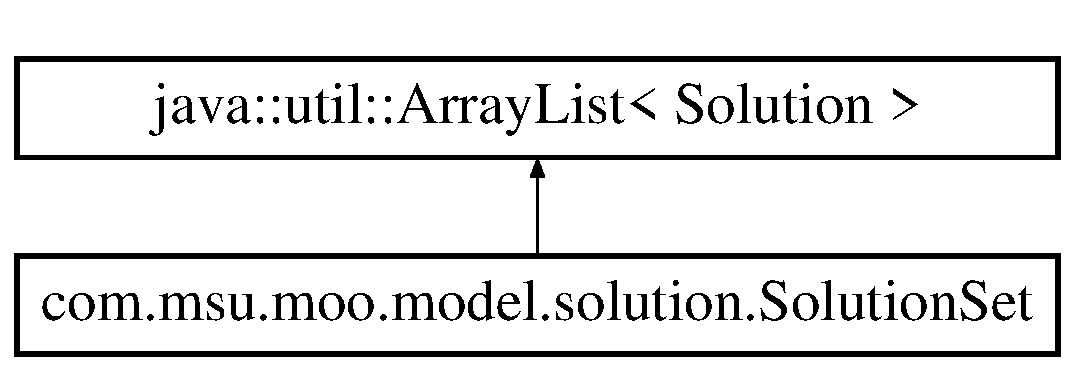
\includegraphics[height=2.000000cm]{classcom_1_1msu_1_1moo_1_1model_1_1solution_1_1SolutionSet}
\end{center}
\end{figure}
\subsection*{Public Member Functions}
\begin{DoxyCompactItemize}
\item 
\hypertarget{classcom_1_1msu_1_1moo_1_1model_1_1solution_1_1SolutionSet_a4ce11410aae86f2432abd8b1b816cde1}{{\bfseries Solution\-Set} (Collection$<$?extends \hyperlink{classcom_1_1msu_1_1moo_1_1model_1_1solution_1_1Solution}{Solution} $>$ c)}\label{classcom_1_1msu_1_1moo_1_1model_1_1solution_1_1SolutionSet_a4ce11410aae86f2432abd8b1b816cde1}

\item 
\hypertarget{classcom_1_1msu_1_1moo_1_1model_1_1solution_1_1SolutionSet_a23207a194f653eb63642111ac7594a94}{{\bfseries Solution\-Set} (int initial\-Capacity)}\label{classcom_1_1msu_1_1moo_1_1model_1_1solution_1_1SolutionSet_a23207a194f653eb63642111ac7594a94}

\item 
void \hyperlink{classcom_1_1msu_1_1moo_1_1model_1_1solution_1_1SolutionSet_aa391e68ec00d6c8baa88c0c51552d2db}{sort\-By\-Objective} (int obj)
\item 
List$<$ Double $>$ \hyperlink{classcom_1_1msu_1_1moo_1_1model_1_1solution_1_1SolutionSet_af8743102447e663dec9267f91b7b0409}{get\-Vector} (int objective)
\item 
\hyperlink{classcom_1_1msu_1_1moo_1_1model_1_1solution_1_1SolutionSet}{Solution\-Set} \hyperlink{classcom_1_1msu_1_1moo_1_1model_1_1solution_1_1SolutionSet_aebb7c5bcbf150314a27655b2947aa7c2}{normalize} ()
\item 
\hyperlink{classcom_1_1msu_1_1moo_1_1model_1_1solution_1_1SolutionSet}{Solution\-Set} \hyperlink{classcom_1_1msu_1_1moo_1_1model_1_1solution_1_1SolutionSet_ae807e94a6e92b9e61de2794d50172d08}{normalize} (List$<$ Pair$<$ Double, Double $>$$>$ boundaries)
\item 
\hyperlink{classcom_1_1msu_1_1moo_1_1model_1_1solution_1_1SolutionSet}{Solution\-Set} \hyperlink{classcom_1_1msu_1_1moo_1_1model_1_1solution_1_1SolutionSet_ae064bd3943d86dba31db36757e485f7f}{invert} (Double max)
\item 
\hypertarget{classcom_1_1msu_1_1moo_1_1model_1_1solution_1_1SolutionSet_a03afab7416e60cfe78c0e7bd04614e33}{Range$<$ Double $>$ {\bfseries get\-Range} ()}\label{classcom_1_1msu_1_1moo_1_1model_1_1solution_1_1SolutionSet_a03afab7416e60cfe78c0e7bd04614e33}

\end{DoxyCompactItemize}


\subsection{Member Function Documentation}
\hypertarget{classcom_1_1msu_1_1moo_1_1model_1_1solution_1_1SolutionSet_af8743102447e663dec9267f91b7b0409}{\index{com\-::msu\-::moo\-::model\-::solution\-::\-Solution\-Set@{com\-::msu\-::moo\-::model\-::solution\-::\-Solution\-Set}!get\-Vector@{get\-Vector}}
\index{get\-Vector@{get\-Vector}!com::msu::moo::model::solution::SolutionSet@{com\-::msu\-::moo\-::model\-::solution\-::\-Solution\-Set}}
\subsubsection[{get\-Vector}]{\setlength{\rightskip}{0pt plus 5cm}List$<$Double$>$ com.\-msu.\-moo.\-model.\-solution.\-Solution\-Set.\-get\-Vector (
\begin{DoxyParamCaption}
\item[{int}]{objective}
\end{DoxyParamCaption}
)\hspace{0.3cm}{\ttfamily [inline]}}}\label{classcom_1_1msu_1_1moo_1_1model_1_1solution_1_1SolutionSet_af8743102447e663dec9267f91b7b0409}
\begin{DoxyReturn}{Returns}
vector of all current solution of given objective 
\end{DoxyReturn}
\hypertarget{classcom_1_1msu_1_1moo_1_1model_1_1solution_1_1SolutionSet_ae064bd3943d86dba31db36757e485f7f}{\index{com\-::msu\-::moo\-::model\-::solution\-::\-Solution\-Set@{com\-::msu\-::moo\-::model\-::solution\-::\-Solution\-Set}!invert@{invert}}
\index{invert@{invert}!com::msu::moo::model::solution::SolutionSet@{com\-::msu\-::moo\-::model\-::solution\-::\-Solution\-Set}}
\subsubsection[{invert}]{\setlength{\rightskip}{0pt plus 5cm}{\bf Solution\-Set} com.\-msu.\-moo.\-model.\-solution.\-Solution\-Set.\-invert (
\begin{DoxyParamCaption}
\item[{Double}]{max}
\end{DoxyParamCaption}
)\hspace{0.3cm}{\ttfamily [inline]}}}\label{classcom_1_1msu_1_1moo_1_1model_1_1solution_1_1SolutionSet_ae064bd3943d86dba31db36757e485f7f}
This method inverts the front. Which means calculate max -\/ current value. If the value is larger than max, it is set to max! 
\begin{DoxyParams}{Parameters}
{\em max} & value for the inversion \\
\hline
\end{DoxyParams}
\begin{DoxyReturn}{Returns}
\hyperlink{classcom_1_1msu_1_1moo_1_1model_1_1solution_1_1Solution}{Solution} that inverted with respect to maximal value 
\end{DoxyReturn}
\hypertarget{classcom_1_1msu_1_1moo_1_1model_1_1solution_1_1SolutionSet_aebb7c5bcbf150314a27655b2947aa7c2}{\index{com\-::msu\-::moo\-::model\-::solution\-::\-Solution\-Set@{com\-::msu\-::moo\-::model\-::solution\-::\-Solution\-Set}!normalize@{normalize}}
\index{normalize@{normalize}!com::msu::moo::model::solution::SolutionSet@{com\-::msu\-::moo\-::model\-::solution\-::\-Solution\-Set}}
\subsubsection[{normalize}]{\setlength{\rightskip}{0pt plus 5cm}{\bf Solution\-Set} com.\-msu.\-moo.\-model.\-solution.\-Solution\-Set.\-normalize (
\begin{DoxyParamCaption}
{}
\end{DoxyParamCaption}
)\hspace{0.3cm}{\ttfamily [inline]}}}\label{classcom_1_1msu_1_1moo_1_1model_1_1solution_1_1SolutionSet_aebb7c5bcbf150314a27655b2947aa7c2}
Normalize by using the boundaries of this set. \hypertarget{classcom_1_1msu_1_1moo_1_1model_1_1solution_1_1SolutionSet_ae807e94a6e92b9e61de2794d50172d08}{\index{com\-::msu\-::moo\-::model\-::solution\-::\-Solution\-Set@{com\-::msu\-::moo\-::model\-::solution\-::\-Solution\-Set}!normalize@{normalize}}
\index{normalize@{normalize}!com::msu::moo::model::solution::SolutionSet@{com\-::msu\-::moo\-::model\-::solution\-::\-Solution\-Set}}
\subsubsection[{normalize}]{\setlength{\rightskip}{0pt plus 5cm}{\bf Solution\-Set} com.\-msu.\-moo.\-model.\-solution.\-Solution\-Set.\-normalize (
\begin{DoxyParamCaption}
\item[{List$<$ Pair$<$ Double, Double $>$$>$}]{boundaries}
\end{DoxyParamCaption}
)\hspace{0.3cm}{\ttfamily [inline]}}}\label{classcom_1_1msu_1_1moo_1_1model_1_1solution_1_1SolutionSet_ae807e94a6e92b9e61de2794d50172d08}
The given boundaries are used for maximum and minimum calculation. \begin{DoxyReturn}{Returns}
normalized front with objectives values between \mbox{[}0,1\mbox{]} 
\end{DoxyReturn}
\hypertarget{classcom_1_1msu_1_1moo_1_1model_1_1solution_1_1SolutionSet_aa391e68ec00d6c8baa88c0c51552d2db}{\index{com\-::msu\-::moo\-::model\-::solution\-::\-Solution\-Set@{com\-::msu\-::moo\-::model\-::solution\-::\-Solution\-Set}!sort\-By\-Objective@{sort\-By\-Objective}}
\index{sort\-By\-Objective@{sort\-By\-Objective}!com::msu::moo::model::solution::SolutionSet@{com\-::msu\-::moo\-::model\-::solution\-::\-Solution\-Set}}
\subsubsection[{sort\-By\-Objective}]{\setlength{\rightskip}{0pt plus 5cm}void com.\-msu.\-moo.\-model.\-solution.\-Solution\-Set.\-sort\-By\-Objective (
\begin{DoxyParamCaption}
\item[{int}]{obj}
\end{DoxyParamCaption}
)\hspace{0.3cm}{\ttfamily [inline]}}}\label{classcom_1_1msu_1_1moo_1_1model_1_1solution_1_1SolutionSet_aa391e68ec00d6c8baa88c0c51552d2db}
Sorts the population by using a specific objective. D\-E\-F\-A\-U\-L\-T\-: Increasing! 
\begin{DoxyParams}{Parameters}
{\em obj} & number of objective \\
\hline
\end{DoxyParams}


The documentation for this class was generated from the following file\-:\begin{DoxyCompactItemize}
\item 
src/main/java/com/msu/moo/model/solution/Solution\-Set.\-java\end{DoxyCompactItemize}

\hypertarget{classcom_1_1msu_1_1moo_1_1operators_1_1mutation_1_1SwapMutation_3_01T_01_4}{\section{com.\-msu.\-moo.\-operators.\-mutation.\-Swap\-Mutation$<$ T $>$ Class Reference}
\label{classcom_1_1msu_1_1moo_1_1operators_1_1mutation_1_1SwapMutation_3_01T_01_4}\index{com.\-msu.\-moo.\-operators.\-mutation.\-Swap\-Mutation$<$ T $>$@{com.\-msu.\-moo.\-operators.\-mutation.\-Swap\-Mutation$<$ T $>$}}
}
Inheritance diagram for com.\-msu.\-moo.\-operators.\-mutation.\-Swap\-Mutation$<$ T $>$\-:\begin{figure}[H]
\begin{center}
\leavevmode
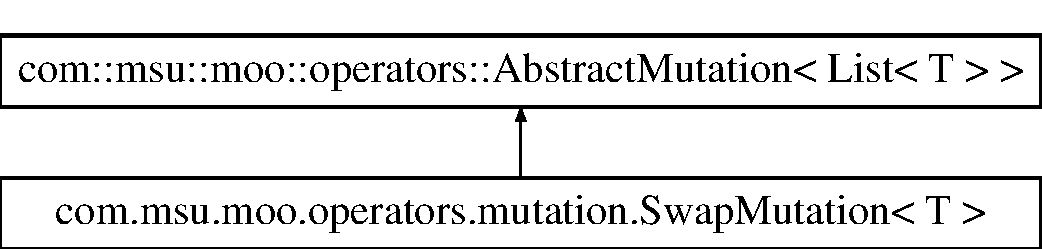
\includegraphics[height=2.000000cm]{classcom_1_1msu_1_1moo_1_1operators_1_1mutation_1_1SwapMutation_3_01T_01_4}
\end{center}
\end{figure}
\subsection*{Protected Member Functions}
\begin{DoxyCompactItemize}
\item 
\hypertarget{classcom_1_1msu_1_1moo_1_1operators_1_1mutation_1_1SwapMutation_3_01T_01_4_ae4b1883a5983fc5c929332762c060316}{void {\bfseries mutate\-\_\-} (List$<$ T $>$ obj)}\label{classcom_1_1msu_1_1moo_1_1operators_1_1mutation_1_1SwapMutation_3_01T_01_4_ae4b1883a5983fc5c929332762c060316}

\end{DoxyCompactItemize}


\subsection{Detailed Description}
This is a Swap\-Mutation which allows to define the range of the mutation. It is only allowed on lists otherwise there will be an error thrown. \begin{DoxyVerb}[0,1,2,3,4] -> swap index 1 and 3 -> [0,3,2,1,4]
\end{DoxyVerb}


The limitation of the swap mutation range could be useful the fix some values. For example an array should only be changed in the middle and not in the beginning.


\begin{DoxyParams}{Parameters}
{\em $<$\-T$>$} & Type which the List is going to have \\
\hline
\end{DoxyParams}


The documentation for this class was generated from the following file\-:\begin{DoxyCompactItemize}
\item 
src/main/java/com/msu/moo/operators/mutation/Swap\-Mutation.\-java\end{DoxyCompactItemize}

\hypertarget{classcom_1_1msu_1_1moo_1_1operators_1_1crossover_1_1UniformCrossover_3_01T_01_4}{\section{com.\-msu.\-moo.\-operators.\-crossover.\-Uniform\-Crossover$<$ T $>$ Class Reference}
\label{classcom_1_1msu_1_1moo_1_1operators_1_1crossover_1_1UniformCrossover_3_01T_01_4}\index{com.\-msu.\-moo.\-operators.\-crossover.\-Uniform\-Crossover$<$ T $>$@{com.\-msu.\-moo.\-operators.\-crossover.\-Uniform\-Crossover$<$ T $>$}}
}
Inheritance diagram for com.\-msu.\-moo.\-operators.\-crossover.\-Uniform\-Crossover$<$ T $>$\-:\begin{figure}[H]
\begin{center}
\leavevmode
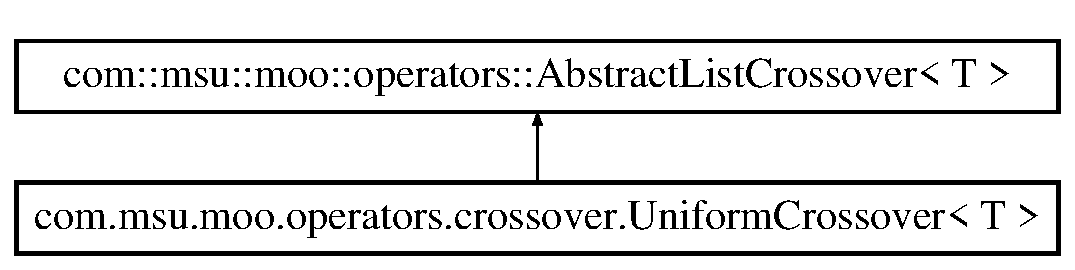
\includegraphics[height=2.000000cm]{classcom_1_1msu_1_1moo_1_1operators_1_1crossover_1_1UniformCrossover_3_01T_01_4}
\end{center}
\end{figure}
\subsection*{Protected Member Functions}
\begin{DoxyCompactItemize}
\item 
\hypertarget{classcom_1_1msu_1_1moo_1_1operators_1_1crossover_1_1UniformCrossover_3_01T_01_4_a221f734a1c5ac26ddef530e88e7d2ddd}{List$<$ List$<$ T $>$ $>$ {\bfseries crossover\-Lists} (List$<$ T $>$ a, List$<$ T $>$ b)}\label{classcom_1_1msu_1_1moo_1_1operators_1_1crossover_1_1UniformCrossover_3_01T_01_4_a221f734a1c5ac26ddef530e88e7d2ddd}

\end{DoxyCompactItemize}


The documentation for this class was generated from the following file\-:\begin{DoxyCompactItemize}
\item 
src/main/java/com/msu/moo/operators/crossover/Uniform\-Crossover.\-java\end{DoxyCompactItemize}

\hypertarget{classcom_1_1msu_1_1moo_1_1util_1_1Util}{\section{com.\-msu.\-moo.\-util.\-Util Class Reference}
\label{classcom_1_1msu_1_1moo_1_1util_1_1Util}\index{com.\-msu.\-moo.\-util.\-Util@{com.\-msu.\-moo.\-util.\-Util}}
}
\subsection*{Static Public Member Functions}
\begin{DoxyCompactItemize}
\item 
static$<$ T $>$ T \hyperlink{classcom_1_1msu_1_1moo_1_1util_1_1Util_ab8093dfa7dd635eb52b81b6cc1941179}{get\-Duplicate} (Hash\-Set$<$ T $>$ hash, Collection$<$ T $>$ c)
\item 
\hypertarget{classcom_1_1msu_1_1moo_1_1util_1_1Util_a7ebea40c5e0234633ad7d6c88fb4ecbb}{static$<$ T $>$ void {\bfseries swap} (List$<$ T $>$ obj, int a, int b)}\label{classcom_1_1msu_1_1moo_1_1util_1_1Util_a7ebea40c5e0234633ad7d6c88fb4ecbb}

\item 
\hypertarget{classcom_1_1msu_1_1moo_1_1util_1_1Util_afdc09b9107801a36a83967f10f5c913e}{static$<$ T $>$ int {\bfseries find} (T\mbox{[}$\,$\mbox{]} array, T value)}\label{classcom_1_1msu_1_1moo_1_1util_1_1Util_afdc09b9107801a36a83967f10f5c913e}

\item 
\hypertarget{classcom_1_1msu_1_1moo_1_1util_1_1Util_a4ff1666542c7f41000ce3e4cda74faa8}{static$<$ T $>$ void {\bfseries write} (String path, T obj)}\label{classcom_1_1msu_1_1moo_1_1util_1_1Util_a4ff1666542c7f41000ce3e4cda74faa8}

\item 
\hypertarget{classcom_1_1msu_1_1moo_1_1util_1_1Util_acb5752270abc3dd834ce096bbee557a6}{static boolean {\bfseries does\-File\-Exist} (String path)}\label{classcom_1_1msu_1_1moo_1_1util_1_1Util_acb5752270abc3dd834ce096bbee557a6}

\end{DoxyCompactItemize}


\subsection{Member Function Documentation}
\hypertarget{classcom_1_1msu_1_1moo_1_1util_1_1Util_ab8093dfa7dd635eb52b81b6cc1941179}{\index{com\-::msu\-::moo\-::util\-::\-Util@{com\-::msu\-::moo\-::util\-::\-Util}!get\-Duplicate@{get\-Duplicate}}
\index{get\-Duplicate@{get\-Duplicate}!com::msu::moo::util::Util@{com\-::msu\-::moo\-::util\-::\-Util}}
\subsubsection[{get\-Duplicate}]{\setlength{\rightskip}{0pt plus 5cm}static $<$T$>$ T com.\-msu.\-moo.\-util.\-Util.\-get\-Duplicate (
\begin{DoxyParamCaption}
\item[{Hash\-Set$<$ T $>$}]{hash, }
\item[{Collection$<$ T $>$}]{c}
\end{DoxyParamCaption}
)\hspace{0.3cm}{\ttfamily [inline]}, {\ttfamily [static]}}}\label{classcom_1_1msu_1_1moo_1_1util_1_1Util_ab8093dfa7dd635eb52b81b6cc1941179}
Return the first duplicate that is found on a given collection


\begin{DoxyParams}{Parameters}
{\em c} & collection of a generic type. \\
\hline
\end{DoxyParams}
\begin{DoxyReturn}{Returns}
first found duplicate 
\end{DoxyReturn}


The documentation for this class was generated from the following file\-:\begin{DoxyCompactItemize}
\item 
src/main/java/com/msu/moo/util/Util.\-java\end{DoxyCompactItemize}

\hypertarget{interfacecom_1_1msu_1_1moo_1_1model_1_1interfaces_1_1VariableFactory_3_01V_01extends_01IVariablebc6c2f25a98dd397b069d7e08412a00f}{\section{com.\-msu.\-moo.\-model.\-interfaces.\-Variable\-Factory$<$ V extends I\-Variable, P extends I\-Problem $>$ Interface Reference}
\label{interfacecom_1_1msu_1_1moo_1_1model_1_1interfaces_1_1VariableFactory_3_01V_01extends_01IVariablebc6c2f25a98dd397b069d7e08412a00f}\index{com.\-msu.\-moo.\-model.\-interfaces.\-Variable\-Factory$<$ V extends I\-Variable, P extends I\-Problem $>$@{com.\-msu.\-moo.\-model.\-interfaces.\-Variable\-Factory$<$ V extends I\-Variable, P extends I\-Problem $>$}}
}
\subsection*{Public Member Functions}
\begin{DoxyCompactItemize}
\item 
V \hyperlink{interfacecom_1_1msu_1_1moo_1_1model_1_1interfaces_1_1VariableFactory_3_01V_01extends_01IVariablebc6c2f25a98dd397b069d7e08412a00f_a656e295c0f79eb4ace5d1f21925a2bce}{create} (P problem)
\end{DoxyCompactItemize}


\subsection{Detailed Description}
This class represents a factory class that should create a \hyperlink{interfacecom_1_1msu_1_1moo_1_1model_1_1interfaces_1_1IVariable}{I\-Variable} or


\begin{DoxyParams}{Parameters}
{\em $<$\-T$>$} & variable type \\
\hline
\end{DoxyParams}


\subsection{Member Function Documentation}
\hypertarget{interfacecom_1_1msu_1_1moo_1_1model_1_1interfaces_1_1VariableFactory_3_01V_01extends_01IVariablebc6c2f25a98dd397b069d7e08412a00f_a656e295c0f79eb4ace5d1f21925a2bce}{\index{com\-::msu\-::moo\-::model\-::interfaces\-::\-Variable\-Factory$<$ V extends I\-Variable, P extends I\-Problem $>$@{com\-::msu\-::moo\-::model\-::interfaces\-::\-Variable\-Factory$<$ V extends I\-Variable, P extends I\-Problem $>$}!create@{create}}
\index{create@{create}!com::msu::moo::model::interfaces::VariableFactory< V extends IVariable, P extends IProblem >@{com\-::msu\-::moo\-::model\-::interfaces\-::\-Variable\-Factory$<$ V extends I\-Variable, P extends I\-Problem $>$}}
\subsubsection[{create}]{\setlength{\rightskip}{0pt plus 5cm}V com.\-msu.\-moo.\-model.\-interfaces.\-Variable\-Factory$<$ V extends {\bf I\-Variable}, P extends {\bf I\-Problem} $>$.create (
\begin{DoxyParamCaption}
\item[{P}]{problem}
\end{DoxyParamCaption}
)}}\label{interfacecom_1_1msu_1_1moo_1_1model_1_1interfaces_1_1VariableFactory_3_01V_01extends_01IVariablebc6c2f25a98dd397b069d7e08412a00f_a656e295c0f79eb4ace5d1f21925a2bce}
Create a new object from the class. The problem information are provided if needed. \begin{DoxyReturn}{Returns}
new random instance. 
\end{DoxyReturn}


The documentation for this interface was generated from the following file\-:\begin{DoxyCompactItemize}
\item 
src/main/java/com/msu/moo/model/interfaces/Variable\-Factory.\-java\end{DoxyCompactItemize}

\hypertarget{classcom_1_1msu_1_1moo_1_1problems_1_1ZDT1}{\section{com.\-msu.\-moo.\-problems.\-Z\-D\-T1 Class Reference}
\label{classcom_1_1msu_1_1moo_1_1problems_1_1ZDT1}\index{com.\-msu.\-moo.\-problems.\-Z\-D\-T1@{com.\-msu.\-moo.\-problems.\-Z\-D\-T1}}
}
Inheritance diagram for com.\-msu.\-moo.\-problems.\-Z\-D\-T1\-:\begin{figure}[H]
\begin{center}
\leavevmode
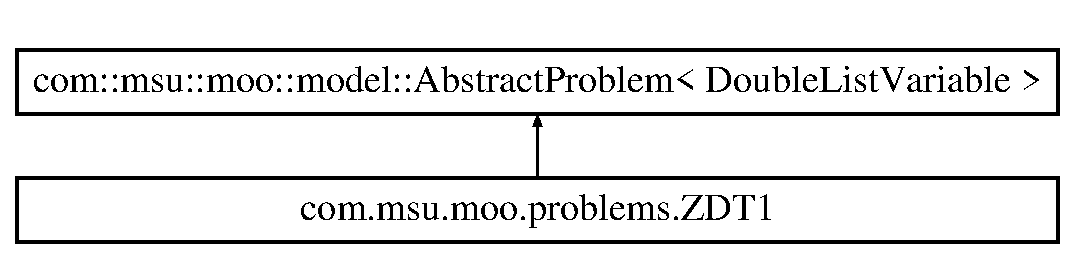
\includegraphics[height=2.000000cm]{classcom_1_1msu_1_1moo_1_1problems_1_1ZDT1}
\end{center}
\end{figure}
\subsection*{Public Member Functions}
\begin{DoxyCompactItemize}
\item 
double \hyperlink{classcom_1_1msu_1_1moo_1_1problems_1_1ZDT1_ab037f1467bf84172ff441cd339a017e3}{eval\-H} (double f, double g)
\item 
\hypertarget{classcom_1_1msu_1_1moo_1_1problems_1_1ZDT1_aee613b615be19f6e765785da95000637}{int {\bfseries get\-Number\-Of\-Objectives} ()}\label{classcom_1_1msu_1_1moo_1_1problems_1_1ZDT1_aee613b615be19f6e765785da95000637}

\end{DoxyCompactItemize}
\subsection*{Protected Member Functions}
\begin{DoxyCompactItemize}
\item 
\hypertarget{classcom_1_1msu_1_1moo_1_1problems_1_1ZDT1_a8f7f43becf40c6080484df819f46a087}{List$<$ Double $>$ {\bfseries evaluate\-\_\-} (\hyperlink{classcom_1_1msu_1_1moo_1_1model_1_1variables_1_1DoubleListVariable}{Double\-List\-Variable} variable)}\label{classcom_1_1msu_1_1moo_1_1problems_1_1ZDT1_a8f7f43becf40c6080484df819f46a087}

\end{DoxyCompactItemize}


\subsection{Detailed Description}
Class representing problem \hyperlink{classcom_1_1msu_1_1moo_1_1problems_1_1ZDT1}{Z\-D\-T1} 

\subsection{Member Function Documentation}
\hypertarget{classcom_1_1msu_1_1moo_1_1problems_1_1ZDT1_ab037f1467bf84172ff441cd339a017e3}{\index{com\-::msu\-::moo\-::problems\-::\-Z\-D\-T1@{com\-::msu\-::moo\-::problems\-::\-Z\-D\-T1}!eval\-H@{eval\-H}}
\index{eval\-H@{eval\-H}!com::msu::moo::problems::ZDT1@{com\-::msu\-::moo\-::problems\-::\-Z\-D\-T1}}
\subsubsection[{eval\-H}]{\setlength{\rightskip}{0pt plus 5cm}double com.\-msu.\-moo.\-problems.\-Z\-D\-T1.\-eval\-H (
\begin{DoxyParamCaption}
\item[{double}]{f, }
\item[{double}]{g}
\end{DoxyParamCaption}
)\hspace{0.3cm}{\ttfamily [inline]}}}\label{classcom_1_1msu_1_1moo_1_1problems_1_1ZDT1_ab037f1467bf84172ff441cd339a017e3}
Returns the value of the \hyperlink{classcom_1_1msu_1_1moo_1_1problems_1_1ZDT1}{Z\-D\-T1} function H.


\begin{DoxyParams}{Parameters}
{\em f} & First argument of the function H. \\
\hline
{\em g} & Second argument of the function H. \\
\hline
\end{DoxyParams}


The documentation for this class was generated from the following file\-:\begin{DoxyCompactItemize}
\item 
src/main/java/com/msu/moo/problems/Z\-D\-T1.\-java\end{DoxyCompactItemize}

\hypertarget{classcom_1_1msu_1_1moo_1_1experiment_1_1impl_1_1ZDT1Experiment}{\section{com.\-msu.\-moo.\-experiment.\-impl.\-Z\-D\-T1\-Experiment Class Reference}
\label{classcom_1_1msu_1_1moo_1_1experiment_1_1impl_1_1ZDT1Experiment}\index{com.\-msu.\-moo.\-experiment.\-impl.\-Z\-D\-T1\-Experiment@{com.\-msu.\-moo.\-experiment.\-impl.\-Z\-D\-T1\-Experiment}}
}
Inheritance diagram for com.\-msu.\-moo.\-experiment.\-impl.\-Z\-D\-T1\-Experiment\-:\begin{figure}[H]
\begin{center}
\leavevmode
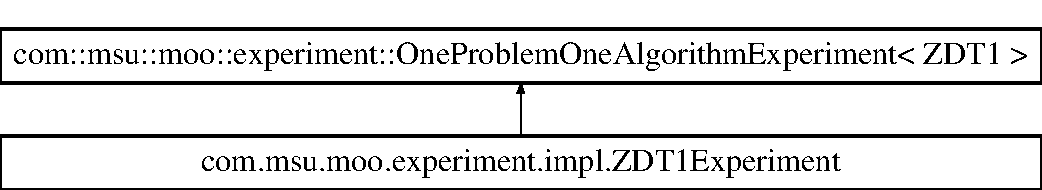
\includegraphics[height=2.000000cm]{classcom_1_1msu_1_1moo_1_1experiment_1_1impl_1_1ZDT1Experiment}
\end{center}
\end{figure}
\subsection*{Static Public Member Functions}
\begin{DoxyCompactItemize}
\item 
\hypertarget{classcom_1_1msu_1_1moo_1_1experiment_1_1impl_1_1ZDT1Experiment_a482e07eac73ecb0612416905379529f8}{static void {\bfseries main} (String\mbox{[}$\,$\mbox{]} args)}\label{classcom_1_1msu_1_1moo_1_1experiment_1_1impl_1_1ZDT1Experiment_a482e07eac73ecb0612416905379529f8}

\end{DoxyCompactItemize}
\subsection*{Protected Member Functions}
\begin{DoxyCompactItemize}
\item 
\hypertarget{classcom_1_1msu_1_1moo_1_1experiment_1_1impl_1_1ZDT1Experiment_afa6fcc19c63e6b2dc11af8fd071a6c59}{I\-Algorithm$<$ \hyperlink{classcom_1_1msu_1_1moo_1_1problems_1_1ZDT1}{Z\-D\-T1} $>$ {\bfseries get\-Algorithm} ()}\label{classcom_1_1msu_1_1moo_1_1experiment_1_1impl_1_1ZDT1Experiment_afa6fcc19c63e6b2dc11af8fd071a6c59}

\item 
\hypertarget{classcom_1_1msu_1_1moo_1_1experiment_1_1impl_1_1ZDT1Experiment_a3c41fa78fcfb88fb3842c66775662f2f}{\hyperlink{classcom_1_1msu_1_1moo_1_1problems_1_1ZDT1}{Z\-D\-T1} {\bfseries get\-Problem} ()}\label{classcom_1_1msu_1_1moo_1_1experiment_1_1impl_1_1ZDT1Experiment_a3c41fa78fcfb88fb3842c66775662f2f}

\item 
\hypertarget{classcom_1_1msu_1_1moo_1_1experiment_1_1impl_1_1ZDT1Experiment_ac9c90e3223196c82152a65c344068730}{\hyperlink{classcom_1_1msu_1_1moo_1_1model_1_1solution_1_1NonDominatedSolutionSet}{Non\-Dominated\-Solution\-Set} {\bfseries get\-True\-Front} ()}\label{classcom_1_1msu_1_1moo_1_1experiment_1_1impl_1_1ZDT1Experiment_ac9c90e3223196c82152a65c344068730}

\end{DoxyCompactItemize}


The documentation for this class was generated from the following file\-:\begin{DoxyCompactItemize}
\item 
src/main/java/com/msu/moo/experiment/impl/Z\-D\-T1\-Experiment.\-java\end{DoxyCompactItemize}

%--- End generated contents ---

% Index
\newpage
\phantomsection
\addcontentsline{toc}{chapter}{Index}
\printindex

\end{document}
